\documentclass[a4paper,11pt,oneside]{article}


















\usepackage{luatexja-fontspec}
\setmainjfont[Path=C:/Windows/Fonts/,BoldFont=yumindb.ttf]{yumin.ttf}
\setsansjfont[Path=C:/Windows/Fonts/,BoldFont=YuGothB.ttc]{YuGothM.ttc}
\renewcommand{\contentsname}{目次}
\renewcommand{\refname}{参考文献}
\renewcommand{\figurename}{図}
\renewcommand{\tablename}{表}
\setlength{\emergencystretch}{2em}

\usepackage[margin=1in]{geometry}
\usepackage{physics}
\usepackage{enumerate}
\usepackage{empheq}
\usepackage{booktabs}
\usepackage{amsmath,amssymb,amsbsy,amstext, amsthm, simplewick}
\usepackage[unicode]{hyperref}
\usepackage{graphicx}
\usepackage{amsfonts}
\usepackage{color}
\usepackage{wasysym}
\usepackage{tikz}

\usepackage{upgreek}
\usepackage{floatrow}
\usepackage{subfig}
\usepackage{xcolor}
\usepackage{dsfont}
\usepackage{tikz}
\usetikzlibrary{decorations.markings}



\usepackage{colortbl}
\definecolor{summersky}{cmyk}{0.71,0.33,0,0.5}
\definecolor{flamingo}{cmyk}{0,0.51,0.71,0.5}
\definecolor{rp}{cmyk}{0.2, 1, 0.6, 0}
\definecolor{pacificblue}{cmyk}{0.95,0.3,0, 0.5}
\definecolor{gray60}{cmyk}{0.4,0.4,0,0.8}

\hypersetup{
    pdftoolbar=true,        
    pdfmenubar=true,        
    pdffitwindow=true,     
    pdfstartview={FitH},    
    pdfnewwindow=true,      
    colorlinks=true,       
    linkcolor=pacificblue,          
    citecolor=flamingo,        
    filecolor=magenta,      
    urlcolor=pacificblue           
}


\theoremstyle{definition}
\newtheorem{definition}{定義}
\setlength{\parindent}{0pt}
\numberwithin{equation}{section}



\newcommand{\enr}[1]{{\color{cyan}(EP: #1)}}
\newcommand{\red}[1]{\color{red}  #1 }
\newcommand{\blue}[1]{\color{blue}  #1 }
\newcommand{\ex}[1]{\langle #1 \rangle}
\newcommand{\expi}[1]{\langle \! \langle #1 \rangle \! \rangle}
\newcommand{\be}{\begin{eqnarray} }
\newcommand{\ee}{\end{eqnarray} }
\newcommand{\bs}{\begin{split} }
\newcommand{\es}{\end{split} }
\newcommand{\non}{\nonumber \\}
\newcommand{\dn}[1]{\delta_{(#1)} }
\newcommand{\tn}[1]{\theta_{(#1)} }
\newcommand{\vk}{\mathbf{k} }
\newcommand{\vq}{\mathbf{q} }
\newcommand{\vv}{\mathbf{v} }
\newcommand{\vx}{\mathbf{x} }
\renewcommand{\v}[1]{\mathbf{#1} }
\newcommand{\intx}{\int_{\mathbf{x}}}
\newcommand{\intq}{\int_{\mathbf{q}}}
\newcommand{\piv}{{\bm \pi} }
\newcommand{\intqn}[1]{\int_{\qv_{#1} } }
\newcommand{\intqp}{\int_{\bf q'}}
\newcommand{\R}{\mathcal{R}}
\renewcommand{\L}{\mathcal{L}}
\renewcommand{\H}{\mathcal{H}}
\newcommand{\cH}{ \mathcal{H} }
\newcommand{\Ll}{\Lambda_{L} }
\newcommand{\Lh}{\Lambda_{H} }
\newcommand{\et}{\tilde \epsilon}
\newcommand{\Mpl}{M_{\mathrm Pl}}
\newcommand{\e}{\epsilon}
\newcommand{\cs}{c_{s}^{2}}
\newcommand{\then}{\quad \Rightarrow\quad}
\renewcommand{\O}{\mathcal{O}}
\newcommand{\bfk}{\mathbf{k}}
\newcommand{\bfp}{\mathbf{p}}
\newcommand{\bfq}{\mathbf{q}}
\newcommand{\bfx}{\mathbf{x}}
\newcommand{\bfy}{\mathbf{y}}



\newcommand{\fpi}{f_{\pi}}
\newcommand{\pir}{\pi_{r}}
\newcommand{\pia}{\pi_{a}}
\newcommand{\dpir}{\dot{\pi}_{r}}
\newcommand{\dpia}{\dot{\pi}_{a}}







\hypersetup{pdftitle={開放系と宇宙論の講義（日本語訳）},pdfauthor={Enrico Pajer},pdfsubject={Lectures on Open Systems and Cosmology / Japanese translation}}
\begin{document}



\begin{titlepage}
\thispagestyle{empty}




\vspace*{2.0cm}



\begin{flushright}
{\scshape Cambridge, 2026}
\end{flushright}



\vspace{3.0cm}











{\sffamily\LARGE\bfseries 開放系と宇宙論の講義\par}



\vspace{3mm}



{\large マスター方程式、Schwinger--Keldysh形式、開放系の有効場理論\par}



\vspace{8mm}



\noindent\rule{\textwidth}{0.8pt}



\vspace{8mm}



\noindent
{\sffamily\large Enrico Pajer}



\vspace{3mm}



\noindent
{\itshape
ケンブリッジ大学 応用数学・理論物理学科\\
Wilberforce Road, Cambridge, CB3 0WA, UK
}



\vspace{5mm}



\noindent
{\itshape E-mail:} \href{mailto:enrico.pajer@gmail.com}{enrico.pajer@gmail.com}



\vspace{1cm}



\noindent
{\scshape 要旨：}
開放系は物理学の至るところに現れる。現実の多くの系は、少なくとも弱く、環境の自由度と相互作用している。これらの自由度は、あまりにも多数であったり、複雑であったり、アクセスできなかったり、未知であったりする。自由度の一部しか観測しない場合、その縮約された動力学は閉鎖系の動力学と質的に異なり、散逸、ノイズ、デコヒーレンス、記憶効果、あるいは観測しないセクターへの情報の流出を示しうる。微視的な記述も未知である場合には、関心のある自由度を系統的に扱う一方、環境と微視的構造は陽に解く代わりにパラメータ化する、開放系の有効記述へと導かれる。



この見方は重力と宇宙論においてとりわけ重要である。インフレーション、暗黒物質、暗黒エネルギーを含む宇宙論の主要な未解決問題には、時空を満たすセクターが関わっており、その微視的な正体は未知で、観測される効果は主として重力的である。同時に、重力系は時間依存性をもつため、保存エネルギーの優先的な定義が存在しないことも多く、非平衡の動力学が自然に現れる。本講義ノートでは、開放系を研究するための道具として演算子形式とSchwinger--Keldysh経路積分を導入し、特に開放系の有効場理論とインフレーションに重点を置く。対象読者は、これらの話題に初めて取り組む修士課程の学生、博士課程の学生、および研究者である。


\vfill


\end{titlepage}


\tableofcontents


 
 
 

\section*{序論}



開放系の理論は、あらゆる物理学者が標準的に身につける道具の一部であるべきだ。現実の系で完全に孤立したものはない。どの系も、少なくとも弱く、自由度があまりにも多数であったり、複雑であったり、アクセスできなかったり、単に未知であったりする環境と相互作用する。これはきわめて一般的な状況であり、開放系の手法は、量子力学と量子情報から、物性物理学、統計物理学、素粒子物理学、宇宙論、一般相対論まで、事実上あらゆる物理学の分野に応用される。本ノートの目的は、ある部分系が相互作用するすべての対象の完全な微視的状態を追跡せずに、その部分系の動力学を記述するための基本的な道具をいくつか導入することである。



\paragraph{重力と宇宙論への開放系からのアプローチ。} 開放系は\textit{宇宙論}において特に自然に現れる。宇宙論の主要な未解決問題は、おおむねインフレーション、暗黒物質、暗黒エネルギーの問題に要約できる。数十年にわたり精力的に研究されてきたこれらの問題には、際立った共通点がある。
第一に、いずれも時空を満たす成分、セクター、あるいは有効媒質に関わる。インフレーションとは、高温ビッグバン以前の宇宙を満たし、初期の加速膨張期を引き起こした物理に与えた名前であり、暗黒エネルギーは現在の加速膨張を担う成分を指す。暗黒物質も、晩期には完全に一様ではなく集積しているものの、時空を満たす成分であり、その存在はほぼ全面的に重力効果を通じて推測される。このため、これらの問題を、孤立して準備・研究できる真空上を粒子が伝播すると考える通常の素粒子物理の問題として捉えるのは自然ではない。むしろ、関心のある動力学、この場合は重力の動力学が媒質の内部で起こる、物性物理の問題に精神的に近い。



第二に、これらすべての場合で微視的な物理が未知である。これは、微視的な法則は分かっていても、そこから生じる動力学を実際に解くのが困難という、QCDや複雑な物質でおなじみの状況にとどまらない。宇宙論では、微視的自由度そのものが全く分からないことが多い。インフレーション、暗黒物質、暗黒エネルギーのモデルは多数あるにもかかわらず、これらが実際に何なのかは分かっていない。このことは、有効場理論の立場をほぼ必然的に要請する。すなわち、微視的物理の詳細については可能な限り特定の仮定を置かず、関係する自由度と、それらを制約する対称性を同定するのである。



第三に、現在の観測から分かる限り、これらのセクターは可視世界と主として、あるいは重力のみを通じて相互作用する。例えば、再加熱が起こるためにはインフラトンが最終的に標準模型と相互作用するはずだと考えられるが、その相互作用を直接観測することはできない。同様に、膨大な実験的努力にもかかわらず、暗黒物質と標準模型粒子の間の非重力的相互作用を示す肯定的な証拠は、まだ得られていない。この意味で、宇宙論は自然に開放系の問題となる。重力の自由度、すなわち計量そのものがアクセス可能な系であり、宇宙を満たす未知の成分が環境として働く。より一般には、系と環境の具体的な分け方は問いに依存しうる。系は計量、曲率摂動、長波長モードの集合、あるいはその他のアクセス可能な自由度の集合でありうる。したがって、得られる記述は\textit{開放系の有効場理論}となる。環境の微視的構造が未知であるという意味で有効理論であり、環境の自由度を無視したとき、観測する重力の自由度がユニタリに発展するとは限らないという意味で開放系なのである。



開放系の考え方は、より広く一般相対論にも深く関わっている。重力はあらゆるものと相互作用するため、真に閉じた系の記述には、原理的には宇宙のすべての自由度を記述する必要があるが、それは実行可能でも有用でもない。さらに、物質を導入すると、重力は通常、時間依存する時空を生じさせることで応答する。そのような背景では時間的Killingベクトルが存在するとは限らず、したがって時間並進に対応する保存エネルギーも存在するとは限らない。これは、エネルギー保存により低エネルギーでは重い自由度が効率よく励起されないために、それらを積分消去できるという、最もなじみ深いWilsonianな直観に対する重大な障害である。時間依存する重力背景では、この議論が成り立たないことがある。重い場が背景の発展によって励起され、その後、軽いセクターに対する環境自由度として働きうるからである。一般相対論には地平線もあり、系の一部へのアクセスに、場合によっては原理的にも、さらなる障害をもたらす。本ノートでは地平線に重点を置かないが、それらは重力物理学において開放量子系の手法を発展させる重要な追加の動機となる。\\



密接に関連する論点は、開放系が一般に\textit{非平衡}であることだ。背景の時間依存性が小さな摂動ではなく、まさに記述したい現象そのものである宇宙論では、これは本質的である。平衡熱力学には膨大な関心が寄せられてきており、多くの状況で適切な言葉を提供する。しかし、本ノートの動機となる宇宙論的状況は、通常、平衡状態ではない。そのため、明示的に断らない限り熱平衡への特殊化を避け、一般的な非平衡過程を記述できる柔軟性を形式論に持たせる。この点は重力物理学でも重要である。時空が時間的Killingベクトルをもつ場合、あるいは適切な解析接続を定義できるだけの対称性をもつ場合には、ブラックホールや適切なde Sitterパッチでのように、しばしばEuclid幾何へWick回転し、熱的な解釈を引き出せる。しかし、現実的な重力や宇宙論の多くの問題には、それほどの対称性はない。それらはLorentz的な非平衡の動力学的問題として扱うべきである。そもそも、宇宙史を通じた構造形成が明らかに示すように、私たちの宇宙は平衡からはるかに遠い。



\paragraph{ねらいと目標。} 本講義ノートの主な目的は、しばしば別々に論じられる三つの主題、すなわち演算子形式における開放量子系、Schwinger--Keldysh経路積分、宇宙論を結びつけることである。演算子形式と量子マスター方程式は、特に量子情報や量子光学において、開放量子系に関する多くの議論の自然な言葉となる。経路積分形式は原理的には等価だが、異なる研究共同体で用いられることが多く、場の量子論、ゲージ理論、重力には欠かせない。宇宙論は、量子場、時間依存する背景、重力の拘束条件、原始揺らぎに関する観測的な問いを組み合わせるため、さらに一層の構造を加える。この三つの主題は互いに多くを教え合える。ある領域の結果や直観を別の領域へ持ち込むことで進展が得られるが、必要な内容が統一した記法と共通の教育的水準で提示されることはまれであり、それは容易ではない。\\



本ノートが採る\textit{分野横断的な視点}は、今日とりわけ価値がある。人工知能の急速な発展は、研究者の学び方と働き方を変えつつある。物理学者が分野の境界を越え、不慣れな道具を習得し、もともとの専門領域の外で着想を試すことが、ますます現実的になっている。最近利用可能になったAIの道具により、研究者は、不慣れな文献を読み進め、計算を確認し、隣接分野の言葉を習得するうえで、ますます強力な支援を得ている。このことは、学際的研究を恐れず、野心的な問いにより大胆に取り組むよう、私たちを後押しするはずだ。互いにほとんど交流しない、ますます専門化した道筋を進む代わりに、ある問題に本当に必要な道具を見定め、それらを効率よく学ぶことができる。本ノートはその精神で書かれた。網羅性を目指すのではなく、研究共同体の橋渡しをし、学生や研究者が演算子法、経路積分、宇宙論的応用の間を行き来しやすくすることを目指す。\\



本ノートは、開放量子系、Schwinger--Keldysh形式、あるいは非平衡宇宙論に初めて取り組む修士課程の学生、博士課程初期の学生、および研究者を対象とする。そのため、密度行列の基本理論や標準宇宙論の初歩など、多くの読者がすでに他で学んだかもしれない入門的な内容も含めた。その目的は、ノートを自己完結的にするだけでなく、より高度な話題に進む前に記法と規約を定めることにもある。重点は、文献を読み始めるために必要な主要な定義、方程式、例、概念的構造をそろえ、実用的な道具立てを築くことに置く。より専門的で研究段階の発展については、大部分を参考文献に委ねる。



本ノートは2026年に三つのスクールで行った講義のために準備された。イタリアのPadovaにあるScuola Galileiana di Studi Superioriで「基本相互作用の理論物理学」を主題として開催された\href{https://scuolagalileiana.unipd.it/wp-content/uploads/2026/03/Scuola-tematica-fisica-DEF.pdf}{Scuola Tematica}、「宇宙論的相関関数」を主題とする\href{https://indico.math.cnrs.fr/event/15597/}{2026年IHESサマースクール}、そしてスペインのCastro Caldelas、As Barreirasで「無秩序な宇宙」を主題として開催された\href{https://indico.global/event/16455/overview}{La Ricotta Summer School}である。したがって、教育的な利用を意図している。関心ある読者が、開放量子系、Schwinger--Keldysh有効作用、宇宙論的応用に関する現代の文献に取り組み、やがて自らの研究でこれらの道具を使うための、確かな基礎となることを願っている。





\paragraph{本ノートの構成。} 第\ref{sec:1}節では、密度行列、複合系、部分トレース、エンタングルメント、デコヒーレンスを含む、開放系の量子力学を概観する。第\ref{sec:2}節では、縮約動力学、量子チャネル、力学写像、GKSLマスター方程式を導入し、その微視的な起源と、時間依存する写像およびCP可分性への拡張も扱う。第\ref{sec:3}節では、量子ビットと散逸調和振動子を例として、Lindblad方程式の具体的な解を論じる。



第\ref{sec:4}節では、二重化した時間経路とKeldysh基底から、Feynman--Vernon影響汎関数とその一般的な整合性条件まで、Schwinger--Keldysh形式を展開する。第\ref{sec:SKmap}節では、局所的なSchwinger--Keldysh作用を力学写像および完全正値性と関連づけ、ジャンプ演算子、Langevin動力学、散逸するスカラー場を論じる。第\ref{sec:5}節では、宇宙論的背景、インフレーションの相関関数、原始非ガウス性を概観する。第\ref{sec:6}節では、インフレーションの開放有効場理論を構築し、パワースペクトルとバイスペクトルに適用する。第\ref{sec:stochastic}節では、確率的インフレーションを導入し、Langevin記述とFokker--Planck記述を用いて、de Sitter時空における永年成長と晩期の振る舞いを研究する。付録Aでは、二次のSchwinger--Keldysh核の逆を求める際に有用な結果をまとめる。





\subsection*{参考文献と資料}



ここでは、本ノートの作成に用いた参考文献をまとめ、文献に見られる数多くの資料の中から、有用なものを選んで紹介する。



密度行列の入門的な説明は、ほぼどの量子力学の教科書にも見つかる。第\ref{sec:1}節は、ケンブリッジ大学数学Triposの「量子力学の原理」の講義と、David Skinnerによる優れた講義ノート\cite{Skinner}に沿っている。



開放量子系の古典的かつ包括的な教科書として、BreuerとPetruccioneの著書\cite{breuerTheoryOpenQuantum2002}がある。第\ref{sec:2}節と第\ref{sec:3}節の記述は、一部この文献に沿っている。同書では演算子形式と確率的手法により重点が置かれているが、きわめて幅広い話題と応用が収められている。



開放系のSchwinger--Keldysh経路積分についての優れた参考書は、Alex Kamenevの著書\cite{kamenev_2011}である。この教科書は基礎から積み上げ、量子多体系への多数の応用を提示している。量子多体物理学の言葉で書かれているため、高エネルギー物理学を背景とする読者には、慣れるまで少し時間がかかるかもしれない。第\ref{sec:4}節の一部はこの文献に基づいている。



宇宙論とインフレーションの概説は、ケンブリッジ大学数学Tripos Part IIIの「宇宙論」\cite{PajerCosmologyNotes}および「宇宙論における場の理論」\cite{PajerFieldTheoryCosmologyNotes}の講義のために私が書いた講義ノートに基づく。閉鎖系でのSchwinger--Keldysh経路積分の摂動展開については、文献\cite{Chen:2017ryl}が優れた参考資料である。第\ref{sec:6}節は主として原著論文\cite{Creminelli:2006xe,Cheung:2007st,LopezNacir:2011kk,Salcedo:2024smn,Salcedo:2026sdn}に基づく。



de Sitter時空の軽い場と確率的インフレーションについては、非常に優れたレビュー\cite{Woodard:2025cez,Cruces:2022imf,Vennin:2020kng}が多数あり、本講義で提示する初歩的な議論よりもはるかに高度な側面も論じられている。確率的インフレーション、およびすべての量子効果を系統的に捉えるための最低次の記述の改良に関しては、何百もの論文がある。これらの問題はいずれも詳しくは論じず、上記のレビューとそこに挙げられた文献を読者に勧める。\\



開放量子系には、さまざまな観点から問題の異なる側面を論じた優れたレビューが多数ある。影響汎関数、ノイズ、デコヒーレンス、宇宙論を結びつける補完的な場の理論による取り扱いは、CalzettaとHu\cite{Calzetta:2008iqa}に与えられている。現代的なSchwinger--Keldysh有効理論と非Markov的量子動力学は、それぞれ文献\cite{Liu:2018kfw,RivasHuelgaPlenio2014}で概説されている。Hong LiuとPaolo Gloriosoの先駆的な研究は、この主題についての私の理解に特に大きな影響を与えた。T.~Colasによるごく最近の優れたレビュー\cite{Colas:2025app}は、インフレーションと晩期宇宙の重力への、開放量子系およびSchwinger--Keldysh経路積分の応用を論じている。そこでは開放系の有効場理論の構築が強調され、この分野の最新の進展の一部も扱われている。もう一つの優れた参考資料は、L.~M.~Sieberer、M.~Buchhold、S.~Diehlによるレビュー\cite{2016RPPh...79i6001S}であり、駆動された開放量子系、特に冷却原子と光共振器への応用に重点が置かれている。








\section{開放系の量子力学}\label{sec:1}



量子力学の標準的な定式化は、孤立したHilbert空間内をユニタリに発展する状態ベクトルで記述される閉鎖系から始まることが多い。しかし、多くの物理的状況では、この記述は実用的でないか、不完全である。微視的状態について確率的な情報しか得られない場合もあれば、より大きな複合系の部分系に関心がある場合もあり、観測する自由度が、アクセス不能な、あるいは詳細にモデル化するには複雑すぎる環境と相互作用している場合もある。こうした状況が、密度行列形式、そしてより一般には開放量子系の枠組みを動機づける。この枠組みでは、基本的な対象は必ずしも純粋状態ではなく、密度行列である。密度行列によって、純粋状態、統計混合、そして後に扱う、観測しない自由度についてトレースを取って得られる縮約状態を記述できる。



本節の目的は、本ノートの以後の部分に必要な、量子力学の基本的な道具を導入することである。まず密度行列とその解釈から始め、次に量子ビットやBlochベクトルなどの簡単な例を論じ、その後、複合系、テンソル積、部分トレース、エンタングルメント、デコヒーレンスに進む。これらの概念は概念的に重要であるだけでなく、開放系の動力学を定式化する自然な言葉にもなる。特に、全体系が純粋状態を保ち、ユニタリに発展していても、部分系が純粋状態から混合状態へ発展しうることを明らかにする。この内容にすでに親しんでいる読者も多いだろう。その場合は、直接次節へ進んでもよい。


  
 

\subsection{密度行列}



多くの物理的状況では、量子系を単一の状態ベクトルで記述することは、不便であるか、不十分である。これは、系が異なる状態に確率的にしか準備されないためである場合もあれば、その正確な微視的状態を知らないためである場合もあり、あるいは後に、より大きな量子系の部分系を記述したくなるためである場合もある。こうした考察が、密度行列とも呼ばれる密度演算子の導入を動機づける。



系の量子状態について、古典的な確率情報しかもっていないとしよう。この追加の不確定性は、量子力学に標準的に備わる確率的性質に重ねて加わるものである。そこで、系が規格化された状態$|\psi_\alpha\rangle \in \mathcal H$に\textit{古典的な}確率$p_\alpha$であると考えよう。ここで
\begin{equation}
0 \le p_\alpha \le 1,
\qquad
\sum_\alpha p_\alpha = 1,
\qquad
\langle \psi_\alpha | \psi_\alpha \rangle = 1 .
\end{equation}
状態$|\psi_\alpha\rangle$は互いに直交している必要はない。ここで、系が状態$ |\psi_\alpha\rangle $の線形重ね合わせにあると言っている\textit{のではない}ことを強調しておく。それならば、単にHilbert空間内の別の一つの状態にすぎないからである。



この場合、観測量をどのように取り出せばよいだろうか。$Q$が物理的観測量に対応するHilbert空間上の線形Hermite演算子であるなら、その期待値は
\begin{equation}
\langle Q \rangle
=
\sum_\alpha p_\alpha \, \langle \psi_\alpha | Q | \psi_\alpha \rangle .
\end{equation}
系の状態についてもっている情報を一つの量にまとめると便利である。次の演算子がその役割を果たすことが分かる。
\begin{equation}
\rho \equiv \sum_\alpha p_\alpha \, |\psi_\alpha\rangle \langle \psi_\alpha | ,
\end{equation}
$ \rho$を密度行列と呼ぶ\footnote{同義の名称として密度演算子がある。残念ながら、どちらの用語にも難点がある。「行列」という語は有限次元Hilbert空間を連想させるが、本ノートでは無限次元Hilbert空間の場合にも「線形演算子」と同じ意味で用いる。一方、「演算子」という語は物理的観測量を連想させるが、ここでは$ \rho$は系の\textit{状態}を表している。}。



この定義の利点は、期待値が次の簡潔な形に書けることにある。
\begin{equation}\label{traceQ}
\langle Q \rangle = \Tr_{\mathcal H}(\rho Q) \,,
\end{equation}
ここで$ \Tr$はトレース操作である。有限次元Hilbert空間ではトレースはよく知られたものだが、無限次元空間では微妙な問題が生じうる。より形式的には、トレースは、演算子の適切な線形空間$\mathcal A$上で定義された写像$\Tr$であり、すべての$A,B\in\mathcal A$とすべての複素数$a,b$に対して線形性
\begin{equation}
\Tr(aA+bB)=a\,\Tr(A)+b\,\Tr(B) ,
\end{equation}
および、両方の積が定義域に属する場合の巡回性
\begin{equation}
\Tr(AB)=\Tr(BA) ,
\end{equation}
を満たす。ここでいう定義域は$\Tr$の定義域である。さらに正値性\footnote{忠実性、すなわち$\Tr(A^\dagger A)=0$ならば$A=0$であることも要求する場合が多い。}
\begin{equation}
\Tr(A^\dagger A)\ge 0 .
\end{equation}
も満たす。無限次元では、トレースは一般にすべての有界演算子に対して定義されるわけではなく、「トレース級」演算子のような適切な部分集合に対してのみ定義される。本ノートではこれらの問題には立ち入らず、トレースが常に適切に定義されていると仮定する。



\eqref{traceQ}が$ Q$の期待値を計算することを確かめるため、$\{|q_n\rangle\}$を$Q$の固有状態からなる正規直交基底とする。したがって
\begin{equation}
Q = \sum_n q_n |q_n\rangle\langle q_n| .
\end{equation}
すると
\begin{align}
\Tr_{\mathcal H}(\rho Q)
&= \sum_n \langle q_n | \rho Q | q_n \rangle \\
&= \sum_{n,\alpha} p_\alpha \, \langle q_n | \psi_\alpha \rangle \langle \psi_\alpha | Q | q_n \rangle \\
&= \sum_{n,\alpha} p_\alpha \, q_n \, |\langle q_n | \psi_\alpha \rangle|^2 \\
&= \sum_\alpha p_\alpha \, \langle \psi_\alpha | Q | \psi_\alpha \rangle = \langle Q \rangle .
\end{align}
となる。このように、密度行列は、任意の観測量の期待値を計算するために必要なすべての情報を含んでいる。



特に重要な特殊例は、系が単一の規格化された状態$|\psi\rangle$で記述される場合である。この場合には
\begin{equation}
\rho = |\psi\rangle\langle\psi| ,
\end{equation}
となり、トレースによる公式は通常の表式
\begin{equation}
\Tr(\rho Q) = \langle \psi | Q | \psi \rangle .
\end{equation}


に帰着する。ここで、密度行列の一般的な性質をまとめよう。密度演算子$\rho : \mathcal H \to \mathcal H$は、次を満たさなければならない\footnote{半正定値性を、略記$ \rho \geq 0$で表すこともある。}。
\begin{align}
\rho^\dagger &= \rho , \\
\langle \phi | \rho | \phi \rangle &\ge 0
\qquad \text{任意の } |\phi\rangle \in \mathcal H , \\
\Tr \rho &= 1 .
\end{align}
これらの条件はそれぞれ、$\rho$がHermiteであること、半正定値であること、トレースが1となるように規格化されていることを意味する。



逆に、これら三つの性質を満たす任意の演算子は、正当な密度行列である。実際、簡単のため有限次元を仮定すると、$\rho$はHermiteであるから、スペクトル分解
\begin{equation}
\rho = \sum_n p_n |n\rangle\langle n| ,
\end{equation}
をもつ。ここで固有値$p_n$は実数である。正値性から
\begin{equation}
p_n \ge 0 ,
\end{equation}
が従い、一方、トレース条件から
\begin{equation}
\sum_n p_n = 1 .
\end{equation}
が得られる。したがって、$\rho$は常に、正規直交状態$|n\rangle$の確率的混合として解釈できる。



$\rho$の行列要素、すなわち
\begin{align}
\rho_{nm}:=\langle n | \rho | m\rangle\,,
\end{align}
が任意の正規直交基底で有界であることにも注意しておくとよい。対角成分は
\begin{equation}
\rho_{nn} \ge 0,
\qquad
\sum_n \rho_{nn} = 1,
\qquad
\Rightarrow
\qquad
\rho_{nn} \le 1 .
\end{equation}
を満たす。さらに、正値性から次の上界が従う。
\begin{align}
|\rho_{nm}|
&:= |\langle n|\rho|m\rangle|
\nonumber\\
&= |\langle n|A^\dagger A|m\rangle|
\qquad
\text{ただし } \rho \ge 0 \;\Rightarrow\; \rho = A^\dagger A
\nonumber\\
&= |\langle An|Am\rangle|
\nonumber\\
&\le \sqrt{\langle An|An\rangle}\,\sqrt{\langle Am|Am\rangle}
\qquad \text{(Cauchy--Schwarz)}
\nonumber\\
&= \sqrt{\langle n|A^\dagger A|n\rangle}\,\sqrt{\langle m|A^\dagger A|m\rangle}
\nonumber\\
&= \sqrt{\langle n|\rho|n\rangle}\,\sqrt{\langle m|\rho|m\rangle}
\nonumber\\
&= \sqrt{\rho_{nn}\rho_{mm}} .
\end{align}
したがって、$ n\neq m$に対して$  |\rho_{nm}| \le \frac12  $である。




\paragraph{純粋状態と混合状態} 次に、純粋状態と混合状態の区別に進む。規格化されたベクトル$|\chi\rangle \in \mathcal H$が存在して
\begin{equation}
\rho = |\chi\rangle\langle\chi| .
\end{equation}
と書ける場合、その状態を\textit{純粋}という。そうでなければ、その状態を\textit{混合}という。



この定義には、いくつかの等価な特徴づけがある。まず、$\rho = |\psi\rangle\langle\psi|$ならば
\begin{equation}
\rho^2
=
|\psi\rangle\langle\psi|\psi\rangle\langle\psi|
=
|\psi\rangle\langle\psi|
=
\rho .
\end{equation}
である。したがって、どの純粋状態も$ \rho^2 = \rho   $を満たす。逆に、
\begin{equation}
\rho^2 = \rho .
\end{equation}
を仮定しよう。$\rho$の固有基底では
\begin{equation}
\rho |n\rangle = p_n |n\rangle ,
\end{equation}
となるので、条件$\rho^2=\rho$は
\begin{equation}
p_n^2 = p_n .
\end{equation}
を意味する。したがって各固有値は$0$または$1$である。$\Tr \rho = 1$であるから、ちょうど一つの固有値が$1$に等しく、残りはすべてゼロである。よって、ある規格化された状態に対して
\begin{equation}
\rho = |\chi\rangle\langle\chi|
\end{equation}
と書ける。この規格化された状態が$|\chi\rangle$であり、状態は純粋である。以上から、次が示された。
\begin{equation}
\rho \text{ は純粋}
\qquad \Longleftrightarrow \qquad
\rho^2 = \rho .
\end{equation}
このことから、次の自明な系が得られる。整数$ n\geq 2$について
\begin{equation}
\rho \text{ は純粋}
\qquad \Longleftrightarrow \qquad
\rho^n = \rho \,.
\end{equation}
である。さらに別の等価な条件は
\begin{equation}
\Tr \rho^2 = 1 .
\end{equation}
である。実際、$\rho$が純粋ならば$\rho^2=\rho$であるから、
\begin{equation}
\Tr \rho^2 = \Tr \rho = 1 .
\end{equation}
となる。逆に、対角基底では
\begin{equation}
\Tr \rho^2 = \sum_n p_n^2 .
\end{equation}
である。$p_n \ge 0$および$\sum_n p_n = 1$であるから、
\begin{equation}
\sum_n p_n^2 \le 1 ,
\end{equation}
となり、等号が成立するのは、一つの固有値が$1$に等しく、その他がすべてゼロの場合、かつその場合に限る。したがって
\begin{equation}
\Tr \rho^2 = 1
\qquad \Longleftrightarrow \qquad
\rho \text{ は純粋}.
\end{equation}


である。より一般には、混合状態に対して
\begin{equation}
0 < \Tr \rho^2 < 1 .
\end{equation}


が成り立つ。純粋性の等価な判定条件をまとめると、
\begin{align}
\rho \text{ は純粋}
&\Longleftrightarrow
\rho = |\chi\rangle\langle\chi| \text{ ある規格化された } |\chi\rangle \nonumber\\
&\Longleftrightarrow
\rho^2 = \rho \nonumber\\
&\Longleftrightarrow
\Tr \rho^2 = 1 .
\end{align}
となる。これらの条件が満たされない場合、状態は混合状態である。密度行列は、開放量子系を論じる際の自然な出発点となる。





\paragraph{von Neumannエントロピー} 密度行列$\rho$が与えられたとき、そのvon Neumannエントロピーを次で定義する。
\begin{equation}
S(\rho) := - \Tr(\rho \ln \rho) \,.
\end{equation}
一見すると恣意的に見えるこの操作は、古典的な\textit{情報理論}に根ざしており、Shannonエントロピーと密接に関連する。ある密度行列のvon Neumannエントロピーは、対応する量子状態の本質的な性質を捉える。これは決して唯一のエントロピーの概念ではないが、実際、次の小節でもさらにいくつかに出会うことになるが、量子情報理論と開放系の研究で、とりわけ重要な役割を果たす。



$ \rho$はHermite演算子なので、対角化できる。$\rho$のスペクトル分解が
\begin{equation}
\rho = \sum_n p_n |n\rangle\langle n| \,,
\qquad
p_n \ge 0 \,,
\qquad
\sum_n p_n = 1 \,,
\end{equation}
であるなら、$\rho$の台の上で$\ln \rho = \sum_n (\ln p_n) |n\rangle\langle n|$であることから、エントロピーは
\begin{equation}\label{Sdiag}
S(\rho) = - \sum_n p_n \ln p_n \,,
\end{equation}
となる。ここでは、$x \to 0^+$のとき$x \ln x \to 0$とする標準的な規約を用いる。したがって、von Neumannエントロピーは$\rho$の固有値のみに依存し、計算に用いる基底には依存しない。表式\eqref{Sdiag}は、von NeumannエントロピーをShannonエントロピーの量子版とみなせることを明示している。



密度行列の固有値は$0 \le p_n \le 1$を満たすため、$\ln p_n \le 0$であり、したがって
\begin{equation}
S(\rho) \ge 0 \,.
\end{equation}
となる。さらに、
\begin{equation}
S(\rho)=0
\qquad \Longleftrightarrow \qquad
\rho \text{ は純粋}.
\end{equation}
が成り立つ。実際、$\rho$が純粋ならば、その固有値は$1,0,0,\dots$であるから、
\begin{equation}
S(\rho) = - 1 \cdot \ln 1 = 0 \,.
\end{equation}
となる。逆に、$S(\rho)=0$ならば
\begin{equation}
0 = - \sum_n p_n \ln p_n \,.
\end{equation}
である。$0\le x \le 1$に対して$-x \ln x \ge 0$なので、和の各項は非負である。よって、各項はすべてゼロでなければならない。しかし、$-p_n \ln p_n =0$となるのは$p_n=0$または$p_n=1$の場合に限られる。固有値の和は$1$なので、ちょうど一つの固有値が$1$に等しく、その他はすべてゼロでなければならない。したがって、$\rho$は純粋である。



Hilbert空間が有限次元であり、
\begin{equation}
d := \dim \mathcal H < \infty \,,
\end{equation}
ならば、エントロピーは上から
\begin{equation}
S(\rho) \le \ln d \,.
\end{equation}
で抑えられる。この上界は、規格化の拘束条件$\Tr \rho =1$のもとでエントロピーの極値を求めることで得られる。Lagrange未定乗数$\lambda$を導入して、次の極値を求める。
\begin{equation}
\Phi[\rho,\lambda] := S(\rho) - \lambda \bigl(1-\Tr \rho \bigr) \,.
\end{equation}
$\rho$について変分すると
\begin{align}
0 = \delta \Phi
&= - \Tr\!\left[\delta \rho \bigl(\ln \rho + 1 - \lambda \bigr)\right] .
\end{align}
を得る。これは任意の$\delta \rho$に対して成り立たなければならないため、
\begin{equation}
\ln \rho + 1 - \lambda = 0 \,,
\end{equation}
が得られ、したがって
\begin{equation}
\rho = e^{\lambda-1}\,\mathds{1} _{\mathcal H} \,.
\end{equation}
となる。$\Tr \rho =1$を課すと
\begin{equation}
1 = \Tr \rho = e^{\lambda-1}\Tr \mathds{1} _{\mathcal H} = e^{\lambda-1} d \,,
\end{equation}
を得るので、
\begin{equation}
\rho_{\max} = \frac{1}{d}\,\mathds{1} _{\mathcal H} \,.
\end{equation}
である。この状態でエントロピーを評価すると、
\begin{equation}
S_{\max}
=
-\Tr\!\left(\frac{1}{d}\mathds{1} _{\mathcal H}\ln \frac{1}{d}\mathds{1} _{\mathcal H}\right)
=
-\Tr\!\left(\frac{1}{d}\mathds{1} _{\mathcal H}\right)\ln \frac{1}{d}
=
\ln d \,.
\end{equation}
を得る。このように、von Neumannエントロピーは最大混合状態
\begin{equation}
\rho = \frac{1}{d}\,\mathds{1} _{\mathcal H} \,,
\end{equation}
で最大となる。この状態では、すべての状態が等しい確率をもつ。この結果は、エントロピーが大きいほど、系の正確な量子状態についての不確定性が大きい、あるいは同じことだが情報が少ない、という直観を与える。





\paragraph{熱的密度行列とGibbs分布} 物理学で際立った役割を果たす密度行列として、熱的密度行列がある。この特定の選択は非常に重要な役割を果たすため、ときには、ある密度行列が非熱的であるとわざわざ断る必要を感じることさえある。実際には、測度ゼロの集合を除くすべての密度行列が非熱的であるにもかかわらず、である。密度行列形式は量子統計力学に不可欠である。ここでは、ごく手短に述べるにとどめる。規格化条件
\begin{equation}
\Tr \rho = 1 \,,
\end{equation}
に加えて、平均エネルギーも
\begin{equation}
\Tr(\rho H)=U \,.
\end{equation}
に固定するとしよう。ここで、両方の拘束条件のもとでエントロピーの極値を求める。Lagrange未定乗数$\lambda$と$\beta$を導入して、次を考える。
\begin{equation}
\Phi[\rho,\lambda,\beta]
:=
S(\rho)-\lambda\bigl(1-\Tr \rho \bigr)-\beta\bigl(\Tr(\rho H)-U\bigr) \,.
\end{equation}
その変分は
\begin{align}
0=\delta \Phi
&=
\delta S(\rho)+\lambda\,\delta(\Tr \rho)-\beta\,\delta\bigl(\Tr(\rho H)\bigr)
\nonumber\\
&=
-\Tr\!\left[\delta \rho\,(\ln \rho +1)\right]
+\lambda\,\Tr(\delta \rho)
-\beta\,\Tr(\delta \rho\, H)
\nonumber\\
&=
-\Tr\!\left[\delta \rho\,\bigl(\ln \rho +1-\lambda+\beta H\bigr)\right] .
\end{align}
である。これは任意の$\delta\rho$について成り立たなければならないため、
\begin{equation}
\ln\rho +1-\lambda+\beta H = 0 \,,
\end{equation}
を得る。したがって
\begin{equation}
\rho = e^{\lambda-1}\,e^{-\beta H} \,.
\end{equation}
である。定数$e^{\lambda-1}$は、規格化条件によって次のように決まる。
\begin{equation}
1 = \Tr \rho = e^{\lambda-1}\Tr(e^{-\beta H}) \,.
\end{equation}
よって
\begin{equation}
\rho
=
\frac{e^{-\beta H}}{\Tr(e^{-\beta H})}
=: \frac{e^{-\beta H}}{Z(\beta)} \,,
\end{equation}
である。ここで
\begin{equation}
Z(\beta) := \Tr(e^{-\beta H})
\end{equation}
は\textit{分配関数}であり、ここでは単にトレースの規格化因子として現れる。$H|n\rangle = E_n |n\rangle$を満たすエネルギー固有状態の基底では、
\begin{equation}
\rho
=
\frac{1}{Z(\beta)}
\sum_n e^{-\beta E_n} |n\rangle\langle n| \,.
\end{equation}
となる。これが\textit{熱的密度行列}、またはGibbs状態である。パラメータ$\beta$は、条件
\begin{equation}
\Tr(\rho H)=U \,,
\end{equation}
によって陰に決まり、熱力学では逆温度
\begin{equation}
\beta = \frac{1}{T}
\end{equation}
と同定される。ここではBoltzmann定数を1とする単位系を用いた。最後に、熱的密度行列が平衡状態を表すのは、Hamiltonianが時間に依存しない場合、または断熱近似のもとで非常にゆっくり変化する場合に限ることに注意しておこう。





\subsection{例：量子ビットとBlochベクトル}



おもちゃのモデルを用いて、上述の概念への理解を固めることは重要である。ここでは、量子力学的な系としておそらく最も簡単なもの、量子ビットを論じる。量子ビットは二次元Hilbert空間$ \mathcal{H}= \mathbb{C}^{2}$をもち、これは量子力学における最も単純な非自明な可能性である。このHilbert空間の二つの基底要素を、上向きと下向きの矢印で表す。
\begin{align}
\mathbb{C}^{2}=\text{Span}(|\uparrow\rangle,|\downarrow \rangle)\,,
\end{align}
したがって、任意の純粋状態は次の複素線形結合で与えられる。
\begin{align}
\ket{\psi}=\alpha \ket{\uparrow}+\beta\ket{\downarrow}\,.
\end{align}
規格化条件は
\begin{equation}
|\alpha|^{2}+|\beta|^{2}=1 \,.
\end{equation}
である。したがって、この純粋状態に対応する密度行列は
\begin{align}
\rho
&:= |\psi\rangle\langle\psi|
\nonumber\\
&= (\alpha |\uparrow\rangle+\beta |\downarrow\rangle)
(\alpha^{*}\langle\uparrow|+\beta^{*}\langle\downarrow|)
\nonumber\\
&= |\alpha|^{2} |\uparrow\rangle\langle\uparrow|
+\alpha\beta^{*} |\uparrow\rangle\langle\downarrow|
+\alpha^{*}\beta |\downarrow\rangle\langle\uparrow|
+|\beta|^{2} |\downarrow\rangle\langle\downarrow| .
\end{align}
となる。基底$\{|\uparrow\rangle,|\downarrow\rangle\}$では、これは
\begin{equation}
\rho =
\begin{pmatrix}
|\alpha|^{2} & \alpha\beta^{*} \\
\alpha^{*}\beta & |\beta|^{2}
\end{pmatrix} .
\end{equation}
となる。この行列がHermiteであり、トレースが1であり、さらに
\begin{equation}
\rho^{2}=\rho ,
\end{equation}
を満たすことは直ちに確かめられる。これは純粋状態に期待される性質である。



次に混合状態を考えよう。例えば、系が確率$1/2$で状態$|\uparrow\rangle$にあり、確率$1/2$で状態$|\downarrow\rangle$にあるとする。すると
\begin{equation}
\rho
:= \frac12 |\uparrow\rangle\langle\uparrow|
+\frac12 |\downarrow\rangle\langle\downarrow|
= \frac12 \mathbf{1}_{\mathcal H} .
\end{equation}
となる。行列表現では
\begin{equation}
\rho =
\frac12
\begin{pmatrix}
1 & 0 \\
0 & 1
\end{pmatrix} .
\end{equation}
である。この状態は純粋ではない。なぜなら
\begin{equation}
\rho^{2}=\frac14 \mathbf{1}_{\mathcal H}\neq \rho ,
\end{equation}
あるいは、等価に、
\begin{equation}
\Tr \rho^{2}=\frac12 <1 .
\end{equation}
だからである。これは実際、二次元Hilbert空間のどの方向にも等しい重みを与えるという意味で、最大混合状態である。



より一般に、任意のHermiteな$2\times 2$行列は、単位行列とPauli行列からなる基底で展開できる。
\begin{equation}
\sigma_{x}:=
\begin{pmatrix}
0 & 1 \\
1 & 0
\end{pmatrix},
\qquad
\sigma_{y}:=
\begin{pmatrix}
0 & -i \\
i & 0
\end{pmatrix},
\qquad
\sigma_{z}:=
\begin{pmatrix}
1 & 0 \\
0 & -1
\end{pmatrix}.
\end{equation}
密度行列はHermiteで、トレースが1なので、常に次の形に書ける。
\begin{equation}
\rho
:= \frac12 \bigl(\mathbf{1}_{\mathcal H}+\vec b\cdot \vec \sigma\bigr) ,
\end{equation}
ここで
\begin{equation}
\vec b := (b_x,b_y,b_z)\in \mathbb{R}^{3},
\qquad
\vec \sigma := (\sigma_x,\sigma_y,\sigma_z) .
\end{equation}


\begin{figure}[t]
\centering

\begin{tikzpicture}[scale=2.2, line cap=round, line join=round]


\def\R{1.4}
\def\ang{22}


\draw[thick] (0,0) circle (\R);


\draw[dashed] (-\R,0) arc[start angle=180,end angle=360,x radius=\R,y radius={0.38*\R}];
\draw[thick] (\R,0) arc[start angle=0,end angle=180,x radius=\R,y radius={0.38*\R}];


\draw[->] (-1.15*\R,0) -- (1.2*\R,0) node[right] {$b_x$};
\draw[->] (0,-1.15*\R) -- (0,1.2*\R) node[above] {$b_z$};
\draw[->, dashed] ({-0.75*\R*cos(\ang)},{-0.75*\R*sin(\ang)})
-- ({1.2*\R*cos(\ang)},{1.2*\R*sin(\ang)}) node[right] {$b_y$};


\coordinate (P) at ({0.68*\R},{0.72*\R});
\draw[->, very thick] (0,0) -- (P);
\node at (0.36*\R,0.53*\R) {$\vec b$};
\filldraw[black] (P) circle (0.025);
\node at (1.02*\R,0.74*\R) {純粋状態};


\coordinate (M) at ({-0.42*\R},{0.28*\R});
\filldraw[gray] (M) circle (0.022);



\filldraw[black] (0,0) circle (0.022);
\node at (-0.20*\R,-0.16*\R) {$\rho=\frac12 \mathbf{1}$};


\node at (-0.18*\R-1.5,0.92*\R) {表面：};
\node at (0.28*\R-1.5,0.92*\R) {$|\vec b|=1$};
\node at (0-1.5,0.72*\R) {純粋状態};

\node at (-0.18*\R,-0.84*\R+0.4) {内部：};
\node at (0.28*\R,-0.84*\R+0.4) {$|\vec b|<1$};
\node at (0,-1.02*\R+0.4) {混合状態};

\end{tikzpicture}
\caption{二準位量子系のBloch球体。任意の量子ビットの密度行列は、$|\vec b|\leq 1$を満たす\(
\rho := \frac12 \bigl(\mathbf{1}+\vec b\cdot \vec \sigma\bigr)
\)として書ける。表面上の点、すなわち$|\vec b|=1$となる点は純粋状態に対応し、内部の点、すなわち$|\vec b|<1$となる点は混合状態に対応する。中心$\vec b=0$は最大混合状態である。}
\label{fig:bloch-ball}
\end{figure}



行列表現では、これは
\begin{equation}
\rho
=
\frac12
\begin{pmatrix}
1+b_z & b_x-i b_y \\
b_x+i b_y & 1-b_z
\end{pmatrix} .
\end{equation}
となる。ベクトル$\vec b$を\textit{Blochベクトル}と呼ぶ。$\rho$の正値性は、そのノルムを制約する。実際、
\begin{align}
\det \rho
&=
\frac14 \Bigl[(1+b_z)(1-b_z)-(b_x-i b_y)(b_x+i b_y)\Bigr]
\nonumber\\
&=
\frac14 \bigl(1-b_x^{2}-b_y^{2}-b_z^{2}\bigr)
\nonumber\\
&=
\frac14 \bigl(1-|\vec b|^{2}\bigr) \geq 0 .
\end{align}
である。よって
\begin{equation}
|\vec b|\leq 1 .
\end{equation}
となる。したがって、量子ビットの密度行列の空間は$\mathbb{R}^{3}$の単位球体であり、Bloch球体と呼ばれる。



この言葉を用いると、純粋状態と混合状態の区別に簡単な幾何学的解釈が与えられる。恒等式
\begin{equation}
(\vec b\cdot \vec \sigma)^{2}=|\vec b|^{2}\mathbf{1}_{\mathcal H} ,
\end{equation}
を用いると、
\begin{align}
\rho^{2}
&=
\frac14
\bigl(\mathbf{1}_{\mathcal H}+2\vec b\cdot\vec \sigma+(\vec b\cdot\vec \sigma)^{2}\bigr)
\nonumber\\
&=
\frac14
\bigl((1+|\vec b|^{2})\mathbf{1}_{\mathcal H}+2\vec b\cdot\vec \sigma\bigr) .
\end{align}
を得る。したがって、$\rho^{2}=\rho$が成り立つのは
\begin{equation}
|\vec b|=1 .
\end{equation}
の場合、かつその場合に限る。よって、純粋状態はBloch球体の表面、すなわちBloch球面上にあり、混合状態はその内部にある。最大混合状態は中心に対応する。
\begin{equation}
\vec b = 0,
\qquad
\rho = \frac12 \mathbf{1}_{\mathcal H} .
\end{equation}


スピン演算子の期待値はBlochベクトルと直接関係している。実際、
\begin{equation}
\langle \sigma_i\rangle
:= \Tr(\rho \sigma_i)=b_i ,
\qquad i=x,y,z .
\end{equation}
となる。このように、Blochベクトルは、量子ビットの状態を幾何学的にパラメータ化する便利な方法を与える。



量子ビットのvon Neumannエントロピーを、Blochベクトルを用いて直接表すことも示唆的である。
\begin{equation}
\rho := \frac12 \bigl(\mathbf{1}_{\mathcal H}+\vec b\cdot \vec \sigma\bigr) ,
\end{equation}
および$(\vec b\cdot \vec \sigma)^2 = |\vec b|^2 \mathbf{1}_{\mathcal H}$より、$\rho$の固有値は
\begin{equation}
p_{\pm} = \frac{1 \pm |\vec b|}{2} .
\end{equation}
である。実際、適切なユニタリな基底変換を行えば、$\vec b$を常に$z$軸にそろえることができ、
\begin{equation}
\rho \sim \frac12
\begin{pmatrix}
1+|\vec b| & 0 \\
0 & 1-|\vec b|
\end{pmatrix} ,
\end{equation}
となるので、固有値は直ちに読み取れる。von Neumannエントロピーは密度行列の固有値にしか依存しないため、
\begin{equation}\label{Sqbit}
S(\rho)
=
-\frac{1+|\vec b|}{2}\ln\frac{1+|\vec b|}{2}
-\frac{1-|\vec b|}{2}\ln\frac{1-|\vec b|}{2} .
\end{equation}
を得る。このように、量子ビットのエントロピーは$\vec b$の方向には依存せず、その大きさだけに依存する。この公式によって、Bloch球体の幾何学がさらに明瞭になる。Bloch球体の表面では$|\vec b|=1$であり、固有値は$(1,0)$なので、
\begin{equation}
S(\rho)=0 ,
\end{equation}
となる。これは純粋状態に期待されるとおりである。Bloch球体の中心では$\vec b=0$で、固有値はいずれも$1/2$に等しく、エントロピーは最大値
\begin{equation}
S(\rho)= -2\cdot \frac12 \ln\frac12 = \ln 2 .
\end{equation}
に達する。より一般には、$|\vec b|$が$0$から$1$へ増加するにつれて、エントロピーは単調に減少する。したがって、Bloch球体の中心に近い状態ほど混合の度合いが大きく、エントロピーも大きい。一方、表面に近い状態ほど混合の度合いが小さく、エントロピーも小さい。量子ビットでは、Bloch球体の中心からの距離が、純粋性、そして等価にエントロピーの小ささを直接測る幾何学的な指標となる。

 
 
 

\subsection{複合系、テンソル積、部分トレース}



これまでは単一の量子系の状態を論じてきた。しかし、物理的に興味ある多くの状況では、考えている系はいくつかの部分から構成される。これは、典型的には環境$B$と相互作用する部分系、例えば$A$と記す系に関心をもつ開放量子系で、特に重要となる。このような複合系に適した数学的枠組みは、Hilbert空間のテンソル積である。



$\mathcal H_A$と$\mathcal H_B$を、それぞれ二つの量子系$A$と$B$に対応するHilbert空間とする。結合した系のHilbert空間は
\begin{equation}
\mathcal H_{AB} = \mathcal H_A \otimes \mathcal H_B .
\end{equation}
である。$\{|e_a\rangle\}$が$\mathcal H_A$の正規直交基底であり、$\{|f_\alpha\rangle\}$が$\mathcal H_B$の正規直交基底であるなら、$\mathcal H_A \otimes \mathcal H_B$の基底はテンソル積ベクトル
\begin{equation}
|e_a\rangle \otimes |f_\alpha\rangle ,
\end{equation}
で与えられ、任意の状態$|\Psi\rangle \in \mathcal H_A \otimes \mathcal H_B$は次のように展開できる。
\begin{equation}
|\Psi\rangle
=
\sum_{a,\alpha} c_{a\alpha} \, |e_a\rangle \otimes |f_\alpha\rangle .
\end{equation}
複合系の\textit{一般の}状態は、単一のテンソル積
\begin{equation}\label{factorised}
|\Psi\rangle \neq |\phi\rangle \otimes |\chi\rangle
\qquad \text{一般には}.
\end{equation}
としては書けないことを強調しておく。実際、テンソル積Hilbert空間の次元は
\begin{align}
\text{dim}(\mathcal H_A \otimes \mathcal H_B)=\text{dim}(\mathcal H_A) \times\text{dim}(\mathcal H_B)\,.
\end{align}
である。\eqref{factorised}の因子化された形に書ける状態を\textit{積状態}、または分離可能状態と呼ぶ。この形に書けない状態を\textit{エンタングルした状態}と呼ぶ。エンタングルした状態も積状態も、混合状態ではなく純粋状態であることに注意されたい。



テンソル積空間上の内積は、基底要素について
\begin{equation}
\bigl(
\langle e_a| \otimes \langle f_\alpha|
\bigr)
\bigl(
|e_b\rangle \otimes |f_\beta\rangle
\bigr)
=
\langle e_a|e_b\rangle \, \langle f_\alpha|f_\beta\rangle ,
\end{equation}
と定義し、線形性によって任意の状態へ拡張する。Dirac記法は、同じ部分系に属するブラとケットを結びつけるよう視覚的に導いてくれる。



複合系上の演算子も同様に構成される。
\begin{equation}
\O_{A} : \mathcal H_A \to \mathcal H_A,
\qquad
\O_{B} : \mathcal H_B \to \mathcal H_B,
\end{equation}
ならば、テンソル積演算子
\begin{equation}
\O_{A} \otimes \O_{B} : \mathcal H_A \otimes \mathcal H_B \to \mathcal H_A \otimes \mathcal H_B
\end{equation}
を次によって定義する。
\begin{equation}
(\O_{A} \otimes \O_{B})(|\phi\rangle \otimes |\chi\rangle)
=
(\O_{A}|\phi\rangle)\otimes(\O_{B}|\chi\rangle).
\end{equation}
複合系上の一般の演算子は、このような積演算子の線形結合であり、単純な積$\O_A\otimes \O_B$の形にはならない。実際、$\{|e_a\rangle\}$が$\mathcal H_A$の基底で、$\{|f_\alpha\rangle\}$が$\mathcal H_B$の基底ならば、階数1の演算子
\begin{equation}
|e_a\rangle\langle e_b| \otimes |f_\alpha\rangle\langle f_\beta|
\end{equation}
は、$\mathcal H_A\otimes \mathcal H_B$上の線形演算子の空間の基底をなす。したがって、複合Hilbert空間上の任意の演算子$\O$は
\begin{equation}
\O
=
\sum_{a,b,\alpha,\beta}
\O_{a\alpha,b\beta}\,
\Bigl(|e_a\rangle\langle e_b| \otimes |f_\alpha\rangle\langle f_\beta|\Bigr) .
\end{equation}
と書ける。この意味で、積演算子は、テンソル積Hilbert空間上の一般の演算子を構成する基本要素である。



後に重要となる特殊な場合として、部分系$A$のみに作用する演算子がある。これは
\begin{equation}
\O_{A} \otimes \mathds{1} _B ,
\end{equation}
と表される。一方、部分系$B$のみに作用する演算子は
\begin{equation}
\mathds{1} _A \otimes \O_{B} .
\end{equation}
と表される。このような演算子は可換である。
\begin{equation}
[\O_{A} \otimes \mathds{1} _B,\mathds{1} _A \otimes \O_{B}]=0 .
\end{equation}
これは単に、異なる部分系に作用する操作が独立であるという事実を表している。



\paragraph{部分トレースと縮約密度行列} ここで、開放系の中心的な問いの一つを述べる準備が整った。部分系$A$に作用する演算子だけに関心があるとしよう。これにはさまざまな理由がありうる。例えば、系$ B$が大きすぎて、実際には測定できないのかもしれない。あるいは、複雑すぎたり記述が困難だったりするために、技術的に正確な予言ができないのかもしれない。では、一般には系$ B$とやり取りし、相互作用しうる系$A $の量子力学について、どのように数学的記述を定式化すればよいだろうか。その答えは、部分系$B$の自由度について\textit{部分トレース}を取って得られる\textit{縮約密度行列}である。



$\{|n\rangle_B\}$を$\mathcal H_B$の正規直交基底とする。部分系$A$の縮約密度行列を次で定義する。
\begin{equation}
\rho_A \equiv \Tr_B(\rho_{AB})
=
\sum_n {}_B\langle n| \rho_{AB} |n\rangle_B .
\end{equation}
同様に、部分系$B$の縮約密度行列は
\begin{equation}
\rho_B \equiv \Tr_A(\rho_{AB}) .
\end{equation}
である。部分トレースの定義は、選んだ正規直交基底を使って書かれることが多いが、部分トレースそのものは基底に依存しない。



縮約密度行列が適切な対象であるのは、部分系$A$のみに作用するすべての観測量の期待値を再現するからである。観測量が
\begin{equation}
Q = Q_A \otimes \mathds{1} _B ,
\end{equation}
の形をもつならば、
\begin{equation}
\langle Q\rangle
=
\Tr_{A\otimes B}\bigl(\rho_{AB}(Q_A\otimes \mathds{1} _B)\bigr)
=
\Tr_A(\rho_A Q_A) .
\end{equation}
となる。したがって、部分系$A$に対する測定に関する限り、全状態$\rho_{AB}$に含まれるすべての情報は、縮約密度行列$\rho_A$に符号化されている。



この公式を具体的に確かめよう。$\mathcal H_B$の基底$\{|n\rangle_B\}$を用いて部分トレースを書くと、
\begin{align}
\Tr_{A\otimes B}\bigl(\rho_{AB}(Q_A\otimes \mathds{1} _B)\bigr)
&=
\sum_n
\Tr_A\Bigl(
{}_B\langle n|
\rho_{AB}(Q_A\otimes \mathds{1} _B)
|n\rangle_B
\Bigr)
\nonumber\\
&=
\sum_n
\Tr_A\Bigl(
{}_B\langle n|\rho_{AB}|n\rangle_B \, Q_A
\Bigr)
\nonumber\\
&=
\Tr_A\Bigl(
\bigl(\sum_n {}_B\langle n|\rho_{AB}|n\rangle_B\bigr) Q_A
\Bigr)
\nonumber\\
&=
\Tr_A(\rho_A Q_A) .
\end{align}
となる。縮約密度行列は、開放量子系研究の中心的な対象である。本ノートでは、その多くの性質のいくつかと、その動力学を記述する異なる形式論を論じる。




次節では、部分トレースが開放量子系にとって非常に重要であることを見る。その文脈では、通常、全Hilbert空間を
\begin{equation}
\mathcal H = \mathcal H_S \otimes \mathcal H_E ,
\end{equation}
と分解する。ここで$S$は関心のある系を、$E$はその環境を表す。全体系は、標準的な閉鎖系の量子力学と同様、ユニタリに発展していてもよいが、観測者が測定するのは部分系$S$だけである。このとき重要な対象は全密度行列$\rho_{SE}$ではなく、縮約密度行列
\begin{equation}
\rho_S = \Tr_E(\rho_{SE}) .
\end{equation}
である。$\rho_{SE}$が純粋状態を記述していても、系が環境とエンタングルすると、$\rho_S$は一般に混合状態となる。まもなく見るように、初めには存在しなくても、エンタングルメントは時間発展によって生成されうる。




\paragraph{例：量子ビットについてトレースを取る。} 量子ビットを用いた例を論じよう。二つの量子ビット$ A$と$ B$のテンソル積からなる全体系と、分離可能な二量子ビット状態
\begin{equation}
|\Psi\rangle
=
\frac{1}{\sqrt{2}}\bigl(|\uparrow\rangle + |\downarrow\rangle\bigr)_A
\otimes
|\downarrow\rangle_B .
\end{equation}
を考える。この純粋な積状態を記述する全密度行列は
\begin{equation}
\rho_{AB}=|\Psi\rangle\langle\Psi| .
\end{equation}
である。部分系$B$についてトレースを取ると
\begin{align}
\rho_A
&=
\Tr_B(\rho_{AB})
\nonumber\\
&=
{}_B\langle\uparrow|\rho_{AB}|\uparrow\rangle_B
+
{}_B\langle\downarrow|\rho_{AB}|\downarrow\rangle_B .
\end{align}
となる。状態は$|\downarrow\rangle_B$上にしか台をもたないので、第二項だけが寄与し、
\begin{equation}
\rho_A
=
\frac{1}{2}
\bigl(|\uparrow\rangle+|\downarrow\rangle\bigr)_A
\bigl(\langle\uparrow|+\langle\downarrow|\bigr)_A .
\end{equation}
を得る。基底$\{|\uparrow\rangle,|\downarrow\rangle\}$での行列表現では、
\begin{equation}
\rho_A
=
\frac12
\begin{pmatrix}
1 & 1 \\
1 & 1
\end{pmatrix} .
\end{equation}
となる。これは依然として純粋状態である。まもなく完全に一般的な形で証明するように、全状態が積状態であれば、それぞれの部分系も純粋状態にある。直観的には、二つの部分系の間にエンタングルメントがなかったため、一方を知らないことが、もう一方を正確に知る妨げにはならなかったのである。



今度は、代わりにエンタングルした純粋状態
\begin{equation}
|\mathrm{EPR}\rangle
=
\frac{1}{\sqrt{2}}
\Bigl(
|\uparrow\rangle_A |\downarrow\rangle_B
-
|\downarrow\rangle_A |\uparrow\rangle_B
\Bigr) ,
\end{equation}
を考える。これはBell状態として知られている\footnote{「EPR」はEinstein、Podolsky、Rosenの頭文字である。}。全状態は純粋であり、
\begin{equation}
\rho_{AB}=|\mathrm{EPR}\rangle\langle \mathrm{EPR}| .
\end{equation}
である。しかし、部分系$B$をトレースで消去すると、
\begin{equation}
\rho_A
=
\Tr_B(\rho_{AB})
=
\frac12
\Bigl(
|\uparrow\rangle\langle\uparrow|
+
|\downarrow\rangle\langle\downarrow|
\Bigr)_A ,
\end{equation}
あるいは行列表現で、
\begin{equation}
\rho_A
=
\frac12
\begin{pmatrix}
1 & 0 \\
0 & 1
\end{pmatrix}_A .
\end{equation}
を得る。この縮約密度行列は混合状態である。
\begin{equation}
\rho_A^2 \neq \rho_A .
\end{equation}
したがって、全状態が純粋であっても、より大きな系の部分系は混合状態にありうる。これはエンタングルメントの基本的な特徴の一つである。





\subsection{エンタングルメント、Schmidt分解、エントロピー}



エンタングルメントは、量子力学を最もよく特徴づける性質の一つである。開放系の文脈では、全状態が純粋でも、部分系があたかも混合状態にあるかのように振る舞う原因が、まさにエンタングルメントである。



ほとんどの場合、全体系は純粋状態$|\Psi\rangle$にあり、したがって$ \rho_{AB} := |\Psi\rangle\langle\Psi|   $であると仮定する。二つの部分系の一方についてトレースを取って得られる縮約密度行列は、
\begin{equation}
\rho_A := \Tr_B \rho_{AB},
\qquad
\rho_B := \Tr_A \rho_{AB} .
\end{equation}
である。$\rho_A$または$\rho_B$に対応するvon Neumannエントロピーを\textit{エンタングルメント・エントロピー}と呼び、純粋状態$|\Psi\rangle$のエンタングルメントを測る。まもなく見るように、
\begin{align}
S_{A}=-\Tr \rho_{A} \log \rho_{A}=-\Tr \rho_{B} \log \rho_{B}=S_{B}\,.
\end{align}
が成り立つ。これを詳しく論じる前に、非常に有用な技術的結果を二つ説明しておく必要がある。



\paragraph{Schmidt分解とSchmidt数}



二部分系の純粋状態に関する基本的な定理がSchmidt分解である。
\begin{equation}
|\Psi\rangle \in \mathcal H_A \otimes \mathcal H_B .
\end{equation}
とする。このとき、$\mathcal H_A$内の正規直交集合$\{|i_A\rangle\}$と$\mathcal H_B$内の正規直交集合$\{|i_B\rangle\}$、および非負実数$\lambda_i \ge 0$が存在して、
\begin{equation}\label{schmidtdec}
|\Psi\rangle = \sum_{i=1}^r \lambda_i \, |i_A\rangle \otimes |i_B\rangle ,
\qquad
\sum_{i=1}^r \lambda_i^2 = 1 .
\end{equation}
と書ける。この結果の証明の概略をまもなく示す。整数
\begin{equation}
r := \#\{i \, : \, \lambda_i \neq 0\}
\end{equation}
を、状態の\textit{Schmidt数}、またはSchmidt階数と呼ぶ。Schmidt数$ r$は、添字$ i_{A}$と$ i_{B}$の両方に関する和の範囲を定める。このため、二つの部分系の一方、例えばBがAよりもはるかに大きく、$\text{dim}\mathcal{H}_{A} \ll \text{dim}\mathcal{H}_{B} $である場合でも、Bから$\text{dim}\mathcal{H}_{A} $を超える本数の正規直交ベクトルを使う必要は決してない。



Schmidt分解は次のようにして得られる。$\mathcal H_A$の正規直交基底$\{|e_a\rangle\}$と$\mathcal H_B$の正規直交基底$\{|f_\alpha\rangle\}$を選び、
\begin{equation}
|\Psi\rangle = \sum_{a,\alpha} c_{a\alpha} \, |e_a\rangle \otimes |f_\alpha\rangle .
\end{equation}
と展開する。係数$c_{a\alpha}$を行列$C$とみなすことができる。線形代数の特異値分解を思い出そう。これによると、大きさ$ \text{dim}\mathcal{H}_{A}\times\text{dim}\mathcal{H}_{A}$のユニタリ正方行列$U$と、大きさ$ \text{dim}\mathcal{H}_{B}\times\text{dim}\mathcal{H}_{B}$のユニタリ正方行列$V$が存在して、
\begin{equation}
C = U D V^\dagger ,
\end{equation}
と書ける。ここで$D$は大きさ$ \text{dim}\mathcal{H}_{A}\times \text{dim}\mathcal{H}_{B}$の長方形対角行列で、対角成分$D_{ii}=\lambda_i$は非負である。次を定義すると、
\begin{equation}
|i_A\rangle := \sum_a U_{ai} |e_a\rangle ,
\qquad
|i_B\rangle := \sum_\alpha V^*_{\alpha i} |f_\alpha\rangle ,
\end{equation}
\eqref{schmidtdec}を得る。$|\Psi\rangle$の規格化から
\begin{equation}
1 = \langle \Psi|\Psi\rangle = \sum_i \lambda_i^2 .
\end{equation}


が従う。Schmidt分解は、二部分系の純粋状態の構造を完全に明らかにする。状態が積状態であることと、そのSchmidt数が$r=1$であることは同値である。$r>1$ならば、その状態はエンタングルしている。



\paragraph{Schmidt形式での縮約密度行列}



Schmidt分解を用いると、全体系の密度行列は
\begin{equation}
\rho_{AB}
=
|\Psi\rangle\langle\Psi|
=
\sum_{i,j} \lambda_i \lambda_j
\bigl(|i_A\rangle\langle j_A|\bigr)
\otimes
\bigl(|i_B\rangle\langle j_B|\bigr) .
\end{equation}
となる。部分系$B$についてトレースを取ると、
\begin{align}
\rho_A
&:= \Tr_B \rho_{AB}=
\sum_{i,j} \lambda_i \lambda_j
|i_A\rangle\langle j_A| \,
\Tr\bigl(|i_B\rangle\langle j_B|\bigr)
\nonumber\\
&=
\sum_{i,j} \lambda_i \lambda_j
|i_A\rangle\langle j_A| \,
\langle j_B|i_B\rangle=
\sum_i \lambda_i^2 |i_A\rangle\langle i_A| .
\end{align}
を得る。同様に、
\begin{equation}
\rho_B = \sum_i \lambda_i^2 |i_B\rangle\langle i_B| .
\end{equation}
となる。ここから、部分トレースを論じる際にSchmidt分解が重要である理由が分かる。この基底では、縮約密度行列は自動的に対角になるからである。したがって、$\rho_A$と$\rho_B$のゼロでない固有値は共通であり、
\begin{equation}
p_i := \lambda_i^2 ,
\qquad
p_i \ge 0,
\qquad
\sum_i p_i = 1 .
\end{equation}


である。このことから、直ちにいくつかの帰結が得られる。



第一に、$\rho_A$と$\rho_B$の階数はSchmidt数に等しい。
\begin{equation}
\mathrm{rank}(\rho_A)=\mathrm{rank}(\rho_B)=r .
\end{equation}


第二に、$\rho_A$と$\rho_B$のすべてのスペクトル量は一致する。特に、von Neumannエントロピーは等しい。
\begin{equation}\label{sameent}
S(\rho_A) = S(\rho_B) .
\end{equation}
実際、
\begin{equation}
S(\rho_A)
:=
-\Tr(\rho_A \ln \rho_A)
=
-\sum_i p_i \ln p_i ,
\end{equation}
であり、同様に
\begin{equation}
S(\rho_B)
=
-\sum_i p_i \ln p_i .
\end{equation}
となる。二部分系の純粋状態では、この共通のエントロピーをエンタングルメント・エントロピーと呼ぶ。
\begin{equation}
S_E(|\Psi\rangle)
:=
S(\rho_A)
=
S(\rho_B) .
\end{equation}


\paragraph{縮約状態が純粋であることと、積状態であることの同値性}



ここで、エンタングルメントと縮約状態の混合性の間の基本的な関係を証明する。



まず、$|\Psi\rangle$が積状態であるとしよう。
\begin{equation}
|\Psi\rangle = |\phi\rangle_A \otimes |\chi\rangle_B .
\end{equation}
すると
\begin{equation}
\rho_{AB}
=
\bigl(|\phi\rangle\langle\phi|\bigr)_A
\otimes
\bigl(|\chi\rangle\langle\chi|\bigr)_B ,
\end{equation}
であり、$B$についてトレースを取ると
\begin{equation}
\rho_A
=
|\phi\rangle\langle\phi| \, \Tr\bigl(|\chi\rangle\langle\chi|\bigr)
=
|\phi\rangle\langle\phi| .
\end{equation}
を得る。したがって、$\rho_A$は純粋である。同様に、$\rho_B$も純粋である。



逆に、$\rho_A$が純粋であるとしよう。$\rho_A$のゼロでない固有値は$\lambda_i^2$なので、純粋性より、ちょうど一つの固有値が$1$に等しく、その他はすべてゼロとなる。したがって、ゼロでないSchmidt係数は一つだけであり、Schmidt数は$r=1$となって、
\begin{equation}
|\Psi\rangle = |1_A\rangle \otimes |1_B\rangle .
\end{equation}
である。このように、元の純粋状態は積状態である。



以上により、次が示された。
\begin{equation}
\rho_A \text{ は純粋}
\qquad \Longleftrightarrow \qquad
|\Psi\rangle \text{ は積状態}.
\end{equation}
等価に、
\begin{equation}
|\Psi\rangle \text{ はエンタングルしている}
\qquad \Longleftrightarrow \qquad
\rho_A \text{ は混合状態},
\end{equation}
であり、$\rho_B$についても同様である。Schmidt数で述べれば、これは単に
\begin{equation}
r=1
\qquad \Longleftrightarrow \qquad
\text{積状態},
\end{equation}
であるという主張であり、一方、
\begin{equation}
r>1
\qquad \Longleftrightarrow \qquad
\text{エンタングルした状態}.
\end{equation}
が成り立つ。例えば、Bell状態
\begin{equation}
|\mathrm{EPR}\rangle
=
\frac{1}{\sqrt{2}}
\Bigl(
|\uparrow\rangle_A |\downarrow\rangle_B
-
|\downarrow\rangle_A |\uparrow\rangle_B
\Bigr) ,
\end{equation}
に対して、Schmidt係数は
\begin{equation}
\lambda_1=\lambda_2=\frac{1}{\sqrt{2}} ,
\end{equation}
であるから、
\begin{equation}
S_E = -2 \cdot \frac12 \ln \frac12 = \ln 2 .
\end{equation}




となる。\paragraph{純度、線形エントロピー、R\'enyiエントロピー}



von Neumannエントロピーに加えて、状態の混合性を調べる他の量を考えることも、ときに有用である。



密度行列の\textit{純度}を、次で定義する。
\begin{equation}
\mathcal P(\rho) := \Tr(\rho^2) .
\end{equation}
これは
\begin{equation}
0<\mathcal P(\rho)\le 1 ,
\end{equation}
を満たし、さらに
\begin{equation}
\mathcal P(\rho)=1
\qquad \Longleftrightarrow \qquad
\rho \text{ は純粋}.
\end{equation}
が成り立つ。固有値が$p_i$である状態では、
\begin{equation}
\mathcal P(\rho)=\sum_i p_i^2 .
\end{equation}


となる。密接に関連する量として、次で定義される\textit{線形エントロピー}がある。
\begin{equation}
S_L(\rho) := 1-\Tr(\rho^2) = 1-\mathcal P(\rho) .
\end{equation}
これは純粋状態ではゼロとなり、混合状態では正となる。技術的には、von Neumannエントロピーよりも簡単な場合が多い\footnote{厳密には、von Neumannエントロピーは純粋状態の周りでTaylor展開できない。$\rho$がゼロ固有値をもつ場合、$S(\rho)$は非解析的だからであり、「線形」という語はいくらか誤解を招く。むしろ、$\sum_i p_i=1$かつ$\epsilon\ll1$で、固有値が$\{1-\epsilon,\epsilon p_1,\ldots,\epsilon p_{d-1}\}$となるほぼ純粋な状態では、
\[
S(\rho)=-\epsilon\ln\epsilon+\mathcal{O}(\epsilon),\qquad
S_L(\rho)=1-\Tr(\rho^2)=2\epsilon+\mathcal{O}(\epsilon^2).
\]
を得る。したがって、状態が純粋状態に近づくと、どちらのエントロピーもゼロになるが、$  S $は特徴的な非解析的振る舞い$-\epsilon\ln\epsilon$を示す。実際には、$  S_{L} $は最大混合状態の近傍で$  S $を近似する。$ \Tr(\delta\rho)=0   $として$ \rho = \frac{\mathds{1} }{d}+\delta\rho  $と書き、対数を展開すると、
\begin{align}
S(\rho)&=\ln d - \frac{d}{2}\Tr(\delta\rho^2)+\cdots , & 1-\Tr(\rho^2)&=1-\frac{1}{d}-\Tr(\delta\rho^2) .
\end{align}
が得られる。したがって、加法定数と乗法定数を除けば、$  S_{L} $は$  S $の最大値からのずれの主要項を測る。}。












より一般に、\textit{R\'enyiエントロピー}は、$n>0$、$n\neq 1$に対して次で定義される。
\begin{equation}
S_n(\rho)
:=
\frac{1}{1-n}\ln \Tr(\rho^n) .
\end{equation}
固有値$p_i$を用いれば、
\begin{equation}
S_n(\rho)
=
\frac{1}{1-n}\ln\Bigl(\sum_i p_i^n\Bigr) .
\end{equation}
となる。全体の規格化は、極限$n\to 1$がvon Neumannエントロピーを再現するように選ばれている。
\begin{equation}
\lim_{n\to 1} S_n(\rho)= -\Tr(\rho\ln\rho)=S(\rho) .
\end{equation}
$n=2$の場合は純度と直接関係している。
\begin{equation}
S_2(\rho) = -\ln \Tr(\rho^2) = -\ln \mathcal P(\rho) .
\end{equation}
このように、純度、線形エントロピー、R\'enyiエントロピー、von Neumannエントロピーは、いずれも混合性を定量化する異なる方法を与える。



\paragraph{劣加法性と相互情報量} 量子情報理論という美しい分野には、二度だけ短く立ち入ることにする。ここでは、劣加法性と相互情報量を扱う。密度行列$\rho_{AB}$と縮約状態$\rho_A$、$\rho_B$をもつ二部分系では、von Neumannエントロピーは劣加法性の不等式
\begin{equation}\label{subadditivity}
S(\rho_{AB}) \le S(\rho_A)+S(\rho_B) .
\end{equation}
を満たす。等価に、
\begin{equation}
S(\rho_A)+S(\rho_B)-S(\rho_{AB}) \ge 0 .
\end{equation}
である。この非負量を\textit{相互情報量}と呼ぶ。
\begin{equation}
I(A:B)
:=
S(\rho_A)+S(\rho_B)-S(\rho_{AB}) .
\end{equation}
これは、二つの部分系の間の、古典的相関と量子的相関の両方を含む相関の総量を測る。積状態$\rho_{AB}=\rho_A\otimes\rho_B$に対しては、
\begin{equation}
I(A:B)=0 .
\end{equation}
である。二部分系の純粋状態では、$S(\rho_{AB})=0$なので、相互情報量は
\begin{equation}
I(A:B)=2S_E .
\end{equation}


となる。ここで、相対エントロピーの正値性とJensenの不等式に基づいて、劣加法性の証明の概略を示そう。\textit{相対エントロピー}を次で定義する。
\begin{equation}
S(\rho\|\sigma)
:=
\Tr(\rho \ln \rho)-\Tr(\rho \ln \sigma) .
\end{equation}
Kleinの不等式とも呼ばれる標準的な結果によると、
\begin{equation}
S(\rho\|\sigma)\ge 0 .
\end{equation}
が成り立つ。その証明の一つは、関数
\begin{equation}
f(x):=x\ln x ,
\end{equation}
の凸性を、Jensenの不等式\footnote{Jensenの不等式は、凸関数$f$と、$\sum_i p_i=1$を満たす非負の重み$p_i$に対して、
\begin{equation}
f\!\left(\sum_i p_i x_i\right) \le \sum_i p_i f(x_i) \,.
\end{equation}
が成り立つと述べる。}とともに用い、具体的には$\sigma$の固有基底で適用するものである。



劣加法性を証明するには、
\begin{equation}
\sigma := \rho_A \otimes \rho_B .
\end{equation}
と選ぶ。このとき、相対エントロピーの正値性から
\begin{equation}
S(\rho_{AB}\|\rho_A\otimes\rho_B)\ge 0 .
\end{equation}
を得る。これを展開すると、
\begin{align}
0
&\le
\Tr(\rho_{AB}\ln\rho_{AB})
-
\Tr\bigl(\rho_{AB}\ln(\rho_A\otimes\rho_B)\bigr)
\nonumber\\
&=
\Tr(\rho_{AB}\ln\rho_{AB})
-
\Tr\bigl(\rho_{AB}(\ln\rho_A\otimes \mathds{1} _B)\bigr)
-
\Tr\bigl(\rho_{AB}(\mathds{1} _A\otimes \ln\rho_B)\bigr) .
\end{align}
である。部分トレースの定義上の性質を用いて、
\begin{equation}
\Tr\bigl(\rho_{AB}(\ln\rho_A\otimes \mathds{1} _B)\bigr)
=
\Tr_A(\rho_A\ln\rho_A) ,
\end{equation}
および$B$についての同様の関係を使うと、
\begin{equation}
0
\le
\Tr(\rho_{AB}\ln\rho_{AB})
-
\Tr_A(\rho_A\ln\rho_A)
-
\Tr_B(\rho_B\ln\rho_B) .
\end{equation}
を得る。$-1$を掛ければ、
\begin{equation}
S(\rho_{AB}) \le S(\rho_A)+S(\rho_B) ,
\end{equation}
となり、これが求める結果である。



\paragraph{Jensenの不等式から得られるエントロピーの凹性}



もう一つの重要な性質は、von Neumannエントロピーが凹であることである。
\begin{equation}
S\Bigl(\sum_\alpha p_\alpha \rho_\alpha\Bigr)
\ge
\sum_\alpha p_\alpha S(\rho_\alpha) .
\end{equation}
有用な特殊例は、密度行列を対角化して
\begin{equation}
\rho = \sum_i p_i |i\rangle\langle i| ,
\end{equation}
とした場合であり、このとき
\begin{equation}
S(\rho)= -\sum_i p_i \ln p_i .
\end{equation}
となる。関数
\begin{equation}
g(x):= -\ln x
\end{equation}
は$x>0$上で凸であるため、Jensenの不等式から
\begin{equation}
-\ln\Bigl(\sum_i p_i x_i\Bigr)\le \sum_i p_i (-\ln x_i) .
\end{equation}
が従う。この初等的な不等式は、相対エントロピーの正値性や古典的な劣加法性を含む、多くのエントロピー不等式の基礎となっている。



\paragraph{純粋化}



これまでは、全体系の状態から出発し、部分トレースを取ることで縮約密度行列を得る方法を見てきた。逆方向に進む方法があるか、もちろん一意ではないとしても、と問うのは自然である。これは実際に可能であり、Hilbert空間$\mathcal H_A$上の任意の混合状態は、常に、より大きなHilbert空間内の純粋状態の縮約状態とみなせることが分かる。この構成を\textit{純粋化}と呼ぶ。



次を、
\begin{equation}
\rho_A = \sum_i p_i |i_A\rangle\langle i_A|
\end{equation}
$\mathcal H_A$上の密度行列のスペクトル分解とし、$p_i\ge 0$および$\sum_i p_i=1$とする。$\rho_A$の階数以上の次元をもち、正規直交基底$\{|i_R\rangle\}$を備えた補助Hilbert空間$\mathcal H_R$を導入する。このとき、状態
\begin{equation}\label{purification}
|\Psi\rangle
:=
\sum_i \sqrt{p_i}\, |i_A\rangle \otimes |i_R\rangle \in \H_{A}\otimes \H_{R}
\end{equation}
は純粋であり、
\begin{equation}
\Tr_R\bigl(|\Psi\rangle \langle\Psi|\bigr)=\rho_A .
\end{equation}
を満たす。実際、
\begin{align}
|\Psi\rangle\langle\Psi|
&=
\sum_{i,j}\sqrt{p_i p_j}\,
|i_A\rangle\langle j_A|
\otimes
|i_R\rangle\langle j_R| ,
\end{align}
なので、$R$についてトレースを取ると
\begin{align}
\Tr_R\bigl(|\Psi\rangle\langle\Psi|\bigr)
&=
\sum_{i,j}\sqrt{p_i p_j}\,
|i_A\rangle\langle j_A| \,
\langle j_R|i_R\rangle
\nonumber\\
&=
\sum_i p_i |i_A\rangle\langle i_A| =\rho_A .
\end{align}
を得る。したがって、どの混合状態も、拡大された系とのエンタングルメントから生じると考えられる。



純粋化\eqref{purification}は一意ではない。異なる純粋化は、補助Hilbert空間$\mathcal H_R$上に作用するユニタリ変換によって関係づけられる。この自由度は、異なる多数の、より大きな純粋状態から、同じ縮約密度行列が生じうることを反映している。



以上をまとめると、Schmidt分解は、すべての二部分系の純粋状態が、非負のSchmidt係数の集合によって特徴づけられることを示す。これらの係数は、縮約密度行列、エンタングルメント・エントロピー、Schmidt数、純度、そしてR\'enyiエントロピーの族全体を決定する。特に、縮約状態が純粋であることと、元の状態が積状態であることは同値であり、縮約状態が混合であることと、元の状態がエンタングルしていることも同値である。最後に、純粋化は、どの混合状態も、より大きな純粋な系に埋め込めることを示す。この見方は、開放量子系の研究で中心的なものとなる。





\subsection{デコヒーレンス}



ここで、複合系におけるエンタングルメントの中心的な物理的帰結の一つ、デコヒーレンスに進む。ここでは、非常に単純ながら広範な含意をもつ基本的な考え方だけを論じる。結合した系がユニタリに発展し、純粋状態を保っていても、部分系は、観測されない自由度とエンタングルするため、純粋状態から混合状態へ発展しうる。この意味で、デコヒーレンスは量子力学の破綻ではなく、より大きな系に量子力学を適用しつつ、その一部だけを観測することの直接の帰結である。



そこで、Hilbert空間
\begin{equation}
\mathcal H = \mathcal H_A \otimes \mathcal H_B ,
\end{equation}
をもつ二部分系を考える。$A$は関心のある系、$B$はその環境、測定装置、あるいは浴である。時刻$t=0$で、全状態は純粋かつ分離可能であり、
\begin{equation}
|\Psi_0\rangle = |\phi\rangle_A \otimes |\chi\rangle_B ,
\end{equation}
したがって
\begin{equation}
\rho_{AB}(0) = |\Psi_0\rangle\langle\Psi_0| ,
\qquad
\rho_A(0) = |\phi\rangle\langle\phi| .
\end{equation}
とする。特に、部分系$A$の初期縮約状態は純粋である。
\begin{equation}
\rho_A(0)^2 = \rho_A(0) .
\end{equation}


次節で見るように、また標準的な量子力学でもおなじみであろうように、全体系はある演算子$U_{AB}(t)$のもとでユニタリに発展する。
\begin{equation}
\rho_{AB}(t)
=
U_{AB}(t)\,\rho_{AB}(0)\,U_{AB}^\dagger(t) .
\end{equation}
$A$と$B$の間に相互作用がなく、発展が
\begin{equation}
U_{AB}(t) = U_A(t)\otimes U_B(t) ,
\end{equation}
と因子化するならば、$A$の縮約密度行列は、すべての時刻で純粋なままである。なぜなら
\begin{equation}
\rho_A(t)
=
U_A(t)\,\rho_A(0)\,U_A^\dagger(t) .
\end{equation}
だからである。したがって、部分系が環境とエンタングルしなければ、純粋状態は純粋なまま保たれる。



$A$が$B$と相互作用すると、状況は質的に変わる。この場合、全体のユニタリ発展は因子化するとは限らず、縮約密度行列は
\begin{equation}
\rho_A(t)
:=
\Tr_B \rho_{AB}(t)
=
\Tr_B\!\left(U_{AB}(t)\,\rho_{AB}(0)\,U_{AB}^\dagger(t)\right) .
\end{equation}
となる。上述の初期積状態を仮定すると、これを有用な形に書き直せる。$\mathcal H_B$の正規直交基底$\{|\beta\rangle\}$を選び、次を定義する。
\begin{equation}\label{def:kraus}
M_\beta(t) := \langle \beta|U_{AB}(t)|\chi\rangle ,
\end{equation}
ここで$M_\beta(t)$は、Kraus演算子と呼ばれる、$\mathcal H_A$上の演算子である。すると
\begin{align}\label{Krausoperatorrepresentation}
\rho_A(t)
&=
\sum_\beta
M_\beta(t)\,\rho_A(0)\,M_\beta^\dagger(t) .
\end{align}
となる。これは、縮約時間発展の演算子和表現、またはKraus表現である。演算子$M_\beta(t)$は、
\begin{equation}
\sum_\beta M_\beta^\dagger(t) M_\beta(t) = \mathds{1} _A ,
\end{equation}
を満たす。これは$U_{AB}(t)$のユニタリ性の帰結である。実際、
\begin{align}
\sum_\beta M_\beta^\dagger M_\beta
&=
\sum_\beta
\langle \chi|U_{AB}^\dagger|\beta\rangle
\langle \beta|U_{AB}|\chi\rangle
\nonumber\\
&=
\langle \chi|U_{AB}^\dagger
\left(\sum_\beta |\beta\rangle\langle\beta|\right)
U_{AB}|\chi\rangle
\nonumber\\
&=
\langle \chi|U_{AB}^\dagger U_{AB}|\chi\rangle =\mathds{1} _A .
\end{align}
である。したがって、縮約時間発展は$\rho_A$のトレースを保存する。



物理的に重要なのは、相互作用する系では、縮約状態$\rho_A(t)$が一般にはもはや純粋ではないことである。
\begin{equation}
\rho_A(t)^2 \neq \rho_A(t) .
\end{equation}
この純粋性の喪失は、$A$と$B$の間に生成されたエンタングルメントを反映している。このとき、部分系$A$にデコヒーレンスが生じたという。実際には、デコヒーレンスは、ある選ばれた基底における密度行列の非対角成分の抑制として現れることが多い。



\paragraph{簡単な測定モデル}



$A$を基底$\{|\uparrow\rangle,|\downarrow\rangle\}$をもつ量子ビットとし、$B$を正規直交する指針状態$\{|0\rangle,|1\rangle,|2\rangle\}$をもつ測定装置とすると、特に示唆的な例が得られる。装置の初期状態を$|0\rangle$とし、次を満たす理想化された「1ステップ」のユニタリ発展を考える。
\begin{align}
U\bigl(|\uparrow\rangle\otimes|0\rangle\bigr)
&=
|\uparrow\rangle\otimes
\left(\sqrt{1-p}\,|0\rangle+\sqrt{p}\,|1\rangle\right) ,
\\
U\bigl(|\downarrow\rangle\otimes|0\rangle\bigr)
&=
|\downarrow\rangle\otimes
\left(\sqrt{1-p}\,|0\rangle+\sqrt{p}\,|2\rangle\right) ,
\end{align}
ここで$0\le p\le 1$である。言葉で言えば、装置は準備状態$|0\rangle$にとどまることもあれば、$|1\rangle$へ移ることで結果$|\uparrow\rangle$を、あるいは$|2\rangle$へ移ることで結果$|\downarrow\rangle$を記録することもある。



環境は$|0\rangle$から始まるため、Kraus演算子は
\begin{equation}
M_\beta = \langle \beta|U|0\rangle ,
\qquad
\beta=0,1,2 .
\end{equation}
となる。上述の$U$の定義から、直ちに
\begin{align}
M_0 &= \sqrt{1-p}\,\mathds{1} _A , &
M_1 &= \sqrt{p}\,|\uparrow\rangle\langle\uparrow| ,  &
M_2 &= \sqrt{p}\,|\downarrow\rangle\langle\downarrow| .
\end{align}
を得る。次の関係は容易に確かめられる。
\begin{equation}
M_0^\dagger M_0 + M_1^\dagger M_1 + M_2^\dagger M_2
=
(1-p)\mathds{1} _A + p|\uparrow\rangle\langle\uparrow| + p|\downarrow\rangle\langle\downarrow|
=
\mathds{1} _A .
\end{equation}


量子ビットの初期密度行列を
\begin{equation}
\rho_A =
\begin{pmatrix}
\rho_{\uparrow\uparrow} & \rho_{\uparrow\downarrow} \\
\rho_{\downarrow\uparrow} & \rho_{\downarrow\downarrow}
\end{pmatrix} .
\end{equation}
とする。相互作用の後、縮約密度行列は
\begin{equation}
\rho_A \mapsto \sum_{\beta=0}^2 M_\beta \rho_A M_\beta^\dagger .
\end{equation}
となる。Kraus演算子の具体的な形を用いると、
\begin{equation}
\rho_A \mapsto
\begin{pmatrix}
\rho_{\uparrow\uparrow} & (1-p)\rho_{\uparrow\downarrow} \\
(1-p)\rho_{\downarrow\uparrow} & \rho_{\downarrow\downarrow}
\end{pmatrix} .
\end{equation}
を得る。このように、対角成分は変化せず、非対角成分は因子$(1-p)$によって抑制される。これこそがデコヒーレンスの特徴である。二つの結果の確率は保たれる一方で、$|\uparrow\rangle$と$|\downarrow\rangle$の間のコヒーレンスが徐々に失われる。



\paragraph{位相減衰}



上述の1ステップ過程が短い時間間隔$\delta t$ごとに繰り返し作用するとし、次の率を定義する。
\begin{equation}
\Gamma := \frac{p}{\delta t} .
\end{equation}
$N$ステップ後、経過時間の合計が$t=N\delta t$のとき、非対角項には
\begin{equation}
(1-p)^N
=
\left(1-\frac{\Gamma t}{N}\right)^N
\approx e^{-\Gamma t}
\qquad
\text{ただし } N\gg 1 .
\end{equation}
が掛かる。したがって、縮約密度行列は近似的に
\begin{equation}
\rho_A(t)
=
\begin{pmatrix}
\rho_{\uparrow\uparrow}(0) & e^{-\Gamma t}\rho_{\uparrow\downarrow}(0) \\
e^{-\Gamma t}\rho_{\downarrow\uparrow}(0) & \rho_{\downarrow\downarrow}(0)
\end{pmatrix} .
\end{equation}
と発展する。この過程は位相減衰、または位相緩和と呼ばれることが多い。量子マスター方程式の解として、再びこの過程に出会うことになる。



例えば、量子ビットの初期状態が純粋であり、
\begin{equation}
|\psi\rangle = a|\uparrow\rangle + b|\downarrow\rangle ,
\end{equation}
であるなら、初めは
\begin{equation}
\rho_A(0)
=
\begin{pmatrix}
|a|^2 & ab^* \\
a^*b & |b|^2
\end{pmatrix} ,
\end{equation}
であるのに対し、十分時間が経つと
\begin{equation}
\lim_{t\to\infty}\rho_A(t)
=
\begin{pmatrix}
|a|^2 & 0 \\
0 & |b|^2
\end{pmatrix} .
\end{equation}
となる。最終状態は、装置によって選ばれた基底、すなわち$\{|\uparrow\rangle,|\downarrow\rangle\}$において対角である。この基底は、選択基底、あるいは指針基底と呼ばれることが多い。系を上向きまたは下向きに見いだす確率は変わっていない。変わったのは、量子干渉に典型的な、上向きと下向きの両方で同時にあるかのような振る舞いを、系がもはや示さないことである。代わりに、上向きである古典的確率$|a|^2 $と、下向きである古典的確率$ |b|^{2}$だけが存在する。これら二つの状態の間のコヒーレンスの喪失により、量子力学は古典的な統計集団へと帰着する。



この振る舞いの原因は明らかである。部分系$A$は装置$B$とエンタングルし、$B$の自由度を無視すると、$A$の縮約状態は位相のコヒーレンスを失う。したがって、デコヒーレンスは、巨視的な状況でコヒーレントな重ね合わせを観測しにくい理由を説明する。環境との相互作用は、その環境への支配的な結合によって選ばれた基底で、非対角項を急速に抑制するのである。





\section{量子マスター方程式}\label{sec:2}



密度行列と複合量子系の基本的な運動学を導入したので、ここから動力学に進む。全体系がユニタリに発展していても、部分系の縮約密度行列は一般にそうではない。環境自由度についてトレースを取ると、部分系は、散逸、デコヒーレンス、ノイズを含みうる有効的な発展法則によって記述される。本節の中心的な目的は、そのような縮約動力学を、数学的に整合的で、物理的な意味が明瞭な形で、どのように特徴づけられるかを理解することである。



まず、全体系のユニタリ発展と開放部分系の有効的な発展を対比し、次に縮約力学写像、そのKraus表現、および正値性、完全正値性、トレース保存性の概念を導入する。続いて、連続的な時間発展がLiouvillianによって生成され、Markov極限で普遍的なGorini--Kossakowski--Sudarshan--Lindblad形式を取る条件を調べる。最後に、この記述を導く微視的な仮定を論じ、宇宙論でしばしば重要となるように生成子が陽に時間に依存するとき、通常の半群の描像をどう一般化すべきかを説明する。





 

\subsection{全体系と開放系の時間発展} これまでは、密度行列を量子系の状態を符号化する運動学的対象として論じてきた。ここから、その時間発展を論じる。まず、全体系を制御でき、量子力学の標準的なユニタリ発展を用いられると仮定しよう。系がユニタリに発展する場合、Schr\"odinger描像で純粋状態は
\begin{equation}
|\psi(t)\rangle = U(t)|\psi(0)\rangle ,
\end{equation}
と発展する。ここで$U(t)$は、次を満たすユニタリ演算子である。
\begin{equation}
U^\dagger(t)U(t)=U(t)U^\dagger(t)=\mathbf{1}_{\mathcal H} .
\end{equation}
このことから直ちに、密度行列は次に従って発展する。
\begin{equation}\label{rhotunitary}
\rho(t) = U(t)\,\rho(0)\,U^\dagger(t) .
\end{equation}
実際、純粋状態$\rho(0)=|\psi(0)\rangle\langle\psi(0)|$に対して、
\begin{align}
\rho(t)
&:= |\psi(t)\rangle\langle\psi(t)|
\nonumber\\
&= U(t)|\psi(0)\rangle\langle\psi(0)|U^\dagger(t)
\nonumber\\
&= U(t)\rho(0)U^\dagger(t) .
\end{align}
である。線形性により、同じ公式は混合状態にも成り立つ。



式\eqref{rhotunitary}は、密度行列を定義するすべての性質を保存する。Hermite性が保存されるのは、
\begin{equation}
\rho^\dagger(t)
=
\bigl(U(t)\rho(0)U^\dagger(t)\bigr)^\dagger
=
U(t)\rho^\dagger(0)U^\dagger(t)
=
\rho(t) .
\end{equation}
だからである。正値性も保存される。任意の$|\phi\rangle\in\mathcal H$について、
\begin{equation}
\langle \phi|\rho(t)|\phi\rangle
=
\langle \phi|U(t)\rho(0)U^\dagger(t)|\phi\rangle
=
\langle \phi'(t)|\rho(0)|\phi'(t)\rangle
\geq 0 ,
\end{equation}
だからである。ここでは$|\phi'(t)\rangle := U^\dagger(t)|\phi\rangle$と定義した。最後に、巡回性によりトレースも保存される。
\begin{equation}
\Tr\rho(t)
=
\Tr\bigl(U(t)\rho(0)U^\dagger(t)\bigr)
=
\Tr\bigl(\rho(0)U^\dagger(t)U(t)\bigr)
=
\Tr\rho(0)
=
1 .
\end{equation}
したがって、ユニタリ発展は密度行列を密度行列へ写す。



Hamiltonianが時間に依存しない場合、ユニタリ時間発展演算子は
\begin{equation}
U(t)=e^{-iHt} ,
\end{equation}
である。ここでは$\hbar=1$とした。\eqref{rhotunitary}を時間で微分すると、\textit{von Neumann方程式}
\begin{equation}\label{vneq}
i\,\frac{d\rho}{dt} = [H,\rho] .
\end{equation}
を得る。実際、
\begin{align}
\frac{d\rho}{dt}
&=
\frac{dU}{dt}\rho(0)U^\dagger
+
U\rho(0)\frac{dU^\dagger}{dt}
\nonumber\\
&=
(-iHU)\rho(0)U^\dagger
+
U\rho(0)(iU^\dagger H)
\nonumber\\
&=
-iH\rho(t)+i\rho(t)H ,
\end{align}
であり、これは\eqref{vneq}と等価である。この方程式はSchr\"odinger方程式の密度行列版であり、古典力学のLiouville方程式の量子版とみなせる\footnote{古典統計力学では、Liouville方程式は、Hamilton流のもとでの位相空間上の確率密度$f(q,p,t)$の時間発展を支配する。
\begin{equation}
\frac{\partial f}{\partial t} = \{H,f\} ,
\end{equation}
ここで$\{\cdot,\cdot\}$はPoisson括弧を表す。これは、Hamilton方程式の解$ (q(t),p(t))$に沿って$ f(q(t),p(t),t)$が一定であるという主張と等価である。von Neumann方程式との類似点は、両者ともHamilton動力学のもとでの統計的状態の決定論的な発展を記述することである。古典の場合は位相空間上の確率分布、量子の場合はHilbert空間上の密度行列である。}。



ユニタリ発展の有用な帰結として、観測量$Q$の期待値を、異なる描像で等価に計算できる。Schr\"odinger描像では状態が発展し、演算子は固定されるので、
\begin{equation}
\langle Q\rangle_t = \Tr\bigl(\rho_S(t)\,Q_S\bigr) .
\end{equation}
となる。Heisenberg描像では状態が固定され、演算子は
\begin{equation}
Q_H(t) := U^\dagger(t)\,Q_S\,U(t) ,
\qquad
\rho_H := \rho(0) .
\end{equation}
と発展する。トレースの巡回性を用いると、
\begin{equation}
\Tr\bigl(\rho_S(t)Q_S\bigr)
=
\Tr\bigl(U(t)\rho(0)U^\dagger(t)Q_S\bigr)
=
\Tr\bigl(\rho(0)U^\dagger(t)Q_SU(t)\bigr)
=
\Tr\bigl(\rho_H Q_H(t)\bigr) .
\end{equation}
を得る。このように、閉鎖系では密度行列形式は量子力学の通常の定式化と完全に等価であり、しかも純粋状態と混合状態を統一的に扱えるという利点がある。



最後に、\eqref{rhotunitary}は相似変換であるため、ユニタリ発展は$\rho$のスペクトルを保存する。したがって、$\Tr(\rho^n)$やvon Neumannエントロピー$S(\rho)$のように、$\rho$の固有値だけに依存する量は、閉鎖系の時間発展のもとで一定に保たれる。特に、ユニタリ発展のもとで純粋状態は純粋なまま、混合状態は混合のままである。後に部分系だけに注目し、観測しない自由度をトレースで消去して初めて、純度やエントロピーが非自明に変化できるようになる。





\paragraph{開放系と縮約動力学}



これまでは、閉じた量子系のユニタリ時間発展を論じてきた。しかし、多くの物理的状況では、関心のある系は孤立していない。むしろ、未知であったり、制御されなかったり、観測されなかったり、単に詳細に記述するには複雑すぎたりする追加の自由度と相互作用している。このとき、開放量子系という。基本的な方針は、「系」と呼ぶ部分系$S$を同定し、残りの自由度を、一般に「環境」と呼ぶ別の部分系$E$へ分離することである。このとき、全Hilbert空間を
\begin{equation}
\mathcal H = \mathcal H_S \otimes \mathcal H_E .
\end{equation}
と書く。結合した系$S+E$がユニタリに発展していても、部分系$S$だけでは一般にそうならない。



\textit{環境}という語は最も一般的なものであり、以下でも主にこれを用いる。文献では\textit{浴}や\textit{リザーバー}という語にもよく出会う。大まかに言えば、リザーバーは通常、$S$との相互作用によって巨視的な性質が実質的に影響を受けないほど大きな環境を示唆する。一方、浴はしばしば、熱浴の場合の熱平衡のように、追加の物理的性質をもつ環境を指す。こうした区別は物理的に有用な場合が多いが、以下の形式的な展開で重要なのは、関心のある部分系の外部に自由度があり、それらを陽には追跡しないという点だけである。



全体系の密度行列を$\rho_{SE}(t)$とする。そのユニタリ時間発展は
\begin{equation}
\rho_{SE}(t) = U(t)\,\rho_{SE}(0)\,U^\dagger(t) ,
\end{equation}
である。ここで$U(t)$は$\mathcal H_S\otimes \mathcal H_E$上に作用する。部分系$S$にとって物理的に重要な対象は、縮約密度行列
\begin{equation}
\rho_S(t) := \Tr_E \rho_{SE}(t) .
\end{equation}
である。この表式だけでも、開放系の動力学が一般に閉鎖系の動力学より複雑になる理由が明らかになる。$\rho_{SE}$の発展はユニタリで、したがって可逆であっても、環境についてトレースを取って得られる$\rho_S$の発展は、ユニタリでも可逆でもあるとは限らない。



初期密度行列が因子化しているならば\footnote{この仮定は、初めに因子化した\textit{純粋}状態$\rho_{SE}(0)=|\psi_S\rangle\langle\psi_S|\otimes|\chi_E\rangle\langle\chi_E|$を取ることよりも一般的である。ここでは、$\rho_S(0)$と$\rho_E(0)$自身は混合状態でもよい。以下の導出で重要なのは、初期の系と環境の相関がないこと、すなわち密度行列が因子化していることだけである。}、
\begin{equation}\label{factorizedinitial}
\rho_{SE}(0) = \rho_S(0)\otimes \rho_E(0) ,
\end{equation}
縮約時間発展は、系の初期状態から終状態への写像として書ける。
\begin{equation}
\rho_S(t) = \Phi_t\bigl[\rho_S(0)\bigr] ,
\end{equation}
ここで
\begin{equation}\label{dynamicalmap}
\Phi_t[\rho] := \Tr_E\!\Bigl(U(t)\,(\rho\otimes \rho_E(0))\,U^\dagger(t)\Bigr) .
\end{equation}
である。写像の族$\{\Phi_t\}$を、部分系の\textit{量子力学写像}、または縮約力学写像と呼ぶ。これは開放系理論の基本的な対象である。



仮定\eqref{factorizedinitial}は、第一印象よりも強い。代わりに初期状態$\rho_{SE}(0)$が$S$と$E$の間の相関をすでに含んでいる場合、後の時刻の縮約状態は$\rho_S(0)$だけでは決まらないことがある。その場合、部分系の発展は一般に、\eqref{dynamicalmap}の形の、状態に依存しない写像では記述できない。したがって、開放系の動力学を明確に定義された写像$\Phi_t$で記述できるということ自体が、すでに系と環境の初期相関についての仮定に基づいている。



いくつか注意しておこう。第一に、ユニタリ発展も部分トレースも線形操作なので、写像$\Phi_t$は$\rho_S(0)$に関して線形である。第二に、全体系のユニタリ発展と異なり、部分系の縮約時間発展は$\rho_S$の純度とエントロピーを変えうる。これはまさに、系と環境の間を情報が流れうること、そして構成上、環境自由度を追跡しないことによる。これが、縮約された記述におけるデコヒーレンス、散逸、エントロピー生成の形式的な起源である。



最後に、写像\eqref{dynamicalmap}は密度行列を密度行列へ写す。すなわち、Hermite性、正値性、トレースが1であることを保存する。この段階でそれらの性質を抽象的に証明するより、まず写像をより具体的な形に書き直すと有用である。そうすると自然にKraus表現に至り、これらの構造的性質が明示される。






\subsection{縮約力学写像のKraus表現}



ここで、縮約力学写像\eqref{dynamicalmap}を、より具体的な演算子の形に書き直す。これによって構造がはるかに明瞭になるとともに、許容される量子写像についての、より抽象的な議論への準備にもなる。本小節の論理的な内容は、全体系のユニタリ発展と環境についてのトレース操作から、力学写像がKraus表現に書けることが従う、というものである。
\begin{align}
\text{環境についての部分トレース} \then \text{Kraus 表現}\,.
\end{align}
出発点は写像
\begin{equation}\label{facto}
\Phi_t[\rho]
:=
\Tr_E\!\Bigl(U(t)\,(\rho\otimes \rho_E)\,U^\dagger(t)\Bigr) ,
\end{equation}
である。ここでは記法を簡単にするため、$\rho_E(0)$の代わりに$\rho_E$と書いた。この段階では、初期密度行列が\eqref{factorizedinitial}と因子化していることだけを仮定する。$\rho_E$は$\mathcal H_E$上の任意の密度行列であり、混合状態でもよい。



環境の密度行列を対角化しよう。
\begin{equation}
\rho_E = \sum_\beta p_\beta |\beta\rangle\langle \beta| ,
\qquad
p_\beta \geq 0,
\qquad
\sum_\beta p_\beta = 1 ,
\end{equation}
ここで$\{|\beta\rangle\}$は、$\rho_E$の固有ベクトルからなる$\mathcal H_E$の正規直交基底である。また、部分トレースを実行するため、$\mathcal H_E$の任意の正規直交基底$\{|\alpha\rangle\}$を選ぶ。すると
\begin{align}
\Phi_t[\rho]
&=
\Tr_E\!\left(U(t)\,(\rho\otimes \rho_E)\,U^\dagger(t)\right)
\nonumber\\
&=
\sum_\alpha
\langle \alpha|
U(t)\,(\rho\otimes \rho_E)\,U^\dagger(t)
|\alpha\rangle
\nonumber\\
&=
\sum_{\alpha,\beta}
p_\beta\,
\langle \alpha|
U(t)\,(\rho\otimes |\beta\rangle\langle\beta|)\,U^\dagger(t)
|\alpha\rangle .
\end{align}
となる。$\rho$は系のHilbert空間にしか作用しないため、これは
\begin{align}
\Phi_t[\rho]
&=
\sum_{\alpha,\beta}
\Bigl(\sqrt{p_\beta}\,\langle \alpha|U(t)|\beta\rangle\Bigr)
\,\rho\,
\Bigl(\sqrt{p_\beta}\,\langle \beta|U^\dagger(t)|\alpha\rangle\Bigr)
\nonumber\\
&=
\sum_{\alpha,\beta}\label{Krausrepresenation}
M_{\alpha\beta}(t)\,\rho\,M_{\alpha\beta}^\dagger(t) ,
\end{align}
と書き直せる。ここで、\textit{Kraus演算子}を次で定義した。
\begin{equation}\label{twoindexkraus}
M_{\alpha\beta}(t)
:=
\sqrt{p_\beta}\,\langle \alpha|U(t)|\beta\rangle .
\end{equation}
ここで$M_{\alpha\beta}(t)$は、系のHilbert空間$\mathcal H_S$にのみ作用する。力学写像$ \Phi_{t}$の表式\eqref{Krausrepresenation}が、この写像の\textit{Kraus表現}である。



Kraus演算子が満たす規格化条件は、$U(t)$のユニタリ性と$\Tr \rho_E = 1$という事実から直接従う。実際、
\begin{align}
\sum_{\alpha,\beta} M_{\alpha\beta}^\dagger(t) M_{\alpha\beta}(t)
&=
\sum_{\alpha,\beta}
p_\beta\,
\langle \beta|U^\dagger(t)|\alpha\rangle
\langle \alpha|U(t)|\beta\rangle
\nonumber\\
&=
\sum_\beta
p_\beta\,
\langle \beta|U^\dagger(t)\left(\sum_\alpha |\alpha\rangle\langle\alpha|\right)U(t)|\beta\rangle
\nonumber\\
&=
\sum_\beta
p_\beta\,
\langle \beta|U^\dagger(t)U(t)|\beta\rangle=
\sum_\beta p_\beta\,\mathds{1} _S=
\mathds{1} _S .
\end{align}
である。組$(\alpha,\beta)$は単にKraus演算子のラベルであり、常に一つの複合添字$\mu := (\alpha,\beta)  $にまとめられる。すると力学写像は、より一般的に用いられる形
\begin{equation}\label{krausoneindex}
\Phi_t[\rho] = \sum_\mu M_\mu(t)\,\rho\,M_\mu^\dagger(t) ,
\end{equation}
に書き直せ、規格化条件は
\begin{equation}\label{krausnorm}
\sum_\mu M_\mu^\dagger(t) M_\mu(t)=\mathds{1} _S .
\end{equation}
となる。この規格化条件は、トレースではなく演算子としての等式であることに注意しよう。したがって、二添字版と一添字版は構造的に異なるものではなく、同じ演算子和表現にラベルをつける二つの方法にすぎない。二添字の形は、初期環境状態のスペクトル分解と、終状態の環境基底についての部分トレースから、Kraus演算子がどのように生じるかを追跡できるため有用である。



Kraus表現は一意ではないことを強調しておく。異なるKraus演算子の集合が、同じ力学写像を記述しうる。特に、微視的な導出を素直に行ってあるKraus演算子が得られたとしても、より少数の演算子で同じ写像を書き直せる場合がある。したがって、添字の数そのものは写像の基本的な性質ではなく、特定の表現に属するものである。



特殊な場合として、環境が純粋状態
\begin{equation}
\rho_E = |\chi\rangle\langle\chi| .
\end{equation}
から始まるとしよう。このときスペクトル分解には、$1$に等しいゼロでない固有値が一つしかなく、$\beta$についての和は一項になる。Kraus演算子は
\begin{equation}
M_\alpha(t) := \langle \alpha|U(t)|\chi\rangle ,
\end{equation}
に帰着し、縮約写像はより簡単な形
\begin{equation}
\Phi_t[\rho] = \sum_\alpha M_\alpha(t)\,\rho\,M_\alpha^\dagger(t) .
\end{equation}
を取る。これは初等的な議論でよく書かれる形である。初期密度行列が\eqref{facto}と因子化しているという特殊な場合に有効である。



本小節の結論は、初めに因子化した密度行列と全体系のユニタリ発展から得られる任意の縮約力学写像は、常にKraus表現をもつ、ということである。





\subsection{正写像、完全正写像、トレース保存写像}



縮約力学写像のKraus表現を導出したので、ここで一歩引いて、より抽象的な問いを考える。単に、系のHilbert空間上の演算子に作用する線形写像
\begin{equation}
\Phi : \mathcal L(\mathcal H_S) \to \mathcal L(\mathcal H_S)
\end{equation}
が与えられたとしよう。密度行列の物理的に許容される発展を記述するために、このような写像はどのような性質を満たすべきだろうか。その答えから、正値性、完全正値性、トレース保存性の概念へと導かれる。



\paragraph{正値性}



最初の明らかな要請は、$\Phi$が正の演算子を正の演算子へ写すことである。密度行列$\rho$が正であるとは、
\begin{equation}
\langle \psi | \rho | \psi \rangle \geq 0
\qquad
\text{任意の } |\psi\rangle \in \mathcal H_S .
\end{equation}
を満たすことであった。したがって、線形写像$\Phi$は、
\begin{equation}
\rho \geq 0
\qquad \Longrightarrow \qquad
\Phi[\rho] \geq 0 .
\end{equation}
を満たすとき\textit{正}と呼ばれる。$\Phi$が密度行列を密度行列へ写すためには、明らかにこれは必要である。



しかし、正値性だけでは不十分であることが分かる。系$S$自身がより大きな系の一部でありうるため、$S$に物理的に作用する写像は、複合Hilbert空間の一つの因子にだけ適用した場合でも、物理的に意味のあるものでなければならないからである。



\paragraph{完全正値性}



$\mathcal H_A$を、しばしばアンシラと呼ばれる補助Hilbert空間とし、$\mathds{1} _A$を$\mathcal H_A$上の演算子に作用する恒等写像とする。$\mathcal L(\mathcal H_S)$上の写像$\Phi$が与えられると、拡張された写像
\begin{equation}
\mathds{1} _A \otimes \Phi
\end{equation}
を定義できる。これは、アンシラを変化させず、系にだけ$\Phi$を適用することで、$\mathcal H_A \otimes \mathcal H_S$上の演算子に作用する。



写像$\Phi$が\textit{完全正}であるとは、あらゆる補助Hilbert空間$\mathcal H_A$に対し、
\begin{equation}
X \geq 0
\qquad \Longrightarrow \qquad
(\mathds{1} _A \otimes \Phi)[X] \geq 0
\end{equation}
が、$\mathcal H_A \otimes \mathcal H_S$上のすべての正の演算子$X$について成り立つことをいう。したがって、完全正値性は、系単独での正値性だけでなく、任意に大きい量子系の一部として系を見る場合にも正値性を要求する。



この要請は物理的に自然である。$\Phi$が部分系$S$の許容される発展を記述するならば、$S$が、それ自身は発展させない傍観的な自由度とたまたまエンタングルしていても、非物理的な演算子を生じてはならない。完全正写像はすべて正写像であるが、その逆は成り立たない。



有名な反例が転置写像である。固定した基底で、これは
\begin{equation}
T[\rho] := \rho^T .
\end{equation}
と定義される。正行列を転置しても固有値は同じで、依然として正であるため、この写像は正である。しかし、完全正ではない。これを見るため、最大エンタングルしたBell状態
\begin{equation}
|\Phi^+\rangle := \frac{1}{\sqrt{2}}\bigl(|00\rangle+|11\rangle\bigr) ,
\qquad
\rho_{\Phi^+}:=|\Phi^+\rangle\langle\Phi^+| .
\end{equation}
を考える。第二の部分系だけに転置を適用すると、得られる演算子
\begin{equation}
(\mathbf{1}\otimes T)[\rho_{\Phi^+}]
\end{equation}
は$\rho_{\Phi^+}$の部分転置であり、負の固有値をもつ。したがって、これは正の演算子ではない。これにより、$T$は単独の系では正であるが、より大きな系へ自明に拡張すると正でなくなること、したがって完全正ではないことが分かる。
\paragraph{トレース保存性}



第二の基本的な要請は、全確率が規格化されたままであることである。写像$\Phi$はトレースを保存すべきである。
\begin{equation}
\Tr \Phi[\rho] = \Tr \rho .
\end{equation}
この性質をもつ写像を\textit{トレース保存}写像と呼ぶ。$\Phi$がトレースを保存し、密度行列を正の演算子へ写すなら、それは密度行列を密度行列へ写す。



完全正で、かつトレースを保存する線形写像を\textit{CPTP写像}と呼ぶ。有限次元の量子情報理論では、こうした写像は\textit{量子チャネル}ともよく呼ばれる。これが、量子系の物理的に許容される時間発展写像を抽象的に捉える適切な概念である。



力学写像が密度行列のHermite性を保存すべきことは要求していない点に注意しよう。実際、これは、より強い要請である正値性からすでに従い、したがって完全正値性からも従う。実際、任意のHermite演算子$H$は、二つの正の演算子の差
\begin{equation}
H = H_{+} - H_{-} ,
\end{equation}
として書ける。例えば、スペクトル分解の正の部分と負の部分を分ければよい。$\Phi$が線形な正写像なら、$\Phi[H_{+}]$も$\Phi[H_{-}]$も正であり、したがってHermiteである。線形性より、
\begin{equation}
\Phi[H] = \Phi[H_{+}] - \Phi[H_{-}] ,
\end{equation}
となり、これもまたHermiteである。このように、正値性だけで、Hermite演算子がHermite演算子へ写されることが保証される。





\paragraph{Kraus表現からCPTP性が従う}



前小節で導いたKraus表現の重要性は、これらの性質が直ちに分かることである。実際、写像がKraus表現\eqref{krausoneindex}で書かれているとしよう。まず正値性を示す。$\rho \geq 0$ならば、任意の$|\psi\rangle \in \mathcal H_S$に対して、
\begin{align}
\langle \psi | \Phi[\rho] | \psi \rangle
&=
\sum_\mu
\langle \psi | M_\mu \rho M_\mu^\dagger | \psi \rangle
\nonumber\\
&=
\sum_\mu
\langle \phi_\mu | \rho | \phi_\mu \rangle
\geq 0 ,
\end{align}
となる。ここでは
\begin{equation}
|\phi_\mu\rangle := M_\mu^\dagger |\psi\rangle .
\end{equation}
と定義した。したがって
\begin{equation}
\rho \geq 0
\qquad \Longrightarrow \qquad
\Phi[\rho] \geq 0 .
\end{equation}


である。実際、同じ議論から直ちに完全正値性も示される。任意の補助Hilbert空間$\mathcal H_A$について、拡張写像は
\begin{equation}
(\mathds{1} _A \otimes \Phi)[X]
=
\sum_\mu
(\mathds{1} _A \otimes M_\mu)\,X\,(\mathds{1} _A \otimes M_\mu^\dagger) .
\end{equation}
の形を取る。$X \geq 0$ならば、任意のベクトル$|\Psi\rangle \in \mathcal H_A \otimes \mathcal H_S$に対して、
\begin{align}
\langle \Psi | (\mathds{1} _A \otimes \Phi)[X] | \Psi \rangle
&=
\sum_\mu
\langle \Psi_\mu | X | \Psi_\mu \rangle
\geq 0 ,
\end{align}
となる。ここで
\begin{equation}
|\Psi_\mu\rangle := (\mathds{1} _A \otimes M_\mu^\dagger)|\Psi\rangle .
\end{equation}
である。よって
\begin{equation}
X \geq 0
\qquad \Longrightarrow \qquad
(\mathds{1} _A \otimes \Phi)[X] \geq 0 ,
\end{equation}
であり、完全正値性が証明された。



トレース保存性は、トレースの巡回性から直接従う。
\begin{align}
\Tr \Phi[\rho]
=
\Tr\!\left(\sum_\mu M_\mu \rho M_\mu^\dagger\right)
=
\Tr\!\left(\rho \sum_\mu M_\mu^\dagger M_\mu\right)
=
\Tr \rho ,
\end{align}
最後の等号では\eqref{krausnorm}を用いた。このように、Kraus形式に書かれ、規格化条件\eqref{krausnorm}を満たす写像は、自動的にCPTPである。



系として、全体系のユニタリ発展と環境についてのトレース操作から得られる力学写像は、完全正かつトレース保存であると結論できる。



以上の結果は、Kraus形式から完全正値性とトレース保存性が従うことを示す。逆も真である。有限次元Hilbert空間上のすべてのCPTP写像は、規格化されたKraus表現をもつ。これは量子論の基本的な構造定理である。ここでは完全な詳細にわたる証明は行わないが、以下では繰り返し用いる。したがって、有限次元では、CPTP写像とKraus写像の概念は等価である。\\



論理的なつながりをまとめると、
\begin{align}
\text{環境についての部分トレース} \then \text{Kraus 表現} \quad \Leftrightarrow \quad \text{CPTP}\,.
\end{align}




\subsection{1パラメータ力学写像、半群、Liouvillian}



これまでは、$\Phi_t$を時刻$t = 0 $からある時刻$t $への単一の写像と考えてきた。しかし実際には、任意の時刻から任意の時刻へ発展させたい。この単純な考察から、深い物理的含意をもつ重要な数学的性質が見えてくる。まず数学から始めよう。考えたいのは、写像の1パラメータ族
\begin{equation}
\{\Phi_t\}_{t\geq 0},
\end{equation}
である。各$\Phi_t$は系の密度行列に作用し、初期時刻$0$から後の時刻$t$への発展を記述する。
\begin{equation}
\rho(t) = \Phi_t[\rho(0)] .
\end{equation}
前の小節では、系を環境に結合し、全体系をユニタリに発展させ、環境についてトレースを取ることで、そのような写像を微視的に動機づけた。ここではその構成から離れて抽象化し、族$\{\Phi_t\}$の性質を直接調べる。



基本的な整合性条件は、何もしなければ状態は変わらない、ということである。したがって、
\begin{equation}
\Phi_0 = \mathbf{1} ,
\end{equation}
を要求する。ここで$\mathbf{1}$は、演算子上の恒等写像を表す。さらに、次の\textit{半群}性を考える。
\begin{equation}\label{semigroupprop}
\Phi_{t+s} = \Phi_t \circ \Phi_s ,
\qquad
t,s\geq 0 .
\end{equation}
これは、まず時間$s$だけ発展させ、さらに時間$t$だけ発展させることが、合計時間$t+s$だけ一度に発展させることと等価であることを意味する。この性質は、環境の性質に関する一連の近似と仮定から導くことになる。今のところは、この性質が何を述べているかを考えるにとどめよう。時間発展の法則は時間間隔の長さだけに依存し、絶対的な初期時刻には依存しないのである。



式\eqref{semigroupprop}は、閉鎖系のユニタリ発展でおなじみの群の性質に対応する、開放系での自然な類似物である。閉鎖系では
\begin{equation}
U(t+s)=U(t)U(s) ,
\end{equation}
であり、逆$U(-t)=U^\dagger(t)$も存在する。対照的に、開放系では、縮約された記述において環境へ情報が失われうるため、写像$\Phi_t$は可逆であるとは限らない。したがって一般には、完全な群ではなく、半群だけが得られる。



半群性には重要な物理的解釈がある。将来の発展が、系の詳細な過去の履歴ではなく、現在の状態だけに依存するという考えを表しているのである。これは、次のステップの確率が、それまでのステップの履歴ではなく、現在の配置だけに依存する古典的確率過程のMarkov性に対応する量子的な性質である。すべての開放系の時間発展がこの性質を厳密に満たすわけではないが、これは中心的な理想化であり、Lindblad定理の出発点である。



ここで、族$\{\Phi_t\}$が時間に連続的に依存すると仮定すると、その無限小生成子を定義できる。これは演算子に作用する線形写像$\mathcal L$であり、次で定義される。
\begin{equation}\label{Liouvilliandef}
\mathcal L[\rho]
:=
\lim_{\delta t\to 0^+}
\frac{\Phi_{\delta t}[\rho]-\rho}{\delta t} .
\end{equation}
写像$\mathcal L$を\textit{Liouvillian}、Liouville超演算子\footnote{状態をHilbert空間上のベクトル、観測量を演算子とするなじみ深い数学的構造を踏まえると、この名称は、$ \Phi_{t}$がベクトルからベクトルへの写像ではなく、演算子から演算子への写像であることを思い出させる。式で書けば、$ \mathcal{B}(\H)$がHilbert空間$ \H$上の演算子の空間ならば、超演算子は$ \L:\mathcal{B}(\H) \to \mathcal{B}(\H)$と写す。$ \L$は密度行列だけでなく、一般の演算子に作用することに注意しよう。実際、密度行列の空間はベクトル空間ではなく、$\mathcal B(\mathcal H) $のコンパクトな凸部分集合である。}、あるいは単に力学半群の生成子と呼ぶ。これは、閉鎖系でHamiltonianが果たす役割を、開放系で果たす。



半群性を用いると、時間発展の局所的な微分方程式を導ける。実際、
\begin{align}
\frac{d}{dt}\rho(t)
&=
\lim_{\delta t\to 0^+}
\frac{\rho(t+\delta t)-\rho(t)}{\delta t}
\nonumber\\
&=
\lim_{\delta t\to 0^+}
\frac{\Phi_{t+\delta t}[\rho(0)]-\Phi_t[\rho(0)]}{\delta t}
\nonumber\\
&=
\lim_{\delta t\to 0^+}
\frac{\Phi_{\delta t}\bigl[\Phi_t[\rho(0)]\bigr]-\Phi_t[\rho(0)]}{\delta t}
\nonumber\\
&=
\mathcal L[\rho(t)] .
\end{align}
となる。したがって、縮約動力学は\textit{マスター方程式}
\begin{equation}\label{mastereqL}
\frac{d\rho}{dt} = \mathcal L[\rho] .
\end{equation}
を満たす。これが時間一様な量子マスター方程式の一般形である。



形式的には、\eqref{mastereqL}の解は
\begin{equation}
\rho(t)=e^{t\mathcal L}[\rho(0)] ,
\end{equation}
と書ける。したがって
\begin{equation}
\Phi_t = e^{t\mathcal L} .
\end{equation}
となる。ここでの指数関数は、演算子の空間に作用する線形超演算子の指数関数を意味する。常微分方程式の場合と全く同様に、生成子$\mathcal L$が半群全体を決定する。



閉鎖系では、LiouvillianはHamiltonianとの交換子に帰着する。
\begin{equation}
\mathcal L[\rho] = -i[H,\rho] ,
\end{equation}
そのため、マスター方程式はvon Neumann方程式\eqref{vneq}となる。
しかし、開放系では、Liouvillianはデコヒーレンス、散逸、ノイズを記述する追加の項を含みうる。そこで本質的な問いは、すべての$t\geq 0$について写像$\Phi_t=e^{t\mathcal L}$が完全正かつトレース保存となるような、$\mathcal L$の最も一般的な形は何か、ということである。その答えを与えるのが、これから述べるGorini--Kossakowski--Sudarshan--Lindblad定理である。






\subsection{GKSL定理とLindblad方程式}



ここで、Markov的な開放系動力学の中心的な構造定理を述べる準備が整った。これはGorini、Kossakowski、Sudarshan、Lindbladによるもので、GKSL定理と呼ばれる\footnote{この定理は、1976年の二つの独立した論文にさかのぼる。Gorini、Kossakowski、Sudarshan\cite{10.1063/1.522979}は有限次元の$N$準位系の結果を与え、Lindblad\cite{Lindblad:1975ef}は、それと密接に関連する、完全正な量子力学半群の生成子の演算子代数的な特徴づけを与えた。当時、SudarshanはTexasで指導的立場にあり、GoriniとKossakowskiはTexasを訪問中の若手ないし中堅の数理物理学者で、LindbladはStockholmで博士号を取得したばかりだった。}。この定理は、1パラメータ量子力学半群の最も一般的な生成子を特徴づける。



\paragraph{GKSL定理} $\mathcal H_S$を有限次元Hilbert空間とし、$\{\Phi_t\}_{t\geq 0}$を$\mathcal L(\mathcal H_S)$上の線形写像の1パラメータ族で、次を満たすものとする。



\begin{enumerate}
\item $\Phi_0=\mathds{1} $。
\item すべての$t,s\geq 0$に対して$\Phi_{t+s}=\Phi_t\circ \Phi_s$。
\item 各$\Phi_t$は完全正かつトレース保存である。
\item この族は$t$について連続である。
\end{enumerate}



このとき、線形超演算子$\mathcal L$が存在して、
\begin{equation}
\Phi_t = e^{t\mathcal L} ,
\qquad
\frac{d\rho}{dt} = \mathcal L[\rho] ,
\end{equation}
と書ける。さらに、生成子$\mathcal L$は必ず次の形を取る。
\begin{equation}\label{GKSLgeneral}
\mathcal L[\rho]
=
-i[H,\rho]
+
\sum_{a,b} c_{ab}
\left(
F_a \rho F_b^\dagger
-\frac12 \{F_b^\dagger F_a,\rho\}
\right) .
\end{equation}
ここで$H=H^\dagger$は$\mathcal H_S$上のHermite演算子、$ F_a$は$\mathcal H_S$上のトレースがゼロの演算子の基底要素であり、$ \{ .,.\}$は反交換子を表す。また、\textit{Kossakowski行列}と呼ばれる$c_{ab}$は半正定値である。逆に、\eqref{GKSLgeneral}の形の任意の生成子は、完全正かつトレース保存の半群を定義する。





定理の数学的仮定と、微視的な導出でよく用いられる物理的近似を区別することが重要である。定理自体は、初めから半群による発展とCPTP性を仮定する。一方、環境に結合した系からマスター方程式を導く場合には、通常、弱結合、大きな環境、短い環境相関時間、そしてしばしばBorn近似、Markov近似、永年近似など、追加の物理的仮定を用いる。これらは、定理が適用される数学的枠組みを正当化するためのものである。本節では数学に専念し、これらの仮定の物理的根拠には後で戻る。



\paragraph{対角Lindblad形式} 行列$c_{ab}$は半正定値なので、ユニタリ変換で対角化できる。したがって、\eqref{GKSLgeneral}を、等価でよりなじみ深い次の形に書き直せる。
\begin{equation}\label{Lindbladform}
\frac{d\rho}{dt}
=
-i[H,\rho]
+
\sum_\mu
\left(
L_\mu \rho L_\mu^\dagger
-\frac12 \{L_\mu^\dagger L_\mu,\rho\}
\right) .
\end{equation}
これが\textit{Lindblad方程式}、あるいはLindbladマスター方程式である。演算子$L_\mu$を\textit{ジャンプ演算子}、Lindblad演算子、あるいはノイズ演算子と呼ぶ。



各項の解釈は明快である。交換子の項
\begin{equation}
-i[H,\rho]
\end{equation}
は、発展のHamilton的な部分である。これだけならば、通常のユニタリ時間発展を生成する。残りの項は、開放系に固有の効果を記述する。項
\begin{equation}
L_\mu \rho L_\mu^\dagger
\end{equation}
は、環境に誘起される遷移、ジャンプ、あるいはノイズを表す。反交換子の項
\begin{equation}
-\frac12 \{L_\mu^\dagger L_\mu,\rho\}
\end{equation}
は、トレースを保存し、生成子全体が完全正値性と両立するために必要である。実際、\eqref{Lindbladform}がトレースを保存することは容易に確かめられる。
\begin{align}
\frac{d}{dt}\Tr\rho
&=
-i\,\Tr[H,\rho]
+
\sum_\mu
\left(
\Tr(L_\mu \rho L_\mu^\dagger)
-\frac12 \Tr(L_\mu^\dagger L_\mu \rho)
-\frac12 \Tr(\rho L_\mu^\dagger L_\mu)
\right)=
0 ,
\end{align}
ここではトレースの巡回性を用いた。Hermite性が保存されることも明らかである。定理のきわめて非自明な点は、半群全体の完全正値性を保証するために必要な形が、まさに\eqref{Lindbladform}であるということである。



\paragraph{有限次元での導出の概略} 生成子がなぜ\eqref{GKSLgeneral}の形でなければならないかについて、物理学的な導出の概略を簡潔に示す。$\Phi_t$は半群なので、その生成子は写像の短時間での振る舞いから決まる。非常に小さい時間ステップ$\delta t$について、
\begin{equation}
\Phi_{\delta t} = \mathds{1}  + \delta t\,\mathcal L + O(\delta t^2) .
\end{equation}
と書ける。各$\Phi_{\delta t}$はCPTPなので、Kraus表現
\begin{equation}
\Phi_{\delta t}[\rho]
=
\sum_\mu M_\mu(\delta t)\,\rho\,M_\mu^\dagger(\delta t) ,
\qquad
\sum_\mu M_\mu^\dagger(\delta t) M_\mu(\delta t)=\mathds{1}  .
\end{equation}
をもつ。ここでの考え方は、小さい$\delta t$についてKraus演算子を展開することである。



一つのKraus演算子、例えば$M_0$に主要な恒等演算子の寄与を含め、
\begin{equation}
M_0 = \mathds{1}  + \delta t\,K + O(\delta t^2) .
\end{equation}
と書く。残りのKraus演算子はすべて、$\sqrt{\delta t}$の次数から始まらなければならない。
\begin{equation}
M_\mu = \sqrt{\delta t}\,L_\mu + O(\delta t)
\qquad (\mu\ge 1) .
\end{equation}
このスケーリングは規格化条件から要請される。非自明なKraus演算子の寄与は、$1$の次数ではなく、$\delta t$の次数で現れなければならない。



これらの展開を演算子和の公式に代入すると、
\begin{align}
\Phi_{\delta t}[\rho]
&=
M_0 \rho M_0^\dagger
+
\sum_{\mu\ge 1} M_\mu \rho M_\mu^\dagger
\nonumber\\
&=
\rho
+
\delta t\,(K\rho+\rho K^\dagger)
+
\delta t\sum_{\mu\ge 1} L_\mu \rho L_\mu^\dagger
+
O(\delta t^2) .
\end{align}
を得る。したがって、生成子は暫定的に次の形をもつ。
\begin{equation}
\mathcal L[\rho]
=
K\rho+\rho K^\dagger
+
\sum_{\mu\ge 1} L_\mu \rho L_\mu^\dagger .
\end{equation}


ここでトレース保存性を課す必要がある。
\begin{equation}
\sum_\mu M_\mu^\dagger M_\mu = \mathds{1} 
\end{equation}
を$\delta t$の一次まで展開すると、
\begin{equation}
K+K^\dagger+\sum_{\mu\ge 1} L_\mu^\dagger L_\mu = 0 .
\end{equation}
を得る。$K $をHermite部分と反Hermite部分に分けると、一般解は
\begin{equation}
K = -\frac12 \sum_{\mu\ge 1} L_\mu^\dagger L_\mu - iH ,
\end{equation}
と書けることが分かる。ここで$H=H^\dagger$はHermiteである。これを生成子に代入し直すと、
\begin{align}\label{LindbladS}
\mathcal L[\rho]
&=
-i[H,\rho]
+
\sum_{\mu\ge 1}
\left(
L_\mu \rho L_\mu^\dagger
-\frac12 L_\mu^\dagger L_\mu \rho
-\frac12 \rho L_\mu^\dagger L_\mu
\right)
\nonumber\\
&=
-i[H,\rho]
+
\sum_{\mu\ge 1}
\left(
L_\mu \rho L_\mu^\dagger
-\frac12 \{L_\mu^\dagger L_\mu,\rho\}
\right) .
\end{align}
を得る。これはまさにLindblad形式である。この導出は、定理の基本的な論理を説明している。Hamiltonianの交換子は、主要なKraus演算子への短時間補正の反Hermite部分から生じ、散逸項は$\sqrt{\delta t}$の次数のKraus演算子から生じる。完全な定理はこの議論を精密化し、固定した演算子基底での係数行列が半正定値でなければならないことを示す。また、Lindblad方程式で生成される写像はCPTP半群であるという予想が正しいことも証明する。時間に依存しないLindblad生成子では、半群性は$\Phi_t=e^{t\mathcal L}$から直ちに従い、トレース保存性は$\Tr \mathcal L[\rho]=0$から直接従う。定理の真に非自明な点は、この形が発展全体の完全正値性も保証することにある。通常の正値性は、その帰結として従う。



いくつか補足する。第一に、Lindblad表現は一意ではなく、異なるLindblad演算子の選択が同じ力学半群を生成しうる。第二に、この定理は時間一様なMarkov的発展に適用される。より一般的な時間依存マスター方程式も物理学で頻繁に現れ、それらが半群を定義するとは限らない。必要に応じて、後でこの区別に戻る。今のところ、\eqref{Lindbladform}が連続時間のMarkov的CPTP発展を記述する最も一般的なマスター方程式を与える。\\



必要ならば、ジャンプ演算子を再スケールし、$\gamma_\mu\ge 0$および規格化条件
に従って$L_\mu=\sqrt{\gamma_\mu}\,A_\mu$と書ける。
\begin{equation}
\Tr(A^{\dagger}_{\mu}A_{\mu})=1 \,.
\end{equation}
するとLindblad方程式は次の形になる。
\begin{equation}
\frac{d\rho}{dt}
=
-i[H,\rho]
+
\sum_\mu \gamma_\mu
\left(
A_\mu \rho A_\mu^\dagger
-\frac12 \{A_\mu^\dagger A_\mu,\rho\}
\right) .
\end{equation}
このようにすると、演算子$A_\mu$は散逸過程の\textit{種類}、すなわち系に作用する遷移、デコヒーレンスのチャネル、あるいはノイズ機構を特徴づける。一方、係数$\gamma_\mu$は対応する\textit{率}、つまりその過程が作用する時間尺度や強さを測る。この分離は、ジャンプの構造と、それが時間発展にどれだけ速く影響するかを制御する正の係数とを切り分けるため、物理的に便利な場合が多い。\\





有用な特殊例に触れておこう。ジャンプ演算子がHermiteであり、$  L ^\dagger = L  $ならば、その散逸の寄与は二重交換子
\begin{equation}\label{doublecommutator}
\frac{d\rho}{dt}
=
-i[H,\rho]
-\frac12 
\left[L ,[L ,\rho]\right]\,.
\end{equation}
として書き直せる。この形は、位相緩和と拡散の構造をより明瞭にするため、しばしば有用である。また、二重交換子は単位演算子をゼロに写すため、ユニタル性も明らかになる。\footnote{より一般に、Hermite演算子の族$L_\mu^\dagger=L_\mu$と、実対称な半正定値係数行列$c_{\mu\nu}$があるならば、
\begin{equation}
\sum_{\mu,\nu} c_{\mu\nu}
\left(
L_\mu \rho L_\nu - \frac12\{L_\nu L_\mu,\rho\}
\right)
=
-\frac12
\sum_{\mu,\nu} c_{\mu\nu}[L_\mu,[L_\nu,\rho]] .
\end{equation}}




\paragraph{Lindblad表現の冗長性}



生成子のLindblad形式は一意ではない。第一の冗長性は、ジャンプ演算子の間のユニタリ回転である。
\begin{equation}
L_\mu \to L'_\mu=\sum_\nu U_{\mu\nu}L_\nu ,
\qquad
U^\dagger U=1 ,
\end{equation}
とすると、Lindblad方程式は変わらない。実際、
\begin{equation}
\sum_\mu L'_\mu \rho L_\mu^{\prime\dagger}
=
\sum_\mu L_\mu \rho L_\mu^\dagger ,
\qquad
\sum_\mu L_\mu^{\prime\dagger}L'_\mu
=
\sum_\mu L_\mu^\dagger L_\mu .
\end{equation}
である。第二の冗長性は、ジャンプ演算子に単位演算子の定数倍を加えることである。
\begin{equation}
L_\mu \to L'_\mu=L_\mu+\alpha_\mu  ,
\qquad
\alpha_\mu\in\mathbb C ,
\end{equation}
としたとき、同時にHamiltonianを
\begin{equation}\label{Hshift}
H \to H'
=
H-\frac{i}{2}\sum_\mu\left(\alpha_\mu^*L_\mu-\alpha_\mu L_\mu^\dagger\right) .
\end{equation}
とずらせば、同じ時間発展が得られる。簡単な計算から、
\begin{equation}
-i[H',\rho]
+
\sum_\mu
\left(
L'_\mu \rho L_\mu^{\prime\dagger}
-\frac12\{L_\mu^{\prime\dagger}L'_\mu,\rho\}
\right)
=
-i[H,\rho]
+
\sum_\mu
\left(
L_\mu \rho L_\mu^\dagger
-\frac12\{L_\mu^\dagger L_\mu,\rho\}
\right) .
\end{equation}
が示される。これは、コヒーレントなHamilton的発展の一部をジャンプ演算子に移すことも、その逆もできる、という主張を明確にするものである。第三の自明な冗長性として、Hamiltonianには単位演算子の定数倍を加えてよい。



これらの任意性は、しばしば組み合わせた変換
\begin{align}\label{combinedredundancy}
L_\mu &\to L'_\mu=\sum_\nu U_{\mu\nu}L_\nu+\alpha_\mu \mathds{1} ,\\
H &\to H'
=
H-\frac{i}{2}\sum_\mu\left(\alpha_\mu^*L_\mu-\alpha_\mu L_\mu^\dagger\right)+c \mathds{1}\,,
\end{align}
としてまとめられる。この変換のもとでLiouvillianは不変である。この冗長性を取り除くため、有限次元では、それらのトレースをゼロとするか、より一般には単位演算子に直交するように選べる。





\paragraph{非対角形式とKossakowski行列}



対角Lindblad形式\eqref{Lindbladform}だけが、生成子の散逸部分を書く有用な方法ではない。${F_a}$を、系のHilbert空間上のトレースがゼロの演算子の固定した基底、例えばHilbert--Schmidt内積に関する正規直交基底とする\footnote{以下の議論では、\eqref{GKSLgeneral}と同様、単位演算子成分が散逸演算子の基底から分離されていると仮定する。ジャンプ演算子に単位演算子の成分を許すと、以下で論じる冗長性により、散逸のように見える寄与の一部をHamiltonianに移せる。そのため、Kossakowski行列を定義する際には、トレースがゼロの基底演算子$F_a$を用いるのが最も明快な場合が多い。}。このとき、最も一般的な散逸項は
\begin{equation}\label{KossakowskiForm}
\mathcal D[\rho]=\sum_{a,b} c_{ab}\left(F_a \rho F_b^\dagger-\frac12 \{F_b^\dagger F_a,\rho \}\right) ,
\end{equation}
と書ける。行列$C=(c_{ab})$をKossakowski行列と呼ぶ。発展が完全正であるという条件は、この行列の正値性
\begin{equation}
C\geq 0 .
\end{equation}
に符号化されている。この形では、ラベル$a,b$はまだ独立した物理的ジャンプ過程に対応していない。むしろ、生成子の散逸部分を展開するための基底演算子を指している。$C$の非対角成分は、異なる演算子の方向の間の相関、あるいは干渉を記述する。



$C$は半正定値なので、対角化できる。
\begin{equation}
c_{ab}=\sum_\mu U_{\mu a}\,\gamma_\mu\,U_{\mu b}^{*} ,\qquad \gamma_\mu\geq 0 .
\end{equation}
と書けば、次を定義できる。
\begin{equation}\label{diagonaljumps}
L_\mu=\sqrt{\gamma_\mu}\sum_a U_{\mu a}F_a .
\end{equation}
この表式を\eqref{KossakowskiForm}に代入すると、対角Lindblad形式\eqref{Lindbladform}が再現される。したがって、通常のジャンプ演算子は、正行列$C$の固有ベクトルに、対応する固有値の平方根を掛けたものである。固有値$\gamma_\mu$が、対応する正の率となる。



これにより、ジャンプ演算子の個数の意味も明らかになる。$C$のいくつかの固有値がゼロなら、対応する$L_\mu$もゼロとなり、マスター方程式に寄与しない。したがって、対角Lindblad形式におけるゼロでないジャンプ演算子の最小個数は
\begin{equation}
\#_{\rm jumps}={\rm rank}(C).
\end{equation}
である。等価に、Kossakowski行列の階数は、演算子空間における独立した散逸方向の数を数える。選んだ基底${F_a}$では、マスター方程式に多数の結合した散逸項があるように見えても、$C$を対角化すると、独立したジャンプ演算子は${\rm rank}(C)$個だけ残る。







\paragraph{Heisenberg描像でのマスター方程式}



これまでは、観測量を固定し、密度行列が時間発展するSchr\"odinger描像でLindblad方程式を論じてきた。同じ動力学を、状態を固定して観測量を発展させるHeisenberg描像で記述することも、同様に有用な場合が多い。観測量$\O$の期待値は
\begin{equation}
\langle \O \rangle_t := \Tr\bigl(\rho(t)\,\O\bigr) .
\end{equation}
である。この時間依存性を、状態ではなく観測量に帰すことができるかを、ここで問う。



そのために、随伴超演算子$\mathcal L^\dagger$を、次の関係で定義する。
\begin{equation}\label{adjointdef}
\Tr\bigl(\mathcal L[\rho]\,\O\bigr)
=
\Tr\bigl(\rho\,\mathcal L^\dagger[\O]\bigr)
\end{equation}
これはすべての密度行列$\rho$と観測量$\O$について成り立つものとする。これは単に、Hilbert--Schmidt内積に関する通常の演算子の随伴に対応する、超演算子版である。



\eqref{LindbladS}を用いると、
\begin{align}
\Tr\bigl(\mathcal L[\rho]\,\O\bigr)
&=
-i\,\Tr\bigl([H,\rho]\O\bigr)
+
\sum_\mu
\Tr\!\left(L_\mu \rho L_\mu^\dagger \O\right)
-
\frac12
\sum_\mu
\Tr\!\left(\{L_\mu^\dagger L_\mu,\rho\}\O\right)
\nonumber\\
&=
i\,\Tr\bigl(\rho[H,\O]\bigr)
+
\sum_\mu
\Tr\!\left(\rho\,L_\mu^\dagger \O L_\mu\right)
-
\frac12
\sum_\mu
\Tr\!\left(\rho\,\{L_\mu^\dagger L_\mu,\O\}\right) ,
\end{align}
を得る。ここではトレースの巡回性を用いた。したがって、随伴Liouvillianは観測量に対して次のように作用する。
\begin{equation}\label{LindbladH}
\mathcal L^\dagger[\O]
=
i[H,\O]
+
\sum_\mu
\left(
L_\mu^\dagger \O L_\mu
-\frac12 \{L_\mu^\dagger L_\mu,\O\}
\right) .
\end{equation}
Heisenberg描像のマスター方程式は、
\begin{equation}\label{Heisenbergmaster}
\frac{d\O}{dt} = \mathcal L^\dagger[\O] .
\end{equation}


となる。この方程式は、閉鎖系の通常のHeisenberg方程式
\begin{equation}
\frac{d\O}{dt}= i[H,\O]
\end{equation}
に直接対応する開放系版である。違いは、Lindblad演算子を含む追加の項の存在であり、それらは散逸、ノイズ、デコヒーレンスが観測量に与える効果を符号化する。Schr\"odinger描像とHeisenberg描像の等価性は、\eqref{adjointdef}から直ちに従う。



直ちに得られる帰結を一つ述べておくと有用である。Schr\"odinger描像の発展は密度行列のトレースを保存するため、単位演算子はHeisenberg描像の発展の固定点でなければならず、$ \mathcal L^\dagger[\mathds 1]=0$となる。これは\eqref{LindbladH}から直接、容易に確認できる。これが、Schr\"odinger描像におけるトレース保存性の、Heisenberg描像での表れである。



後のために、Heisenberg方程式を等価な次の形にも書いておくと便利である。
\begin{equation}
\frac{d\O}{dt}
=
i[H,\O]
+
\frac12
\sum_\mu
\left(
L_\mu^\dagger[\O,L_\mu]
+
[L_\mu^\dagger,\O]L_\mu
\right) .
\end{equation}
この形は、散逸項を単に並べ替えることで得られ、解釈をより明瞭にする場合がある。



応用では、占有数、スピン成分、相関関数など、観測量の期待値の発展方程式を導く最も効率的な方法が、Heisenberg描像のマスター方程式である場合がある。全密度行列を解いてからトレースを計算する代わりに、関心のある観測量を直接発展させればよい。





\subsection{Lindblad方程式を導く微視的な仮定}



これまではLindblad方程式を構造的な観点から論じてきた。それは、連続的なMarkov的CPTP半群の最も一般的な生成子である。ここでは、より微視的な水準で、環境に結合した系の基礎にあるユニタリ発展から、どのような物理的仮定のもとでこの方程式が生じるかを説明する。



\paragraph{微視的な設定}



全Hilbert空間
\begin{equation}
\mathcal H = \mathcal H_S \otimes \mathcal H_E
\end{equation}
と、次の形の全Hamiltonianを考える。
\begin{equation}\label{Htotmicro}
H_{\rm tot} = H_S + H_E + H_{\rm int} ,
\end{equation}
ここで$H_S$は系に、$H_E$は環境に作用し、相互作用Hamiltonianは
\begin{equation}\label{Hintmicro}
H_{\rm int} = \sum_\alpha S_\alpha \otimes X_\alpha .
\end{equation}
とする。演算子$S_\alpha$は$\mathcal H_S$上に、演算子$X_\alpha$は$\mathcal H_E$上に作用する。全体系の密度行列は、次に従ってユニタリに発展する。
\begin{equation}
\frac{d\rho_{SE}}{dt} = -i[H_{\rm tot},\rho_{SE}] .
\end{equation}
目標は、ここから縮約密度行列
についての閉じた方程式を導くことである。
\begin{equation}
\rho_S(t) := \Tr_E \rho_{SE}(t) .
\end{equation}


\paragraph{相互作用描像と厳密な縮約動力学}



自由Hamiltonian
に関する相互作用描像を用いると便利である。
\begin{equation}
H_0 := H_S + H_E .
\end{equation}
次を定義すると、
\begin{equation}
\tilde \rho_{SE}(t) := e^{iH_0 t}\rho_{SE}(t)e^{-iH_0 t} ,
\qquad
\tilde H_{\rm int}(t) := e^{iH_0 t}H_{\rm int}e^{-iH_0 t} ,
\end{equation}
時間発展方程式は
\begin{equation}\label{intpicexact}
\frac{d\tilde \rho_{SE}}{dt} = -i[\tilde H_{\rm int}(t),\tilde \rho_{SE}(t)] .
\end{equation}
となる。一度積分して代入し直すと、厳密な積分微分方程式
\begin{equation}\label{born-exact-pre}
\frac{d\tilde \rho_{SE}}{dt}
=
-i[\tilde H_{\rm int}(t),\tilde \rho_{SE}(0)]
-
\int_0^t ds\,
[\tilde H_{\rm int}(t),[\tilde H_{\rm int}(s),\tilde \rho_{SE}(s)]] .
\end{equation}
を得る。さらに環境についてトレースを取ると、$\tilde \rho_S(t)$に対する、厳密だが閉じていない方程式が得られる。この厳密な形では、系の動力学は一般に非Markov的であり、積分核と積分中の全状態$\tilde \rho_{SE}(s)$を通じて、過去の記憶を保持している。



\paragraph{因子化された初期状態}



第一の標準的な仮定は、初期密度行列が因子化していることである。
\begin{equation}\label{microfactorized}
\rho_{SE}(0)=\rho_S(0)\otimes \rho_E .
\end{equation}
先に論じたように、これは初期の系と環境の相関を排除する。これだけで、縮約時間発展が$\rho_S(0)$上の状態に依存しない写像で記述できることが保証される。これは因子化された純粋状態を仮定するよりも一般的である。環境状態$\rho_E$は混合状態でもよく、多くの物理的応用では熱的である。



さらに、環境状態は自由な環境Hamiltonianに関して定常であると仮定する。
\begin{equation}\label{rhostationary}
[H_E,\rho_E]=0 .
\end{equation}
これにより、環境の相関関数は絶対時刻ではなく、時間差だけに依存する。また、相互作用をずらして
\begin{equation}
\Tr_E(\rho_E X_\alpha)=0 ,
\end{equation}
とすると便利であり、これによって縮約時間発展の一次の項が取り除かれる。



\paragraph{Born近似}



次の仮定は、系と環境の間の弱結合である。物理的には、環境が十分大きく、その状態が相互作用によってわずかにしか乱されず、系と環境の相関も小さいままであると仮定する。このとき、記憶核の中の厳密な全状態を、因子化した近似
\begin{equation}\label{Bornapprox}
\tilde \rho_{SE}(s) \approx \tilde \rho_S(s)\otimes \rho_E .
\end{equation}
で置き換える。これが\textit{Born近似}である。\eqref{Bornapprox}を厳密な縮約方程式に代入すると、すでに$\tilde \rho_S$について閉じているが、時間については依然として非局所的な方程式が得られる。
\begin{equation}\label{BornME}
\frac{d\tilde \rho_S}{dt}
=
-\int_0^t ds\,
\Tr_E\Bigl(
[\tilde H_{\rm int}(t),[\tilde H_{\rm int}(s),\tilde \rho_S(s)\otimes \rho_E]]
\Bigr) .
\end{equation}
この段階では、記憶をもつ弱結合マスター方程式が得られている。



\paragraph{Markov近似}



次の段階がMarkov近似である。物理的な考え方は、環境の相関時間$\tau_E$が非常に短いのに対し、系ははるかに長い時間尺度$\tau_S$で発展する、というものである。等価に、浴は系から得た情報を速やかに忘れる。このとき、記憶核の中で
\begin{equation}
\tilde \rho_S(s) \approx \tilde \rho_S(t)
\end{equation}
と近似できる。これは、浴の相関関数が$t-s\lesssim \tau_E$の場合にだけ無視できない大きさをもつときに成り立つ。第二の段階として、積分の上限も無限大へ延ばす。
\begin{equation}
\int_0^t ds \;\longrightarrow\; \int_0^\infty ds .
\end{equation}
これらの近似によって、発展は時間について局所的になる。
\begin{equation}\label{BornMarkovME}
\frac{d\tilde \rho_S}{dt}
=
-\int_0^\infty ds\,
\Tr_E\Bigl(
[\tilde H_{\rm int}(t),[\tilde H_{\rm int}(t-s),\tilde \rho_S(t)\otimes \rho_E]]
\Bigr) .
\end{equation}
これが\textit{Born--Markovマスター方程式}である。すでに時間について一階かつ局所的であるが、まだLindblad形式であることは保証されていない。



\paragraph{エネルギー差による分解}



さらに進むため、系の演算子を、確定したエネルギー差をもつ成分に分解する。系のHamiltonianのスペクトル分解を
\begin{equation}
H_S = \sum_n E_n |n\rangle\langle n| ,
\end{equation}
と書き、各系演算子$S_\alpha$を
\begin{equation}\label{Somegadef}
S_\alpha = \sum_\omega A_\alpha(\omega) ,
\end{equation}
と分解する。ここで
\begin{equation}\label{Aomegadef}
A_\alpha(\omega)
:=
\sum_{E_n-E_m=\omega}
|m\rangle\langle m|S_\alpha|n\rangle\langle n| .
\end{equation}
である。構成から、これらの演算子は
\begin{equation}\label{definitebohr}
[H_S,A_\alpha(\omega)] = -\omega\,A_\alpha(\omega) .
\end{equation}
を満たす。等価に、相互作用描像では、
\begin{equation}
e^{iH_S t}A_\alpha(\omega)e^{-iH_S t}
=
e^{-i\omega t}A_\alpha(\omega) .
\end{equation}
となる。したがって、相互作用描像の系演算子は、系のエネルギー差をラベルとする調和成分に分かれる。



\paragraph{永年近似}



分解\eqref{Somegadef}をBorn--Markov方程式に代入すると、
\begin{equation}\label{secularapprox}
e^{i(\omega-\omega')t} .
\end{equation}
のように振動する項が現れる。異なるエネルギー差が散逸率に比べて十分に離れているなら、これらの速く振動する項は、縮約動力学に関わる粗視化した時間尺度で平均すると、ほぼゼロとなる。そこで、$\omega\neq\omega'$を満たすすべての寄与を捨て、エネルギー差が等しい共鳴項だけを残す。これが\textit{永年近似}である。



物理的には、永年近似は、同じエネルギー移行をもつ過程だけが長時間にわたりコヒーレントに干渉することを意味する。数学的には、通常この段階によって、生成子が真のGKSL形式を取り、エネルギー基底で占有確率とコヒーレンスが分離することが保証される。



\paragraph{Lindblad方程式の出現}



Born近似、Markov近似、永年近似を行うと、次の形のマスター方程式に到達する。
\begin{equation}\label{secular-gksl}
\frac{d\tilde \rho_S}{dt}
=
\sum_{\omega}\sum_{\alpha,\beta}
\gamma_{\alpha\beta}(\omega)
\left(
A_\beta(\omega)\tilde \rho_S A_\alpha^\dagger(\omega)
-\frac12
\left\{
A_\alpha^\dagger(\omega)A_\beta(\omega),\tilde \rho_S
\right\}
\right) ,
\end{equation}
係数$\gamma_{\alpha\beta}(\omega)$は、環境の二点相関行列
\begin{equation}
C_{\alpha\beta}(t)
:=
\Tr_E\!\left(\rho_E\,X_\alpha^\dagger(t) X_\beta(0)\right),
\qquad
X_\alpha(t):=e^{iH_E t}X_\alpha e^{-iH_E t} .
\end{equation}
によって決まる。これを遷移周波数$\omega$でFourier変換すると、
\begin{equation}
\gamma_{\alpha\beta}(\omega)
:=
\int_{-\infty}^{+\infty} dt\,e^{i\omega t}\,C_{\alpha\beta}(t) .
\end{equation}
を得る。行列$\gamma_{\alpha\beta}(\omega)$は、固定した各$\omega$について半正定値である。実際、任意の複素数$v_\alpha$に対して、
\begin{align}
\sum_{\alpha,\beta} v_\alpha^*\,\gamma_{\alpha\beta}(\omega)\,v_\beta
&=
\int_{-\infty}^{+\infty} dt\,e^{i\omega t}\,
\Tr_E\!\left(\rho_E\,X^\dagger(t)X(0)\right),
\qquad
X:=\sum_\beta v_\beta X_\beta ,
\end{align}
であり、核
\begin{equation}
f(t):=\Tr_E\!\left(\rho_E\,X^\dagger(t)X(0)\right)
\end{equation}
が正の型であるため、Bochnerの定理により、このFourier変換は非負である。この正値性により、散逸部分をLindblad形式で書けることが保証される。これらの散逸項には、\textit{Lambシフト項}と呼ばれる追加のHamiltonian補正
\begin{equation}
-i[H_{\rm LS},\tilde \rho_S] .
\end{equation}
が伴う。LambシフトHamiltonianは、遷移周波数に対応する演算子を用いて、具体的に
\begin{equation}
H_{\rm LS}
=
\sum_{\omega}\sum_{\alpha,\beta}
S_{\alpha\beta}(\omega)\,
A_\alpha^\dagger(\omega)A_\beta(\omega) ,
\end{equation}
と書ける。ここで係数$S_{\alpha\beta}(\omega)$は、浴の相関関数の虚部、あるいは主値部分によって決まる。このように、散逸子に現れるのと同じ演算子$A_\alpha(\omega)$が、環境に誘起されるHamiltonianの繰り込みも決定する。




Schr\"odinger描像に戻すと、
\begin{equation}\label{microscopic-Lindblad}
\frac{d\rho_S}{dt}
=
-i[H_S+H_{\rm LS},\rho_S]
+
\sum_{\omega}\sum_{\alpha,\beta}
\gamma_{\alpha\beta}(\omega)
\left(
A_\beta(\omega)\rho_S A_\alpha^\dagger(\omega)
-\frac12
\left\{
A_\alpha^\dagger(\omega)A_\beta(\omega),\rho_S
\right\}
\right) .
\end{equation}
を得る。行列$\gamma_{\alpha\beta}(\omega)$が半正定値なら、これはGKSL形式である。微視的な導出では、これらの係数は浴の相関関数のFourier変換から決まり、その正値性は相関関数の正値性から従う。



\paragraph{仮定のまとめ}



ユニタリな系と環境の動力学からLindblad方程式を導く、典型的な微視的仮定をまとめよう。



\begin{enumerate}
\item \textit{因子化された初期状態：}
\begin{equation}
\rho_{SE}(0)=\rho_S(0)\otimes \rho_E .
\end{equation}


\item \textit{定常な環境状態：}
\begin{equation}
[H_E,\rho_E]=0 .
\end{equation}


\item \textit{弱結合／Born近似：} 環境はわずかにしか乱されず、系と環境の相関の蓄積を無視する。
\begin{equation}
\tilde \rho_{SE}(t)\approx \tilde \rho_S(t)\otimes \rho_E .
\end{equation}


\item \textit{短い浴の記憶／Markov近似：} 浴の相関時間は系の発展時間よりはるかに短く、記憶核が時間について局所的になる。



\item \textit{永年近似：} 異なるエネルギー差をもち、速く振動する項を捨て、共鳴する寄与だけを残す。
\end{enumerate}



最初の四つの仮定だけで、時間局所的なBorn--Markovマスター方程式が得られる。最後の仮定が、通常、その方程式を明示的なLindblad形式へ変える。したがって、Lindblad方程式は、一般の開放系の厳密な縮約動力学ではなく、環境が弱く結合して情報を速やかに忘れ、非共鳴の振動項が平均で消えるような粗視化した時間尺度で系の動力学を見るときに得られる、有効的な記述として理解すべきである。






\subsection{時間依存する力学写像、合成則、CP可分性}\label{sec:CPdiv}



宇宙論と重力では、陽な時間依存性は例外ではなく、通常の状況である。背景の幾何は時間とともに発展し、部分系のHamiltonianは一般に時間に依存する。環境に誘起される有効結合も、一般に同様である。このため、1パラメータ力学写像の概念は制限が強すぎる。$ \Phi$は、発展させる時間間隔$ t_{1}-t_{0}$の長さだけでなく、開始時刻$ t_{0}$にも依存する。したがって、より一般的な2パラメータ力学写像の枠組みを論じる必要がある。



基本的な点は、最も簡単なユニタリな設定ですでに見える。時間依存Hamiltonian\(H(t)\)をもつ閉鎖系を考えよう。その密度行列は
\begin{equation}
\rho(t)=U(t,t_0)\,\rho(t_0)\,U^\dagger(t,t_0) ,
\end{equation}
に従う。ここで
\begin{equation}
U(t,t_0)
=
T\exp\!\left(
-i\int_{t_0}^{t}ds\,H(s)
\right) .
\end{equation}
である。これは、写像の\textit{2}パラメータ族
\begin{equation}
\Phi(t,t_0)[\rho]
:=
U(t,t_0)\,\rho\,U^\dagger(t,t_0) .
\end{equation}
を定義する。これらの写像は、常に\textit{合成則}
\begin{equation}\label{compositionlaw}
\Phi(t_2,t_0)=\Phi(t_2,t_1)\circ \Phi(t_1,t_0) ,
\qquad
t_2\ge t_1\ge t_0 .
\end{equation}
を満たす。しかし一般には半群を定義しない。実際、半群性は写像が経過時間だけに依存すること、すなわち
\begin{equation}
\Phi(t,t_0)=\Phi(t-t_0) ,
\end{equation}
を要求し、したがって
\begin{equation}
\Phi(t+s)=\Phi(t)\circ \Phi(s) .
\end{equation}
を満たすことを要求する。生成子が陽に時間に依存すると、この性質は失われる。









このことから、次の一般的な枠組みが動機づけられる。\(\Phi(t,t_0)\)を、密度行列に作用する線形写像の微分可能な族で、次を満たすものとする。
\begin{equation}
\rho(t)=\Phi(t,t_0)\bigl[\rho(t_0)\bigr] .
\end{equation}
上側の時刻引数に関する微分可能性を仮定し、時間局所的な生成子\(\mathcal L_t\)を次で定義する。
\begin{equation}\label{timelocalgenerator}
\partial_t \Phi(t,t_0)=\mathcal L_t\circ \Phi(t,t_0) .
\end{equation}
形式的な解は、時間順序付き指数関数
\begin{equation}\label{timeorderedexp}
\Phi(t,t_0)
=
T\exp\!\left(
\int_{t_0}^{t} ds\,\mathcal L_s
\right) .
\end{equation}
である。式\eqref{timeorderedexp}は、生成子が時間に依存する場合の、\(e^{(t-t_0)\mathcal L}\)の自然な一般化である。\(\mathcal L_t\)が実際には時間に依存しない特殊な場合には、先に調べた半群の場合が再現される。



\paragraph{CP可分性} 半群という概念の、時間依存する場合の自然な代わりが\textit{CP可分性}である。写像の族\(\Phi(t,t_0)\)がCP可分であるとは、あらゆる三つの時刻\(t_2\ge t_1\ge t_0\)に対し、中間写像\(\Phi(t_2,t_1)\)が存在して
\begin{equation}
\Phi(t_2,t_0)=\Phi(t_2,t_1)\circ \Phi(t_1,t_0) ,
\end{equation}
となり、その中間写像\(\Phi(t_2,t_1)\)が完全正かつトレース保存であることをいう。言い換えると、\(t_0\)から\(t_2\)までの全体の発展だけでなく、その間のすべての時間ステップ、特に無限小時間ステップも、それ自身で物理的な量子チャネルを定義しなければならない。



この概念は、時間局所的な生成子による正確な特徴づけをもつため、とりわけ有用である。写像の微分可能性と可逆性を仮定すると、次の定理が成り立つ。族\(\Phi(t,t_0)\)がCP可分であることと、生成子\(\mathcal L_t\)が各時刻\(t\)でGKSL形式をもつことは同値である。具体的には、各\(t\)について、
\begin{equation}\label{timedepGKSL}
\mathcal L_t[\rho]
=
-i[H(t),\rho]
+
\sum_{\alpha,\beta} c_{\alpha\beta}(t)
\left(
L_\alpha(t)\rho L_\beta^\dagger(t)
-\frac12\{L_\beta^\dagger(t)L_\alpha(t),\rho\}
\right) ,
\end{equation}
となり、Kossakowski行列\(c_{\alpha\beta}(t)\)がすべての\(t\)で半正定値であることを意味する。等価に、\(c_{\alpha\beta}(t)\)を対角化した後には、
\begin{equation}
\mathcal L_t[\rho]
=
-i[H(t),\rho]
+
\sum_\mu \gamma_\mu(t)
\left(
A_\mu(t)\rho A_\mu^\dagger(t)
-\frac12\{A_\mu^\dagger(t)A_\mu(t),\rho\}
\right) ,
\end{equation}
と書ける。ここで$  \gamma_\mu(t)\ge 0  $である。したがって、Lindblad発展の時間依存する一般化は、Hamiltonianとジャンプ演算子の両方、あるいは等価に正準的な率が、陽に時間に依存することを許すだけで得られる。



宇宙論の観点からは、これが適切な枠組みである。一般には、1パラメータ半群ではなく、2パラメータ伝播子\(\Phi(t,t_0)\)を想定すべきである。縮約動力学が時間について十分局所的で、瞬間的な生成子が非負の率をもつGKSL形式ならば、発展はCP可分である。これらの考察は、後のSchwinger--Keldyshの観点からも重要となる。時間局所的な有効作用は自然に時間局所的な生成子を導くが、宇宙論的背景では、その生成子は一般に陽に時間に依存する。







\section{Lindblad方程式の解}\label{sec:3}



Markov的な開放系の時間発展の一般形を導いたので、具体的な状況でLindblad方程式を解くことに進む。この段階で、前節の抽象的な構造の物理的意味が明瞭になる。定常状態を同定し、占有確率とコヒーレンスの発展を追跡し、散逸、デコヒーレンス、ノイズが時間とともにどう現れるかを具体的に理解できる。簡単な例でさえ、発展のHamilton的な部分と、ジャンプ演算子に符号化された開放系固有の効果の間の豊かな相互作用を示す。



本節の目的は二つある。第一に、定常状態とユニタル性の役割を含め、Lindblad発展の定性的な振る舞いについて一般的な直観を養う。第二に、量子ビットと散逸調和振動子に重点を置いた具体例で、それらの考え方を示す。これらの例は、マスター方程式の一般的形式論と、後にSchwinger--Keldysh形式を通じて導入する場の理論の言葉との橋渡しとなる。





\subsection{摂動的な生成子と永年項の再総和}\label{ssec:resummation}



本小節では、Liouvillian生成子を摂動展開のある次数まで知ることと、対応する解を同じ次数まで知ることを、慎重に区別する。摂動解には、時間とともに成長し、やがて固定次数の展開を無効にする永年項が含まれうるため、両者は晩期に一致するとは限らない。打ち切った生成子を非摂動的に解くことで、そうした永年寄与の特定の種類を再総和できることを説明する。



多くの応用では、縮約動力学を支配するLiouvillianは、ある小さなパラメータによる展開としてしか分からない。そこで
\begin{equation}\label{generator expansion}
\mathcal{L}
=
\epsilon \mathcal{L}_{1}
+
\epsilon^{2}\mathcal{L}_{2}
+
\epsilon^{3}\mathcal{L}_{3}
+\cdots ,
\end{equation}
と書く。$\epsilon\ll 1$は、系と環境の弱い結合、エネルギー・時間尺度の比、あるいはその他の有効な展開パラメータを表しうる。簡単のため、まず生成子$\mathcal{L}_{n}$が時間に依存しないと仮定する。マスター方程式は
\begin{equation}
\frac{d\rho}{dt}
=
\mathcal{L}\rho .
\end{equation}


である。一つの方法は、
\begin{equation}
\rho(t)
=
\rho^{(0)}(t)
+
\epsilon \rho^{(1)}(t)
+
\epsilon^{2}\rho^{(2)}(t)
+\cdots .
\end{equation}
と展開して摂動的に解くことである。時間に依存しない生成子と初期条件$\rho(0)=\rho_{0}$に対する、厳密な形式解は
\begin{equation}
\rho(t)
=
e^{t\mathcal{L}}\rho_{0}.
\end{equation}
である。生成子と指数関数の両方を展開すると、
\begin{align}
\rho(t)
={}&
\rho_{0}
+
\epsilon t\,\mathcal{L}_{1}\rho_{0}+
\epsilon^{2}
\left(
\frac{t^{2}}{2}\mathcal{L}_{1}^{2}
+
t\mathcal{L}_{2}
\right)\rho_{0}
+\cdots .
\end{align}
を得る。時間の増大するべきに比例する項を\emph{永年項}と呼ぶ。時刻を固定すれば、これらは$\epsilon$のべきで抑えられるが、
\begin{equation}
\epsilon t
\sim
1.
\end{equation}
となると摂動展開は破綻する。この領域では、
\begin{equation}
\frac{(\epsilon t)^{n}}{n!}\mathcal{L}_{1}^{n}\rho_{0}
\end{equation}
の形のすべての項が同程度の大きさとなるため、再総和する必要がある。



したがって、自然でしばしば有用な近似は、生成子を最低次で打ち切って
\begin{equation}
\mathcal{L}
\simeq
\epsilon \mathcal{L}_{1},
\end{equation}
としながら、得られた発展方程式を厳密に解くことである。
\begin{equation}
\boxed{
\rho_{\mathrm{LO}}(t)
=
e^{\epsilon t\mathcal{L}_{1}}\rho_{0}.
}
\end{equation}
この表式は、最低次の生成子$\mathcal{L}_{1}$の反復挿入をすべて再総和する。しかし、$\mathcal{L}_{2},\mathcal{L}_{3},\ldots$を含む寄与は決定しない。特に、二次では
\begin{equation}
\frac{\epsilon^{2}t^{2}}{2}\mathcal{L}_{1}^{2}\rho_{0},
\end{equation}
を含むが、
\begin{equation}
\epsilon^{2}t\,\mathcal{L}_{2}\rho_{0}.
\end{equation}
は含まない。したがって、最低次の再総和が有用なのは、
\begin{equation}
\epsilon t
=
O(1),
\qquad
\epsilon^{2}t
\ll
1.
\end{equation}
という領域である。この範囲では、$\mathcal{L}_{1}$の繰り返しの作用が1の程度の効果をもつ一方、省略された高次のLiouvillianによる補正は、摂動的に小さいままである。





\paragraph{初等的な減衰。}
この現象の最も簡単で標準的な例は、減衰を記述する古典的かつ決定論的な方程式
\begin{equation}
\dot p(t)
=
-\epsilon\gamma p(t),
\qquad
\gamma>0.
\end{equation}
である。この非常に簡単な例を\eqref{generator expansion}と比べると、最低次の生成子$ -\gamma$だけがゼロでないことが分かる。厳密な摂動展開で最初の補正だけを残すと、
\begin{equation}
p(t)
\simeq
p_{0}
\left(
1-\epsilon\gamma t
\right),
\end{equation}
を得るが、これは$t\sim(\epsilon\gamma)^{-1}$で破綻し、やがて負になる。代わりに、最低次で唯一の生成子をもつ方程式を厳密に解くと、
\begin{equation}
p(t)
=
p_{0}e^{-\epsilon\gamma t}.
\end{equation}
を得る。この例では、最低次の方程式が完全な方程式なので、再総和はたまたま厳密である。





\paragraph{非線形な高次補正。}
最低次の再総和が捉えるものと捉えないものをより明確に見るため、
\begin{equation}
\dot p(t)
=
-\epsilon\gamma p(t)
-
\epsilon^{2}\delta \, p(t)^{2},
\qquad
p(0)=p_{0},
\end{equation}
を考える。$ \gamma$と$ \delta$は何らかのパラメータ、$ \epsilon$は展開パラメータである。生成子を$ \epsilon$の最低次で打ち切ると、
\begin{equation}
p_{\mathrm{LO}}(t)
=
p_{0}e^{-\epsilon\gamma t}.
\end{equation}
を得る。これは$\gamma$に比例する線形項の反復効果をすべて再総和するが、$\delta$に比例する項が生み出す非線形な発展は含まない。



完全な方程式も、厳密に解けるほど簡単である\footnote{\(q(t)
:= 1/p(t)\)と定義すると、
\begin{equation}
\dot q(t)
=
\epsilon\gamma q(t)
+
\epsilon^{2}\delta .
\end{equation}
このことから、
\begin{equation}
q(t)
=
e^{\epsilon\gamma t}
\left[
\frac{1}{p_{0}}
+
\frac{\epsilon\delta}{\gamma}
\left(
1-e^{-\epsilon\gamma t}
\right)
\right],
\end{equation}}
\begin{equation}
p(t)
=
\frac{
p_{0}e^{-\epsilon\gamma t}
}{
1+
\dfrac{\epsilon\delta p_{0}}{\gamma}
\left(
1-e^{-\epsilon\gamma t}
\right)
}.
\end{equation}
が従う。最低次の再総和結果の周りで展開すると、
\begin{equation}
p(t)
=
p_{\mathrm{LO}}(t)
\left[
1
-
\frac{\epsilon\delta p_{0}}{\gamma}
\left(
1-e^{-\epsilon\gamma t}
\right)
+
O(\epsilon^{2})
\right].
\end{equation}
を得る。したがって、指数関数による再総和は、最低次の線形減衰が生む永年項を捉えるが、高次で入ってくる新たな非線形動力学を再構成するわけではない。この例では、高次補正は一様に摂動的なままであり、$\epsilon^{2}t$に比例する新たな永年的組み合わせを生まない。





\paragraph{厳密に解ける非線形な量子的例。}
同じ考え方は、密度行列のマスター方程式に直接適用できる。数演算子\( N := a^{\dagger}a \)をもつ調和振動子を考え、HamiltonianとHermiteなジャンプ演算子の両方を、$N$の任意の関数とする。
\begin{equation}
H
=
h(N),
\qquad
L
=
f(N).
\end{equation}
Lindblad方程式は
\begin{equation}
\dot\rho
=
-i[h(N),\rho]
+
\gamma
\left[
f(N)\rho f(N)
-
\frac{1}{2}
\left\{
f(N)^{2},\rho
\right\}
\right].
\end{equation}
である。$h$と$f$は非線形関数でもよいが、$H$と$L$が数基底で対角なので、この方程式は厳密に解ける。次を定義すると、
\begin{equation}
h_{n}
:=
h(n),
\qquad
f_{n}
:=
f(n),
\end{equation}
各行列要素は独立に発展することが分かる。
\begin{equation}
\dot\rho_{nm}
=
\left[
-i\left(h_{n}-h_{m}\right)
-
\frac{\gamma}{2}
\left(f_{n}-f_{m}\right)^{2}
\right]
\rho_{nm}.
\end{equation}
したがって、
\begin{equation}
\rho_{nm}(t)
=
\exp\left[
-i\left(h_{n}-h_{m}\right)t
-
\frac{\gamma t}{2}
\left(f_{n}-f_{m}\right)^{2}
\right]
\rho_{nm}(0).
\end{equation}
となる。行列単位$|n\rangle\langle m|$はLiouvillianの固有演算子であり、指数関数は、それぞれに対する完全な非線形生成子の繰り返しの作用を再総和する。



例えば、
\begin{equation}
h(N)
=
\omega N
+
\frac{\chi}{2}N(N-1),
\qquad
f(N)
=
N^{2}.
\end{equation}
と選べる。このときHamiltonianはいわゆるKerr相互作用を含み、ジャンプ演算子は非線形な位相緩和を生む。それでも、厳密解は上の公式から直ちに得られる。この例は、相互作用を含む、あるいは非線形なLiouvillianであっても、Liouvillianの固有演算子の基底のような、十分簡単な代数的構造をもつなら、具体的に再総和できることを示している。



\paragraph{時間依存する生成子。}
以上の議論では時間に依存しないLiouvillianを仮定した。陽に時間依存する生成子
\begin{equation}
\frac{d\rho}{dt}
=
\mathcal{L}(t)\rho,
\end{equation}
への一般化は、概念的には容易である。異なる時刻の生成子が互いに可換、すなわち
\begin{equation}
\left[
\mathcal{L}(t),
\mathcal{L}(t')
\right]
=
0,
\end{equation}
ならば、時間発展写像は
\begin{equation}
\rho(t)
=
\exp\left[
\int_{t_{0}}^{t}dt'\,
\mathcal{L}(t')
\right]
\rho(t_{0}).
\end{equation}
となる。上述の減衰方程式は、この場合に当たる。このとき重要な永年量は、単なる時間との積ではなく、積分された率
\begin{equation}
\epsilon
\int_{t_{0}}^{t}dt'\,
\gamma(t'),
\end{equation}
である。すなわち、単に$\epsilon(t-t_{0})$ではない。



一般の時間依存Liouvillianでは、異なる時刻の生成子は可換とは限らない。その場合、解は時間順序付き指数関数
\begin{equation}
\rho(t)
=
\mathcal{T}
\exp\left[
\int_{t_{0}}^{t}dt'\,
\mathcal{L}(t')
\right]
\rho(t_{0}).
\end{equation}
として書かれる。
\begin{equation}
\mathcal{L}(t)
=
\epsilon\mathcal{L}_{1}(t)
+
\epsilon^{2}\mathcal{L}_{2}(t)
+\cdots,
\end{equation}
である場合、$\mathcal{L}_{1}(t)$を厳密に保持して方程式を解くと、最低次の生成子の時間順序付き反復挿入がすべて再総和される一方、$\mathcal{L}_{2}(t),\mathcal{L}_{3}(t),\ldots$を含む寄与は含まれない。例えば$\mathcal{L}_{1}(t)$という再総和された生成子が、すべての時刻で非負の率をもつ瞬間的なGKSL形式にあるなら、得られる時間発展写像は、第\ref{sec:CPdiv}節で論じたように完全正かつ可分である。これは、Schwinger--Keldysh有効作用の正値性を改善した形式を正当化する際に重要となる。





\subsection{定常状態とユニタル性}



開放系動力学の研究における中心的な概念の一つが、時間発展の定常状態、あるいは固定点である。Lindblad生成子$\mathcal L$が与えられたとき、密度行列$\rho_\ast$が
\begin{equation}
\mathcal L[\rho_\ast] = 0 .
\end{equation}
を満たすなら、それを定常という。その帰結として$\dot \rho_{\ast}=0 $である。力学半群$\Phi_t=e^{t\mathcal L}$の言葉では、これは
\begin{equation}
\Phi_t[\rho_\ast]=\rho_\ast
\qquad
\text{任意の } t\geq 0 .
\end{equation}
と同じである。したがって、定常状態は開放系の時間発展の固定点である。



閉鎖系では、定常性はなじみ深い条件
\begin{equation}
-i[H,\rho_\ast]=0 ,
\end{equation}
に帰着し、$\rho_\ast$はHamiltonianと可換でなければならない。特に、任意のエネルギー固有状態、さらに一般にはエネルギー基底で対角な任意の密度行列は、純粋にユニタリな発展のもとで定常である。対照的に、開放系では、Liouvillianの散逸部分も同じく重要な役割を果たし、定常状態は完全な方程式
\begin{equation}
-i[H,\rho_\ast]
+
\sum_\mu
\left(
L_\mu \rho_\ast L_\mu^\dagger
-\frac12\{L_\mu^\dagger L_\mu,\rho_\ast\}
\right)
=0 .
\end{equation}
によって決まる。得られる定常状態は$H$と可換である必要はなく、一般には$ H$が駆動するコヒーレントな動力学と、$ L_{\mu}$が駆動する環境効果との釣り合いを反映する。



定常状態の存在と一意性は、Lindblad発展の重要な定性的性質である。一意な定常状態$\rho_\ast$が存在し、動力学が十分に緩和的なら、広いクラスの初期状態に対し、長時間後には系がその状態にあると期待される。その場合、開放系は初期条件の記憶を失い、普遍的な晩期状態に近づく。一方、複数の定常状態、あるいは緩和を妨げる保存量がある場合には、晩期の振る舞いが初期状態の記憶を部分的に保持しうる。





\paragraph{ユニタル写像とエントロピーの非減少性} 定常状態が単位演算子である特殊な場合は、特に注目に値する。有限次元Hilbert空間上の演算子に作用する線形写像$\Phi$が、単位演算子を保存する、すなわち
\begin{equation}
\Phi[\mathds 1] = \mathds 1 .
\end{equation}
を満たすとき、\textit{ユニタル}であるという。Hilbert空間の次元が$d$ならば、最大混合状態は$ \mathbf{1}/d $であった。したがって、ユニタル性は、情報をもたない状態、すなわち最大混合状態が、写像の作用によって変化しないことを意味する。



物理的な写像が許容されるために、この性質は必要ではない。物理的に重要な多くのチャネルはユニタルではない。基本的な例は、本節末で論じる、量子ビットの基底状態への緩和である。この過程はトレース保存かつ完全正であるが、最大混合状態を保存しないので、ユニタルではない。対照的に、純粋な位相緩和は、特定の純粋状態を晩期のアトラクターとして選ぶことなくコヒーレンスを抑制するため、ユニタルである。この意味で、ユニタル性はデコヒーレンスと散逸の区別に密接に関連する。ユニタルチャネルは典型的には混合や位相緩和の動力学を記述し、最大混合ではない定常状態への真の緩和を記述するには、非ユニタルなチャネルが必要になる。



ユニタル性とトレース保存性を比べると有用である。トレース保存性は
\begin{equation}
\Tr\Phi[\rho] = \Tr\rho ,
\end{equation}
という主張であり、Schr\"odinger描像における全確率の保存を表す。ユニタル性は、厳密な意味でその双対概念である。$\Phi^\dagger$を、Hilbert--Schmidtの対
に関する随伴写像とする。
\begin{equation}
\Tr\bigl(\Phi[\rho]\O\bigr) = \Tr\bigl(\rho\,\Phi^\dagger[\O]\bigr) .
\end{equation}
$ \O = \mathds{1} $と選ぶと、
\begin{equation}
\Phi \text{ はトレース保存}
\qquad \Longleftrightarrow \qquad
\Phi^\dagger[\mathds{1} ]=\mathds{1}  ,
\end{equation}
となる。一方、
\begin{equation}
\Phi \text{ はユニタル}
\qquad \Longleftrightarrow \qquad
\Phi^\dagger \text{ はトレース保存}.
\end{equation}
である。したがって、Heisenberg描像では、Schr\"odinger描像の写像のユニタル性は、観測量に作用する随伴写像のトレース保存に対応する。



Liouvillian$\mathcal L$で生成される1パラメータ半群という特殊な場合、ユニタル性は$ \mathcal L[\mathds{1} ]=0 $と等価である。Lindblad生成子
\begin{equation}
\mathcal L[\rho]
=
-i[H,\rho]
+
\sum_\mu
\left(
L_\mu \rho L_\mu^\dagger
-\frac12\{L_\mu^\dagger L_\mu,\rho\}
\right) ,
\end{equation}
に対して、この条件は
\begin{equation}
\sum_\mu [L_\mu,L_\mu^\dagger]=0 .
\end{equation}
となる。したがって、Lindblad発展がユニタルであることと、散逸項が単位演算子を保存することは同値である。



有限次元でのユニタル性の特に重要な帰結は、von Neumannエントロピーの減少を防ぐことである。詳細な証明は複雑なので、簡略化した証明を示す。Hilbert空間の次元を$d$とし、最大混合状態を
\begin{equation}
\tau := \frac{\mathds{1} }{d} .
\end{equation}
と定義する。任意の密度行列$\rho$について、$\tau$に対する相対エントロピーは
\begin{align}\label{omitted}
D(\rho\|\tau)
&:=
\Tr\!\left(\rho\ln\rho - \rho\ln\tau\right)
=
\Tr(\rho\ln\rho) - \Tr\!\left(\rho\ln\frac{\mathds{1} }{d}\right)
\nonumber\\
&=
\Tr(\rho\ln\rho) + (\ln d)\Tr\rho
=
-\;S(\rho)+\ln d .
\end{align}
である。ここで$\Phi$をユニタルなCPTP写像とする。$\Phi$はCPTPなので、量子相対エントロピーは$\Phi$のもとで単調である。
\begin{equation}
D(\rho\|\sigma)\geq D(\Phi[\rho]\|\Phi[\sigma]) .
\end{equation}
これは強力な結果であり、ここでは証明せず用いる。$\sigma=\tau$としてこの結果を適用し、ユニタル性を使うと、
\begin{equation}
D(\rho\|\tau)\geq D(\Phi[\rho]\|\tau) .
\end{equation}
を得る。両辺に\eqref{omitted}を用いれば、
\begin{equation}
\ln d - S(\rho) \geq \ln d - S(\Phi[\rho]) ,
\end{equation}
となり、したがって
\begin{equation}
S(\Phi[\rho]) \geq S(\rho) .
\end{equation}
である。このように、ユニタルなCPTP写像はvon Neumannエントロピーを減少させることができない。



この結果は、ユニタルな発展の明確な情報理論的特徴づけを与える。有限次元では、ユニタル写像とは、まさに最大混合状態を変えないCPTP写像である。それらはvon Neumannエントロピーを減少させることができず、緩和する場合には、特定の純粋状態ではなく、より混合した配置へ状態を導きうる。このため、デコヒーレンスとエントロピー増大の議論にはユニタル性が自然に現れ、一方、非ユニタル性は、特定の定常状態への散逸的緩和の特徴となる。








\subsection{占有確率、Pauliマスター方程式、散逸}



Lindblad方程式に戻り、物理的に特別な基底における密度行列の対角成分と非対角成分に、これがどう作用するかを問おう。自然な選択は、系のHamiltonianのエネルギー固有基底である。
\begin{equation}
H|n\rangle = E_n |n\rangle .
\end{equation}
物理的考察から他の基底を選ぶことも正当化できるが、ここでは、その普遍性からエネルギー基底を用いる。この基底では、対角行列要素
\begin{equation}
p_n(t) := \rho_{nn}(t) = \langle n|\rho(t)|n\rangle
\end{equation}
は対応するエネルギー準位の\textit{占有確率}と解釈され、非対角要素
\begin{equation}
\rho_{mn}(t) := \langle m|\rho(t)|n\rangle ,
\qquad m\neq n ,
\end{equation}
は\textit{コヒーレンス}を表す。



Lindblad方程式から出発し、まず占有確率の方程式を導く。行列要素$\langle n| \cdots |n\rangle$を取ると、
\begin{align}\label{RHSparenthesis}
\dot p_n
&=
-i\langle n|[H,\rho]|n\rangle
+
\sum_\mu
\left(
\langle n|L_\mu \rho L_\mu^\dagger|n\rangle
-\frac12 \langle n|\{L_\mu^\dagger L_\mu,\rho\}|n\rangle
\right) .
\end{align}
を得る。この基底ではHamiltonianが対角なので、
\begin{equation}
\langle n|[H,\rho]|n\rangle = E_n \rho_{nn}-\rho_{nn}E_n = 0 ,
\end{equation}
となり、期待どおり、Hamilton的な部分は占有確率の発展に直接寄与しない。一般には、\eqref{RHSparenthesis}の右辺の括弧内の項は、依然として$\rho$の非対角成分に依存する。



対角セクターが時間発展のもとで閉じ、占有確率がコヒーレンスとは独立に発展する場合には、大幅な簡略化が起こる。Lindblad演算子を、確定したエネルギー準位間の遷移を誘起するように選べる場合、まさにこれが起こる。ジャンプ演算子が、個々のエネルギー固有状態間の遷移に比例すると仮定しよう\footnote{より一般に、この閉性は、縮退がない場合に、ジャンプ演算子がHamiltonianに関して確定した電荷、すなわちエネルギーをもつとき、つまり
\begin{equation}
[H,L_\mu]=-\Omega_\mu L_\mu ,
\end{equation}
を満たすときに成り立つ。この場合、演算子はエネルギーが一定量$\Omega_\mu$だけ異なるエネルギー固有空間だけを結びつける。
}。
\begin{equation}\label{chargedjumps}
L_{nm} := \sqrt{W_{nm}}\,|n\rangle\langle m| ,
\qquad n\neq m ,
\end{equation}
ここで$W_{nm}\geq 0$は遷移$|m\rangle\to |n\rangle$の率である。Lindblad方程式の微視的な導出では、この仮定は\eqref{secularapprox}の前後で論じた、いわゆる永年近似から従う。
散逸子の対角行列要素$\langle n|\cdots|n\rangle$を取ると、第一項は
\begin{align}
\sum_{k\neq \ell}\langle n|L_{k\ell}\rho L_{k\ell}^\dagger|n\rangle=
\sum_{k\neq \ell}
W_{k\ell}\,
\langle n|k\rangle\langle \ell|\rho|\ell\rangle\langle k|n\rangle
=
\sum_{\ell\neq n} W_{n\ell}\,\rho_{\ell\ell}
=
\sum_{m\neq n} W_{nm}\,p_m .
\end{align}
となる。同様に、
\begin{equation}
L_{k\ell}^\dagger L_{k\ell}
=
W_{k\ell}\,|\ell\rangle\langle \ell| ,
\end{equation}
なので、反交換子の項は
\begin{align}
-\frac12
\sum_{k\neq \ell}
\langle n|\{L_{k\ell}^\dagger L_{k\ell},\rho\}|n\rangle
&=
-\frac12
\sum_{k\neq \ell}
W_{k\ell}\,
\langle n|\{|\ell\rangle\langle\ell|,\rho\}|n\rangle
\nonumber\\
&=
-\frac12
\sum_{k\neq \ell}
W_{k\ell}\,
\bigl(\delta_{n\ell}\rho_{\ell n}+\rho_{n\ell}\delta_{\ell n}\bigr)
\nonumber\\
&=
-\sum_{k\neq n} W_{kn}\,\rho_{nn}
=
-\sum_{m\neq n} W_{mn}\,p_n .
\end{align}
だけ寄与する。このように、対角セクターは閉じている。右辺は占有確率だけに依存し、コヒーレンスには依存しない。流入項と流出項を合わせると、
\begin{equation}\label{PauliME}
\dot p_n
=
\sum_m
\left(
W_{nm} p_m - W_{mn} p_n
\right) .
\end{equation}
を得る。これが\textit{Pauliマスター方程式}である。これは通常の古典的な率方程式と同じ構造をもつ。準位$n$の占有確率は、他の準位$m$からの流入で増え、準位$n$からそれらの準位への流出で減る。




密度行列の規格化は自動的に保存される。実際、
\begin{align}
\sum_n \dot p_n
&=
\sum_{n,m}
\left(
W_{nm}p_m - W_{mn}p_n
\right)
=0 \,.
\end{align}
である。式\eqref{PauliME}は\textit{散逸}という概念を非常に具体的にする。散逸とは、エネルギー準位間での占有確率の不可逆な再分配を指し、典型的には環境とのエネルギー交換を伴う。散逸があると、初めに励起されていた状態が、励起されたままとは限らない。代わりに、遷移率$W_{nm}$に従って準位間を占有確率が流れる。物理的に重要な多くの状況、特に低温の環境では、正味の流れは高い励起状態から低い励起状態へ向かう。この意味で、散逸は励起状態の占有確率の減衰と、系の定常状態への緩和に直接結びついている。





\paragraph{デコヒーレンス} エネルギー基底での議論は、コヒーレンスの役割も明確にする。ジャンプ演算子が\eqref{chargedjumps}のようであるとき、コヒーレンスは占有確率から分離し、別々の線形方程式に従う。よく現れる多くの場合には、
\begin{equation}
\dot \rho_{mn}
=
\left[
-i(E_m-E_n)-\Gamma_{mn}
\right]\rho_{mn},
\qquad
m\neq n ,
\end{equation}
となるので、
\begin{equation}
\rho_{mn}(t)
=
e^{-i(E_m-E_n)t}e^{-\Gamma_{mn}t}\rho_{mn}(0) .
\end{equation}
である。このように、非対角成分はエネルギー差の周波数で振動し、デコヒーレンス率$\Gamma_{mn}$で減衰する一方、占有確率は古典的に見える率方程式\eqref{PauliME}に従う。この意味で、適切な条件のもとでは、Lindblad方程式は、占有確率の散逸的発展とコヒーレンスのデコヒーレントな発展に分かれる。また、デコヒーレンスがすべての非対角成分を抑制すると、動力学は占有確率だけに作用する実効的に古典的なものとなる。






\paragraph{熱浴、詳細釣り合い、KMS型の関係}



さらに特殊化して、環境が熱的な場合に何が起こるかを問おう。環境が逆温度$\beta$の熱浴であるとする。このとき、開放系の動力学は、少なくとも外部駆動がなく、適切なエルゴード性の仮定のもとでは、Gibbs状態
\begin{equation}\label{Gibbs-state}
\rho_\beta
:=
\frac{e^{-\beta H}}{Z} ,
\qquad
Z := \Tr(e^{-\beta H}) ,
\end{equation}
を定常状態としてもつと期待される。エネルギー固有基底では、対応する定常的な占有確率は
\begin{equation}
p_n^{(\beta)}
=
\frac{e^{-\beta E_n}}{Z} .
\end{equation}
である。これらの占有確率がPauliマスター方程式を解くことを要求すると、遷移率に制約が課される。局所的な十分条件が、詳細釣り合い
\begin{equation}\label{detailed-balance}
W_{nm}\,p_m^{(\beta)} = W_{mn}\,p_n^{(\beta)} .
\end{equation}
である。Gibbsの重みを代入すると、次を得る\footnote{関係\eqref{detailed-balance-ratio}は、後で論じる、熱浴の平衡相関関数が満たす、より一般的なKubo--Martin--Schwinger条件、すなわちKMS条件の、占有確率の水準での現れである。}。
\begin{equation}\label{detailed-balance-ratio}
\frac{W_{nm}}{W_{mn}}
=
e^{-\beta(E_n-E_m)} .
\end{equation}
したがって、上向きの遷移は下向きの遷移に比べてBoltzmann因子で抑制される。これが、熱浴が熱的に活性化された上向きのジャンプを許しつつ、低エネルギーへの緩和を優先する、ということの正確な意味である。物理的内容は明快である。熱浴は、単に任意の散逸を引き起こすのではない。系が浴の温度での熱平衡に落ち着けるように、励起過程と緩和過程の相対的な強さを制約する。







\subsection{例：開放系としての量子ビット}



量子ビットに戻り、この最も簡単な非自明な例で、一般のLindblad方程式がどう作用するかを調べる。一般性を失わずに\footnote{任意のHermiteな$2\times 2$Hamiltonianは、$H=a\,\mathds{1} +\vec h\cdot\vec \sigma$と書ける。単位演算子に比例する項は、すべてのエネルギーを同じ定数だけずらすだけで、動力学には影響しない。一方、適切なユニタリ基底変換により、ベクトル$\vec h$を常に$z$軸へ回転できる。}、Hamiltonianを
\begin{equation}
H = \frac{\omega_0}{2}\sigma_z ,
\end{equation}
と取る。このとき
\begin{equation}
H|\uparrow\rangle = \frac{\omega_0}{2}|\uparrow\rangle ,
\qquad
H|\downarrow\rangle = -\frac{\omega_0}{2}|\downarrow\rangle .
\end{equation}
である。したがって、$|\uparrow\rangle$が励起状態で、$|\downarrow\rangle$が基底状態である。この基底での密度行列は
\begin{equation}
\rho =
\begin{pmatrix}
\rho_{\uparrow\uparrow} & \rho_{\uparrow\downarrow} \\
\rho_{\downarrow\uparrow} & \rho_{\downarrow\downarrow}
\end{pmatrix},
\qquad
\rho_{\uparrow\uparrow}+\rho_{\downarrow\downarrow}=1 .
\end{equation}
である。対角成分は占有確率、非対角成分はコヒーレンスである。



量子ビットの一般のジャンプ演算子は、単に任意の複素$2\times 2$行列である。等価に、基底
\begin{equation}
\mathds{1} ,\qquad
\sigma_+ := |\uparrow\rangle\langle\downarrow| = \frac{\sigma_x+i\sigma_y}{2},
\qquad
\sigma_- := |\downarrow\rangle\langle\uparrow| = \frac{\sigma_x-i\sigma_y}{2},
\qquad
\sigma_z ,
\end{equation}
を用いて、
\begin{equation}
L = a\,\mathds{1}  + b\,\sigma_+ + c\,\sigma_- + d\,\sigma_z .
\end{equation}
と展開できる。単位演算子の成分は、Hamiltonianとジャンプ演算子のトレースがゼロの部分の再定義に吸収できるため、動力学的に本質的ではない。したがって、エネルギー基底に適したジャンプ演算子を選んで、物理的に最も重要な過程を取り出すのが自然である。三つの基本的な場合は、励起、緩和、位相緩和である。
\begin{equation}
L_\uparrow := \sqrt{\gamma_\uparrow}\,\sigma_+,
\qquad
L_\downarrow := \sqrt{\gamma_\downarrow}\,\sigma_-,
\qquad
L_\phi := \sqrt{\gamma_\phi}\,\sigma_z .
\end{equation}
ここで$\gamma_\uparrow$、$\gamma_\downarrow$、$\gamma_\phi$は非負の係数である。第一の演算子は量子ビットのエネルギーを上げ、第二は下げ、第三は占有確率を変えずにエネルギー基底での位相緩和を生む。



三つを一度に含めると便利である。このときLindblad方程式は
\begin{align}\label{qubitLindblad}
\frac{d\rho}{dt}
&=
-i[H,\rho]
+\gamma_\downarrow
\left(
\sigma_- \rho \sigma_+
-\frac12\{\sigma_+\sigma_-,\rho\}
\right)
+\gamma_\uparrow
\left(
\sigma_+ \rho \sigma_-
-\frac12\{\sigma_-\sigma_+,\rho\}
\right)
\nonumber\\
&\hspace{1cm}
+\gamma_\phi
\left(
\sigma_z \rho \sigma_z
-\rho
\right) .
\end{align}
の形になる。各項の物理的役割を、まず個別に、次に組み合わせて論じる。



\paragraph{緩和}



まず、
\begin{equation}
L=\sqrt{\gamma_\downarrow}\,\sigma_-
\end{equation}
だけが存在するとしよう。このときマスター方程式は
\begin{equation}
\frac{d\rho}{dt}
=
-i[H,\rho]
+
\gamma_\downarrow
\left(
\sigma_- \rho \sigma_+
-\frac12\{\sigma_+\sigma_-,\rho\}
\right) .
\end{equation}
となる。行列を直接計算すれば、
\begin{align}
\dot\rho_{\uparrow\uparrow} &= -\gamma_\downarrow\,\rho_{\uparrow\uparrow} ,
\\
\dot\rho_{\downarrow\downarrow} &= \gamma_\downarrow\,\rho_{\uparrow\uparrow} ,
\\
\dot\rho_{\uparrow\downarrow}
&=
-\left(i\omega_0+\frac{\gamma_\downarrow}{2}\right)\rho_{\uparrow\downarrow} ,
\\
\dot\rho_{\downarrow\uparrow}
&=
\left(i\omega_0-\frac{\gamma_\downarrow}{2}\right)\rho_{\downarrow\uparrow} .
\end{align}
を得る。したがって、
\begin{equation}
\rho_{\uparrow\uparrow}(t)=e^{-\gamma_\downarrow t}\rho_{\uparrow\uparrow}(0),
\end{equation}
であり、一方、トレース保存性から
\begin{equation}
\rho_{\downarrow\downarrow}(t)=1-\rho_{\uparrow\uparrow}(t)
=1-e^{-\gamma_\downarrow t}\rho_{\uparrow\uparrow}(0).
\end{equation}
が従う。コヒーレンスは次のように振動し、減衰する。
\begin{equation}
\rho_{\uparrow\downarrow}(t)
=
e^{-i\omega_0 t}e^{-\gamma_\downarrow t/2}\rho_{\uparrow\downarrow}(0) .
\end{equation}
これは散逸の最も簡単な例である。占有確率は励起状態から基底状態へ不可逆に移り、定常状態は
\begin{equation}
\rho_\ast = |\downarrow\rangle\langle\downarrow| .
\end{equation}
となる。初期状態が純粋な励起状態の場合、状態が混合するにつれてエントロピーは初めに増加し、その後再び減少し、系が純粋な基底状態に落ち着く晩期にはゼロに漸近する。したがって、緩和のもとでエントロピーは単調には変化しない。$  L_{\uparrow} $だけの場合も、励起状態と基底状態を入れ替えれば同様である。






\paragraph{純粋な位相緩和}



今度は、$ L=\sqrt{\gamma_\phi}\,\sigma_z  $だけが存在するとしよう。このとき散逸の寄与は
\begin{equation}
\gamma_\phi(\sigma_z\rho\sigma_z-\rho) \,,
\end{equation}
であり、
\begin{align}
\dot\rho_{\uparrow\uparrow} &= 0 ,
\\
\dot\rho_{\downarrow\downarrow} &= 0 ,
\\
\dot\rho_{\uparrow\downarrow}
&=
-\left(i\omega_0+2\gamma_\phi\right)\rho_{\uparrow\downarrow} ,
\\
\dot\rho_{\downarrow\uparrow}
&=
\left(i\omega_0-2\gamma_\phi\right)\rho_{\downarrow\uparrow} .
\end{align}
を得る。$ \rho_{\downarrow\downarrow}=\rho_{\uparrow\uparrow} =1/2$で、$ \rho_{\uparrow\downarrow}=\rho_{\downarrow\uparrow} =0$が解なので、これはユニタル写像を誘起することに注意しよう。占有確率は一定に保たれ、コヒーレンスは次のように振動し、減衰する。
\begin{equation}
\rho_{\uparrow\downarrow}(t)
=
e^{-i\omega_0 t}e^{-2\gamma_\phi t}\rho_{\uparrow\downarrow}(0) .
\end{equation}
これは、散逸を伴わないデコヒーレンスの最も明快な例である。環境とのエネルギー交換はなく、したがって占有確率の再分配もないが、位相の情報は失われる。選択基底、あるいは指針基底は、まさに$\sigma_z$によって選ばれたエネルギー基底$\{|\uparrow\rangle,|\downarrow\rangle\}$である。



この場合、晩期の状態は
\begin{equation}
\rho(\infty)
=
\begin{pmatrix}
\rho_{\uparrow\uparrow}(0) & 0 \\
0 & \rho_{\downarrow\downarrow}(0)
\end{pmatrix},
\end{equation}
であり、初期状態がたまたまエネルギー固有状態であった場合を除き、一般に混合状態である。したがって、純粋な位相緩和は、典型的にはエントロピーをゼロから正の漸近値へ増大させ、一般の初期純粋重ね合わせ状態では、その増大は単調である。



\paragraph{三つの過程の組み合わせ}



ここで三つの基本過程を組み合わせよう。\eqref{qubitLindblad}から、
\begin{align}
\dot\rho_{\uparrow\uparrow}
&=
-\gamma_\downarrow \rho_{\uparrow\uparrow}
+\gamma_\uparrow \rho_{\downarrow\downarrow} ,
\\
\dot\rho_{\downarrow\downarrow}
&=
\gamma_\downarrow \rho_{\uparrow\uparrow}
-\gamma_\uparrow \rho_{\downarrow\downarrow} ,
\\
\dot\rho_{\uparrow\downarrow}
&=
-\left[
i\omega_0+\frac{\gamma_\downarrow+\gamma_\uparrow}{2}+2\gamma_\phi
\right]\rho_{\uparrow\downarrow} ,
\\
\dot\rho_{\downarrow\uparrow}
&=
\left[
i\omega_0-\frac{\gamma_\downarrow+\gamma_\uparrow}{2}-2\gamma_\phi
\right]\rho_{\downarrow\uparrow} .
\end{align}
を得る。したがって、占有確率はPauliマスター方程式
\begin{equation}\label{qubitPauli}
\dot p_\uparrow
=
-\gamma_\downarrow p_\uparrow + \gamma_\uparrow p_\downarrow ,
\qquad
\dot p_\downarrow
=
\gamma_\downarrow p_\uparrow - \gamma_\uparrow p_\downarrow ,
\end{equation}
に従う。ここで
\begin{equation}
p_\uparrow := \rho_{\uparrow\uparrow},
\qquad
p_\downarrow := \rho_{\downarrow\downarrow}.
\end{equation}
である。これはまさに、二状態Markov過程の古典的な率方程式である。対角セクターは自律的になった。同時に、コヒーレンスは
\begin{equation}
\rho_{\uparrow\downarrow}(t)
=
e^{-i\omega_0 t}
\exp\!\left[
-\left(\frac{\gamma_\downarrow+\gamma_\uparrow}{2}+2\gamma_\phi\right)t
\right]
\rho_{\uparrow\downarrow}(0) .
\end{equation}
に従って減衰する。したがって、コヒーレンス時間は、位相緩和チャネルと占有確率を変えるチャネルの両方によって制御される。



定常的な占有確率は、\eqref{qubitPauli}の左辺をゼロと置くことで得られる。
\begin{equation}
\gamma_\downarrow p_\uparrow^{(\ast)}
=
\gamma_\uparrow p_\downarrow^{(\ast)} ,
\qquad
p_\uparrow^{(\ast)}+p_\downarrow^{(\ast)}=1 .
\end{equation}
よって、
\begin{equation}\label{qubitfixedpoint}
p_\uparrow^{(\ast)}
=
\frac{\gamma_\uparrow}{\gamma_\uparrow+\gamma_\downarrow},
\qquad
p_\downarrow^{(\ast)}
=
\frac{\gamma_\downarrow}{\gamma_\uparrow+\gamma_\downarrow} .
\end{equation}
である。コヒーレンスはゼロへ減衰するため、定常密度行列は対角となる。
\begin{equation}
\rho_\ast
=
\frac{\gamma_\uparrow}{\gamma_\uparrow+\gamma_\downarrow}
|\uparrow\rangle\langle\uparrow|
+
\frac{\gamma_\downarrow}{\gamma_\uparrow+\gamma_\downarrow}
|\downarrow\rangle\langle\downarrow| .
\end{equation}
これが、上向きと下向きの両方のジャンプが存在するときの、量子ビットの一般的な混合定常状態である。



\paragraph{熱的定常状態と詳細釣り合い}



特に重要なのは、環境が熱的な場合である。その場合、定常状態はGibbs状態
\begin{equation}
\rho_\beta
=
\frac{e^{-\beta H}}{\Tr(e^{-\beta H})}
=
\frac{e^{-\beta\omega_0/2}|\uparrow\rangle\langle\uparrow|
+
e^{+\beta\omega_0/2}|\downarrow\rangle\langle\downarrow|}
{e^{-\beta\omega_0/2}+e^{+\beta\omega_0/2}} .
\end{equation}
であるべきだ。そのためには、
\begin{equation}
\frac{p_\uparrow^{(\ast)}}{p_\downarrow^{(\ast)}}
=
e^{-\beta\omega_0} .
\end{equation}
が必要である。\eqref{qubitfixedpoint}と比較すると、詳細釣り合いの条件
\begin{equation}\label{qubitdetailedbalance}
\frac{\gamma_\uparrow}{\gamma_\downarrow}
=
e^{-\beta\omega_0} .
\end{equation}
を得る。したがって、熱浴は任意の励起率と緩和率を許すわけではない。上向きのジャンプが下向きのジャンプに比べてBoltzmann因子で抑えられるように、両者の相対的な値が定まらなければならない。これは、先に論じたより一般的なKMS関係の量子ビット版である。



ゼロ温度、$\beta\to\infty$では、
\begin{equation}
\gamma_\uparrow \to 0 ,
\end{equation}
となるため、励起状態は基底状態へ不可逆に減衰する。無限温度、$\beta\to 0$では、
\begin{equation}
\gamma_\uparrow = \gamma_\downarrow ,
\end{equation}
となり、定常状態は最大混合状態になる。
\begin{equation}
\rho_\ast = \frac12 \mathds{1}  .
\end{equation}




\paragraph{Blochベクトルによる形式}



以上の議論をBlochベクトルの言葉で表すと有用である。
\begin{equation}
\rho = \frac12(\mathds{1}  + b_x\sigma_x+b_y\sigma_y+b_z\sigma_z) ,
\end{equation}
と書けば、
\begin{align}
\dot b_x
&=
-\left(\frac{\gamma_\downarrow+\gamma_\uparrow}{2}+2\gamma_\phi\right)b_x - \omega_0 b_y ,
\\
\dot b_y
&=
-\left(\frac{\gamma_\downarrow+\gamma_\uparrow}{2}+2\gamma_\phi\right)b_y + \omega_0 b_x ,
\\
\dot b_z
&=
-(\gamma_\downarrow+\gamma_\uparrow)b_z + (\gamma_\uparrow-\gamma_\downarrow) .
\end{align}
を得る。したがって、横成分$b_x$と$b_y$は、$z$軸の周りで歳差運動しながら指数関数的に減衰する。一方、縦成分$b_z$は定常値
\begin{equation}
b_z^{(\ast)}
=
\frac{\gamma_\uparrow-\gamma_\downarrow}{\gamma_\uparrow+\gamma_\downarrow} .
\end{equation}
へ緩和する。これにより、幾何学が非常に明瞭になる。散逸はBlochベクトルを$z$軸上の特定の点へ押しやり、デコヒーレンスはその横方向の射影を縮める。定常点は、ゼロ温度の緩和では南極、無限温度の浴では中心、有限温度ではその中間に位置する。





\subsection{例：散逸調和振動子}



第二の例として、Hamiltonian
をもつ単一の量子調和振動子を考えよう。
\begin{equation}
H = \omega \left(a^\dagger a + \frac12\right) ,
\end{equation}
ここで消滅演算子と生成演算子は
\begin{equation}
[a,a^\dagger]=1 .
\end{equation}
を満たす。数演算子$  N := a^\dagger a  $を導入すると便利な場合が多い。その固有状態$|n\rangle$は
\begin{equation}
N|n\rangle = n|n\rangle ,
\qquad
a|n\rangle = \sqrt{n}\,|n-1\rangle ,
\qquad
a^\dagger|n\rangle = \sqrt{n+1}\,|n+1\rangle .
\end{equation}
に従う。したがって、振動子のエネルギー固有状態は数固有状態と一致する。このため振動子は、簡単ながら非自明な設定で、散逸、励起、位相緩和、熱化の概念を示すのに特に適している。



最も重要なジャンプ演算子は、下降演算子$a$、上昇演算子$a^\dagger$、数演算子$N$である。これらはそれぞれ、量子の損失、量子の獲得、数基底での純粋な位相緩和を記述する。対応する過程を順に論じる。





\paragraph{純粋な減衰}



最も簡単な散逸の選択
\begin{equation}
L = \sqrt{\kappa}\,a ,
\end{equation}
から始めよう。ここで$\kappa\geq 0$である。Lindblad方程式は
\begin{equation}\label{oscdamp}
\frac{d\rho}{dt}
=
-i[H,\rho]
+
\kappa
\left(
a\rho a^\dagger
-\frac12\{a^\dagger a,\rho\}
\right) .
\end{equation}
となる。これは量子ビットの緩和に対応する振動子版であり、環境への励起の不可逆な損失を記述する。



動力学を理解する特に効率的な方法は、Heisenberg描像のマスター方程式を用いることである。随伴Liouvillianを使うと、
\begin{align}
\frac{da}{dt}
&=
-i[a,H]
+
\kappa
\left(
a^\dagger a a
-\frac12\{a^\dagger a,a\}
\right)
=
-\left(i\omega+\frac{\kappa}{2}\right)a ,
\\
\frac{da^\dagger}{dt}
&=
\left(i\omega-\frac{\kappa}{2}\right)a^\dagger .
\end{align}
を得る。したがって、
\begin{equation}
\langle a(t)\rangle
=
e^{-i\omega t}e^{-\kappa t/2}\langle a(0)\rangle .
\end{equation}
となる。振動子の振幅は周波数$\omega$で回転し、率$\kappa/2$で減衰する。



占有数は
\begin{align}
\frac{dN}{dt}
&=
\kappa
\left(
a^\dagger N a - \frac12\{a^\dagger a,N\}
\right)
\nonumber\\
&=
-\kappa N ,
\end{align}
に従うので、
\begin{equation}
\langle N(t)\rangle = e^{-\kappa t}\langle N(0)\rangle .
\end{equation}
となる。したがって、量子の平均個数は時間とともに指数関数的にゼロへ減衰する。唯一の定常状態は、真空
\begin{equation}
\rho_\ast = |0\rangle\langle 0| .
\end{equation}
である。これは真に散逸的な過程であり、エネルギー基底での占有確率を変化させ、系を最低エネルギー状態へ導く。



マスター方程式は、対角行列要素
についての閉じた率方程式も誘起する。
\begin{equation}
p_n(t):=\langle n|\rho(t)|n\rangle .
\end{equation}
簡単な計算によって、
\begin{equation}\label{oscPauliDamp}
\dot p_n
=
\kappa\bigl[(n+1)p_{n+1}-np_n\bigr] .
\end{equation}
を得る。これが減衰に対するPauliマスター方程式である。占有確率は高い占有数から低い占有数へ流れ、最終的には真空状態に集まる。



非対角要素への効果も簡単である。
\begin{equation}
\rho_{mn}(t):=\langle m|\rho(t)|n\rangle ,
\end{equation}
と書くと、Hamilton的な部分は位相因子$e^{-i\omega(m-n)t}$を与え、散逸子は行列要素を減衰させる。特に、大きく離れた数状態間のコヒーレンスは、低い数状態間のものより速く減衰する。したがって、減衰は散逸とデコヒーレンスの両方を生む。





\paragraph{熱浴}



前の例の自然な拡張は、下降と上昇の両方のジャンプを含めることである。
\begin{equation}
L_- := \sqrt{\kappa(N_{\rm th}+1)}\,a ,
\qquad
L_+ := \sqrt{\kappa N_{\rm th}}\,a^\dagger ,
\end{equation}
実パラメータ$N_{\rm th}\geq 0$は二つの演算子の相対的な強さを特徴づけ、後で、周波数$\omega$における浴の熱的占有数と同定される。Lindblad方程式は
\begin{align}\label{oscthermal}
\frac{d\rho}{dt}
&=
-i[H,\rho]
+
\kappa(N_{\rm th}+1)
\left(
a\rho a^\dagger
-\frac12\{a^\dagger a,\rho\}
\right)
\nonumber\\
&\hspace{1cm}
+
\kappa N_{\rm th}
\left(
a^\dagger\rho a
-\frac12\{aa^\dagger,\rho\}
\right) .
\end{align}
となる。これは緩和と励起の両方をもつ量子ビットに対応する振動子版である。Heisenberg描像の方程式を用いると、再び
\begin{equation}
\frac{da}{dt}
=
-\left(i\omega+\frac{\kappa}{2}\right)a ,
\end{equation}
を得るので、振動子の平均振幅は同じ率$\kappa/2$で減衰する。しかし、数演算子は今度は
\begin{align}
\frac{dN}{dt}
&=
\kappa(N_{\rm th}+1)
\left(
a^\dagger N a - \frac12\{a^\dagger a,N\}
\right)
+
\kappa N_{\rm th}
\left(
a N a^\dagger - \frac12\{aa^\dagger,N\}
\right)
\nonumber\\
&=
\kappa(N_{\rm th}+1)
\left(
a^\dagger N a - N^2
\right)
+
\kappa N_{\rm th}
\left(
a N a^\dagger - N(N+1)
\right)
\nonumber\\
&=
\kappa(N_{\rm th}+1)
\left(
a^\dagger a(N-1) - N^2
\right)
+
\kappa N_{\rm th}
\left(
aa^\dagger N + aa^\dagger - N(N+1)
\right)
\nonumber\\
&=
\kappa(N_{\rm th}+1)
\left(
N(N-1)-N^2
\right)
+
\kappa N_{\rm th}
\left(
(N+1)N + (N+1) - N(N+1)
\right)
\nonumber\\
&=
-\kappa(N_{\rm th}+1)N+\kappa N_{\rm th}(N+1)
=
-\kappa N+\kappa N_{\rm th}
\nonumber\\
&=
-\kappa (N-N_{\rm th}) .
\end{align}
に従い、したがって
\begin{equation}
\langle N(t)\rangle
=
N_{\rm th}
+
e^{-\kappa t}\bigl(\langle N(0)\rangle-N_{\rm th}\bigr) .
\end{equation}
となる。したがって、系はもはや真空ではなく、平均占有数$N_{\rm th}$をもつ定常状態へ緩和する。



対角行列要素は率方程式
\begin{align}\label{oscPauliThermal}
\dot p_n
&=
\kappa(N_{\rm th}+1)\bigl[(n+1)p_{n+1}-np_n\bigr]
\nonumber\\
&\hspace{0.5cm}
+\kappa N_{\rm th}\bigl[np_{n-1}-(n+1)p_n\bigr] .
\end{align}
を満たす。第一行は下向きの遷移、第二行は上向きの遷移を記述する。これは、量子ビットで調べた二準位Pauli方程式の直接的な無限次元版である。



定常解は等比数列となり、
\begin{equation}
p_n^{(\ast)}
=
\frac{1}{N_{\rm th}+1}
\left(
\frac{N_{\rm th}}{N_{\rm th}+1}
\right)^n ,
\end{equation}
である。これは、
\begin{equation}
\rho_\beta
=
\frac{e^{-\beta H}}{\Tr(e^{-\beta H})}
\end{equation}
というGibbs分布にほかならない。ただし、
\begin{equation}\label{NthBose}
N_{\rm th}=\frac{1}{e^{\beta\omega}-1} .
\end{equation}
と同定する。等価に、
\begin{equation}
\frac{\kappa N_{\rm th}}{\kappa(N_{\rm th}+1)}
=
e^{-\beta\omega} .
\end{equation}
である。これが詳細釣り合いの振動子版である。浴が熱的ならば、上向きと下向きのジャンプは独立ではない。



ゼロ温度極限では、
\begin{equation}
N_{\rm th}\to 0 ,
\end{equation}
となり、熱的マスター方程式は、先に調べた純粋な減衰へ帰着する。高温極限$N_{\rm th}\gg 1$では、上向きと下向きの率はほぼ等しくなり、定常状態は強く混合している。





\paragraph{純粋な位相緩和}



第三の示唆的な過程は、
\begin{equation}
L_\phi := \sqrt{\gamma_\phi}\,N ,
\end{equation}
とすることで得られる。ここで$\gamma_\phi\geq 0$である。対応するLindblad方程式は
\begin{equation}\label{oscdephasing}
\frac{d\rho}{dt}
=
-i[H,\rho]
+
\gamma_\phi
\left(
N\rho N
-\frac12\{N^2,\rho\}
\right) .
\end{equation}
である。$N$はエネルギー基底で対角なので、この過程は占有確率を変えない。実際、
\begin{equation}
\dot p_n = 0 .
\end{equation}
である。しかし、非対角要素は減衰する。
\begin{equation}
\frac{d}{dt}\rho_{mn}
=
-i\omega(m-n)\rho_{mn}
-\frac{\gamma_\phi}{2}(m-n)^2\rho_{mn} .
\end{equation}
よって、
\begin{equation}
\rho_{mn}(t)
=
e^{-i\omega(m-n)t}
e^{-\frac{\gamma_\phi}{2}(m-n)^2 t}
\rho_{mn}(0) .
\end{equation}
となる。これは量子ビットの位相緩和に直接対応する振動子版である。エネルギー占有確率は固定されているので散逸はないが、数基底の非対角要素が指数関数的に抑制されるため、デコヒーレンスは存在する。したがって、指針基底は数基底である。







\paragraph{ガウス的Lindblad方程式}



単一の振動子に対する、最も一般的な\textit{ガウス的}Lindblad方程式に短く触れておくと有用である。ここでガウス的とは、ガウス状態がガウス状態へ写されること、あるいは等価に、状態の発展が正準変数\(x\)と\(p\)の一次・二次モーメントによって完全に決まることを意味する。これは、Hamiltonianが\(x\)と\(p\)について高々二次であり、ジャンプ演算子がそれらについて高々一次であるときに起こる。その場合、二次Hamiltonianを適切に再定義すると、最も一般的な1モードのガウス的Lindblad方程式は次のように書ける\footnote{ここでは、ジャンプ演算子がHermiteであることを用い、散逸子を二重交換子の形\eqref{doublecommutator}で表している。}。
\begin{align}\label{generalLindbladian}
\frac{d\rho}{dt}
&=
-i[H,\rho]
-\frac{i\kappa}{2}[x,\{p,\rho\}]
-D_{pp}[x,[x,\rho]]
-D_{xx}[p,[p,\rho]]
\nonumber\\
&\hspace{1cm}
+D_{xp}\bigl([x,[p,\rho]]+[p,[x,\rho]]\bigr) ,
\end{align}
ここで\(H\)は\(x\)と\(p\)について二次、\(\kappa\)は摩擦係数であり、三つの実係数\(D_{xx}\)、\(D_{xp}=D_{px}\)、\(D_{pp}\)は対称な拡散行列をなす。ガウス的という名称は、この方程式が\(x\)と\(p\)の平均値と共分散行列について閉じ、初めに存在しない高次の連結モーメントを生成しないことを反映している。完全正値性は、拡散行列に次の制約を課す。
\begin{equation}
D_{pp}D_{xx}-D_{xp}^{2}\geq \frac{\kappa^{2}}{16} ,
\end{equation}
ここでは\(\hbar=1\)の単位系を用いる。先に論じた単純な減衰と熱浴の例は、この一般的なガウス構造の特殊例である。例えば、純粋な減衰は
\begin{equation}
D_{xx}=\frac{\kappa}{8\omega},
\qquad
D_{pp}=\frac{\kappa\omega}{8},
\qquad
D_{xp}=0 ,
\end{equation}
に対応し、完全正値性の境界を飽和する。熱浴では
\begin{equation}
D_{xx}=\frac{\kappa}{8\omega}(2N_{\rm th}+1),
\qquad
D_{pp}=\frac{\kappa\omega}{8}(2N_{\rm th}+1),
\qquad
D_{xp}=0 ,
\end{equation}
となり、$  N_{\rm th} \neq 0 $では不等式を満たすが、等号は成立しない。一方、位相緩和はガウス的ではない。





\paragraph{エントロピーと定常状態}



これら三つの場合は、散逸とデコヒーレンスの違いを非常に明確に示す。$a$による減衰は占有確率を変え、系を純粋な真空へ導くため、エントロピーは単調であるとは限らない。状態が混合するにつれて最初は増大し、その後、真空に近づくにつれて減少しうる。$a$と$a^\dagger$の両方をもつ熱浴は、系を混合したGibbs状態へ導き、晩期のエントロピーは熱的エントロピーに近づく。純粋な位相緩和は、すべての占有確率を変えずにコヒーレンスを弱めるため、初期状態がすでに数基底で対角でない限り、典型的にはエントロピーを増大させる。



上述の占有確率とコヒーレンスの議論との関係も強調しておく。振動子の例では、数基底が自然なエネルギー基底であり、ジャンプ演算子$a$と$a^\dagger$は、隣接準位間の下向きと上向きの遷移を誘起する。得られるPauli方程式は、まさに予想される出生・死滅型である。対照的に、ジャンプ演算子$N$の遷移周波数はゼロなので、占有確率の再分配を伴わない純粋な位相緩和を生成する。






\section{Schwinger--Keldysh形式}\label{sec:4}



これまでは、密度行列とマスター方程式という\textit{演算子の言葉}で開放系の動力学を記述してきた。ここでは、\textit{経路積分}に基づく、補完的で非常に強力な定式化、Schwinger--Keldysh形式、あるいは閉時間経路形式\cite{Schwinger:1960qe,Keldysh:1964ud}を導入する。この枠組みは、実時間の期待値と縮約密度行列を計算するために作られており、ユニタリに発展する閉鎖系にも、環境を積分消去して得られる開放系にも、きわめて適している。特に、前節までの量子力学的な議論と、後に宇宙論へ適用する有効場理論の視点との間を、自然に橋渡しする。



主要な考え方は、場を二重化し、順方向と逆方向の時間経路に沿って発展させることで、確率、期待値、縮約動力学を一つの汎関数積分に符号化することである。本節では、まず閉鎖系での構成を概説し、閉時間経路とKeldysh基底の意味を説明する。次に、環境を積分消去するとFeynman--Vernon影響汎関数が得られることを示し、ユニタリ性、Hermite性、そして（完全）正値性が、得られる有効作用に課す一般的制約を論じる。最後に、減衰調和振動子、ガウス的環境、半古典極限、散逸するスカラー場を含む簡単な例で、形式論を説明する。





\subsection{閉鎖系、ユニタリ発展、二重化した経路}



ここからSchwinger--Keldysh形式の議論を始める。第一の重要な点は、この形式が本質的に開放系に結びついているわけではないことである。閉じた量子系、すなわちHamilton的な発展を行う系にも、すでに自然に現れる。開放系の効果が入るのは、後に全Hilbert空間を系と環境に分け、環境自由度を積分消去してからである。



したがって、自然な出発点は密度行列のHamilton的な時間発展である。閉じた全体系のHilbert空間を$\mathcal H$、Hamiltonianを$H$とする。密度行列は
\begin{equation}
\rho(t) = U(t,t_0)\,\rho(t_0)\,U^\dagger(t,t_0) ,
\qquad
U(t,t_0):=e^{-iH(t-t_0)} ,
\end{equation}
あるいは等価に、
\begin{equation}
i\frac{d}{dt}U(t,t_0)=H\,U(t,t_0) ,
\qquad
-i\frac{d}{dt}U^\dagger(t,t_0)=U^\dagger(t,t_0)\,H .
\end{equation}
と発展する。ここにはすでに、Schwinger--Keldysh（SK）の核心にある基本的な二重化が現れている。密度行列はケットとブラをもち、したがってケットについては$U$で時間の順方向へ、ブラについては$U^\dagger$で時間の逆方向へ発展するのである。これは、波動関数や、通常は散乱振幅の文脈で計算される時間順序付き相関関数など、私たちになじみのある他の対象と対比すべき点である。それらはいずれも、時間の順方向への発展しか示さない。専門用語では、密度行列は\textit{in-in}の対象であり、波動関数や時間順序付き相関関数は\textit{in-out}の対象であるという。



教育的な理由から、SK経路積分を三段階で導入する。
\begin{itemize}
\item まず、一つの単純な演算子の期待値の計算に集中する。
\item 次に、外部カレント$ J$の形式論を導入する。
\item 最後に、異なる時刻における演算子の挿入を論じる。
\end{itemize}





\paragraph{単純な演算子に対するSK経路積分} Heisenberg描像の演算子\footnote{まもなく見るように、本節では「$ x$」という文字で表す異なる対象が多く現れる。明確にするため、$ \hat x$が量子演算子である場合には、ときにハットを付ける。}$ \hat x(t)^{n}$の期待値は、Schr\"odinger描像では
\begin{equation}\label{Ooperator}
\langle \hat x(t)^{n} \rangle
=
\Tr\!\left(U(t,t_0)\,\rho(t_0)\,U^\dagger(t,t_0)\,\hat x^{n}\right) ,
\end{equation}
と書ける。ここで
\begin{equation}
U(t,t_0)
:=
T\exp\!\left[
-i\int_{t_0}^{t} dt\,H \right] .
\end{equation}
であり、$T$は時間順序を表す。Schwinger--Keldysh経路積分は、この同じ実時間発展の経路積分表現にすぎない。



簡単のため、Lagrangian$  L(x,\dot x) $をもつ単一の自由度$  x $を考えよう。鍵となる考えは、恒等演算子の分解
\begin{align}
\mathds{1}=\int_{\mathbb{R}} dx \ket{x}\bra{x}\,,
\end{align}
を\eqref{Ooperator}の中で三度用いることである。これにより、
\begin{align}\label{3resolutions}
\langle \hat x(t)^{n}\rangle&=\int_{\mathbb{R}} dx_{+,0} \int_{\mathbb{R}} dx_{-,0} \int_{\mathbb{R}} dx_{f} \\
& \qquad \times \Tr\left[ U(t,t_0)\ket{x_{+,0}}\bra{x_{+,0}}\rho(t_0)\ket{x_{-,0}}\bra{x_{-,0}} U^\dagger(t,t_0)\ket{x_{f}}\bra{x_{f}} \hat x(t)^{n}
\right] \nonumber 
\end{align}
を得る。$ x_{f}$を数として、$ \hat x \ket{x_{f}}=x_{f}\ket{x_{f}}$であることに注意しよう。したがって、トレースの巡回性を使い、$ \ket{x_{f}} $を左から右へ移せる\footnote{別の方法として、トレースを第四の積分$  \int dx \ket{x}\bra{x}$として実行し、$ \bra{x_{f}}\ket{x}=\delta(x_{f}-x)$を用いてこの積分を行っても、同じ結果が得られる。}。ここに現れる対象の一つが、時間発展演算子$ U$の行列要素である。これは通常の経路積分
\begin{equation}\label{pathintegral}
\langle x_f|U(t,t_0)|x_{+,0}\rangle
=
\int_{x_{+}(t_0)=x_{+,0}}^{x_{+}(t)=x_f}\!\!\!\!\!\!\!\!\!\!\!\!\!\! \mathcal D x_{+}\;
e^{ iS[x_{+}] },
\end{equation}
で表される。ここで$ S$は標準的な作用であり、Lagrangianの言葉で
\begin{equation}
S[x]:=\int_{t_0}^{t}dt\,L(x,\dot x) .
\end{equation}
と書くことにする。もう一方の、関連する行列要素は
\begin{align}\label{backpathintegral}
\langle x_{-,0}|U^{\dagger}(t,t_0)|x_f\rangle
&=\langle x_{f}|U(t,t_0)|x_{-,0}\rangle^{\ast} = \int_{x_{-}(t_0)=x_{-,0}}^{x_{-}(t)=x_f}\!\!\!\!\!\!\!\!\!\!\!\!\!\! \mathcal D x_{-}\;
e^{ -iS[x_{-}] } ,
\end{align}
である。$ x_{+}(t)  $と$ x_{-}(t)  $は単に経路積分の積分変数であり、どのような名前を付けてもよいことに注意しよう。ここでは、どちらがケットの順方向の時間発展を記述する第一の経路積分に対応し、どちらがブラの逆方向の時間発展を記述するかを容易に区別するため、異なる名前を選んだ。一つの量子演算子$ \hat x$を記述するのに二つの経路積分変数$ x_{+}$と$ x_{-}$が必要になることを、SK形式における「場の二重化」と呼ぶことがある。ここで分かるように、この二重化は、二つの経路積分変数の混同を避けるための整理上の工夫にすぎない。




これらの表現を\eqref{3resolutions}へ代入し、初期密度行列を位置基底で
\begin{equation}
\rho(x_{+,0},x_{-,0};t_0):=\langle x_{+,0}|\rho(t_0)|x_{-,0}\rangle ,
\end{equation}
と書くと、
\begin{align}
\ex{\hat x(t)^{n}}
&=
\int dx_{+,0}\,dx_{-,0}\,dx_f\;
\rho(x_{+,0},x_{-,0};t_0)
\nonumber\\
&\qquad\times
\int_{x_+(t_0)=x_{+,0}}^{x_+(t)=x_f}\!\!\!\!\!\!\!\!\!\!\!\!\!\! \mathcal D x_+\;
e^{ iS[x_+] } \, \int_{x_-(t_0)=x_{-,0}}^{x_-(t)=x_f}\!\!\!\!\!\!\!\!\!\!\!\!\!\! \mathcal D x_-\;
e^{ -iS[x_-] } \, x_{\pm}(t)^{n}.
\end{align}
を得る。これが$\pm$基底でのSchwinger--Keldysh経路積分である。$ x_{+}(t)=x_{-}(t)=x_{f}$なので、上で$ x_{+}(t)^{n}$と書くか、$ x_{-}(t)^{n}$と書くかは問題にならないことに注意しよう。異なる時刻の相関関数では、この二つの選択の違いが重要になる。次の小節で詳しく論じる。



経路積分には、順方向と逆方向の枝に対応する、力学変数の二つのコピー$x_+$と$x_-$が含まれていることが明示的に分かる。終状態のHilbert空間についてのトレースにより、それらの終値は同一視される。$ x_{f}$について平均することが、実効的に順方向と逆方向の経路をつなぎ合わせる（この点の優れた議論については\cite{Polchinski:1998rq}の付録Aを参照）。\\



記法について二点を強調しておこう。第一に、いずれも「$x $」という文字を含むが、全く異なる三種類の対象がある。
\begin{itemize}
\item $ \hat x$は量子演算子である。
\item $x_{\pm}(t)$は、経路積分の対象となる任意の時間関数である（量子演算子ではない！）。
\item $ x_{+,0}$、$ x_{-,0}$、$ x_{f}$は、積分の対象となる実数である。
\end{itemize}
第二に、時刻$ t_{0}$での関数$ x_{\pm}(t)$の値についての通常の一次元積分$\int dx_{\pm,0} $と、関数$ x_{\pm}(t)$のあらゆる可能な履歴$ x_{\pm}(t)$についての二つの経路積分$ \mathcal{D}x_{\pm}$との違いを理解することが重要である。\\



記法を簡潔にするため、初期・終端の境界データについての積分を陽に表示しない方が便利な場合が多い。そこで、初期密度行列$ \rho(x_{+,0},x_{-,0};t_0) $で重みづけした初期条件（I.C.）をもつ経路積分を、略記\(\int_{\rm I.C.}\)で表す。二つの枝は、トレースが要求するように、終時刻$ t$で連続につなぎ合わされる、すなわち$ x_{+}(t)=x_{-}(t)$とすることを暗黙に了解しておく。言い換えると、\(\int_{\rm I.C.}\)は、\(x_{+,0}\)、\(x_{-,0}\)、および共通の終値\(x_f\)についての明示的な積分と、経路積分の履歴に課す対応する境界条件を表す。そのため、$ t$における$ x_{+}$と$ x_{-}$の値は等しいが、任意である。



この規約によって、期待値のSchwinger--Keldysh表現は、より簡潔に
\begin{align}\label{Zhere}
\ex{\hat x(t)^{n}}
&=
\int_{\rm I.C.}\mathcal D x_+\,
\int_{\rm I.C.}\mathcal D x_-\;
\exp\!\Biggl[
iS[x_+] - iS[x_-] \Biggr] x_{\pm}(t)^{n}.
\end{align}
と書ける。演算子形式との関係を再度強調しておこう。経路積分は新たな動力学を導入したわけではなく、ここまでで本質的に散逸的なことは何も起きていない。これは依然として、閉鎖系のHamilton的な発展を、遷移振幅ではなく期待値に適した形で書いたものにすぎない。同じ演算子の表式\eqref{Ooperator}の別の表現である。順方向の枝は$U$の作用を、逆方向の枝は$U^\dagger$の作用を符号化し、終状態についてのトレースが閉じた経路を作る。この意味で、Schwinger--Keldysh経路積分は、密度行列のHamilton的な発展の経路積分表現である。








\paragraph{外部ソース} 計算したい期待値ごとに異なる経路積分を定義する代わりに、一つの\textit{生成汎関数}\footnote{これは、保存電荷をもつ熱的状態の統計物理学との密接な類似から、\textit{分配関数}とも呼ばれる。この呼び方はEuclid符号の場合により一般的で、生成汎関数という語はLorentz符号の場合により一般的かもしれない。しかし実際には、両者はしばしば同じ意味で使われる。}$ Z$を定義し、そこからすべての可能な期待値を計算できる。通常の経路積分と同じく、変数を外部ソースに結合することで、これを実現する。SK経路積分は二つの枝をもつので、順方向と逆方向の両方の枝にソースが必要である。



生成汎関数として、次を定義する。
\begin{equation}\label{Zpmop}
Z[J_+,J_-]
:=
\Tr\!\left(
U_{J_+}(t_f,t_0)\,\rho(t_0)\,U_{J_-}^\dagger(t_f,t_0)
\right) ,
\end{equation}
ここで、演算子形式における、ソースのある場合の時間発展は
\begin{equation}
U_{J_\pm}(t_f,t_0)
:=
T\exp\!\left[
-i\int_{t_0}^{t_f} dt\,\bigl(H-J_\pm(t)x\bigr)
\right] .
\end{equation}
である。$ t_{f}$は単に任意の時刻である。\eqref{tf}の前後で、$t_{f} $をあらゆる演算子挿入より後に選ぶ限り、物理的な予言はその選び方に依存しないことを論じる。
ソース$J_+(t)$は順方向の枝、$J_-(t)$は逆方向の枝に現れる。再び、一次元の単一量子力学的粒子を例としよう。場の量子論には後で進む。単一の座標$x$に対し、時間発展は、今度はソースをもつ経路積分で表される。
\begin{align} 
\langle x_f|U_J(t_f,t_0)|x_{+,0}\rangle
&=
\int_{x_{+}(t_0)=x_{+,0}}^{x_{+}(t_f)=x_f}\!\!\!\!\!\!\!\!\!\!\!\!\!\! \mathcal D x_{+}\;
\exp\!\left[
iS[x_{+}] + i\int dt\,J(t)x_{+}(t)
\right] , \\
\langle x_{-,0}|U_J^{\dagger}(t_f,t_0)|x_f\rangle
&=\langle x_{f}|U_J(t_f,t_0)|x_{-,0}\rangle^{\ast} \\
&=
\int_{x_{-}(t_0)=x_{-,0}}^{x_{-}(t_f)=x_f}\!\!\!\!\!\!\!\!\!\!\!\!\!\! \mathcal D x_{-}\;
\exp\!\left[
-iS[x_{-}] - i\int dt\,J(t)x_{-}(t)
\right] ,
\end{align}
$J_{\pm} $は、単に理論中の別の結合定数と考えてもよい\footnote{実際、あらゆる可能な演算子に対してソースを導入できる。例えば、$ x_{\pm}^{2}$のソースを導入すると、最終的にはいわゆる2PI有効作用に至る。また、場の理論で時空計量$ g_{\mu\nu}$に結合することは、エネルギー運動量テンソルのソースを導入することに等しい。}。ただし、時間依存性を、場の理論では時空依存性を、許す点が異なる。先に導入した簡略記法を用いると、生成汎関数は
\begin{align}
Z[J_+,J_-]
&=
\int_{\rm I.C.}\mathcal D x_+\,
\int_{\rm I.C.}\mathcal D x_-\;
\exp\!\Biggl[
iS[x_+] - iS[x_-]
\nonumber\\
&\hspace{1.5cm}
+ i\int dt\,J_+(t)x_+(t)
- i\int dt\,J_-(t)x_-(t)
\Biggr] .
\end{align}
と書ける。重要なのは、$Z[J_+,J_-]$を$ J_{\pm}$について汎関数微分すると、さまざまな相関関数が生成されることである。これを具体的に書いて混乱を避けるために、少し便利な記法を導入する。これまでと同様、Hilbert空間内の演算子の量子期待値には、通常の山括弧$\langle\cdots\rangle$を使う。さらに、Schwinger--Keldysh経路積分で計算した平均には、二重山括弧$\langle\!\langle\cdots\rangle\!\rangle$を導入する。例えば、
\begin{equation}
\langle \O\rangle := \Tr \bigl(\rho(t)\,\O\bigr)
\end{equation}
は演算子の期待値であり、一方、
\begin{equation}
\langle\!\langle F[x_+,x_-]\rangle\!\rangle
:=
\int \mathcal D x_+ \mathcal D x_- \,
F[x_+,x_-]\,
e^{\,iS[x_+]-iS[x_-]}
\end{equation}
は二重化した変数についての経路積分平均である。次の小節で詳しく論じるように、二つの平均は関連しているが、混同すべきではない。$x_\pm$は可換な古典変数であり、$\O\sim \hat x(t)^{n}$は量子演算子を表す。



$ Z$を、$ J_{\pm}=0$の周りでソースについて変分すると、
\begin{align}
\left[ \prod_{i} \frac{\delta}{J_{+}(t_{i})}\prod_{j} \frac{\delta}{J_{-}(t_{j})}Z[J_{+},J_{-}] \right]_{J_{\pm}=0}=\expi{\left[ \prod_{i} (ix_{+}(t_{i})) \right] \left[ \prod_{j} (-ix_{-}(t_{j})) \right]}\,.
\end{align}
を得る。この経路積分平均が演算子の言葉で何を意味するかは、次の小節で見る。



最後に、$J_+=J_-$と置くと、
\begin{equation}
Z[J,J]=\Tr \rho(t_0) = 1 ,
\end{equation}
となることに注意しておこう。ただし、密度行列は規格化されているとする。この簡単な恒等式は、後でSchwinger--Keldysh作用の基本的な規格化条件となる。ソースの二重化と、それに続く場の二重化は、単に整理のための手法であり、$  x_{+}(t)$と$ x_{-}(t)$の両方を含む経路積分平均を計算できるようにするものだという点に注意しよう。







\subsection{経路順序、時間順序、Keldysh基底}



$\pm$基底でSchwinger--Keldysh生成汎関数を導入したので、ここでは関連する三つの問題を論じる。第一に、ある仮定のもとで、SK経路積分は経路の折り返し点の選択に依存しないことを示す。第二に、経路積分平均を量子演算子の期待値に翻訳する。第三に、応答と揺らぎがより明瞭に整理されるKeldysh基底、すなわち$r/a$基底を導入する。



\paragraph{折り返し点} 初めは、演算子$ \hat x(t)^{n}$を挿入する時刻$t $まで時間発展させたが、その後、生成汎関数$ Z$を定義する際に、経路積分を任意の時刻$t_{f} $まで延ばした。ここで、演算子挿入の時刻$t $より後でさえあれば、実際に任意の時刻$t_f $まで経路を延ばしてよいことを確認する。これは、演算子の挿入がないユニタリな順方向の時間発展が、ユニタリな逆方向の発展によって厳密に打ち消されることから、単に従う。
\begin{align}\label{tf}
 U(t_{f},t)U^{\dagger}(t_{f},t)=\mathds{1}\,.
\end{align}
複数の演算子を異なる時刻に挿入する場合、折り返し点$ t_{f} $は最も遅い挿入時刻より後でなければならない。この観察により、演算子の挿入時刻と経路の折り返し点を明確に分離できる。



以下では、\eqref{Zhere}の簡略記法のもとで、経路積分の上端の境界条件は十分遅い時刻$ t_{f}$で課され、その選択は計算結果に影響しないと、単に仮定する。得られる経路を図\ref{fig:SK}に示す。





\begin{figure}
\centering


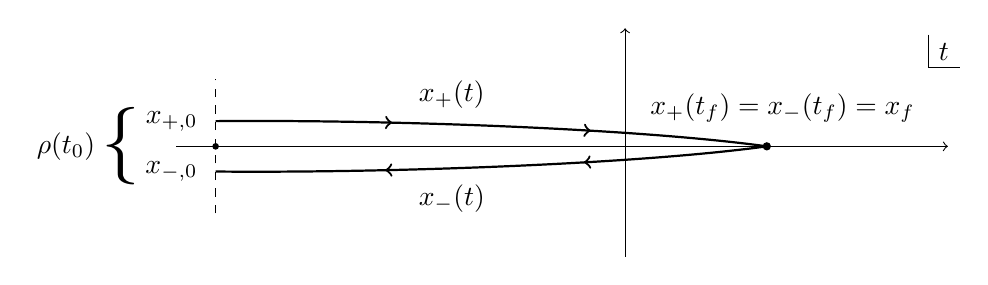
\begin{tikzpicture}[
    x=1cm,
    y=1cm,
    contour/.style={
        thick,
        postaction={decorate}
    },
    forward/.style={
        contour,
        decoration={
            markings,
            mark=at position 0.32 with {\arrow{>}},
            mark=at position 0.68 with {\arrow{>}}
        }
    },
    backward/.style={
        contour,
        decoration={
            markings,
            mark=at position 0.32 with {\arrow{<}},
            mark=at position 0.68 with {\arrow{<}}
        }
    }
]


\draw[->] (-0.5,0) -- (9.3,0);
\draw[->] (5.2,-1.4) -- (5.2,1.5);


\draw (8.05+1,1.42) -- (8.05+1,1.00) -- (8.45+1,1.00);
\node at (9.25,1.20) {$t$};


\draw[dashed] (0,-0.85) -- (0,0.85);


\fill (0,0) circle (1.2pt);



\node at (-1.9,0) {$\rho(t_0)$};
\node[scale=2.8] at (-1.2,0) {$\{$};


\node[left=3pt] at (0,0.32) {$x_{+,0}$};
\node[left=3pt] at (0,-0.32) {$x_{-,0}$};



\draw[forward]
    (0,0.32)
    .. controls (2.3,0.34) and (5.4,0.22) ..
    (7,0);


\draw[backward]
    (0,-0.32)
    .. controls (2.3,-0.34) and (5.4,-0.22) ..
    (7,0);


\node[above=2pt] at (3.0,0.29) {$x_+(t)$};
\node[below=2pt] at (3.0,-0.29) {$x_-(t)$};








\fill (7,0) circle (1.5pt);

\node[above=5pt, anchor=south] at (7.2,0)
    {$x_+(t_{f})=x_-(t_{f})=x_f$};
    
\end{tikzpicture}


\caption{複素$ t$平面上のSK経路。$ \rho(t_{0})$の後の括弧は、経路積分の境界条件$ x_{\pm,0}$を初期密度行列で平均すべきことを示す。見やすくするため、順方向と逆方向の経路を虚方向にわずかに離して描いている。\label{fig:SK}}
\end{figure}






\paragraph{閉時間経路} 経路積分の役割は、経路順序付き相関関数を計算することである。振幅の計算で用いるin-out相関関数の経路積分のように、経路が時間方向へ一直線に進むなら、経路順序と時間順序は一致する。SK経路積分のように、経路が折り返して時間を戻るなら、\textit{経路順序}と\textit{時間順序}は異なる。順方向の枝では経路順序は通常の時間順序と一致し、逆方向の枝では反時間順序と一致する。それぞれの枝に一つずつ挿入がある場合、それらの間には通常の時間順序はなく、経路そのものが順序を決める。



この区別を明確にするため、SK経路積分の二つの枝を、\textit{閉時間経路}と呼ばれる一つの経路の二つの部分と考えると便利なことがある。これは、順方向と逆方向の枝が、折り返し点$ t_{f}$で正則性条件$ x_{+}(t_{f})=x_{-}(t_{f})$によってつなぎ合わされるため可能である。言い換えると、トレースが時間方向に経路を閉じる。実際、二枝の経路積分を、一つの経路積分
\begin{align}
\int_{\rm I.C.}\mathcal D x_+\,
\int_{\rm I.C.}\mathcal D x_- \to \int_{\rm I.C.}^{\rm I.C.}\mathcal{D}X
\end{align}
として書き直せる。ここで$ X(\lambda)$は$ x_{+}$と$ x_{-}$の両方を含む新しい積分変数で、$  \lambda$は時間に関係する経路変数である。より具体的には、折り返し点が$ t_{f}=0\geq t_{0}$となり、すべての演算子挿入がそれ以前にあるように時刻をずらすと、$ t_{0}\leq \lambda \leq |t_{0}|$となり、次のように同定できる。
\begin{equation}
\begin{cases}
X(\lambda)=x_{+}(\lambda) \text{ ただし } t_{0}\leq \lambda \leq 0  \\
X(\lambda)=x_{-}(-\lambda) \text{ ただし } 0 \leq \lambda \leq |t_{0}| \,.
\end{cases}
\end{equation}
変数$ X(\lambda)$についての経路順序は通常のものであり、早い$ \lambda_{1}$での挿入は、遅い$ \lambda_{2}> \lambda_{1}$での挿入の右側に来る。この単純な$ \lambda$の経路順序から、多様な時間順序が生じる。\\





具体例で見てみよう。二点関数については、
\begin{align}\label{++}
\langle\!\langle x_+(t)\,x_+(t')\rangle\!\rangle
&=
\langle T\,x(t)x(t')\rangle ,
\\
\langle\!\langle x_-(t)\,x_-(t')\rangle\!\rangle
&=
\langle \bar T\,x(t)x(t')\rangle ,
\\
\langle\!\langle x_+(t)\,x_-(t')\rangle\!\rangle
&=
\langle x(t')x(t)\rangle ,
\\
\langle\!\langle x_-(t)\,x_+(t')\rangle\!\rangle
&=
\langle x(t)x(t')\rangle .
\end{align}
となる。したがって、$+$枝上の場同士は時間順序付けされ、$-$枝上の場同士は反時間順序付けされる。異なる枝の場は、しばしばWightman相関関数と呼ばれる、時間順序のない相関関数を与える。例として、\eqref{++}の図式的表現を図\ref{fig:SKinsertion}に示す。



より一般には、プラス枝とマイナス枝の任意個数の演算子の平均を考えられる。これは、時間順序付きのブロックと反時間順序付きのブロックの積を与える。
\begin{align}
\expi{\prod_{i=1}^{n}\O_{+}(t_{i})\prod_{j=1}^{m}\O_{-}(t_{j})}=\ex{\bar T \left[ \prod_{j=1}^{m}\O(t_{j}) \right] T \left[ \prod_{i=1}^{n}\O(t_{i}) \right]}\,.
\end{align}
さらに一般には、任意の順序\cite{Aleiner:2016eni,Haehl:2017qfl}にある演算子の相関関数を計算したい場合がある。これらは非時間順序相関関数（Out-of-Time-Order Correlators、OTOC）と呼ばれることがあり、量子カオスの診断法として近年注目されている。このような一般的な順序は、逆方向と順方向の発展を交互に繰り返す枝を増やしたSK経路積分の一般化によって計算できる。ただし、各枝は前後の枝と連続的につなぎ合わされる。



\begin{figure}
\centering



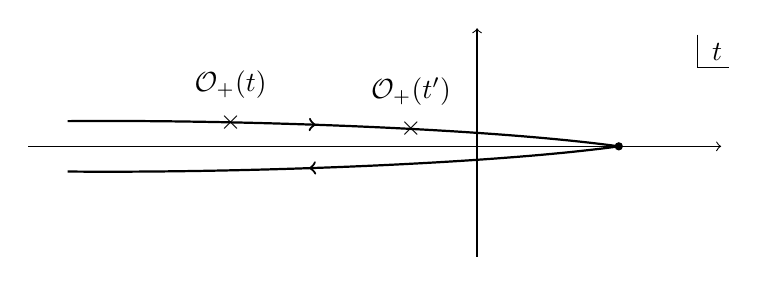
\begin{tikzpicture}[
    x=1cm,
    y=1cm,
    contour/.style={
        thick,
        postaction={decorate}
    },
    forward/.style={
        contour,
        decoration={
            markings,
            mark=at position 0.45 with {\arrow{>}}
        }
    },
    backward/.style={
        contour,
        decoration={
            markings,
            mark=at position 0.45 with {\arrow{<}}
        }
    }
]


\draw[->] (-0.5,0) -- (8.3,0);
\draw[->] (5.2,-1.4) -- (5.2,1.5);


\draw (8.0,1.42) -- (8.0,1.00) -- (8.4,1.00);
\node at (8.25,1.20) {$t$};





\draw[forward]
    (0,0.32)
    .. controls (2.3,0.34) and (5.4,0.22) ..
    coordinate[pos=0.28] (opA)
    coordinate[pos=0.58] (opB)
    (7,0);


\draw[backward]
    (0,-0.32)
    .. controls (2.3,-0.34) and (5.4,-0.22) ..
    (7,0);


\fill (7,0) circle (1.5pt);


\node at (opA) {$\times$};
\node[above=5pt] at (opA) {$\mathcal{O}_{+}(t)$};

\node at (opB) {$\times$};
\node[above=5pt] at (opB) {$\mathcal{O}_{+}(t')$};

\end{tikzpicture}


\caption{時間順序付き二点関数に対応する、プラス枝上の二つの演算子挿入を含むSK経路。見やすさのため、図\ref{fig:SK}のラベルはすべて省略している。\label{fig:SKinsertion}}
\end{figure}






\paragraph{遅延・先進基底} ここで\textit{Keldysh基底}を導入する。
\begin{equation}
x_r := \frac{x_+ + x_-}{2},
\qquad
x_a := x_+ - x_- ,
\end{equation}
逆の関係は
\begin{equation}
x_+ = x_r + \frac{x_a}{2},
\qquad
x_- = x_r - \frac{x_a}{2} .
\end{equation}
である。変数$x_r$は二つの経路コピーの平均であり、\textit{遅延}成分と呼ばれることが多い。変数$x_a$はその差であり、\textit{先進}成分と呼ばれることが多い。これらが、どのように、またどのような場合に古典的・量子的な寄与と関係するかをまもなく論じるが、本ノートではその呼び方を避ける。この基底では、先に論じた非平衡の制約が特に簡単な形を取り、揺らぎと応答の区別がはるかに明瞭になる。



$r/a$基底の二点関数は、$\pm$の相関関数の単純な線形結合から得られる。まず、
\begin{align}
\langle\!\langle x_r(t)x_r(t^{\prime})\rangle\!\rangle
&=
\frac{1}{4}
\langle\!\langle
\bigl(x_+(t)+x_-(t)\bigr)
\bigl(x_+(t^{\prime})+x_-(t^{\prime})\bigr)
\rangle\!\rangle
\nonumber\\
&=
\frac{1}{4}
\Bigl[
\langle\!\langle x_+(t)x_+(t^{\prime})\rangle\!\rangle
+
\langle\!\langle x_+(t)x_-(t^{\prime})\rangle\!\rangle
\nonumber\\
&\hspace{1.5cm}
+
\langle\!\langle x_-(t)x_+(t^{\prime})\rangle\!\rangle
+
\langle\!\langle x_-(t)x_-(t^{\prime})\rangle\!\rangle
\Bigr]
\nonumber\\
&=
\frac{1}{4}
\Bigl[
\langle  T\,\hat x(t)\hat x(t^{\prime})\rangle
+
\langle \hat x(t^{\prime})\hat x(t)\rangle
\nonumber\\
&\hspace{1.5cm}
+
\langle \hat x(t)\hat x(t^{\prime})\rangle
+
\langle \widetilde{ T}\,\hat x(t)\hat x(t^{\prime})\rangle
\Bigr]
\nonumber\\
&=
\frac{1}{4}
\Bigl[
\theta(t-t^{\prime})
\langle \hat x(t)\hat x(t^{\prime})\rangle
+
\theta(t^{\prime}-t)
\langle \hat x(t^{\prime})\hat x(t)\rangle
\nonumber\\
&\hspace{1.5cm}
+
\langle \hat x(t^{\prime})\hat x(t)\rangle
+
\langle \hat x(t)\hat x(t^{\prime})\rangle
\nonumber\\
&\hspace{1.5cm}
+
\theta(t^{\prime}-t)
\langle \hat x(t)\hat x(t^{\prime})\rangle
+
\theta(t-t^{\prime})
\langle \hat x(t^{\prime})\hat x(t)\rangle
\Bigr]
\nonumber\\
&=
\frac{1}{2}
\Bigl[
\langle \hat x(t)\hat x(t^{\prime})\rangle
+
\langle \hat x(t^{\prime})\hat x(t)\rangle
\Bigr]=
\frac{1}{2}
\langle
\{\hat x(t),\hat x(t^{\prime})\}
\rangle .
\end{align}














すなわち、場の反交換子である。これは対称化された相関関数、あるいは\textit{Keldysh相関関数}である。次に、他の二点関数も同様に計算できる。途中の計算は読者の演習として、次を得る。
\begin{align}
\langle\!\langle x_r(t)x_a(t')\rangle\!\rangle
&=
\frac12
\langle\!\langle
\bigl(x_+(t)+x_-(t)\bigr)
\bigl(x_+(t')-x_-(t')\bigr)
\rangle\!\rangle
\nonumber\\
&=
\theta(t-t')\,\langle [\hat x(t),\hat x(t')]\rangle .
\end{align}
これは、場の理論で慣習的に含めることが多い因子$-i$を除けば、遅延相関関数である。同様に、
\begin{align}
\langle\!\langle x_a(t)x_r(t')\rangle\!\rangle
&=
\frac12
\langle\!\langle
\bigl(x_+(t)-x_-(t)\bigr)
\bigl(x_+(t')+x_-(t')\bigr)
\rangle\!\rangle
\nonumber\\
&=
\theta(t'-t)\,\langle [\hat x(t'),\hat x(t)]\rangle ,
\end{align}
となり、これが先進相関関数である。Heavisideの階段関数は、先進変数に現れる時刻を常に遅延変数の時刻より前に置く。このことが、それらの名称を正当化している。最後に、









\begin{align}
    \expi{x_{a}(t)x_{a}(t')}&= \expi{\left[ x_{+}(t)-x_{-}(t) \right] \left[ x_{+}(t')-x_{-}(t') \right]}\\
    &=\ex{T \hat x(t)\hat x(t')}+\ex{\widetilde T \hat x(t)\hat x(t')}-\ex{  \hat x(t)\hat x(t')}-\ex{  \hat x(t')\hat x(t)}=0\,.
\end{align}
である。したがって、$r/a$基底での四つの基本的な二点関数は、
\begin{align}
G_K(t,t') := \langle\!\langle x_r(t)x_r(t')\rangle\!\rangle
&= \frac12\langle \{\hat x(t),\hat x(t')\}\rangle ,
\\
G_R(t,t') := \langle\!\langle x_r(t)x_a(t')\rangle\!\rangle
&= \theta(t-t')\langle [\hat x(t),\hat x(t')]\rangle ,
\\
G_A(t,t') := \langle\!\langle x_a(t)x_r(t')\rangle\!\rangle
&= \theta(t'-t)\langle [\hat x(t'),\hat x(t)]\rangle ,
\\
\langle\!\langle x_a(t)x_a(t')\rangle\!\rangle &=0 .
\end{align}
となる。これらはそれぞれ、Keldysh伝播子、遅延伝播子、先進伝播子、恒等的にゼロの$aa$伝播子である。これは$r/a$基底が非常に有用である主な理由の一つだ。応答関数はHeaviside関数を掛けた交換子として直ちに同定され、揺らぎは対称化された相関関数によって捉えられる。



遅延場と先進場の積の経路積分期待値を計算するには、二つの枝に結合するソース\(J_\pm\)を、そのKeldysh結合
\begin{equation}\label{Jra}
J_r := \frac{J_+ + J_-}{2},
\qquad
J_a := J_+ - J_- ,
\end{equation}
あるいは等価に、
\begin{equation}
J_+ = J_r + \frac{J_a}{2},
\qquad
J_- = J_r - \frac{J_a}{2} .
\end{equation}
で置き換えると便利である。ここで\(J_r\)を遅延ソース、または平均ソース、\(J_a\)を先進ソース、または差ソースと呼ぶ。Keldysh基底では、ソース項は
\begin{equation}
J_+x_+ - J_-x_-
=
J_a x_r + J_r x_a ,
\end{equation}
となり、Schwinger--Keldysh生成汎関数は
\begin{equation}
Z[J_r,J_a]
=
\int \mathcal D x_r\,\mathcal D x_a\;
\exp\!\left(
iS_{\rm SK}[x_r,x_a]
+
i\int dt\,\bigl(J_a x_r + J_r x_a\bigr)
\right) .
\end{equation}
と書ける。\eqref{Jra}という合理的な規約の、少々紛らわしい帰結は、\(x_r\)の挿入が\(J_a\)に関する微分で生成され、\(x_a\)の挿入が\(J_r\)に関する微分で生成されることである。



$aa$二点関数がゼロになることは偶然ではない。より一般に、先進場だけで構成された相関関数はゼロになる。
\begin{equation}\label{aeq0}
\langle\!\langle x_a(t_1)\cdots x_a(t_n)\rangle\!\rangle = 0
\qquad
\text{任意の } n\geq 1 .
\end{equation}
これは、Schwinger--Keldysh生成汎関数の規格化条件から直接従う\footnote{別の導出では、関係$x_a=x_+ -x_-$を用いる。\(n\)個の先進場の積を展開すると、各挿入を順方向または逆方向の枝に割り当てる\(2^n\)通りのすべてについての、符号付きの和となる。このとき結果\eqref{aeq0}は、経路順序付き相関関数の交代和が消えるという恒等式と等価である。
\begin{equation}
\expi {\prod_{m=1}^n x_a(t_m) }
=
\sum_{I\subseteq \{1,\dots,n\}}
(-1)^{\,n-|I|}
\left\langle
\bar T \prod_{j\notin I}\hat x(t_j)\;
T \prod_{i\in I}\hat x(t_i)
\right\rangle
=0 .
\end{equation}
}。\(r/a\)基底では、
\[Z[J_r,J_a=0]=1 \]
が任意の\(J_r\)に対して成り立つ。\(x_a\)の挿入は\(J_r\)に関する微分で生成されるため、\eqref{aeq0}が直ちに従う。



高次では、$r/a$基底は相関関数を入れ子の交換子へと整理する。最も重要な一般的な族は、一つの$r$挿入と任意個数の$a$挿入から得られる。これらが高次の遅延相関関数である。時刻が
\begin{equation}
t_1>t_2>\cdots>t_n ,
\end{equation}
の順に並ぶ場合、
\begin{equation}\label{higherretarded}
\langle\!\langle x_r(t_1)x_a(t_2)\cdots x_a(t_n)\rangle\!\rangle
=
\left\langle
[\cdots[[\hat x(t_1),\hat x(t_2)],\hat x(t_3)]\cdots,\hat x(t_n)]
\right\rangle ,
\end{equation}
を得る。任意の時刻引数に対しては、遅延的な台を課すHeaviside関数の適切な積を加えて、
\begin{align}
\langle\!\langle x_r(t_1)x_a(t_2)\cdots x_a(t_n)\rangle\!\rangle
&=
\theta(t_1-t_2)\theta(t_2-t_3)\cdots\theta(t_{n-1}-t_n)
\nonumber\\
&\qquad\times
\left\langle
[\cdots[[\hat x(t_1),\hat x(t_2)],\hat x(t_3)]\cdots,\hat x(t_n)]
\right\rangle
\;+\; \text{置換による項} .
\end{align}
とする。このように、$a$挿入を一つ追加するごとに、交換子の入れ子が一段深くなる。これが、先進場が応答場であることの正確な意味である。$  J_{r} $に関する微分が応答関数を生成するのである。



まとめると、$\pm$基底は経路構造を明示する。順方向の枝の時間順序、逆方向の枝の反時間順序、枝をまたぐWightman関数を直接符号化する。一方、$r/a$基底は応答と揺らぎを明示する。$rr$相関関数は対称化された二点関数を与え、$ra$と$ar$の相関関数は遅延・先進伝播子を与える。$a$場だけで構成された相関関数は恒等的にゼロになる。





\subsection{環境の積分消去とFeynman--Vernon影響汎関数}



ここで閉鎖系から開放系へ、すなわちHamilton的な発展から一般に非Hamilton的な発展へ進む。概念上の出発点は依然として完全にHamilton的な理論だが、今度は全Hilbert空間を、関心のある部分系$ S$と環境$ E$に分ける。
\begin{equation}
\mathcal H = \mathcal H_S \otimes \mathcal H_E .
\end{equation}
系の自由度を\(x\)、環境の自由度を\(q\)と表す。一般性を失わず、全作用も対応して次のように分解する。
\begin{equation}
S_{\rm tot}[x,q]
=
S_S[x] + S_E[q] + S_{\rm int}[x,q] .
\end{equation}
この段階では、完全な理論は依然として閉じており、あるHamiltonianに従ってユニタリに発展する。



したがって、全体系のSchwinger--Keldysh生成汎関数$  Z[J_+,J_-] $は
\begin{align}
&Z=\int dx_{+,0}\,dx_{-,0}\,dq_{+,0}\,dq_{-,0}\,dx_f\,dq_f\;
\rho_{SE}(x_{+,0},q_{+,0};x_{-,0},q_{-,0};t_0)
\nonumber\\
& \int_{x_+(t_0)=x_{+,0},\,q_+(t_0)=q_{+,0}}^{x_+(t_f)=x_f,\,q_+(t_f)=q_f}
\mathcal D x_+\,\mathcal D q_+ 
\exp\!\Bigl[
iS_S[x_+] + iS_E[q_+] + iS_{\rm int}[x_+,q_+]
+ i\int dt J_+x_+
\Bigr]
\nonumber\\
&  \int_{x_-(t_0)=x_{-,0},\,q_-(t_0)=q_{-,0}}^{x_-(t_f)=x_f,\,q_-(t_f)=q_f}
\mathcal D x_-\,\mathcal D q_- 
\exp\!\Bigl[
-iS_S[x_-] - iS_E[q_-] - iS_{\rm int}[x_-,q_-]
- i\int dt J_-x_-
\Bigr] .\nonumber
\end{align}
である。先ほどと同様に、式が過度に大きくなるのを避けるため、以下では経路積分の上端の境界値を省略し、プラス枝とマイナス枝の間で常に連続であることを暗黙に了解する。また、経路積分の可能なすべての下端境界条件について、密度行列$ \rho$による重みで平均すべきことを表すため、略記$ \int_{\rho}$を用いる。こうして、より簡潔に
\begin{align}
Z[J_+,J_-]
&=
\int_{\rho_{SE}(t_0)} \mathcal D x_+\,\mathcal D x_-\,\mathcal D q_+\,\mathcal D q_-\;
\exp\Bigl(
iS_S[x_+] - iS_S[x_-]
+iS_E[q_+] - iS_E[q_-]
\nonumber\\
&\hspace{1.5cm}
+iS_{\rm int}[x_+,q_+] - iS_{\rm int}[x_-,q_-]
+i\int dt\,J_+ x_+ - i\int dt\,J_- x_-
\Bigr) .
\end{align}


と書く。ここで\(\rho_{SE}(t_0)\)は全体系の初期密度行列である。最も簡単で一般的な設定では、初期状態が因子化していると仮定する。
\begin{equation}\label{factorisedrho}
\rho_{SE}(t_0)=\rho_S(t_0)\otimes \rho_E(t_0) ,
\end{equation}
ただし、以下の形式的な操作は一般化できる。



ここで重要な段階は、環境変数\(q_\pm\)を積分消去することである。これによって、Feynman--Vernonの\textit{影響汎関数}\footnote{Feynman--Vernon影響\textit{汎関数}という語を$ e^{iS_{\mathrm{IF}}}$に用い、$S_{\mathrm{IF}}$を影響\textit{作用}と呼ぶこともある。本ノートではこの区別をしない。}\cite{FEYNMAN1963118}が定義される。具体的には、次を定義する。
\begin{align}
e^{\,iS_{\rm IF}[x_+,x_-]}
&:=
\int_{\rho_{E}(t_{0})} \mathcal D q_+\,\mathcal D q_-\;
\exp\Bigl(
iS_E[q_+] - iS_E[q_-]
+iS_{\rm int}[x_+,q_+]
-iS_{\rm int}[x_-,q_-]
\Bigr)\,.
\end{align}
この対象は、系の履歴\(x_+\)と\(x_-\)だけに依存するが、環境が部分系に与える効果をすべて含む。次の小節で見るように、影響汎関数は、系の二つの異なる履歴のもとで発展した、二つの環境状態間の重なり振幅として書ける。
この定義を行うと、生成汎関数は
\begin{align}
Z[J_+,J_-]
&=
\int \mathcal D x_+\,\mathcal D x_-\;
\exp\Bigl(
iS_S[x_+] - iS_S[x_-]
+iS_{\rm IF}[x_+,x_-]
+i\int dt\,J_+x_+
-i\int dt\,J_-x_-
\Bigr)
\nonumber\\
&\hspace{2.3cm}
\times
\rho_S(x_{+,0},x_{-,0};t_0) .
\end{align}
となる。したがって、開放系の有効作用を次のように定義するのが自然である。
\begin{equation}
S_{\rm eff}[x_+,x_-]
:=
S_S[x_+] - S_S[x_-] + S_{\rm IF}[x_+,x_-] .
\end{equation}


これが中心的な結果である。閉鎖系ではSchwinger--Keldysh作用は単に差\(S[x_+]-S[x_-]\)である。開放系では、環境を積分消去すると追加の項\(S_{\rm IF}[x_+,x_-]\)が生成され、これは一般に経路の二つの枝を結合する。これらの枝を混合する項には、純粋にHamilton的な閉鎖系の発展に対応物がなく、環境が縮約動力学に及ぼす効果を符号化しているのが、まさにそれらの項である。



影響汎関数には明確な物理的意味がある。環境を介したすべての効果を、\(x_+\)と\(x_-\)の一つの汎関数にまとめるのである。問題に応じて、系のパラメータのシフト、散逸、確率的揺らぎ、記憶効果などが含まれる。一般に、\(S_{\rm IF}\)は時間について非局所的である。環境は系の過去の履歴の一部を記憶するため、縮約動力学は非Markov的になる。この意味で、Feynman--Vernon形式は、Markov近似を行う前の、開放量子動力学の厳密な実時間記述を与える。第\ref{sec:4p7}節では、簡単な設定で影響汎関数を具体的に計算する。



直ちにKeldysh基底へ移ると便利な場合が多い。
\begin{equation}
x_r := \frac{x_+ + x_-}{2},
\qquad
x_a := x_+ - x_- .
\end{equation}
このとき影響汎関数は\(S_{\rm IF}[x_r,x_a]\)となり、まもなく見るように、その構造をより直接的に解釈できる。





\subsection{Schwinger--Keldysh有効作用の制約}



具体例を調べる前に、密度行列の時間発展を記述するために、任意のSchwinger--Keldysh有効作用が満たすべき一般的な制約を理解することが重要である。これらの制約は、密度行列を定義する性質
\begin{equation}
\Tr \rho = 1,
\qquad
\rho^\dagger = \rho,
\qquad
\rho \ge 0 .
\end{equation}
から直接従う。これらは、トレース保存性、Hermite性の保存、正値性に対応する経路積分版である。より強い要請である完全正値性は、次の小節へ先送りする。本小節では、それらに対応する有効作用の条件、すなわち
\begin{equation}
S_{\rm eff}[x_+,x_+]=0,
\qquad
S_{\rm eff}[x_+,x_-]= -\,S_{\rm eff}^*[x_-,x_+],
\qquad
\Im S_{\rm eff}[x_+,x_-]\geq 0 .
\end{equation}
を導く。Hamilton的な発展では、\(S_{\rm eff}=S[x_+]-S[x_-]\)であり、ユニタリ性により\(S\)がその変数の実汎関数となるため、これらの制約は自明に満たされる。非自明なのは、影響汎関数$  S_{\rm IF} $もこれらの条件を満たすことであり、以下ではこれに注目する。




証明の論理は次のとおりである。関心のある部分系\(x\)と環境\(q\)からなる全体系のユニタリ発展から出発し、\(x_+\)と\(x_-\)を外部ソースとして扱って発展させた、二つの環境状態の重なりとして影響汎関数を書き直す。この形では、標準的なSchwinger--Keldyshの制約がほぼ直ちに従う。この導出は、文献\cite{Glorioso:2016gsa,Salcedo:2024smn}の付録Aを直接的に応用したものである。



\eqref{factorisedrho}のように初期密度行列が因子化していると仮定すると、影響汎関数は
\begin{equation}
e^{\,iS_{\rm IF}[x_+,x_-]}
=
\int dq\,dq_i\,dq_i'\;
\int_{q_i}^{q}\mathcal D q_+\;
\int_{q_i'}^{q}\mathcal D q_-\;
e^{\,iS_{\rm tot}[x_+,q_+] - iS_{\rm tot}[x_-,q_-]}\,
\rho_q^{(0)}(q_i,q_i') .
\end{equation}
となる。ここで重要なのは、\(x_+\)と\(x_-\)を環境に対する外部ソースとみなすことである。指定された背景履歴\(x_+\)のもとでの環境の時間発展演算子を\(U_q(t,t_0;\{x_+\})\)と表し、\(x_-\)についても同様にすると、二つの環境経路積分を、ソース付き時間発展演算子の行列要素として書き直せる。
\begin{equation}
\int_{q_i}^{q}\mathcal D q_+\; e^{\,iS_{\rm tot}[x_+,q_+]}
=
\langle q|\,U_q(t,t_0;\{x_+\})\,|q_i\rangle ,
\end{equation}
\begin{equation}
\int_{q_i'}^{q}\mathcal D q_-\; e^{-\,iS_{\rm tot}[x_-,q_-]}
=
\Bigl[\langle q|\,U_q(t,t_0;\{x_-\})\,|q_i'\rangle\Bigr]^\dagger .
\end{equation}
議論をできるだけ簡単にするため、以下では環境が初めに純粋状態
\[   \rho_q^{(0)}(q_i,q_i') =  \ket{\Omega_q}\bra{\Omega_q}. \]
にあると仮定する。上の表式を影響汎関数に代入し、環境Hilbert空間の恒等演算子を挿入すると、
\begin{equation}
e^{\,iS_{\rm IF}[x_+,x_-]}
=
\langle \Omega_q|\,
U_q^\dagger(t,t_0;\{x_-\})\,
U_q(t,t_0;\{x_+\})\,
|\Omega_q\rangle .
\end{equation}
を得る。等価に、ソースのもとで発展した環境状態を
\begin{equation}
|\Omega_q^{\{x_+\}}(t)\rangle
:=
U_q(t,t_0;\{x_+\})\,|\Omega_q\rangle ,
\qquad
\langle \Omega_q^{\{x_-\}}(t)|
:=
\langle\Omega_q|\,U_q^\dagger(t,t_0;\{x_-\}) ,
\end{equation}
と定義すれば、簡潔な表式
\begin{equation}\label{eq:influence-overlap}
e^{\,iS_{\rm IF}[x_+,x_-]}
=
\langle \Omega_q^{\{x_-\}}(t)\,|\,\Omega_q^{\{x_+\}}(t)\rangle .
\end{equation}
を得る。したがって、影響汎関数は、系の二つの異なる履歴のもとで発展した二つの環境状態の重なり振幅である。これが、制約を導く鍵となる結果である。



第一の帰結は、虚部の正値性である。\eqref{eq:influence-overlap}の状態は規格化されているため、Cauchy--Schwarzの不等式から
\begin{equation}
\bigl|e^{\,iS_{\rm IF}[x_+,x_-]}\bigr|
=
\bigl|\langle \Omega_q^{\{x_-\}}(t)\,|\,\Omega_q^{\{x_+\}}(t)\rangle\bigr|
\le 1 .
\end{equation}
が従う。よって、
\begin{equation}
e^{-\Im S_{\rm IF}[x_+,x_-]} \le 1  \then 
\Im S_{\rm IR}[x_+,x_-] \ge 0 .
\end{equation}
である。これが、正値性の制約の経路積分での形である。



第二の帰結はHermite性である。\eqref{eq:influence-overlap}の複素共役を取ると、
\begin{equation}
e^{-\,iS_{\rm IF}^*[x_+,x_-]}
=
\langle \Omega_q^{\{x_+\}}(t)\,|\,\Omega_q^{\{x_-\}}(t)\rangle
=
e^{\,iS_{\rm IF}[x_-,x_+]} ,
\end{equation}
を得る。したがって、
\begin{equation}
S_{\rm IF}[x_+,x_-]
=
-\,S_{\rm IF}^*[x_-,x_+] .
\end{equation}
となる。これが、縮約密度行列のHermite性から従うSchwinger--Keldyshの実条件である。



第三の帰結は、規格化、すなわちトレース保存の条件である。二つの履歴が\(x_+=x_-\)と一致すれば、環境の二つのソース付き発展は同一となり、\eqref{eq:influence-overlap}は単一の状態のノルムに帰着する。
\begin{equation}
e^{\,iS_{\rm IF}[x_+,x_+]}
=
\langle \Omega_q^{\{x_+\}}(t)\,|\,\Omega_q^{\{x_+\}}(t)\rangle
=
1 .
\end{equation}
よって、
\begin{equation}
S_{\rm IF}[x_+,x_+] = 0 .
\end{equation}
となる。これが、二つの枝を同一視するとSchwinger--Keldysh有効作用がゼロになる、という主張の正確な導出である。



Keldysh基底へ移り、$  S_{\rm IF} $と発展のHamilton的な部分を合わせて完全なSK作用$  S_{\rm eff} $を作ると、これらの制約は
\begin{align}\label{constraintsra}
S_{\rm eff}[x_r,x_a=0] &= 0 ,\\
S_{\rm eff}[x_r,x_a] &= -\,S_{\rm eff}^*[x_r,-x_a] ,\\
\Im S_{\rm eff}[x_r,x_a] &\ge 0 .
\end{align}
となる。これらは非摂動的に成り立ち、完全な理論の基礎にあるHamilton的発展から直接受け継がれる。任意のSchwinger--Keldysh有効作用に対する基本的なユニタリ性の制約であり、非平衡の制約とも呼ばれる。長くはなるが、より正確な名称は「全体系のユニタリ性からの制約」だろう。これは、これらが破られる場合、仮定\eqref{factorisedrho}のもとでは、ユニタリな全体系から環境を積分消去することで、その開放系動力学を得ることはできない、という事実を強調する。






\subsection{系に線形結合したガウス的環境}\label{sec:4p7}



ここでは、影響汎関数を厳密に計算できる具体的なモデルを論じる。この例の目的は、環境の積分消去によって系の非自明なSchwinger--Keldysh有効作用がどう生成され、特徴的な枝を混合する構造がどう生じるかを、具体的な設定で示すことである。ガウス場\(q\)で記述される環境に線形結合した、系の自由度\(x\)を考える。



全作用を
\begin{equation}
S_{\rm tot}[x,q]
=
S_S[x]+S_E[q]+S_{\rm int}[x,q] ,
\end{equation}
とし、相互作用を
\begin{equation}
S_{\rm int}[x,q]
=
\int dt\, g\,x(t)\,q(t) .
\end{equation}
とする。具体的には、\(q\)を単一の調和振動子、あるいはより一般に調和振動子の集合と考えてよい。本質的な仮定は、環境作用\(S_E[q]\)が\(q\)について二次であり、そのため\(q\)の経路積分がガウス型となって厳密に実行できることである。



Schwinger--Keldysh形式では、相互作用項は
\begin{equation}
S_{\rm int}[x_+,q_+]-S_{\rm int}[x_-,q_-]
=
g\int dt\,\bigl(x_+(t)q_+(t)-x_-(t)q_-(t)\bigr) .
\end{equation}
となる。したがって、影響汎関数は
\begin{align}
e^{\,iS_{\rm IF}[x_+,x_-]}
&=
\int_{\rho_E(t_0)} \mathcal D q_+\,\mathcal D q_-\;
\exp\Biggl\{
iS_E[q_+]-iS_E[q_-]
\nonumber\\
&\hspace{2cm}
+i g\int dt\,\bigl(x_+(t)q_+(t)-x_-(t)q_-(t)\bigr)
\Biggr\} .
\end{align}
である。環境がガウス的なので、これは線形ソースをもつガウス汎関数積分であり、平方完成によって厳密に評価できる。結果は系の履歴\(x_+\)と\(x_-\)について二次となる。
\begin{align}\label{IFpmGaussian}
S_{\rm IF}[x_+,x_-]
=
i\frac{g^2}{2}
\int dt\,dt'\,
\Big[
x_+(t)\,G_{++}(t,t')\,x_+(t')
-x_+(t)\,G_{+-}(t,t')\,x_-(t')
\nonumber\\
\hspace{3.7cm}
-x_-(t)\,G_{-+}(t,t')\,x_+(t')
+x_-(t)\,G_{--}(t,t')\,x_-(t')
\Big] ,
\end{align}
ここで\(a,b\in\{+,-\}\)に対する\(G_{ab}(t,t')\)は、環境演算子\(q\)のSchwinger--Keldysh二点関数である。
\begin{align}
G_{++}(t,t')
&:=
\langle\!\langle q_+(t)q_+(t')\rangle\!\rangle
=
\langle T\,\hat q(t)\hat q(t')\rangle ,
\\
G_{+-}(t,t')
&:=
\langle\!\langle q_+(t)q_-(t')\rangle\!\rangle
=
\langle \hat q(t')\hat q(t)\rangle ,
\\
G_{-+}(t,t')
&:=
\langle\!\langle q_-(t)q_+(t')\rangle\!\rangle
=
\langle \hat q(t)\hat q(t')\rangle ,
\\
G_{--}(t,t')
&:=
\langle\!\langle q_-(t)q_-(t')\rangle\!\rangle
=
\langle \bar T\,\hat q(t)\hat q(t')\rangle .
\end{align}
言い換えると、厳密な影響汎関数は、環境の二点相関関数によって完全に決まる。これは、系に線形結合したガウス的環境が二次の影響汎関数を生むという一般的事実を、最も簡単に具体化した例である。\\



ここでKeldysh基底に移ると有用である。いくらか計算すると、影響汎関数は標準的な形
\begin{align}\label{IFraGaussian}
S_{\rm IF}[x_r,x_a]
=
- g^2\int dt\,dt'\,
x_a(t)\,D_R(t,t')\,x_r(t')
+\frac{i g^2}{2}\int dt\,dt'\,
x_a(t)\,N(t,t')\,x_a(t') .
\end{align}
を取る。\(D_R\)と\(N\)を\(q\)の相関関数で表す前に、すでにいくつかの性質が分かる。第一に、\(N(t,t')\)の反対称部分は\eqref{IFraGaussian}に寄与しない。第二に、
\begin{equation}
D_R(t,t')
=
D_R^{(S)}(t,t')+D_R^{(A)}(t,t'),
\end{equation}
と分解できる。ここで
\begin{equation}
D_R^{(S)}(t,t')=D_R^{(S)}(t',t),
\qquad
D_R^{(A)}(t,t')=-D_R^{(A)}(t',t).
\end{equation}
である。\(x_a=x_+-x_-\)と\(x_r=(x_++x_-)/2\)を用いると、対称部分の寄与は
\begin{align}
\int dt\,dt'\,
x_a(t)D_R^{(S)}(t,t')x_r(t')
&=
\frac{1}{2}\int dt\,dt'\,
\left[
x_+(t)D_R^{(S)}(t,t')x_+(t')
-
x_-(t)D_R^{(S)}(t,t')x_-(t')
\right]. \nonumber
\end{align}
となる。\(D_R^{(S)}\)が対称なので、混合した$ +  $／$ -  $の項は打ち消し合う。したがって、この寄与は
\begin{equation}
S_{\rm cons}[x_+]-S_{\rm cons}[x_-],
\end{equation}
の形となり、系の保存的な作用の再定義へ吸収できる。



対照的に、\(D_R^{(A)}\)を含む対角項は消え、混合項は加わる。
\begin{align}
- g^2\int dt\,dt'\,
x_a(t)D_R^{(A)}(t,t')x_r(t')
&=
- g^2\int dt\,dt'\,
x_+(t)D_R^{(A)}(t,t')x_-(t').
\end{align}
この項はSchwinger--Keldysh経路の二つの枝を結合し、単一枝の作用二つの差としては書けない。したがって、影響汎関数の本質的に散逸的な部分を表す。



式\eqref{IFpmGaussian}と\eqref{IFraGaussian}を等置すると、
\begin{equation}
D_R(t,t')
:=
-i\,\theta(t-t')\,\langle [q(t),q(t')]\rangle\,,
\end{equation}
を得る。これは環境の遅延核である。これは実数であり、$ D_R(t,t')^* = D_R(t,t')   $である。また、
\begin{equation}
N(t,t')
:=
\frac12\langle \{q(t),q(t')\}\rangle
\end{equation}
となり、これは環境のKeldysh相関関数である。これは実かつ対称である。
\[ N(t,t')=N(t',t)=N^{*}(t,t') \,. \]
規約と全体の因子\(g^2\)を除けば、これらが有効作用に現れる二つの基本的な核である。



式\eqref{IFraGaussian}について、少し立ち止まって考える価値がある。厳密なガウス型影響汎関数は、異なる二つの構造を含む。第一に、遅延核\(D_R\)で重みづけされた、\(x_a\)と\(x_r\)を混合する項がある。第二に、対称核\(N\)で重みづけされた、\(x_a\)の二次の項がある。ドリフトとノイズという解釈は、まもなく説明する。



\eqref{IFraGaussian}の重要な特徴は、時間についての\textit{非局所性}である。微視的な理論が局所的でも、環境を積分消去すると記憶核\(D_R(t,t')\)と\(N(t,t')\)が生成されるため、時刻\(t\)の縮約動力学は系の過去の履歴に依存する。したがって一般に、厳密な開放系の有効作用は非Markov的である。前小節で論じた時間局所的なSchwinger--Keldysh作用は、例えば環境の相関時間が系の特徴的時間尺度よりはるかに短い場合のように、追加の近似をして初めて現れる。



適切な局所極限では、核を局所的な分布で近似できる。さらに環境状態が定常で、核が時間差\(t-t'\)だけに依存するなら、それだけで局所的な微分展開に制約が課される。Keldysh相関関数は、微分の偶数べきだけを許す\footnote{原理的には、微分の負のべきも現れうる。}。
\begin{equation}
N(t,t')
\sim
n_0\,\delta(t-t')
+n_2\,\partial_t^2\delta(t-t')
+\cdots ,
\end{equation}
遅延核の局所的な微分展開は、次の形を取る。
\begin{equation}
D_R(t,t')
\sim
c_0\,\delta(t-t')
+c_1\,\partial_t\delta(t-t')
+c_2\,\partial_t^2\delta(t-t')
+c_3\,\partial_t^3\delta(t-t')
+\cdots .
\end{equation}
交換\(t\leftrightarrow t'\)のもとで、偶数個の微分を含む項は対称であり、奇数個の微分を含む項は反対称である。先に示したように、対称な項は、ポテンシャルや運動項のシフトなどの保存的な局所補正を記述するため、有効作用の保存的部分の再定義に吸収できる。これを行った後、遅延核の本質的に散逸的な部分は、奇数階微分だけを含む展開
\begin{equation}
D_R^{(A)}(t,t')
\sim
c_1\,\partial_t\delta(t-t')
+c_3\,\partial_t^3\delta(t-t')
+\cdots .
\end{equation}
をもつ。このため、局所近似では、散逸的な\(x_a x_r\)セクターは自然に一つの時間微分から始まり、\(x_a\dot x_r\)のような散逸項を導く。一方、\(x_a x_a\)セクターは自然にゼロ階の項から始まり、\(i\,x_a^2\)に比例する局所的な揺らぎの項を導く。



最後に、一般には核\(D_R\)と\(N\)は独立であることを強調する。環境が熱平衡にある場合に限り、これらは揺動散逸関係、あるいは等価にKMS条件によって関係づけられる。最終的な関心には平衡から遠い宇宙論的応用が含まれるため、ここではそのような関係を課さない。




 

\section{Schwinger--Keldysh力学写像}\label{sec:SKmap}






\subsection{経路を切り開くこととSK力学写像}



これまでは主に、終時刻で二つの枝をつなぎ合わせた閉時間経路上のSchwinger--Keldysh経路積分を用い、密度行列と演算子の積のトレース、すなわち期待値を計算してきた。完全正値性（CP）、CP可分性、およびLindblad発展との関係を論じるには、一歩戻ると有用である。まず、切り開いた経路上のSchwinger--Keldysh経路積分を、縮約密度行列を発展させる力学写像として導入する。次に、SK作用が時間局所的なら、この写像が合成則に従うことを証明する。最後に、SK作用から、一般には陽に時間に依存するLiouvillian生成子$  \L_{t} $を取り出し、SK経路積分がCP可分性を満たすことと、この生成子がGKSL形式であることが同値であると示す。\\




\begin{figure}
\centering


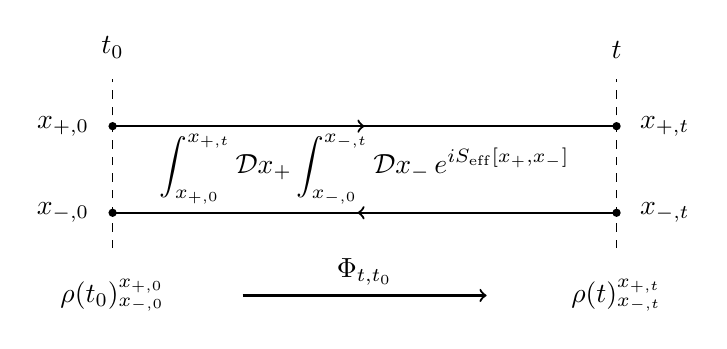
\begin{tikzpicture}[
    x=1cm,
    y=1cm,
    contour/.style={
        thick,
        postaction={decorate}
    },
    forward/.style={
        contour,
        decoration={
            markings,
            mark=at position 0.50 with {\arrow{>}}
        }
    },
    backward/.style={
        contour,
        decoration={
            markings,
            mark=at position 0.50 with {\arrow{<}}
        }
    }
]


\draw[dashed] (0,-1) -- (0,1.15);
\draw[dashed] (6.4,-1) -- (6.4,1.15);


\node[above=4pt] at (0,1.15) {$t_0$};
\node[above=4pt] at (6.4,1.15) {$t$};


\fill (0,0.55) circle (1.5pt);
\fill (0,-0.55) circle (1.5pt);
\fill (6.4,0.55) circle (1.5pt);
\fill (6.4,-0.55) circle (1.5pt);


\draw[forward]  (0,0.55) -- (6.4,0.55);
\draw[backward] (0,-0.55) -- (6.4,-0.55);


\node at (3.2,0)
    {$\displaystyle
    \int_{x_{+,0}}^{x_{+,t}}\mathcal{D}x_+
    \int_{x_{-,0}}^{x_{-,t}}\mathcal{D}x_-\,
    e^{iS_{\mathrm{eff}}[x_+,x_-]}
    $};


\node[left=5pt] at (0,0.55) {$x_{+,0}$};
\node[left=5pt] at (0,-0.55) {$x_{-,0}$};


\node[right=5pt] at (6.4,0.55) {$x_{+,t}$};
\node[right=5pt] at (6.4,-0.55) {$x_{-,t}$};


\node at (0,-1.60)
    {$\rho(t_0)^{x_{+,0}}_{x_{-,0}}$};

\draw[->,thick]
    (1.65,-1.60) -- (4.75,-1.60)
    node[midway,above=0pt]
    {$\displaystyle \Phi_{t,t_0}$};

\node at (6.4,-1.60)
    {$\rho(t)^{x_{+,t}}_{x_{-,t}}$};

\end{tikzpicture}
\caption{閉時間経路を切り開くと、SK経路積分は密度行列を発展させる力学写像$\Phi_{t,t_0}:\rho(t_0)\mapsto\rho(t)$になる。一般の開放系では、二つの枝の時間発展は独立ではなく、影響汎関数によって混合されうることに注意しよう。この正確な意味で、SK経路積分の二つの枝は、密度行列の二つの添字を発展させる。\label{fig:SKdynamicalmap}}
\end{figure}




\paragraph{SK力学写像}



時刻\(t_0\)と\(t_{f}\)の初期・終縮約密度行列は、Kraus表現を用いた\eqref{Krausoperatorrepresentation}のように関係づけられる。本節の記法を使うと、この関係は
\begin{align}\label{rho-kernel}
\rho_S(x_f^+,x_f^-;t_f)
&=
\int dx_i^+\,dx_i^- \;
\mathcal K(t_f,t_0;x_f^+,x_f^-;x_i^+,x_i^-)\,
\rho_S(x_i^+,x_i^-;t_0) ,
\end{align}
となる。ここで\(\mathcal K\)は何らかの核である。\eqref{def:kraus}にあるように、Kraus演算子は時間発展演算子の行列要素なので、経路積分で表せる。したがって、上の核は、切り開いた経路上の経路積分として書ける。
\begin{align}\label{Kkernel}
\mathcal K(t_f,t_0;x_f^+,x_f^-;x_i^+,x_i^-)
&:=
\int_{x_i^+}^{x_f^+}\mathcal D x_+
\int_{x_i^-}^{x_f^-}\mathcal D x_-\;
e^{\,iS_{\rm eff}[x_+,x_-]} .
\end{align}
この記法は、\(+\)と\(-\)の履歴が\(x_i^\pm\)から始まり、\(x_f^\pm\)で終わり、終時刻での接合条件を課さないことを示す。この意味で、閉時間経路を「切り開いた」ことになる。これも引き続き「Schwinger--Keldysh経路積分」と呼ぶが、異なる経路、この場合は分離した経路上で実行される。



式\eqref{rho-kernel}は、Schwinger--Keldysh経路積分が期待値を計算するだけでなく、密度行列上の力学写像を定義するためにも使えることを明らかにする。実際、
\begin{equation}
\rho_S(t_f)=:\Phi_{t_f,t_0}\bigl[\rho_S(t_0)\bigr] ,
\end{equation}
と書くと、核\(\mathcal K\)は単に写像\(\Phi_{t_f,t_0}\)の場の基底での表現である。これを\textit{Schwinger--Keldysh（SK）力学写像}と呼ぶ。図\ref{fig:SKdynamicalmap}にこれを示す。





\paragraph{合成則} 先の節で見たように、陽な時間依存性がある場合、半群性は適用されない。代わりに、力学写像は二つの時刻引数をもち、\eqref{compositionlaw}の合成則を課すべきである。ここでは、有効作用が時間局所的なら、この合成則が直接従うことを証明する。
\begin{equation}\label{localSKaction}
S_{\rm eff}[x_+,x_-]
=
\int_{t_0}^{t_f} dt\,
L
\bigl(
x_+(t),x_-(t),\dot x_+(t),\dot x_-(t),\ldots;t
\bigr) \,,
\end{equation}
が、ある関数$ L$について成り立つとしよう。このとき、\(t_f>t_1>t_0\)を満たす任意の中間時刻\(t_1\)について、作用は加法的に分かれる。
\begin{equation}
S_{\rm eff}^{[t_0,t_f]}[x_+,x_-]
=
S_{\rm eff}^{[t_0,t_1]}[x_+,x_-]
+
S_{\rm eff}^{[t_1,t_f]}[x_+,x_-] .
\end{equation}
したがって、経路積分では、時刻\(t_1\)で恒等演算子の分解を挿入し、中間の境界データ\(\tilde x^\pm:=x_\pm(t_1)\)について積分して、核を連続する二つの部分に因子化できる。その結果、
\begin{align}\label{compositionkernel}
\mathcal K(t_f,t_0;x_f^+,x_f^-;x_i^+,x_i^-)
&=
\int d\tilde x^+\,d\tilde x^- \;
\mathcal K(t_f,t_1;x_f^+,x_f^-;\tilde x^+,\tilde x^-)
\nonumber\\
&\hspace{1.8cm}\times
\mathcal K(t_1,t_0;\tilde x^+,\tilde x^-;x_i^+,x_i^-) .
\end{align}
を得る。よって、演算子の水準では、
\begin{equation}
\Phi_{t_f,t_0}=\Phi_{t_f,t_1}\circ \Phi_{t_1,t_0} .
\end{equation}
となる。したがって、Schwinger--Keldysh有効作用の時間局所性は、力学写像の合成性の十分条件である。



これは半群性よりも弱い条件であることに注意しよう。局所的な有効作用が時間並進不変であるという、さらに特殊な場合にだけ、前節で論じた半群性が再現される。



\paragraph{CP可分性} 時間局所性を仮定すれば、GKSL定理の証明で行ったように、短時間核から時間局所的な生成子を取り出すのが自然である。\(\delta t\)を無限小とする。このとき、区間\([t,t+\delta t]\)の核は
\begin{align}
\mathcal K(t+\delta t,t;x_f^+,x_f^-;x_i^+,x_i^-)
&=
\delta(x_f^+-x_i^+)\,\delta(x_f^--x_i^-)
\nonumber\\
&\qquad
+\,
\delta t\,
\mathcal L_t(x_f^+,x_f^-;x_i^+,x_i^-)
+
\mathcal O(\delta t^2) ,
\end{align}
の形を取る。\(\mathcal L_t\)は時間局所的な生成子の核表示であり、時間依存Liouvillianと呼べる。等価に、写像の微分可能性を仮定すると、
\begin{equation}\label{timelocalgeneratorSK}
\partial_{t_f}\Phi_{t_f,t_0}
=
\mathcal L_{t_f}\circ \Phi_{t_f,t_0} .
\end{equation}
と定義する。すでに見たように、解は超演算子$ \L$の時間順序付き指数関数である。
\begin{equation}
\Phi_{t_f,t_0}
=
T\exp\!\left(
\int_{t_0}^{t_f} ds\,\mathcal L_s
\right) .
\end{equation}
CP可分性を確立するには、この生成子が各時刻\(t\)でGKSL形式であるかを確認する必要がある。写像の微分可能性と可逆性という標準的な仮定のもとで、CP可分性は、
\begin{equation}
\mathcal L_t[\rho]
=
-i[H(t),\rho]
+
\sum_{\alpha,\beta} c_{\alpha\beta}(t)
\left(
L_\alpha(t)\rho L_\beta^\dagger(t)
-\frac12\{L_\beta^\dagger(t)L_\alpha(t),\rho\}
\right) ,
\end{equation}
と書けることと等価である。ここで、あるジャンプ演算子$  L_{\alpha} $に対し、Kossakowski行列\(c_{\alpha\beta}(t)\)はすべての\(t\)で半正定値である。後の小節では、ノイズと散逸を伴う調和振動子を用い、この手順の具体例を示す。





\subsection{例：減衰調和振動子}\label{ssec:dampedharmonic}



Schwinger--Keldysh作用と時間局所的な生成子の関係をより明示するため、単一の量子力学的自由度\(x\)を考えよう。GKSL定理は演算子の位相空間で自然に定式化されるので、正準変数\(x\)と\(p\)の一階作用から直接始めると便利である。質量は議論で本質的な役割を果たさないため、終始1とする。各変数に高々一つの時間微分が作用する、時間局所的なガウス理論に限る。便利な代表例は次である\footnote{運動量変数を積分消去すると、\(x_r\)と\(x_a\)の等価な二階作用を得られる。特に、\(p_r\)についての積分は\(
p_a
=
\dot x_a-\kappa x_a.
\)を課す。その結果、位相空間のノイズ項から\(x_a^2\)、\(\dot x_a^2\)、\(x_a\dot x_a\)に比例する項が生成される。係数が定数なら、最後の項は全微分であり、境界項に置き換えられる。そのため、二階の記述では、情報がバルク係数と境界項または接触項に分散する。したがって、完全正値性の制約は一階形式で最も明瞭であり、本小節の残りではこれを用いる。}。
\begin{align}\label{GaussianSKfirstorder}
S_{\rm SK}[x_r,x_a,p_r,p_a]
=
\int dt \Bigg[
&p_a \dot x_r + p_r \dot x_a
-p_r p_a
-\Omega^2(t)\,x_r x_a
-\kappa(t)\,x_a p_r
\nonumber\\
&\qquad
+\frac{i}{2}N_x(t)\,x_a^2
+\frac{i}{2}N_p(t)\,p_a^2
+iN_{xp}(t)\,x_a p_a
\Bigg].
\end{align}
ここで\(\Omega(t)\)は瞬間的な振動子の周波数、\(\kappa(t)\)は散逸係数であり、\(N_x(t)\)、\(N_p(t)\)、\(N_{xp}(t)\)は、位相空間の対称なノイズ行列の三つの独立成分である。\(N_x\)と\(N_p\)に比例する項は、二つの正準方向のノイズを記述し、\(N_{xp}\)はそれらの交差相関を記述する。





無限小区間\([t,t+\delta t]\)にわたり、核は
\begin{align}\label{dictionary}
\mathcal K(t+\delta t,t)
=
\mathds{1}
+\delta t\,\mathcal L_t
+\mathcal O(\delta t^2),
\end{align}
の形を取る。ここで\(\mathcal L_t\)は時間局所的な生成子である。これをSchwinger--Keldysh核の展開
\begin{equation}
e^{\,iS_{\rm eff}^{[t,t+\delta t]}}
=
1+iS_{\rm eff}^{[t,t+\delta t]}
+\mathcal O(\delta t^2).
\end{equation}
と比較する。\(S_{\rm eff}^{[t,t+\delta t]}\)の一次の項がLiouvillian\(\mathcal L_t\)を決める。得られる表式は、Schwinger--Keldyshの対応関係
\begin{align}
x_a=x_+-x_-
&\longleftrightarrow
[x,\rho],
\\
p_a=p_+-p_-
&\longleftrightarrow
[p,\rho],
\\
x_r=\frac{x_++x_-}{2}
&\longleftrightarrow
\frac{1}{2}\{x,\rho\},
\\
p_r=\frac{p_++p_-}{2}
&\longleftrightarrow
\frac{1}{2}\{p,\rho\}.
\end{align}
を用いて、演算子の言葉に翻訳できる。したがって、先進変数一つは交換子に、遅延変数一つは反交換子に対応する。先進変数と遅延変数の積を扱う場合、経路積分変数を演算子の式に翻訳するには、演算子の順序を指定する必要がある。ここでこれが必要なのは、以下で論じる$ x_{a}p_{r}$という項だけである。その場合、Weyl順序を採用し、対称化した積に上の対応関係を用いる。



特に、先進場について二次の虚の項は、
\begin{align}
\frac{i}{2}N_x(t)\,x_a^2
&\longrightarrow
-\frac{N_x(t)}{2}[x,[x,\rho]],
\\
\frac{i}{2}N_p(t)\,p_a^2
&\longrightarrow
-\frac{N_p(t)}{2}[p,[p,\rho]],
\\
iN_{xp}(t)\,x_a p_a
&\longrightarrow
-\frac{N_{xp}(t)}{2}
[x,[p,\rho]]
=-\frac{N_{xp}(t)}{2}
[p,[x,\rho]]
\end{align}
を与える。ここでは、作用からLiouvillianに移る際の正しい因子$i $を含め、最後の表式をJacobi恒等式と$ [x,p]=i$を使って整理した。これら三つの表式では、演算子順序の指定は不要である。
混合項は、トレースを保存する次のシンボルで表される\footnote{この関係を、$x_a p_r$に対応するシンボルの演算子順序の定義とみなしてもよい。等価に、$x_a$と$p_r$にWeyl順序を課し、\textit{さらに}トレース保存に必要な接触項を含めることで導かれる。}。
\begin{equation}
-\kappa(t)\,x_a p_r
\;\longrightarrow\;
-\frac{i\kappa(t)}{2}[x,\{p,\rho\}] .
\end{equation}
この項を次のように分解すると便利である。
\begin{equation}
-\frac{i\kappa(t)}{2}[x,\{p,\rho\}]
=
-i\left[\frac{\kappa(t)}{4}\{x,p\},\rho\right]
-\frac{i\kappa(t)}{2}\bigl(x\rho p-p\rho x\bigr)
+\frac{\kappa(t)}{2}\rho .
\end{equation}
したがって、マスター方程式は
\begin{align}
\label{GaussianLindbladian}
\frac{d\rho}{dt}
&=
-i[H(t),\rho]
-\frac{i\kappa(t)}{2}\bigl(x\rho p-p\rho x\bigr)
+\frac{\kappa(t)}{2}\rho
\nonumber\\
&\quad
-\frac{N_x(t)}{2}[x,[x,\rho]]
-\frac{N_p(t)}{2}[p,[p,\rho]]
-\frac{N_{xp}(t)}{2}
\Bigl(
[x,[p,\rho]]
+
[p,[x,\rho]]
\Bigr),
\end{align}
と書ける。ここで
\begin{equation}
H(t)
=
\frac{p^2}{2}
+
\frac{1}{2}\Omega^2(t)x^2
+
\frac{\kappa(t)}{4}\{x,p\}.
\end{equation}


である。ここで\eqref{GaussianLindbladian}を、Hamiltonianとすべての係数の時間依存性を許して、\eqref{generalLindbladian}で得た一般的なガウス的GKSL生成子と比較できる。Hermite演算子基底
\begin{equation}
F_1=p,
\qquad
F_2=x,
\end{equation}
では、\eqref{GaussianLindbladian}の散逸部分はKossakowski行列
\begin{equation}
\label{GaussianKossakowski}
C(t)
=
\begin{pmatrix}
N_p(t)
&
N_{xp}(t)+\dfrac{i}{2}\kappa(t)
\\[6pt]
N_{xp}(t)-\dfrac{i}{2}\kappa(t)
&
N_x(t)
\end{pmatrix}.
\end{equation}
によって生成される。実の非対角部分は$N_{xp}$に比例する混合拡散項を生み、虚の反対称部分は摩擦項の非Hamilton的部分
\begin{equation}
-\frac{i\kappa(t)}{2}\bigl(x\rho p-p\rho x\bigr)
+\frac{\kappa(t)}{2}\rho .
\end{equation}
を生む。これを$H(t)$に含めた寄与$\kappa(t)\{x,p\}/4$と合わせると、$-i\kappa(t)[x,\{p,\rho\}]/2$を再構成する。



完全正値性は、
\begin{equation}
C(t)\geq0
\end{equation}
を各時刻で要求する。\(2\times2\)のHermite行列の場合、これは
\begin{equation}
\label{GaussianCPbound}
N_x(t)\geq0,
\qquad
N_p(t)\geq0,
\qquad
N_x(t)N_p(t)-N_{xp}(t)^2
\geq
\frac{\kappa(t)^2}{4}.
\end{equation}
と等価である。これらの不等式は、ガウス的開放系における完全正値性の現れであり、時間局所的な発展で瞬間ごとに成り立つときには、CP可分性の現れでもある。これらは、ゼロでない摩擦係数には、それに伴うノイズの最低量が必要であることを明示する。十分な揺らぎなしに、完全正なMarkov的発展で摩擦が生じることはできない。



この結果を、Schwinger--Keldyshのユニタリ性から直接得られる、より弱い制約と比べると有用である。条件
\begin{equation}
\Im S_{\rm eff}\geq0
\end{equation}
は、実対称なノイズ行列
\begin{equation}
N(t)
=
\begin{pmatrix}
N_p(t) & N_{xp}(t)
\\
N_{xp}(t) & N_x(t)
\end{pmatrix}
\end{equation}
が半正定値であることを要求するため、次だけを導く。
\begin{equation}
N_x(t)\geq0,
\qquad
N_p(t)\geq0,
\qquad
N_x(t)N_p(t)-N_{xp}(t)^2\geq0.
\end{equation}
時間局所的生成子の完全正値性は、散逸係数\(\kappa(t)\)に対するノイズの大きさを制約し、\eqref{GaussianCPbound}の下限を導くため、より強い。二階形式にも同じ制約が存在するが、それは、運動量の積分消去で生成されるバルク項、端点の寄与、接触項の間に分散している。そのため、位相空間における起源は、一階作用で最も明確に見える。





\subsection{ジャンプ演算子と正値性を改善した影響汎関数}



現実的な応用では、環境自由度は通常、第\ref{sec:4p7}節で行ったように厳密に積分消去するには複雑すぎる。したがって、有効場理論（EFT）の考え方を採用し、系の自由度、問題の対称性、適切なべきの数え上げを用いて、SK汎関数をモデル化する必要がある。本小節では、Lindblad方程式でおなじみのジャンプ演算子構造が、時間局所的な影響汎関数を系統的にパラメータ化する方法を与え、完全なSK汎関数の直接的な展開に代えて使えることを説明する。この整理は、完全正値性の制約を明瞭にするだけでなく、打ち切りのもとで厳密な正値性を保つことができ、晩期の再総和のための物理的に許容される出発点を与える。





\paragraph{GKSL方程式から影響汎関数へ。}
次の形の局所的なMarkovマスター方程式を考える。
\begin{equation}
\dot{\rho}
=
-i[H,\rho]
+
C_{\alpha\beta}
\left(
L_{\beta}\rho L_{\alpha}^{\dagger}
-
\frac{1}{2}
\left\{
L_{\alpha}^{\dagger}L_{\beta},
\rho
\right\}
\right),
\end{equation}
繰り返された添字については和を取り、Kossakowski行列は
\begin{equation}\label{Cprop}
C_{\alpha\beta}
=
C_{\beta\alpha}^{*},
\qquad
C\geq 0.
\end{equation}
を満たす。簡単のため、第\ref{ssec:dampedharmonic}節のおもちゃのモデルのように、ジャンプ演算子が経路積分変数の時間局所的な関数$L_{\alpha}(x)$として書き直せるとしよう。
\begin{equation}
L_{\alpha,+}
:=
L_{\alpha}(x_{+}),
\qquad
L_{\alpha,-}
:=
L_{\alpha}(x_{-}),
\end{equation}
と表し、無限小発展の散逸部分に、\eqref{dictionary}の前後で論じた対応関係$ iS_{\rm IF} \sim \int dt \L  $を用いると、Schwinger--Keldysh影響汎関数
\begin{equation}
S_{\mathrm{IF}}
=
-i
\int dt\,
C_{\alpha\beta}
\left[
L_{\alpha,-}^{*}L_{\beta,+}
-
\frac{1}{2}
L_{\alpha,+}^{*}L_{\beta,+}
-
\frac{1}{2}
L_{\alpha,-}^{*}L_{\beta,-}
\right].
\end{equation}
を得る。この表式は、二つの枝が\( S_{\mathrm{IF}}[x,x]
=
0 \)と一致すると自動的にゼロとなり、Schwinger--Keldysh生成汎関数の規格化の要請を満たす。



$ S_{\rm IF}$の実部と虚部への分離をより明示するため、次を定義すると有用である。
\begin{equation}
\Delta L_{\alpha}
:=
L_{\alpha,+}
-
L_{\alpha,-}.
\end{equation}
次の二次形式を展開してみよう。
\begin{align}
\Delta L_{\alpha}^{*}
C_{\alpha\beta}
\Delta L_{\beta}
={}&
L_{\alpha,+}^{*}
C_{\alpha\beta}
L_{\beta,+}
+
L_{\alpha,-}^{*}
C_{\alpha\beta}
L_{\beta,-}-
L_{\alpha,+}^{*}
C_{\alpha\beta}
L_{\beta,-}
-
L_{\alpha,-}^{*}
C_{\alpha\beta}
L_{\beta,+}.
\end{align}
Kossakowski行列はHermiteなので、\(
C_{\alpha\beta}
=
C_{\beta\alpha}^{*},
\)であり、
\begin{equation}
L_{\alpha,+}^{*}
C_{\alpha\beta}
L_{\beta,-}
=
\left(
L_{\alpha,-}^{*}
C_{\alpha\beta}
L_{\beta,+}
\right)^{*}.
\end{equation}
が成り立つ。したがって、
\begin{align}
&
L_{\alpha,-}^{*}
C_{\alpha\beta}
L_{\beta,+}
-
\frac{1}{2}
L_{\alpha,+}^{*}
C_{\alpha\beta}
L_{\beta,+}
-
\frac{1}{2}
L_{\alpha,-}^{*}
C_{\alpha\beta}
L_{\beta,-}
\nonumber\\
&\hspace{1cm}
=
-\frac{1}{2}
\Delta L_{\alpha}^{*}
C_{\alpha\beta}
\Delta L_{\beta}
+
\frac{1}{2}
\left[
L_{\alpha,-}^{*}
C_{\alpha\beta}
L_{\beta,+}
-
\left(
L_{\alpha,-}^{*}
C_{\alpha\beta}
L_{\beta,+}
\right)^{*}
\right]
\nonumber\\
&\hspace{1cm}
=
-\frac{1}{2}
\Delta L_{\alpha}^{*}
C_{\alpha\beta}
\Delta L_{\beta}
+
i\,
\operatorname{Im}
\left(
L_{\alpha,-}^{*}
C_{\alpha\beta}
L_{\beta,+}
\right).
\end{align}
を得る。この恒等式を影響汎関数に代入すると、
\begin{equation}
S_{\mathrm{IF}}
=
\int dt\,
\operatorname{Im}
\left(
L_{\alpha,-}^{*}
C_{\alpha\beta}
L_{\beta,+}
\right)
+
\frac{i}{2}
\int dt\,
\Delta L_{\alpha}^{*}
C_{\alpha\beta}
\Delta L_{\beta}.
\end{equation}
を得る。第一項は明らかに実であり、第二項は\eqref{Cprop}によって純虚数である。さらに、$C\geq0$なので、
\begin{equation}
\operatorname{Im}S_{\mathrm{IF}}
=
\frac{1}{2}
\int dt\,
\Delta L_{\alpha}^{*}
C_{\alpha\beta}
\Delta L_{\beta}
\geq0.
\end{equation}
となる。全体系のユニタリ性が課す\eqref{constraintsra}の最後の制約は、Kossakowski行列の正値性$C\geq0$から直接従うことが分かった。



単一のHermiteなジャンプ演算子、あるいはより一般に、実対称なKossakowski行列を伴うHermiteなジャンプ演算子では、影響汎関数の実部はゼロになることに注意しよう。一般の非Hermiteなジャンプ演算子の場合、またHermiteなジャンプでも、Kossakowski行列の虚の反対称部分をHamiltonianへ吸収する前には、代わりに
\begin{equation}
\operatorname{Re}S_{\mathrm{IF}}
=
\int dt\,
\operatorname{Im}
\left(
L_{\alpha,-}^{*}
C_{\alpha\beta}
L_{\beta,+}
\right).
\end{equation}
となりうる。$ x_{+}=x_{-}$のとき、虚部を取る対象が実数となることに注意しよう。これは必要な性質である。





\paragraph{ジャンプ演算子の展開と影響作用の展開。}
非線形演算子を抑制する短距離の尺度を$d$とし、ジャンプ演算子が$x/d$のべきで展開できるとする。簡単な例として、
\begin{equation}
L_{1}(x)
=
x+\frac{x^{2}}{d},
\qquad
L_{2}(x)
=
\frac{x^{2}}{d},
\end{equation}
を考え、簡単のため、正の率$\gamma_{1}$と$\gamma_{2}$をもつ対角Kossakowski行列を仮定する。対応する影響作用の虚部は
\begin{equation}
\operatorname{Im}S_{\mathrm{IF}}
=
\frac{1}{2}
\int dt\,
\left[
\gamma_{1}\left|\Delta L_{1}\right|^{2}
+
\gamma_{2}\left|\Delta L_{2}\right|^{2}
\right].
\end{equation}
である。理論を$d^{-1}$の次数までだけ構成したいとしよう。自然な処方が二つある。第一は、ジャンプ演算子の展開を打ち切り、$L_{2}$を捨てる一方、$L_{1}$の二次の寄与を完全に残すものである。
\begin{equation}
\operatorname{Im}S_{\mathrm{IF}}^{\mathrm{imp}}
=
\frac{\gamma_{1}}{2}
\int dt\,
\left[
\Delta x
+
\frac{1}{d}\Delta(x^{2})
\right]^{2}.
\end{equation}
この表式を展開すると、
\begin{equation}
\operatorname{Im}S_{\mathrm{IF}}^{\mathrm{imp}}
=
\frac{\gamma_{1}}{2}
\int dt\,
\left[
(\Delta x)^{2}
+
\frac{2}{d}
\Delta x\,\Delta(x^{2})
+
\frac{1}{d^{2}}
\left(\Delta(x^{2})\right)^{2}
\right].
\end{equation}
を得る。最後の項は形式的には$d^{-2}$の次数だが、正の平方を完成させるために保持する。



第二の処方は、影響作用自体を展開し、$d^{-1}$の次数で直接打ち切るものである。このとき、
\begin{equation}
\operatorname{Im}S_{\mathrm{IF}}^{(1/d)}
=
\frac{\gamma_{1}}{2}
\int dt\,
\left[
(\Delta x)^{2}
+
\frac{2}{d}
\Delta x\,\Delta(x^{2})
\right].
\end{equation}
を得る。二つの処方は$d^{-1}$の次数まで一致し、$d^{-2}$の次数でのみ異なる。どちらの表式も$ d^{-2}$の次数の完全な答えではない。$L_{2}$のような追加のジャンプ演算子や、対称性が許す他の項も寄与しうるからである。



それでも、第一の処方には構造的な利点がある。打ち切ったジャンプ演算子に対応する完全な平方を保持することで、任意の場の配置に対して\(
\operatorname{Im}S_{\mathrm{IF}}^{\mathrm{imp}}
\geq0
\)を保証する。等価に、対応する打ち切られたLiouvillianはGKSL形式を保ち、完全正かつCP可分な発展を生成する。対照的に、$d^{-1}$の次数で直接打ち切った影響作用は、任意の$x_{+}$と$x_{-}$について符号が確定しない。その正値性は、$x/d$が小さい領域で、摂動的にしか意味をもたない。



第一の処方を、\emph{正値性を改善した}打ち切りと呼んでもよい。これは$d^{-2}$の次数での完全な答えを決めるものではないが、完全正値性を厳密に保存する特定の高次の補完を与える。この違いは、厳密に固定次数で計算する場合には重要でないが、第\ref{ssec:resummation}節のように打ち切った生成子を時間について非摂動的に発展させる場合には有用になりうる。得られる再総和が完全正のまま保たれるためである。この状況は、固定次数のループ計算の一部を繰り込み群で改善する際に起こることと、構造的に似ている。






\subsection{半古典極限、HS変換、Langevin動力学}





\(r/a\)基底で書いた一般の局所的Schwinger--Keldysh作用$ S_{\rm eff}[x_r,x_a]   $から始めよう。次が成り立つことに注意する。
\begin{align}
\langle \! \langle x_{r} \rangle \! \rangle &= \frac{1}{2} (\langle \! \langle x_{+} \rangle \! \rangle+\langle \! \langle x_{-} \rangle \! \rangle)=\ex{x}\,, & \langle \! \langle x_{a} \rangle \! \rangle  &= \langle \! \langle x_{+} \rangle \! \rangle-\langle \! \langle x_{-} \rangle \! \rangle=0 \,.
\end{align}
これは、$ x_{r} $が演算子$ x $の平均的な古典部分を捉え、$ x_{a}$が経路積分で古典的鞍点から外れる揺らぎを捉えることを示唆する。その揺らぎは量子的起源でも確率的起源でもありうる。



より具体的にするため、規格化条件\(S_{\rm eff}[x_r,0]=0\)により、作用が少なくとも一つの\(x_a\)の因子を含むことにも注目する。\(x_a\)が小さい領域では、作用を
\begin{align}\label{aeexpansion}
S_{\rm eff}[x_r,x_a]
&=
\int dt\, x_a(t)\,\mathcal E[x_r](t)
+\frac{i}{2}\int dt\,dt'\,x_a(t)\,N(t,t')\,x_a(t') +\mathcal O(x_a^3) .
\end{align}
と展開するのが自然である。ここで\(\mathcal E[x_r](t)\)は遅延場の何らかの汎関数、\(N(t,t')\)は実対称な核である。\(x_a\)の一次項は、先進場について変分してから\(x_a=0\)と置いたときに残る部分である。二次項は、Schwinger--Keldyshの正値性条件が許す最低次の虚の寄与である。\(x_a\)の高次のべきは、有効動力学への本質的に量子的な、あるいは非ガウス的な補正を符号化する。



半古典的な確率極限は、\eqref{aeexpansion}を\(x_a\)の二次で打ち切ることで得られる。
\begin{equation}\label{quadratictruncate}
S_{\rm eff}[x_r,x_a]
\approx
\int dt\, x_a(t)\,\mathcal E[x_r](t)
+\frac{i}{2}\int dt\,dt'\,x_a(t)\,N(t,t')\,x_a(t') .
\end{equation}
この段階でHubbard--Stratonovich変換が有用となる。核\(N(t,t')\)は半正定値なので、ガウス恒等式
\begin{align}\label{HSidentity}
\exp\!\left[
-\frac12\int dt\,dt'\,x_a(t)\,N(t,t')\,x_a(t')
\right]
&\propto
\int \mathcal D\xi\;
\exp\Biggl[
-\frac12\int dt\,dt'\,\xi(t)\,N^{-1}(t,t')\,\xi(t')
\nonumber\\
&\hspace{2.4cm}
+i\int dt\,\xi(t)\,x_a(t)
\Biggr] .
\end{align}
を用いられる。ここで\(\xi(t)\)は補助場である。作用を\(x_a\)の二次で打ち切っている限り、変換\eqref{HSidentity}は厳密である。これを経路積分に挿入すると、有効作用は先進場について線形になり、
\begin{equation}
S_{\rm eff}[x_r,x_a,\xi]
=
\int dt\,x_a(t)\bigl(\mathcal E[x_r](t)-\xi(t)\bigr) ,
\end{equation}
となる。ただし、\(\xi\)に対するガウスの重みは別に残る。このとき\(x_a\)の経路積分は厳密に実行でき、汎関数Diracデルタを生み、
\begin{equation}\label{LangevinGeneral}
\mathcal E[x_r](t)=\xi(t) .
\end{equation}
を課す。これが、打ち切ったSchwinger--Keldysh作用に対応するLangevin型の確率方程式である。



補助場\(\xi\)は平均ゼロ、二点関数
\begin{equation}
\langle \xi(t)\xi(t')\rangle_\xi = N(t,t') ,
\end{equation}
のガウス分布に従う。平均は\eqref{HSidentity}に現れるガウス測度について取る。したがって、核\(N(t,t')\)が確率過程のノイズ相関関数となる。このように、先進場の二次項はガウスノイズとして再解釈され、\(x_a\)の一次項は決定論的なドリフト、あるいは運動方程式となる。



この論理は、先に論じたガウス型の例で説明できる。局所的な有効作用が
\begin{equation}
S_{\rm eff}[x_r,x_a]
=
\int dt\,
\left[
x_a\bigl(\ddot x_r+\kappa \dot x_r+\Omega^2 x_r\bigr)
+\frac{i}{2}N\,x_a^2
\right] ,
\end{equation}
の形を取るとしよう。簡単のため、局所的な白色ノイズ核\(N(t,t')=N\,\delta(t-t')\)を書いた。Hubbard--Stratonovich変換は、相関関数
をもつガウス場\(\xi(t)\)を導入する。
\begin{equation}
\langle \xi(t)\xi(t')\rangle_\xi = N\,\delta(t-t') ,
\end{equation}
そして、\(x_a\)についての経路積分は
\begin{equation}
\ddot x_r+\kappa \dot x_r+\Omega^2 x_r=\xi(t) .
\end{equation}
を与える。これは、ガウス白色ノイズで駆動される減衰調和振動子の通常の\textit{Langevin方程式}である。したがって、Schwinger--Keldysh記述は、有効作用を先進場の二次で打ち切ると、なじみ深い確率的記述を再現する。



この構成で何が厳密で、何が近似なのかを把握しておくことが重要である。Hubbard--Stratonovich変換は二次形式についての厳密な恒等式である。近似なのは、Schwinger--Keldysh作用を\(x_a\)について高々二次に打ち切ることである。\(x_a\)の高次のべきがあるなら、単純なガウスノイズ表現はもはや厳密ではない。そうした項は、通常のLangevin動力学を超える非ガウス揺らぎ、あるいは本質的な量子補正に対応する。





\paragraph{Langevin方程式からFokker--Planck方程式へ} ノイズ$ \xi(t)$の各実現に対し、Langevin方程式は$ x(t)$の時間発展の一つの実現を与える。ノイズの実現の分布から、ある時刻$ t$で$ x$が取る値の確率分布$ P(x,t)$が得られる。ここでは、$ P(x,t)$が満たす微分方程式を導く。簡単のため、以下で指定する加法的なガウス白色ノイズを伴う、一階のLangevin方程式に限定する。この制限により、乗法的ノイズで重要になるIt\^o処方とStratonovich処方の区別を避けられる。高階時間微分を含むLangevin方程式は、例えば位置と速度を独立変数として扱うなど、力学変数の空間を拡大することで一階形式にできる。



確率方程式
\begin{equation}
\dot{x}(t)
=
A\bigl(x(t)\bigr)
+
\xi(t),
\label{firstorderlangevin}
\end{equation}
を考える。ここで\(A(x)\)は決定論的ドリフト、\(\xi(t)\)は次を満たすガウス白色ノイズである。
\begin{equation}
\langle \xi(t) \rangle_{\xi}
=
0,
\qquad
\langle \xi(t)\xi(t') \rangle_{\xi}
=
N\,\delta(t-t').
\label{additivewhitenoise}
\end{equation}
Langevin方程式は個々の確率的軌道を記述する。ここでの目標は、それに代えて、確率変数が時刻\(t\)に値\(x\)を取る確率密度\(P(x,t)\)を決定することである。



短い区間\(\Delta t\)では、式\eqref{firstorderlangevin}は
\begin{equation}
\Delta x
=
A(x)\Delta t
+
\Delta W,
\label{shorttimeincrement}
\end{equation}
を与える。ここで
\begin{equation}
\Delta W
\equiv
\int_{t}^{t+\Delta t}dt'\,\xi(t')
\end{equation}
は、次を満たすガウス確率変数である。
\begin{equation}
\langle \Delta W\rangle_{\xi}
=
0,
\qquad
\langle (\Delta W)^{2}\rangle_{\xi}
=
N\Delta t.
\end{equation}
このことから、
\begin{align}
\langle \Delta x\rangle_{\xi}
&=
A(x)\Delta t,
\\
\langle (\Delta x)^{2}\rangle_{\xi}
&=
N\Delta t
+
\mathcal O\bigl((\Delta t)^{2}\bigr).
\end{align}
が従う。\(\Delta x\)の高次モーメントは\(\Delta t\)より高次であり、連続極限では寄与しない。



\(f(x)\)を任意の滑らかな試験関数とする。短い区間\(\Delta t\)の間に、
\begin{equation}
f(x+\Delta x)
=
f(x)
+
f'(x)\Delta x
+
\frac{1}{2}f''(x)(\Delta x)^{2}
+
\cdots .
\end{equation}
となる。ノイズについて平均し、\(\Delta t\)の次数の項を残すと、
\begin{equation}
\left\langle
f(x+\Delta x)-f(x)
\right\rangle_{\xi}
=
\left[
A(x)f'(x)
+
\frac{N}{2}f''(x)
\right]
\Delta t
+
\mathcal O\bigl((\Delta t)^{2}\bigr).
\end{equation}
を得る。連続極限を取ると、
\begin{equation}
\frac{d}{dt}
\left\langle
f(x)
\right\rangle
=
\left\langle
A(x)f'(x)
+
\frac{N}{2}f''(x)
\right\rangle.
\label{testfunctionevolution}
\end{equation}


となる。\(f\)の期待値は、確率密度を用いても次のように書ける。
\begin{equation}
\left\langle
f(x)
\right\rangle
=
\int dx\,P(x,t)f(x).
\end{equation}
したがって、
\begin{equation}
\frac{d}{dt}
\left\langle
f(x)
\right\rangle
=
\int dx\,
f(x)
\frac{\partial P(x,t)}{\partial t}.
\label{expectationfromP}
\end{equation}
である。一方、\eqref{testfunctionevolution}を用いると、
\begin{equation}
\frac{d}{dt}
\left\langle
f(x)
\right\rangle
=
\int dx\,P(x,t)
\left[
A(x)f'(x)
+
\frac{N}{2}f''(x)
\right].
\end{equation}
となる。部分積分を行い、境界項が消えると仮定すれば、
\begin{equation}
\frac{d}{dt}
\left\langle
f(x)
\right\rangle
=
\int dx\,f(x)
\left[
-
\frac{\partial}{\partial x}
\left(
A(x)P(x,t)
\right)
+
\frac{N}{2}
\frac{\partial^{2}P(x,t)}{\partial x^{2}}
\right].
\end{equation}
を得る。\(f(x)\)は任意なので、\eqref{expectationfromP}と比べることにより、\textit{Fokker--Planck方程式}
\begin{equation}
\frac{\partial P(x,t)}{\partial t}
=
-
\frac{\partial}{\partial x}
\left[
A(x)P(x,t)
\right]
+
\frac{N}{2}
\frac{\partial^{2}P(x,t)}{\partial x^{2}}.
\label{fokkerplanckgeneral}
\end{equation}


を得る。第一項は、決定論的ドリフト\(A(x)\)に従って確率を輸送し、第二項は確率的ノイズによる拡散を記述する。この結果は、第\ref{sec:stochastic}節でde Sitter時空の軽いスカラー場を記述するために用いる。



\eqref{fokkerplanckgeneral}を連続の方程式
\begin{equation}
\frac{\partial P}{\partial t}
=
-
\frac{\partial J}{\partial x},
\end{equation}
として書くと有用な場合が多い。ここで確率流は
\begin{equation}
J(x,t)
=
A(x)P(x,t)
-
\frac{N}{2}
\frac{\partial P(x,t)}{\partial x}.
\end{equation}


である。完全を期して、一階Langevin方程式の系
\begin{equation}
\dot{X}^{I}
=
A^{I}(X)
+
\xi^{I}(t),
\end{equation}
を、加法的ガウスノイズ
\begin{equation}
\left\langle
\xi^{I}(t)\xi^{J}(t')
\right\rangle_{\xi}
=
N^{IJ}\delta(t-t').
\end{equation}
とともに考える。対応する確率密度\(P(X,t)\)は
\begin{equation}
\frac{\partial P}{\partial t}
=
-
\frac{\partial}{\partial X^{I}}
\left[
A^{I}(X)P
\right]
+
\frac{1}{2}
N^{IJ}
\frac{\partial^{2}P}
{\partial X^{I}\partial X^{J}}.
\end{equation}
に従う。高階のLangevin方程式も、動力学がこのような一階の系で書けるまで変数を追加すれば、扱うことができる。





\paragraph{Martin--Siggia--Roseの構成}



SK経路積分の半古典極限との関係をよりよく理解するため、一般の確率的常微分方程式に対するMartin--Siggia--Roseの構成\cite{PhysRevA.8.423}を簡単に振り返ると有用である。\(I=1,\dots,N_r\)として、次に従う実変数の集合\(\phi^I(t)\)を考える。
\begin{equation}
E^i[\phi](t)=\xi^i(t) ,
\end{equation}
ここで、\(i=1,\dots,N_a\)に対する\(E^i[\phi]\)は、非線形でもよい何らかの微分演算子であり、\(\xi^i(t)\)は確率的ノイズである。具体的に、ノイズは平均ゼロ、共分散
\begin{equation}
\langle \xi^i(t)\,\xi^j(t')\rangle
=
N^{ij}(t,t') .
\end{equation}
のガウスノイズとする。関心があるのは、ノイズの実現について平均した、場\(\phi^I\)の統計的性質を予言することである。この設定に量子力学はない。これは古典的な確率問題である。



Martin、Siggia、Roseの中心的な考えは、この確率平均を汎関数積分として書き直すことである。まず、ノイズ平均に、確率方程式を課す汎関数デルタを挿入する\footnote{簡単のため、この導出では$  N_{r}=N_{a} $と仮定し、Jacobianが単なる行列式となるようにする。ただし、MSR形式は$  N_{a}\neq N_{r} $にも一般化できる。}。
\begin{equation}
1=
\int \mathcal D\phi\;
\delta\!\bigl(E[\phi]-\xi\bigr)\,
\det\!\left(\frac{\delta E}{\delta \phi}\right) ,
\end{equation}
ここで行列式は、\(\phi\)から\(E[\phi]\)への変数変換に伴うJacobianである。次に、しばしば応答場と呼ばれる補助場\(\hat\phi_i(t)\)を導入し、デルタ汎関数を指数関数で表せる。
\begin{equation}
\delta\!\bigl(E[\phi]-\xi\bigr)
\propto
\int \mathcal D\hat\phi\;
\exp\!\left[
i\int dt\,\hat\phi_i(t)\bigl(E^i[\phi](t)-\xi^i(t)\bigr)
\right] .
\end{equation}
この段階で、経路積分は依然として厳密である。



ノイズがガウス的なら、\(\xi\)についての平均を具体的に実行できる。これにより応答場の二次の項が生じ、Martin--Siggia--Rose作用
\begin{align}
S_{\rm MSR}[\phi,\hat\phi]
&=
\int dt\,\hat\phi_i(t)\,E^i[\phi](t)
+\frac{i}{2}\int dt\,dt'\,
\hat\phi_i(t)\,N^{ij}(t,t')\,\hat\phi_j(t')
\nonumber\\
&\qquad
+S_{\rm Jac}[\phi,\hat\phi] .
\end{align}
を得る。\(S_{\rm Jac}\)はJacobianの寄与を表し、多くの簡単な場合には規格化に吸収でき、必要ならゴーストで表せる。得られた汎関数積分は、元のLangevin系の確率的相関関数を生成する。\(\hat\phi_i\)の一次項は運動方程式の決定論的部分を課し、二次項はノイズの統計を符号化する。この意味で、応答場はノイズ平均によって修飾されたLagrange未定乗数である。



この構成は、最も単純なLangevin方程式より一般的である。非線形微分方程式、離散化に適切に注意した乗法的ノイズ、非局所核\(N^{ij}(t,t')\)にも適用できる。要点は常に同じである。確率的動力学は、元の変数と、各方程式に一つずつの補助応答場についての経路積分で表され、ノイズ平均が応答場の二次項を、非ガウスノイズではさらに高次の項を生成する。



Schwinger--Keldysh形式の半古典極限との関係を強調しておく。その文脈では、有効作用を先進場のべきで展開する。それらの場の一次と二次の項で作用を打ち切ると、Martin--Siggia--Rose作用と全く同じ構造が得られる。一次項は有効的な運動方程式を課し、二次項はHubbard--Stratonovich変換の後にガウスノイズと解釈できる。この意味で、Martin--Siggia--Rose形式は、Schwinger--Keldysh経路積分に対応する確率的な半古典形式とみなせる。





\subsection{散逸するガウス的スカラー場とその伝播子}



ここからは、単一の変数$ x(t)$から場$\phi(t,\mathbf x) $へ移ると便利である。背景が一様・等方なら、空間についてFourier変換するのが自然である。
\begin{equation}
\phi(t,\mathbf x)
=
\int \frac{d^d k}{(2\pi)^d}\,
e^{i\mathbf k\cdot \mathbf x}\,\phi_{\mathbf k}(t) .
\end{equation}
すると二次の理論では異なる運動量が分離し、各Fourierモード\(\phi_{\mathbf k}(t)\)は、前の小節までで論じた単一変数に対応するように振る舞う。この意味で、自由な、あるいはガウス的な場の理論は、\(\mathbf k\)をラベルとする、互いに結合しない振動子の集合とみなせる。もちろん、場の量子論には量子力学に加えてさらなる複雑さがあり、ループ発散や繰り込みなどのいくつかには、必要な場面で触れることにする。



それに応じて、Schwinger--Keldyshの二重化した変数は\(\phi_\pm(t,\mathbf x)\)、あるいは等価に、
\begin{equation}
\phi_r(t,\mathbf x):=\frac{\phi_+(t,\mathbf x)+\phi_-(t,\mathbf x)}{2},
\qquad
\phi_a(t,\mathbf x):=\phi_+(t,\mathbf x)-\phi_-(t,\mathbf x) .
\end{equation}
となる。ここではMinkowski時空の最も簡単な散逸ガウス模型を考える。\(r/a\)基底での二次Schwinger--Keldysh作用を
\begin{align}\label{DissipativeFieldAction}
S_{\rm SK}
=
\int dt\,\frac{d^d k}{(2\pi)^d}\,
\Bigg[
&\phi_a(-\mathbf k,t)
\Bigl(
\partial_t^2+\gamma\,\partial_t+\omega_{\mathbf k}^2
\Bigr)\phi_r(\mathbf k,t)
\nonumber\\
&\qquad
+\frac{i}{2}\,\mathcal N_{\mathbf k}\,
\phi_a(-\mathbf k,t)\phi_a(\mathbf k,t)
\Bigg] ,
\end{align}
とする。ここで
\begin{equation}
\omega_{\mathbf k}^2:=\mathbf k^2+m^2 .
\end{equation}
である。\(\gamma\)は減衰係数、\(\mathcal N_{\mathbf k}\geq 0\)はKeldysh核、あるいはノイズ核である。ユニタリな全体系から受け継がれる制約、特に
\[ -S_{\rm SK}[\phi_{r},-\phi_{a}]^{*}=S_{\rm SK}[\phi_{r},\phi_{a}]\,, \]
により、$ \gamma $と$ \mathcal{N}$はともに実数でなければならない。
この作用は時間局所的で、二次であり、空間と時間の並進に対して不変である。したがって、すべての伝播子を具体的に計算できる、特に簡単な検討の場となる。



周波数空間で、
\begin{equation}
\phi(\omega,\mathbf k)
=
\int dt\,e^{i\omega t}\phi(t,\mathbf k) ,
\end{equation}
とすると、作用は
\begin{align}
S_{\rm SK}
=
\int \frac{d\omega}{2\pi}\frac{d^d k}{(2\pi)^d}
\Bigg[
\phi_a(-\omega,-\mathbf k)\,
\mathcal D_R(\omega,\mathbf k)\,
\phi_r(\omega,\mathbf k)
+\frac{i}{2}\mathcal N_{\mathbf k}\,
\phi_a(-\omega,-\mathbf k)\phi_a(\omega,\mathbf k)
\Bigg] ,
\end{align}
となる。遅延逆核は
\begin{equation}\label{DRkernel}
\mathcal D_R(\omega,\mathbf k)
=
-\omega^2-i\gamma\omega+\omega_{\mathbf k}^2 .
\end{equation}
であり、先進核はその共役である。
\begin{equation}
\mathcal D_A(\omega,\mathbf k)
=
-\omega^2+i\gamma\omega+\omega_{\mathbf k}^2
=
\mathcal D_R(\omega,\mathbf k)^* .
\end{equation}


理論がガウス的なので、伝播子は二次核の逆を取ることで得られる。計算の詳細は付録\ref{appA}に示す。\(r/a\)基底では、次を得る\footnote{閉じた場の量子論の自由場伝播子との違いに注意しよう。そこでは、逆二次演算子は通常、質量殻上でゼロになるため、逆を取るには、よく知られた\(i\epsilon\)のような追加の処方が必要となる。対照的に、ここでは遅延逆核はすでに\(\gamma  \)に比例する有限の虚部を含むため、実の運動学的変数に対して分母はゼロにならず、極は自動的に実軸を離れ、下半平面へ移る。したがって、逆を取る操作に曖昧さはない。}。
\begin{align}
G_R(\omega,\mathbf k)
&=
\langle\!\langle \phi_r(\omega,\mathbf k)\phi_a(-\omega,-\mathbf k)\rangle\!\rangle
=
\frac{1}{\mathcal D_R(\omega,\mathbf k)}
=
\frac{1}{-\omega^2-i\gamma\omega+\omega_{\mathbf k}^2} ,
\label{GRfreq}
\\
G_A(\omega,\mathbf k)
&=
\langle\!\langle \phi_a(\omega,\mathbf k)\phi_r(-\omega,-\mathbf k)\rangle\!\rangle
=
\frac{1}{\mathcal D_A(\omega,\mathbf k)}
=
\frac{1}{-\omega^2+i\gamma\omega+\omega_{\mathbf k}^2} ,
\label{GAfreq}
\\
G_K(\omega,\mathbf k)
&=
\langle\!\langle \phi_r(\omega,\mathbf k)\phi_r(-\omega,-\mathbf k)\rangle\!\rangle
=
-\,i\,\mathcal N_{\mathbf k}\,
G_R(\omega,\mathbf k)\,G_A(\omega,\mathbf k)
\nonumber\\
&=
-\,i\,\mathcal N_{\mathbf k}\,
\frac{1}{\bigl(-\omega^2-i\gamma\omega+\omega_{\mathbf k}^2\bigr)
\bigl(-\omega^2+i\gamma\omega+\omega_{\mathbf k}^2\bigr)} ,
\label{GKfreq}
\\
G_{aa}(\omega,\mathbf k)
&=
\langle\!\langle \phi_a(\omega,\mathbf k)\phi_a(-\omega,-\mathbf k)\rangle\!\rangle
=
0 .
\end{align}
このように、遅延伝播子と先進伝播子は、$ \phi_{a}$に関して線形な作用の決定論的部分だけで決まる。一方、Keldysh伝播子はノイズ核\(\mathcal N_{\mathbf k}\)にも依存する。



これらの伝播子を\(\pm\)基底で書き直すと有用である。
\begin{align}
G_{++}
&:=
\langle\!\langle \phi_+\phi_+\rangle\!\rangle
=
G_K+\frac12 G_R+\frac12 G_A ,
\\
G_{--}
&:=
\langle\!\langle \phi_-\phi_-\rangle\!\rangle
=
G_K-\frac12 G_R-\frac12 G_A ,
\\
G_{+-}
&:=
\langle\!\langle \phi_+\phi_-\rangle\!\rangle
=
G_K-\frac12 G_R+\frac12 G_A ,
\\
G_{-+}
&:=
\langle\!\langle \phi_-\phi_+\rangle\!\rangle
=
G_K+\frac12 G_R-\frac12 G_A .
\end{align}
言い換えると、\(G_R\)、\(G_A\)、\(G_K\)が分かれば、\(\pm\)基底のすべての経路順序付き伝播子が決まる。



時間領域の遅延伝播子を論じよう。定義より、これは次の遅延Green関数である。
\begin{equation}
\Bigl(\partial_t^2+\gamma\partial_t+\omega_{\mathbf k}^2\Bigr)G_R(t,\mathbf k)
=
\delta(t) ,
\qquad
G_R(t,\mathbf k)=0 \quad \text{ただし } t<0 .
\end{equation}
Fourier変換で時間領域へ戻すと、



\footnote{有限の物理的減衰係数$\gamma>0$では、$G_R$の極は複素$\omega$平面の下半分へ移り、質量ゼロのゼロモードを除き、実周波数の積分経路上には存在しない。したがって、このFourier変換に追加の$i\epsilon$処方は必要ない。$\gamma=0$の場合には極が実軸へ戻るため、通常の遅延処方
\begin{equation}
\mathcal D_R(\omega,\mathbf k)
=
-\omega^2+\mathbf k^2+m^2-i\epsilon\omega,
\qquad
\epsilon\to0^+.
\end{equation}
によってFourier変換を定義しなければならない。したがって、遅延の$i\epsilon$処方は、無限小の正の減衰係数の導入とみなせる。}



（詳細は付録\ref{appA}参照）、不足減衰領域$ \gamma \leq 2\omega_{k}$では、
\begin{equation}\label{GRtime}
G_R(t,\mathbf k)
=
\theta(t)\,
e^{-\gamma t/2}
\frac{\sin(\Omega_{\mathbf k}t)}{\Omega_{\mathbf k}},
\qquad
\Omega_{\mathbf k}
:=
\sqrt{\mathbf k^2+m^2-\frac{\gamma^2}{4}}.
\end{equation}
を得る。また、過減衰領域$ \gamma \geq 2\omega_{k}$では、
\begin{equation}
G_R(t,\mathbf k)
=
\theta(t)\,
\frac{
e^{-(\gamma/2-\Lambda_{\mathbf k})t}
-
e^{-(\gamma/2+\Lambda_{\mathbf k})t}
}{
2\Lambda_{\mathbf k}
}, \qquad  \Lambda_{\mathbf k}
:=
\sqrt{\frac{\gamma^2}{4}-\mathbf k^2-m^2}.
\end{equation}
となる。したがって、$\mathbf k^2+m^2>0$を満たすすべてのモードでは、過去の記憶は指数関数的に抑制されたものしか残らない。不足減衰領域では、包絡線は時間尺度$2/\gamma$で減衰する。一方、過減衰領域では、晩期の減衰はモード依存の率
\begin{equation}
\Gamma_{\rm slow}
=
\frac{\gamma}{2}-\Lambda_{\mathbf k}
\simeq
\frac{\mathbf k^2+m^2}{\gamma},
\end{equation}
によって制御される。最後の表式は$\mathbf k^2+m^2\ll\gamma^2$で成り立つ。したがって、対応する記憶時間は$\mathbf k^2+m^2\to0$で任意に長くなる。厳密に質量ゼロの一様モード$ m=k=0$では、
\begin{equation}
G_R(t,\mathbf 0)
=
\theta(t)\,
\frac{1-e^{-\gamma t}}{\gamma},
\end{equation}
となり、晩期に減衰するのではなく、定数へ近づく。






\begin{figure}
\centering
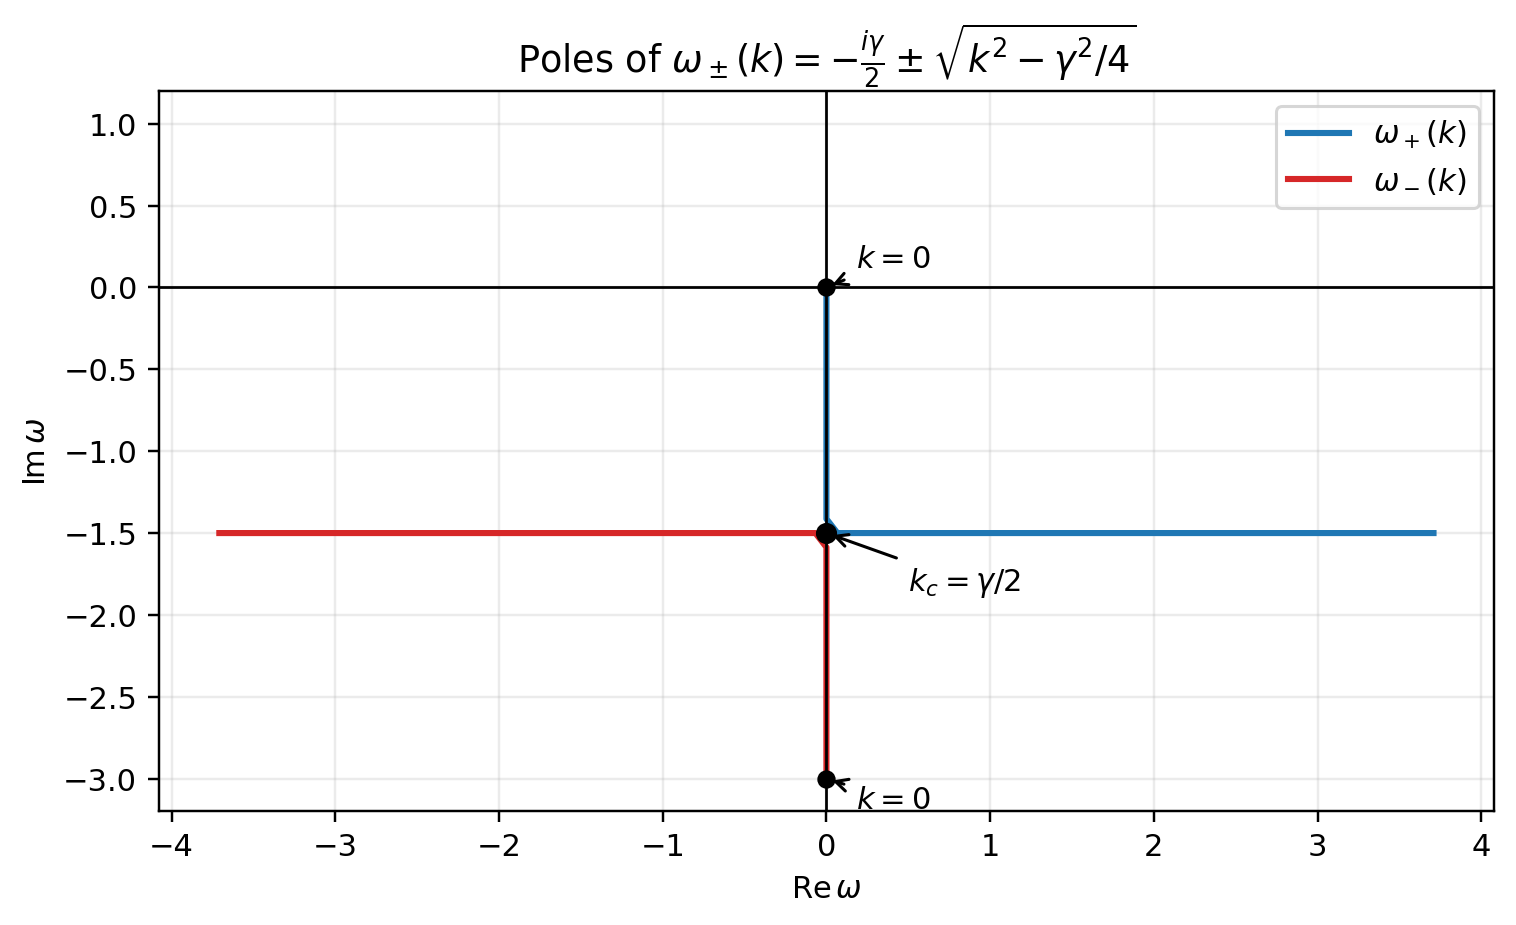
\includegraphics[width=0.9\textwidth]{figures/dispersion.png}
\caption{質量ゼロの散逸モードについて、複素周波数平面における遅延伝播子の極を示す。\(k<\gamma/2\)では両方の極が負の虚軸上にある。\(k=\gamma/2\)で合流し、\(k>\gamma/2\)では虚部\(-\gamma/2\)を一定に保って水平方向へ移動する。\label{dispersion}}
\end{figure}



\paragraph{分散関係} 関心のある分散関係を定義する遅延伝播子の極は、\(\mathcal D_R(\omega,\mathbf k)\)のゼロ点で与えられる。
\begin{equation}
-\omega^2-i\gamma\omega+\omega_{\mathbf k}^2=0 .
\end{equation}
したがって、それらは
\begin{equation}\label{poles}
\omega_\pm(\mathbf k)
=
-\frac{i\gamma}{2}
\pm
\sqrt{\omega_{\mathbf k}^2-\frac{\gamma^2}{4}} .
\end{equation}
である。これらの極は、遅延伝播子に要求されるとおり、常に複素\(\omega\)平面の下半分にある。質量ゼロの場合を図\ref{dispersion}に示す。それらの具体的な形によって、異なる領域が区別される。



不足減衰領域、
\begin{equation}
\gamma<2\omega_{\mathbf k},
\end{equation}
では、\eqref{poles}の平方根は実で、極はゼロでない実部をもつ。対応するモードは周波数\(\Omega_{\mathbf k}\)で振動しつつ、率\(\gamma/2\)で減衰する。



臨界減衰、
\begin{equation}
\gamma=2\omega_{\mathbf k},
\end{equation}
では、二つの極が一致する。
\begin{equation}
\omega_+(\mathbf k)=\omega_-(\mathbf k)=-i\gamma/2 .
\end{equation}


過減衰領域、
\begin{equation}
\gamma>2\omega_{\mathbf k},
\end{equation}
では、平方根は純虚数となり、両方の極が純虚数となる。
\begin{equation}
\omega_\pm(\mathbf k)
=
-\frac{i\gamma}{2}
\pm
i\sqrt{\frac{\gamma^2}{4}-\omega_{\mathbf k}^2} .
\end{equation}
この場合、二つのモードはもはや振動せず、純粋に緩和する。低運動量極限で$  m=0 $の場合には、低周波の「拡散的」モード
\begin{equation}
\omega(\mathbf k)\sim -\,iD\,\mathbf k^2+\cdots .
\end{equation}


が得られる。遅延伝播子の実部と虚部にも触れておくと有用である。
\begin{equation}
G_R(\omega,\mathbf k)
=
\frac{\omega_{\mathbf k}^2-\omega^2+i\gamma\omega}
{\bigl(\omega_{\mathbf k}^2-\omega^2\bigr)^2+\gamma^2\omega^2} ,
\end{equation}
と書けば、
\begin{align}
\Re G_R(\omega,\mathbf k)
&=
\frac{\omega_{\mathbf k}^2-\omega^2}
{\bigl(\omega_{\mathbf k}^2-\omega^2\bigr)^2+\gamma^2\omega^2} ,
\\
\Im G_R(\omega,\mathbf k)
&=
\frac{\gamma\omega}
{\bigl(\omega_{\mathbf k}^2-\omega^2\bigr)^2+\gamma^2\omega^2} .
\end{align}
を得る。実部は分散的で共鳴の近くで符号を変え、虚部は\(\omega\)について奇関数であり、散逸による幅の広がりを測る。特に、極の有限幅は\(\gamma\)によって制御される。



最後に、Keldysh伝播子は具体的に
\begin{equation}
G_K(\omega,\mathbf k)
=
-\,i\,\mathcal N_{\mathbf k}\,
\frac{1}
{\bigl(\omega_{\mathbf k}^2-\omega^2\bigr)^2+\gamma^2\omega^2} .
\end{equation}
となる。これは周波数について偶関数であり、その振幅はノイズ核に直接比例する。



この段階では\(\mathcal N_{\mathbf k}\)は任意である。さらに熱平衡を仮定する場合にだけ、揺動散逸関係あるいはKMS関係によって、遅延・先進伝播子と関係づけられる。この点は後で論じる。



まとめると、散逸するガウス的スカラー場は、すべてのSchwinger--Keldysh伝播子を具体的に計算できる、簡単ながら示唆的な例である。遅延・先進伝播子は逆核\(\mathcal D_R\)と\(\mathcal D_A\)によって決まり、Keldysh伝播子はノイズスペクトルを符号化する。\(\pm\)基底の経路順序付き伝播子は、これらから再構成される。遅延極の位置は、励起が不足減衰、臨界減衰、過減衰のどれであるかを示す。一方、真に拡散的なモードは、さらに低周波・低運動量の極限を取った場合にだけ現れる。





\section{宇宙論とインフレーション}\label{sec:5}



ここから、本ノートの残りの主な舞台となる宇宙論的設定へ進む。最終的な目標は、開放量子系、マスター方程式、Schwinger--Keldysh有効作用の道具を、原始宇宙、特にインフレーションにどう適用できるかを理解することである。ただし、その前に、対応する閉鎖系の記述を振り返ると有用である。インフレーションは、場の量子論にとって注目すべき検討の場となる。背景時空は時間に依存し、関心のある観測量は散乱振幅ではなく晩期の相関関数であり、初期宇宙で生成された揺らぎが、今日空に観測される構造の種になったと考えられている。



したがって、本節の目的は、後の展開に必要な宇宙論の基本要素と形式論を導入することである。まず一様な宇宙論的背景とインフレーションの動機を簡単に振り返り、準de Sitter膨張と単一場による簡単な実現を論じる。続いて、宇宙論的観測量を等時刻相関関数としてどう計算するかを説明し、対応する摂動論のFeynman規則を導入し、バイスペクトルを通じて原始非ガウス性を概説する。これにより、次節のインフレーションの有効場理論への準備が整う。そこでは、まずユニタリな場合を調べ、その後、開放系の枠組みへ一般化する。




 

\subsection{背景宇宙論}



インフレーションに関係する一様な宇宙論的背景を簡単に振り返ることから始める。一般相対論では、時空計量は動的であり、Einstein方程式
\begin{equation}
R_{\mu\nu}-\frac12 g_{\mu\nu}R=\frac{1}{M_{\rm Pl}^2}T_{\mu\nu},
\end{equation}
に従う。これは作用
\begin{equation}
S=\int d^4x\,\sqrt{-g}\,\left[\frac{M_{\rm Pl}^2}{2}R+\mathcal L_M\right].
\end{equation}
から導かれる。エネルギー運動量テンソル$ T_{\mu\nu}$は、時空計量の変分に対する物質作用の応答として定義される。
\begin{equation}
T^{\mu\nu}
:=
\frac{2}{\sqrt{-g}}\,
\frac{\delta S_M}{\delta g_{\mu\nu}} \, .
\end{equation}
厳密解を得るのは一般に困難だが、十分大きい尺度で観測される高い対称性から、一様・等方な時空に注目することが示唆される。



そのような計量の最も簡単なものが、Friedmann--Lema\^itre--Robertson--Walker幾何である。
\begin{equation}
ds^2=-dt^2+a(t)^2\,\frac{\delta_{ij}\,dx^i dx^j}{(1+Kx^2/4)^2},
\end{equation}
ここで\(a(t)\)はスケール因子、\(K\)は空間曲率をパラメータ化する。現在のスケール因子を1とする規約を用いる。
\begin{equation}
a(t_{0})=a_0=1 .
\end{equation}
\(dt=a\,d\tau\)で定義される共形時刻\(\tau\)を導入すると便利な場合が多い。このとき
\begin{equation}
ds^2=a(\tau)^2\left[-d\tau^2+\frac{\delta_{ij}\,dx^i dx^j}{(1+Kx^2/4)^2}\right].
\end{equation}
となる。膨張率はHubbleパラメータ
\begin{equation}
H:=\frac{\dot a}{a}.
\end{equation}


で測られる。一様性と等方性は、背景のエネルギー運動量テンソルが完全流体の形
\begin{equation}
T^\mu{}_\nu={\rm diag}(-\rho,p,p,p),
\end{equation}
を取ることを要求する。ここでエネルギー密度は\(\rho(t)\)、圧力は\(p(t)\)である。\(T_{\mu\nu}\)の共変的保存から、連続の方程式
\begin{equation}
\dot\rho+3H(\rho+p)=0.
\end{equation}
が従う。状態方程式
\begin{equation}
p=w\rho ,
\end{equation}
をもつ成分について、連続の方程式
\begin{equation}
\dot\rho+3H(\rho+p)=0
\end{equation}
を積分すると、
\begin{equation}
\rho(a)=\rho_0\,a^{-3(1+w)} ,
\end{equation}
を得る。ここで\(\rho_0\)は現在のエネルギー密度である。これから直ちに、よく知られたスケーリング
\begin{equation}
\rho_{\rm rad}(a)=\rho_{{\rm rad},0}\,a^{-4},
\qquad
\rho_{\rm mat}(a)=\rho_{{\rm mat},0}\,a^{-3},
\qquad
\rho_\Lambda(a)=\rho_{\Lambda,0} .
\end{equation}



が得られる。Einstein方程式の\(00\)成分は、\textit{Friedmann方程式}
\begin{equation}
3M_{\rm Pl}^2\left(H^2+\frac{K}{a^2}\right)=\sum_\alpha \rho_\alpha,
\end{equation}
を与える。一方、別の有用な組み合わせは加速度方程式
\begin{equation}
M_{\rm Pl}^2\,\frac{\ddot a}{a}=-\frac16(\rho+3p),
\end{equation}
を、また等価に\textit{第二Friedmann方程式}
\begin{equation}
-\,M_{\rm Pl}^2 \left(  \dot H -\frac{K}{a^{2}}\right)=\frac12(\rho+p).
\end{equation}
を与える。これらの方程式が、宇宙の一様な動力学をまとめている。
標準的な宇宙史では、異なる時代に異なる成分が支配する。放射優勢期は、再加熱の終わりから物質・放射等密度時まで続く。この等密度時の赤方偏移は
\begin{equation}
z_{\rm eq}\simeq 3.4\times 10^{3},
\end{equation}
であり、当時の宇宙年齢はおよそ$t_{\rm eq}\sim 5\times 10^{4}\ {\rm yr} $であった。この時代には\(w=1/3\)であるため、
\begin{equation}
a(t)=\left(\frac{t}{t_0}\right)^{1/2}.
\end{equation}
となる。続く物質優勢期は、およそ\(z_{\rm eq}\)から、物質と暗黒エネルギーが同程度になる時期
\begin{equation}
z_{\Lambda{\rm eq}}\sim 0.3,
\end{equation}
まで続く。これは宇宙時刻で$t_{\Lambda{\rm eq}}\sim 1\times 10^{10}\ {\rm yr} $程度に相当する。物質優勢期には\(w\simeq 0\)なので、
\begin{equation}
a(t)=\left(\frac{t}{t_0}\right)^{2/3}.
\end{equation}
となる。最後に、\(z\sim 0.3\)以降に支配的となる晩期の暗黒エネルギー優勢期では、状態方程式は近似的に\(w=-1\)であり、スケール因子はおよそ指数関数的に増大する。
\begin{equation}
a(t)=\exp\!\bigl[H(t-t_0)\bigr].
\end{equation}
実際の加速膨張への移行は、それよりやや早い赤方偏移\(z\sim 0.7\)で始まる。ここで\(t_0\simeq 1.4\times 10^{10}\,{\rm yr}\)は現在の宇宙年齢を表す。




\paragraph{インフレーションの動機} 核合成以降の高温ビッグバンの記述は成功しているが、いくつかの際立った問いが未解決のまま残る。第一は\textit{地平線問題}である。減速しか行わない宇宙では、統計的に似て見える宇宙マイクロ波背景放射の領域同士が、因果的に接触したことがない。第二は\textit{曲率問題}、すなわち、現在の観測が、空間的にきわめて平坦に近い宇宙
\begin{equation}
\Omega_{K,0}=0.000\pm 0.005 .
\end{equation}
と整合することである。一方、減速膨張する宇宙では、曲率の寄与は放射や物質に対して相対的に増大する。
\begin{equation}
\frac{d}{dt}|\Omega_K|
=
-2\,|\Omega_K|\frac{\ddot a}{\dot a}
=
|\Omega_K|\,H\,(1+3w),
\end{equation}
したがって、通常の放射優勢または物質優勢の発展では、\(\Omega_K\)は時間とともに増大する。今日それがこれほど小さいということは、初期宇宙ではさらに小さくなければならなかったことを意味する。曲率問題とは、まさに、なぜ初期曲率がそれほど異常にゼロに近くなければならなかったのか、という問いである。



第三は\textit{位相コヒーレンス問題}である。標準的な高温ビッグバンの発展では地平線より大きくなるはずの尺度でも、宇宙論的摂動がコヒーレントに振動していることが観測される。




これら三つの謎はすべて、高温ビッグバン以前に、インフレーションと呼ぶ原始的な加速膨張期が存在したことを示唆する。その間は$ \dot a>0$かつ$ \ddot a >0$である。




\begin{figure}
\centering
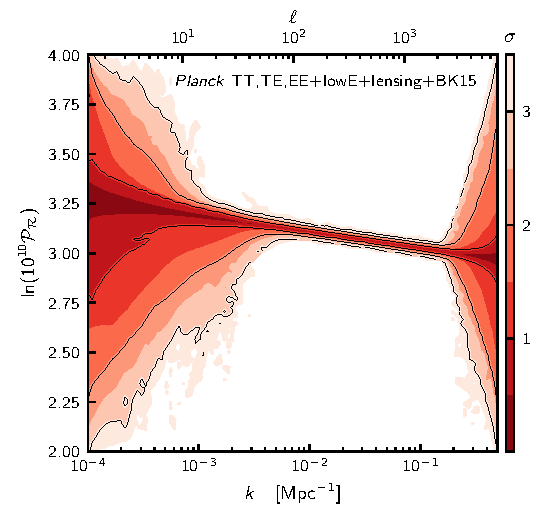
\includegraphics[width=0.7\textwidth]{figures/CMB_Power_Primordial.pdf}
\caption{Planck 2018による観測\cite{Planck:2018jri}。図は原始パワースペクトルへの制約を示す。これは$  4\% $の「赤い傾き」を除けばスケール不変である。\label{fig:scale}}
\end{figure}




インフレーションの最後の動機は、スケール不変性の問題である。観測は、原始摂動が、調べられるすべての宇宙論的尺度でほぼ同じ振幅をもつことを示す。等時刻相関関数の言葉では、スケール不変性は、すべての\(\lambda >0\)について
\begin{equation}
\langle \phi(x_1)\phi(x_2)\cdots \phi(x_n)\rangle
=
\langle \phi(\lambda x_1)\phi(\lambda x_2)\cdots \phi(\lambda x_n)\rangle .
\end{equation}
が成り立つことを意味する。特に、観測される二点関数はスケール不変に非常に近い。例えば図\ref{fig:scale}に示されている。これはきわめて驚くべきことである。例えばMinkowski時空の相関関数の計算から培われた一般的直観では、二点間の距離が離れると二点関数は減衰するはずだ。スケール不変性は相関が距離に依存しないと述べている。これは、明確な説明に値する、きわめて注目すべき事実である。



非常に魅力的なのは、この性質が、説明のつかない偶然ではなく、原始背景の対称性から従うという可能性である。簡単で美しい可能性は、初期宇宙が近似的にde Sitter時空
\begin{equation}
ds^2
=
-\frac{d\tau^2-dx^i dx^i}{H^2\tau^2}
=
-dt^2+e^{2Ht}dx^i dx^i ,
\end{equation}
で記述されることである。この時空は最大対称である。特に、平坦スライス表示のde Sitter時空は、拡大縮小の等長変換
\begin{equation}
\tau \to \lambda \tau,
\qquad
x^i \to \lambda x^i .
\end{equation}
を許す。他の背景量も少なくとも近似的にこの対称性を保つなら、原始相関関数の近似的なスケール不変性を自然に説明できる。以下では、時空がde Sitterでよく近似される期間が長く続いたと仮定する。






\subsection{長期間の準de Sitter膨張とその例}



上で概観した問題は、初期宇宙が、近似的にスケール不変な背景とともに、長期間の加速膨張を経験したことを示唆する。これらの性質をもつ時空はde Sitter時空
\begin{equation}
ds^2
=
-\frac{d\tau^2-dx^i dx^i}{H^2\tau^2}
=
-dt^2+e^{2Ht}dx^i dx^i ,
\end{equation}
であり、そのスケール因子は
\begin{equation}
a(\tau)=-\frac{1}{H\tau}=e^{Ht} .
\end{equation}
である。しかし、厳密なde Sitter時空は永遠に続くのに対し、インフレーションは終了しなければならない。したがって、Hubbleパラメータが時間とともにゆっくり変わる、近似的なde Sitter期を考えることになる。



加速膨張の条件を、次のように書き直すと有用である。
\begin{equation}
\frac{\ddot a}{a}=\dot H+H^2=H^2(1-\epsilon)>0 ,
\end{equation}
ここで\textit{第一Hubbleスローロールパラメータ}
\begin{equation}
\epsilon := -\frac{\dot H}{H^2} .
\end{equation}
を導入した。したがって、加速膨張には\(\epsilon<1\)が必要であり、準de Sitter段階は
\begin{equation}
0<\epsilon\ll 1 .
\end{equation}
に対応する。この条件は、宇宙が急速に膨張する間、\(H\)はゆっくりしか変わらないという考えを捉える。



第二の重要な要請は、インフレーションが十分長く続くことである。これを定量化するため、\textit{e-fold数}\(N\)を導入する。
\begin{equation}
dN := d\log a = H\,dt ,
\end{equation}
したがって、
\begin{equation}
N-N_0=\log\!\left(\frac{a}{a_0}\right) .
\end{equation}
である。地平線問題と曲率問題を解くには、十分長い加速膨張の期間
\begin{equation}
\Delta N_{\rm infl}:=N_e-N_i
>
50+\log\!\left(\frac{T_{\rm reh}}{10^{10}\,{\rm GeV}}\right) ,
\end{equation}
が必要である。$ T_{\rm reh}$は再加熱の終了時、すなわち高温ビッグバンの開始時の宇宙の温度である。現象論的に重要な再加熱温度については、これはしばしば
\begin{equation}
\Delta N_{\rm infl}\sim 25\text{--}60 .
\end{equation}
と要約される。概算では、単に\(\Delta N_{\rm infl}\sim 50\)を用いることが多い。



観測が数e-foldにわたる近似的なスケール不変性を示すので、インフレーション期全体を通じてde Sitterからのずれが小さいことを要求するのが自然である。これは、高次のHubbleスローロールパラメータ
\begin{equation}
\epsilon = -\partial_N\log H ,
\qquad
\eta = \frac{\dot\epsilon}{H\epsilon}=\partial_N\log\epsilon ,
\qquad
\xi_{n\ge 3}:=\partial_N\log\xi_{n-1} ,
\end{equation}
を用いて便利に表せる。ここで\(\xi_2\equiv \eta\)である。ある基準時刻\(N_\ast\)の周りで\(\epsilon(N)\)を展開すると、模式的に
\begin{align}
\epsilon(N)-\epsilon(N_\ast)
&=
\left.\frac{\partial\epsilon}{\partial N}\right|_{N_\ast}(N-N_\ast)
+\left.\frac{\partial^2\epsilon}{\partial N^2}\right|_{N_\ast}\frac{(N-N_\ast)^2}{2}
+\cdots
\nonumber\\
&=
\epsilon\left[
\eta(N-N_\ast)
+\eta(\eta+\xi_3)\frac{(N-N_\ast)^2}{2}
+\cdots
\right] .
\end{align}
となる。このことが、標準的なスローロール条件
\begin{equation}
\epsilon,\eta,\xi_n \ll 1 .
\end{equation}
を動機づける。これらの条件は、加速膨張だけでなく、背景が多数のe-foldにわたりde Sitterに近いままであることも保証する。このインフレーションの記述は、入門講義で出会うものと多少異なることに注意されたい。特に、まだスカラー場もポテンシャルも持ち出していない。さらに、スローロールパラメータはそれらの要素とは無関係であり、ここでは時空の性質としてのみ導入した。この意味で、ここまでの記述は、何がインフレーションを駆動したかについて特定の立場を取らない。\\



\paragraph{インフレーション模型の一群} 具体的な実現の広いクラスを、単一場の\(P(X,\phi)\)理論が与える。
\begin{equation}
S=\int d^4x\,\sqrt{-g}\left[\frac12 M_{\rm Pl}^2R+P(X,\phi)\right] ,
\end{equation}
ここで$ X$は、なじみ深い正準運動項
\begin{equation}
X:=-\frac12 g^{\mu\nu}\partial_\mu\phi\,\partial_\nu\phi
=
\frac12\left(\dot\phi^2-\frac{\partial_i\phi\,\delta^{ij}\partial_j\phi}{a^2}\right) .
\end{equation}
を表す。正準スカラー場は、特殊な場合
\begin{equation}
P(X,\phi)=X-V(\phi) .
\end{equation}
に対応する。\(R\phi^2\)のような、より一般的な非最小結合や、追加の微分を含む曲率結合は、ここでは論じない。



この作用から導かれるエネルギー運動量テンソルは
\begin{equation}
T_{\mu\nu}=P_{,X}\partial_\mu\phi\,\partial_\nu\phi+g_{\mu\nu}P(X,\phi) .
\end{equation}
である。これは、完全流体の形
\begin{equation}
T_{\mu\nu}=(\rho+p)u_\mu u_\nu + p\,g_{\mu\nu}
\end{equation}
を、次の同定のもとで取る。
\begin{equation}
\rho = 2X P_{,X}-P ,
\qquad
p = P ,
\qquad
u_\mu = -\frac{\partial_\mu\phi}{\sqrt{2X}} .
\end{equation}
したがって、\(P(X,\phi)\)理論は、一様な宇宙論的流体を場の理論で自然に実現する。



一様な背景\(\bar\phi(t)\)に注目すると、スカラー場の運動方程式は
\begin{equation}
\ddot{\bar\phi}\,\bigl(P_{,X}+2X P_{,XX}\bigr)
+
3H\dot{\bar\phi}\,P_{,X}
+
\bigl(2X P_{,X\phi}-P_{,\phi}\bigr)
=0 ,
\end{equation}
となり、Friedmann方程式と加速度方程式は
\begin{equation}
3M_{\rm Pl}^2H^2 = 2X P_{,X}-P ,
\qquad
- M_{\rm Pl}^2\dot H = X P_{,X} .
\end{equation}
となる。背景の詳細な発展は関数\(P\)の具体的な選択に依存するが、本稿の目的には、これらの方程式を具体的に解く必要はない。



第一スローロールパラメータが
\begin{equation}
\epsilon
=
\frac{3X P_{,X}}{2X P_{,X}-P} .
\end{equation}
と書けることに注意すれば十分である。これは、多くの\(P(X,\phi)\)の選択が、長く続くスローロール・インフレーション、すなわち\(\epsilon,\eta\ll 1\)という領域を支えうることを示す。この意味で、\(P(X,\phi)\)理論は、上述の準de Sitter的なインフレーション背景を動的に実現できる、簡単で柔軟な枠組みを与える。





\subsection{宇宙論とin-in相関関数}



ここでは、宇宙論で主に関心をもつ対象が、いわゆる宇宙論的相関関数、すなわち通常はインフレーションの終了時に取る、同時刻の局所演算子の積の期待値であることを説明する。幸い、これはまさにSchwinger--Keldysh形式が計算する対象である。本節では、純粋状態にある閉鎖系についてこの形式を説明する。これは文献の大部分で標準的に置かれる仮定である。次節では開放系と密度行列へ拡張し、摂動論の図式的なFeynman規則が本質的には同じであることを見る。\\





宇宙論では、次の形の期待値に関心がある。
\begin{equation}
\langle \Omega | \, O(\tau)\, | \Omega \rangle ,
\end{equation}
ここで\(O(\tau)\)は、同じ共形時刻\(\tau\)で評価した局所Heisenberg描像演算子の積であり、\(|\Omega\rangle\)は相互作用する真空を表す。インフレーションへの応用では、しばしば晩期極限
\begin{equation}
\tau \to 0^- ,
\end{equation}
に関心がある。de Sitter時空では、これは未来無限遠、あるいは等価に未来の共形境界に対応する。これは散乱理論で漸近時刻を\(\pm\infty\)に送ることの、自然な宇宙論版である。



このような相関関数の計算には、相互作用描像が便利である。閉じたユニタリ系のHamiltonianを、
\begin{equation}
\hat H(\tau)=\hat H_0(\tau)+\hat H_{\rm int}(\tau) .
\end{equation}
と分ける。自由部分\(\hat H_0\)が相互作用描像の場を定義し、\(\hat H_{\rm int}\)を摂動的に扱う。\(|0\rangle\)を自由真空とすると、相互作用する真空\(|\Omega\rangle\)は、無限の過去に相互作用を断熱的に入れることで得られる。その結果、期待値は
\begin{align}
\langle O(\tau)\rangle
&:=
\langle \Omega |\, O(\tau)\, | \Omega \rangle \\ \nonumber
&=
\frac{
\langle 0|\, \bar T \exp\!\left(i\int_{-\infty}^{\tau} d\tau' \,\hat H_{\rm int}(\tau')\right)
\, O(\tau)\,
T \exp\!\left(-i\int_{-\infty}^{\tau} d\tau' \,\hat H_{\rm int}(\tau')\right)
|0\rangle
}{
\langle 0|\, \bar T \exp\!\left(i\int_{-\infty}^{\tau} d\tau' \,\hat H_{\rm int}(\tau')\right)
T \exp\!\left(-i\int_{-\infty}^{\tau} d\tau' \,\hat H_{\rm int}(\tau')\right)
|0\rangle
} .
\end{align}
と書ける。\(T\)と\(\bar T\)は、それぞれ時間順序と反時間順序を表す。



相互作用する真空への正しい射影を実行すれば、分母は実際には1となる。この射影を正確に行うため、積分経路を複素平面内へわずかに変形する。最終結果は
\begin{equation}\label{inin-factorized}
\langle O(\tau)\rangle
=
\langle 0|
\left[
\bar T e^{\left(i\int_{-\infty(1+i\epsilon)}^{\tau} d\tau' \,\hat H_{\rm int}(\tau')\right)
}\right]
O(\tau)
\left[
T e^{ \left(-i\int_{-\infty(1-i\epsilon)}^{\tau} d\tau' \,\hat H_{\rm int}(\tau')\right)
}\right]
|0\rangle .
\end{equation}
である。経路の小さな虚方向への傾きにより、遠い過去の自由真空が相互作用する真空へ射影される。この表式は、密度行列を用いて単に
\begin{align}
\ex{O(\tau)}=\Tr(\rho(\tau) O(\tau))\,,
\end{align}
と書き直せる。ここで
\begin{align}
\rho(\tau)&=U(\tau,-\infty)\ket{0}\bra{0}U^{\dagger}(\tau,-\infty)\,,\\
U(\tau,-\infty)&=T \exp\!\left(-i\int_{-\infty(1-i\epsilon)}^{\tau} d\tau' \,\hat H_{\rm int}(\tau')\right)\,.
\end{align}
である。前節では、この演算子の表式をSK経路積分形式に翻訳した。以下では、演算子形式にとどまって調べる等価な方法を示す。これは宇宙論の文献でよく用いられ、\textit{in-in形式}と呼ばれる。二つの形式論のつながりをさらに明確にするために、これを行う。到達点は、摂動計算の図式的なFeynman規則の導出である。当然ながら、それらは演算子形式と経路積分形式のどちらで導いても同じである。\\



指数関数を摂動的に展開すると、
\begin{align} \nonumber
\langle O \rangle
&=
\Bigg\langle
\bar T
\left[
1+i\int H_{\rm int}
-\frac12\left(\int H_{\rm int}\right)^2+\cdots
\right]
O \,
T
\left[
1-i\int H_{\rm int}
-\frac12\left(\int H_{\rm int}\right)^2+\cdots
\right]
\Bigg\rangle ,
\end{align}
を得る。略記\(\int H_{\rm int}\)は\(\hat H_{\rm int}\)の適切な時間積分を表す。最初の数項を具体的に書くと、模式的に
\begin{align}\label{ptexp}
\langle O(\tau)\rangle
&=
\langle O(\tau)\rangle_0
+i\left\langle \int H_{\rm int}\, O(\tau)-O(\tau)\int H_{\rm int}\right\rangle_0
\\ \nonumber
&
-\frac12\left\langle
\left(\int H_{\rm int}\right)^2 O(\tau)
+O(\tau)\left(\int H_{\rm int}\right)^2
\right\rangle_0
+\left\langle
\left(\int H_{\rm int}\right) O(\tau)\left(\int H_{\rm int}\right)
\right\rangle_0
+\cdots ,
\end{align}
となる。\(\langle \cdots \rangle_0\)は自由真空での期待値を表す。これは摂動展開の\textit{因子化形式}と呼ばれることがある。





\paragraph{交換子形式} しばしばより便利な、等価な表現がある。これは
\begin{align}\label{inin-commutator}
\langle O(\tau)\rangle
&=
\sum_{N=0}^{\infty}
i^N
\int_{-\infty}^{\tau} d\tau_N
\int_{-\infty}^{\tau_N} d\tau_{N-1}
\cdots
\int_{-\infty}^{\tau_2} d\tau_1\\ 
& \quad \langle 0|\,
[\hat H_{\rm int}(\tau_1),
[\hat H_{\rm int}(\tau_2),
\ldots
[\hat H_{\rm int}(\tau_N),O(\tau)]
\ldots
]]
\,|0\rangle . \nonumber
\end{align}
と書ける。これがin-in摂動展開の\textit{交換子形式}である。最初の二つの次数を見ると、等価性が特に明瞭になる。ゼロ次では、
\begin{equation}\label{commutatorform}
\langle O(\tau)\rangle^{(0)}=\langle 0|\,O(\tau)\,|0\rangle .
\end{equation}
である。一次では、
\begin{align}
\langle O(\tau)\rangle^{(1)}
&=
\left\langle 0\left|
\left[i\int d\tau' \,\hat H_{\rm int}(\tau')\right] O(\tau)
+
O(\tau)
\left[-i\int d\tau' \,\hat H_{\rm int}(\tau')\right]
\right|0\right\rangle
\nonumber\\
&=
i\int_{-\infty}^{\tau} d\tau' \,
\langle 0|\, [\hat H_{\rm int}(\tau'),O(\tau)] \,|0\rangle .
\end{align}
となる。このように、因子化した公式の二つの枝が一つの交換子にまとまる。高次でも同じ仕組みによって、\eqref{inin-commutator}に現れる入れ子の交換子が生じる。\eqref{ptexp}との等価性は帰納法で証明できる\cite{Weinberg:2005vy}。



開放系の形式論を使うと、上の表式をうまく理解できる。まず、相互作用描像では密度行列が
\begin{align}
\rho'=-i[H_{\rm int},\rho]=:\L \rho\,,
\end{align}
に従うことを思い出そう。ここでLiouvillian超演算子$ \L$を導入した。形式解は
\[ \rho(\tau)=T \exp\left(  \int_{\tau_{0}}^{\tau}\L\right)\rho(\tau_{0})\,.\]
である。これをトレースに挿入すると、
\begin{align}
\ex{O(\tau)}&=\Tr\left(  \rho(\tau)O(\tau)\right)=\Tr\left(  T \exp\left(  \int_{\tau_{0}}^{\tau}\L\right)\rho(\tau_{0}) O(\tau)\right)\\
&=\Tr\left(  \rho(\tau_{0}) \bar T \exp\left(  \int_{\tau_{0}}^{\tau}\L^{\dagger}\right) O(\tau)\right)\,,
\end{align}
と書ける。随伴超演算子$ \L^{\dagger}$は、今度は$ O(\tau)$に$ i[H_{\rm int}, \dots]$として作用する。$ \tau_{0}\to-\infty$における純粋状態の初期条件$ \rho(\tau_{0})=\ket{0}\bra{0}$とトレースの巡回性を用いると、\eqref{inin-commutator}が再現される。




因子化形式\eqref{inin-factorized}と交換子形式\eqref{inin-commutator}は完全に等価だが、それぞれ異なる状況で有用である。因子化形式は図式的摂動論やSchwinger--Keldysh経路による記述に近い場合が多く、交換子形式は因果性と二つの枝の間の相殺をより明示する。実際には、考えている相関関数に最も便利な方を選べばよい。





\subsection{in-in相関関数のFeynman規則：$  \pm $基底}\label{sec5p4}



散乱振幅と同様、宇宙論的相関関数の摂動計算は、図式を使うと最も効率よく整理できる。得られる図式規則は、AdSのWitten図との類似を反映して、Feynman--Witten規則と呼ばれることもある。本節の残りは、\cite{Goodhew:2023bcu,PajerFieldTheoryCosmologyNotes}の議論にほぼ沿っている。



並進不変性により、運動量空間の任意の相関関数は、運動量保存を課すデルタ関数を一つ以上含む。複数のデルタ関数に比例する相関関数は非連結と呼ばれる。低点相関関数のあらゆる積を差し引くことで、全体で一つのデルタ関数をもつ連結部分が取り出される。連結相関関数については、
\begin{equation}
\left\langle \prod_{a=1}^n \phi(\mathbf k_a)\right\rangle_c
=
(2\pi)^3\delta^{(3)}\!\left(\sum_{a=1}^n \mathbf k_a\right)\,
B_n(\mathbf k_1,\dots,\mathbf k_n) .
\end{equation}
と書く。主な関心の対象は、この縮約相関関数\(B_n\)である。



\(B_n\)の摂動規則は、前小節で論じた展開に現れる相互作用描像の演算子について、可能なWick縮約をすべて行うだけで導かれる。この閉鎖系の設定では時間発展がHamilton的なので、まもなく見るように、最終的なFeynman規則には、経路積分のプラス・マイナス基底による自然な解釈がある。次節では、経路積分から出発して開放系へ一般化し、遅延場と先進場の言葉で等価なFeynman規則を展開する。



\begin{enumerate}
\item
\(n\)点相関関数について、晩期境界\(\tau\to 0\)で終わる\(n\)本の外線、バルクの相互作用頂点\(V\)個、および頂点対を結ぶ内線\(I\)本をもつすべての図を描く。時間は無限の過去\(\tau\to-\infty\)から未来の共形境界\(\tau\to 0\)へ流れる。



\item
各相互作用頂点は、in-in経路のどちらの枝にも置ける。そこで、各頂点に、時間順序付き時間発展演算子に対応する\(+\)頂点、または反時間順序付き時間発展演算子に対応する\(-\)頂点というラベルを付ける。\(V\)個の頂点への\(+\)／\(-\)ラベルの\(2^V\)通りの割り当てすべてについて和を取る。



\item
各外線に、\(a=1,\dots,n\)として運動量\(\mathbf k_a\)を割り当て、すべてバルク頂点から未来境界へ流れるものとする。各内線には、\(m=1,\dots,I\)として積分運動量\(\mathbf p_m\)を割り当て、これらの運動量すべてについて積分する。



\item
各バルク頂点について、その頂点の時刻\(\tau_i\)で評価した対応する相互作用Hamiltonian密度と、\(\tau_i\)についての積分を含める。\(+\)頂点は因子
\begin{equation}
-i\int_{-\infty(1-i\epsilon)}^0 d\tau_i\, H_{\rm int}(\tau_i),
\end{equation}
を与え、\(-\)頂点は
\begin{equation}
+i\int_{-\infty(1+i\epsilon)}^0 d\tau_i\, H_{\rm int}(\tau_i).
\end{equation}
を与える。逆の符号と逆の\(i\epsilon\)処方は、これらの項が、ブラとケットの時間発展における$ U$と$ U^{\dagger}$に由来することを反映する。Schwinger--Keldysh経路積分の言葉では、これらが閉時間経路の二つの枝である。



\item
時刻\(\tau_i\)のバルク頂点と時刻\(\tau=0\)の境界演算子を結ぶ各外線に、適切なバルク・境界伝播子$  G_{\pm} $を挿入する。具体的には、場の演算子を自由モードで
\begin{equation}
\phi_{\mathbf k}(\tau)=u_k(\tau)a_{\mathbf k}+u_k^*(\tau)a^\dagger_{-\mathbf k},
\end{equation}
と展開すると、外線は、\(+\)頂点と\(-\)頂点のどちらに接続するかに応じて、\(u_k(\tau_i)\)または\(u_k^*(\tau_i)\)を与える。
\begin{equation}
G_+(k;\tau_i,0)=u_k(\tau_i)\,u_k^*(0),
\qquad
G_-(k;\tau_i,0)=u_k^*(\tau_i)\,u_k(0) .
\end{equation}



\item
時刻\(\tau_i\)と\(\tau_j\)の頂点を結ぶ各内線に、対応する相互作用描像の場の間の自由な二点縮約を挿入する。具体的な伝播子は、二つの端点が経路の同じ枝にあるか、異なる枝にあるかに依存する。
\begin{align}
G_{++}(\tau_i,\tau_j;\mathbf p) &= \langle T\,\phi_{\mathbf p}(\tau_i)\phi_{-\mathbf p}(\tau_j)\rangle,\\
G_{--}(\tau_i,\tau_j;\mathbf p) &= \langle \bar T\,\phi_{\mathbf p}(\tau_i)\phi_{-\mathbf p}(\tau_j)\rangle,\\
G_{+-}(\tau_i,\tau_j;\mathbf p) &= \langle \phi_{-\mathbf p}(\tau_j)\phi_{\mathbf p}(\tau_i)\rangle,\\
G_{-+}(\tau_i,\tau_j;\mathbf p) &= \langle \phi_{\mathbf p}(\tau_i)\phi_{-\mathbf p}(\tau_j)\rangle .
\end{align}
同じ情報が遅延・先進・Keldysh伝播子に符号化される\(r/a\)基底での方法を、後に見る。



\item
各頂点で運動量保存を課す。すべての頂点のデルタ関数を用いた後には、連結相関関数に要求されるとおり、全体の因子
\begin{equation}
(2\pi)^3\delta\!\left(\sum_{a=1}^n \mathbf k_a\right)
\end{equation}
が一つ残る。



\item
図の適切な対称性因子で割る。詳細は\cite{Goodhew:2023bcu,PajerFieldTheoryCosmologyNotes}を参照。



\item
最後に、異なるすべての図と、\(+\)／\(-\)ラベルのすべての割り当てについて和を取る。
\end{enumerate}



これらの規則は、通常のFeynman規則の宇宙論版である。主な新しさは、二重化した経路構造にあり、\(+\)頂点と\(-\)頂点を区別し、対応する伝播子と符号を追跡する必要がある。実際には、in-in展開の因子化形式は自然に\(+\)／\(-\)基底を導き、一方、因果的性質を整理し半古典極限を調べるには、\(r/a\)基底の方が効率的な場合が多い。



これらの規則の適用例は、\cite{PajerFieldTheoryCosmologyNotes}に多数ある。ここでは繰り返さず、主に研究する理論のクラスの導入へ進む。





\subsection{原始非ガウス性とバイスペクトル}



ガウス確率場は、その二点関数によって完全に特徴づけられる。等価に、二点関数を超えるすべての連結相関関数はゼロとなり、高次の偶数点関数全体は、Wickの定理によって二点関数から決まる。したがって、非ガウス性は二点関数を超える連結相関関数に符号化され、その最初の例が三点関数、あるいはバイスペクトルである。ここでは、しばしば原始非ガウス性と呼ばれる、インフレーション中に生成された非ガウス性の研究の主要な側面を簡潔に論じ、まとめる。\\



統計的に一様な場\(\zeta\)の任意の連結\(n\)点関数に対し、並進不変性から運動量空間での形
\begin{equation}
\langle \zeta_{\mathbf k_1}\zeta_{\mathbf k_2}\cdots \zeta_{\mathbf k_n}\rangle
=
(2\pi)^3\delta^{(3)}\!\left(\mathbf k_1+\mathbf k_2+\cdots+\mathbf k_n\right)\,
B_n(\mathbf k_1,\mathbf k_2,\dots,\mathbf k_n) .
\end{equation}
が従う。全体のデルタ関数は運動量保存を課し、縮約相関関数\(B_n\)が物理的情報を含む。\(n\)個の運動量は\(3n\)個の実成分をもち、並進不変性がそのうち三つを取り除く。回転不変性がさらに三つを取り除く。したがって、追加の対称性を課す前には、縮約\(n\)点関数は、$ n\geq 3$について$ 3n-6  $個の独立変数に依存する。



場が近似的にスケール不変なら、相関関数は
\begin{equation}
\langle \zeta(\lambda \mathbf x_1)\zeta(\lambda \mathbf x_2)\cdots \zeta(\lambda \mathbf x_n)\rangle
=
\langle \zeta(\mathbf x_1)\zeta(\mathbf x_2)\cdots \zeta(\mathbf x_n)\rangle ,
\end{equation}
あるいは等価に運動量空間では、
\begin{equation}
B_n(\lambda \mathbf k_1,\lambda \mathbf k_2,\dots,\lambda \mathbf k_n)
=
\lambda^{-3(n-1)}B_n(\mathbf k_1,\mathbf k_2,\dots,\mathbf k_n) .
\end{equation}
を満たす。したがって、スケール不変性がさらに一つの自由度を取り除き、$ 3n-7  $個の独立変数が残る。



\paragraph{バイスペクトル} 特に、バイスペクトル\(B_3\)では、最も一般的な回転不変な配置は三つの数で指定される。それらは三角形の三辺の長さ
\begin{equation}
k_1:=|\mathbf k_1|,
\qquad
k_2:=|\mathbf k_2|,
\qquad
k_3:=|\mathbf k_3|,
\qquad
\mathbf k_1+\mathbf k_2+\mathbf k_3=0 .
\end{equation}
と取れる。さらにスケール不変性を仮定すると、独立な形状変数は二つだけ残り、例えば比\(k_2/k_1\)と\(k_3/k_1\)\cite{Babich:2004gb}を選べる。



各挿入で場\(\zeta\)は同一なので、バイスペクトルは\(k_1\)、\(k_2\)、\(k_3\)の置換についても対称である。したがって、バイスペクトルを、置換で同一視した運動量三角形の空間上の関数と考えるのが自然である。しばしば、全体の振幅と三角形の形への依存を、
\begin{equation}
B_3(k_1,k_2,k_3)=A\,\frac{S(k_1,k_2,k_3)}{(k_{1}k_{2}k_{3})^{2}} ,
\end{equation}
と書いて分離する。\(A\)は全体の振幅、\(S\)は形状関数である。規格化した形状関数は、特定の配置での値を固定することで定義できる。例えば、正三角形配置で
\begin{equation}
S(k,k,k)=1
\end{equation}
を要求する。このようにして、振幅と三角形の形への依存が明確に分離される。文献ではさまざまな規格化条件が使われているため、$ A  $の値についての議論を解釈する前に、規約を確認する必要がある。\\



異なる物理機構は、三角形空間の異なる領域でピークをもつバイスペクトルを生成する。したがって、いくつかの特殊な極限に注目すると、議論を整理しやすい。



第一は\textit{スクイーズ極限}である。
\begin{equation}
k_1 \ll k_2 \simeq k_3 .
\end{equation}
これは、一つの長波長モードと二つの短波長モードの結合を調べる。この極限で大きいバイスペクトルは、長短モード間の強い結合を示す。単純な単一時計のアトラクター模型では、この極限は強く制約される\cite{Maldacena:2002vr,Creminelli:2004yq,Flauger:2013hra,Creminelli:2011sq,Hinterbichler:2012nm,Hinterbichler:2013dpa,Creminelli:2012ed,Pajer:2013ana,Dai:2015rda,Creminelli:2013cga,Cabass:2016cgp,Pajer:2017hmb,Finelli:2017fml}。一方、スクイーズ配置で大きな信号があれば、インフレーション中の追加の軽い自由度の存在、あるいはより一般に、最も単純な単一場の断熱的描像からのずれを示唆しうる。



第二は\textit{正三角形極限}である。
\begin{equation}
k_1=k_2=k_3 .
\end{equation}
この配置は、インフラトン・セクターの微分自己相互作用によって自然に強調される。後で見るように、デカップリング極限のインフレーション有効場理論は、まさにこの型の非ガウス性を生む。



第三は、平坦化した極限、あるいは\textit{折り畳み極限}である。
\begin{equation}
k_1+k_2=k_3 ,
\end{equation}
ここでは置換を同一視する。この場合、運動量三角形の面積はゼロへ近づく。このような配置でピークをもつ信号は、標準的でない物理効果、例えば非自明な初期状態\cite{Holman:2007na,Agarwal:2012mq}、あるいは後で論じるインフレーション有効理論の開放系効果\cite{LopezNacir:2011kk,Salcedo:2024smn,Salcedo:2026sdn,Green:2020whw,Creminelli:2023aly}から生じうる。



標準的なインフレーション有効場理論が、主として正三角形型のバイスペクトルを予言することを見る。その後、折り畳み極限への寄与が一般に生じるインフレーションの開放有効理論で、この描像がどう変わるかを調べる。





\section{インフレーションの開放有効場理論}\label{sec:6}



ここで、これまで展開してきた二つの主題、インフレーションと開放量子系の一般的枠組みを結びつける準備が整った。インフレーションへのユニタリな有効場理論（EFT）のアプローチでは、破れた時間並進に対応するGoldstoneボソンに注目し、その動力学を、重力に結合していてもよい閉鎖系として調べる。しかし実際には、観測可能なセクターは、重い、短寿命である、あるいは別の理由でアクセスできない追加の自由度と相互作用しうる。したがって、Goldstoneモードを、未知の環境と相互作用する開放系として扱うと、インフレーションの動力学がどう変わるかを問うのは自然である。本節の目的は、対応する開放有効場理論を構築し、その主要な観測的帰結を調べることである。



最初の二つの小節での目標は、重力を固定された非動的な背景とし、場$ \pi$だけのインフレーションEFT、\eqref{goal}を導くことである。この目標には、まず平坦時空で、自発的に破れた時間並進に対応するGoldstoneボソン$ \pi$の理論を構築し、それを固定したFLRW背景時空に最小結合すればよい。第\ref{sec:6p1}節で概説するこの方法は非常に直観的だが、背景のEinstein方程式からWilson係数に課される制約の一部を見落とす。より長いが正確な導出は、時間微分同相変換が自発的に破れた、計量だけの一般理論から始まる。そこでは、$ \pi$は理論を四次元微分同相不変にするSt\"uckelberg場として現れる。その後、$ \pi$と計量揺らぎのデカップリングを用いて、最終的な作用\eqref{goal}を得る。



続いて、場を二重化し、非平衡の整合性条件を課し、Schwinger--Keldysh経路上で大域対称性がどうなるかを論じ、得られる理論を遅延・先進基底で整理することで、この構成を開放系へ一般化する。最後に、二次理論、その伝播子とパワースペクトルを調べ、三次相互作用とバイスペクトルへ進む。これにより、開放的なインフレーション動力学の特徴的な兆候、特に折り畳み配置近傍での信号の増強を同定できる。





\subsection{平坦空間における、破れた時間並進のGoldstoneボソン}\label{sec:6p1}



重力のあるインフレーション有効場理論を導入する前に、平坦時空の、より簡単な非重力系を考えると有用である\footnote{本小節は、\cite{Finelli:2018upr}の議論に沿って、インフレーションEFT\cite{Creminelli:2006xe,Cheung:2007st}の構成を導入する。}。この準備の目的は、時間並進の自発的破れに伴うGoldstoneモードの出現の背後にある、対称性の論理を取り出すことである。



最も一般的な局所Lagrangian
をもつ、単一スカラー場\(U(x)\)のPoincar\'e不変な理論を考える。
\begin{equation}
\mathcal L=\mathcal L\bigl(U,\partial_\mu U,\partial_\mu\partial_\nu U,\dots\bigr) .
\end{equation}
この理論が、一様だが時間に依存する背景解\(\bar U(t)\)をもつとする。その周りの摂動は、次のようにパラメータ化すると便利である。
\begin{equation}
U(x)=\bar U\bigl(t+\pi(x)\bigr).
\end{equation}
場\(\pi(x)\)は、時間並進の自発的破れに対応するGoldstoneボソンである。これは破れた時空対称性のもとで\textit{非線形に変換}する。



Poincar\'e変換\(x^\mu\to \Lambda^\mu{}_\nu x^\nu+\alpha^\mu\)のもとで、スカラー場\(U(x)\)は線形に変換するが、Goldstone場\(\pi\)は非線形に変換する。結果を具体的に書くと、
\begin{equation}\label{Poincareonpi}
\pi(x)\to \pi(\Lambda x+\alpha)+\alpha^0+\Lambda^0{}_\mu x^\mu-t .
\end{equation}
となる。この表式は、背景が時間並進とブーストを破り、一方、空間並進と回転は線形に実現されたままであることを明示する。この非線形変換は、よりなじみ深い共変スカラー場の変換
\[ \phi(x) \to \phi(\Lambda x +\alpha) \,, \]
と対比すべきである。後者では、変換後の表式が場$  \phi $について\textit{線形}である。この構造が、自発的対称性の破れの特徴である。



\(\pi\)の有効作用は、非線形に実現されるこれらの対称性と両立する最も一般的な局所作用を、微分展開として整理して書くことで得られる。\(\bar U(t)\)が単調だと仮定すれば、常に場を再定義して
\begin{equation}
\bar U(t)=t .
\end{equation}
とできる。このとき、微分の最低次で、最初の共変な構成要素は
\begin{equation}
\partial_\mu U\,\partial^\mu U 
=
-1-2\dot\pi+\partial_\mu\pi\,\partial^\mu\pi .
\end{equation}
である。上の構成要素に1を加えて背景を取り除き、摂動の一次から始まる量にすると便利な場合が多い。
第二の共変な構成要素は$ U=t+\pi$であり、Wilson係数は$  (t+\pi(t,{\bf x})) $の任意の関数でよい。\eqref{Poincareonpi}のように$  \pi $に作用する任意のPoincar\'e変換に対して、
\begin{align}
t+\pi(t,{\bf x})\to t'+\pi(t',{\bf x}')\,.
\end{align}
が成り立つ。有効作用を構築する際、すべてのWilson係数は$  (t+\pi(t) ) $の任意の関数でよい。したがって、場一つ当たり高々一つの微分を含む項まででは、有効作用は次の形を取る。
\begin{equation}
S
=
\int d^4x\,
\sum_{n=0}^{\infty}
\frac{d_n(t+\pi)}{n!}
\Bigl(-2\dot\pi+\partial_\mu\pi\,\partial^\mu\pi\Bigr)^n .
\end{equation}
より一般には、高階微分演算子も含められる。本論文の記法に従うと、有用な例の一つが量
\begin{equation}
K
=
\frac{\Box U}{\sqrt{-\partial_\mu U\partial^\mu U}}
+
\frac{\partial^\mu U\,\partial^\nu U\,\partial_\mu\partial_\nu U}
{\bigl(-\partial_\mu U\partial^\mu U\bigr)^{3/2}} ,
\end{equation}
であり、\(\pi\)の二次まででは、
\begin{equation}
K
=
-\partial_i\partial_i\pi
+\dot\pi\,\partial_i\partial_i\pi
+2\,\partial_i\pi\,\partial_i\dot\pi
+\mathcal O(\pi^3) .
\end{equation}
となる。このような項を含めると、有効作用は
\begin{equation}
S_{\rm h.d.}=
\int d^4x
\sum_{n=0}^{\infty}
\frac{\hat d_n(t+\pi)}{n!}
\Bigl(-2\dot\pi+\partial_\mu\pi\,\partial^\mu\pi\Bigr)^n K
+\cdots
\end{equation}
と書ける。以下では、これらの高階微分項を省略する。



二つの事実が明らかになるように作用を書き直すと有用である。第一に、タドポールの相殺により、作用は摂動の二次から始まる。第二に、係数が時間に依存しない場合、Goldstoneモードはゼロ運動量でデカップルし、等価に\(\pi={\rm const}\)は常に解である。この形では、
\begin{align}
S=
\int d^4x\,
\Bigg[
&d_1(t+\pi)\,\partial_\mu\pi\,\partial^\mu\pi
+
\sum_{n=2}^{\infty}
\frac{d_n(t+\pi)}{n!}
\Bigl(-2\dot\pi+\partial_\mu\pi\,\partial^\mu\pi\Bigr)^n\Bigg]
\end{align}
を得る。この作用は、時間並進とブーストを自発的に破る任意の平坦空間の系について、微視的詳細に依存しない、普遍的な低エネルギーセクターを記述する。



宇宙論への教訓は明らかである。どの宇宙論でも、一様な背景は時間並進を破るため、対応するGoldstoneボソンは、やはり時計変数をずらすことで導入される。主な違いは、重力系では時間並進が微分同相不変性の一部であるため、ユニタリゲージを固定してからSt\"uckelberg場で時間微分同相変換を復元すると、Goldstoneモードが最も自然に導入されることである。上の平坦空間の構成は、重力の追加の複雑さなしにこの論理を見る、最も簡単な設定を与える。





\subsection{デカップリング極限のインフレーションEFT}



ここで、具体的な計算を行う理論のクラス、インフレーションの有効場理論を導入する。本小節では終始、ユニタリな閉鎖系理論に限定し、場当たりの微分数が最小の演算子だけを残す。特に、外的曲率や高階微分の幾何学的量を含む演算子は無視する。



概念的な出発点は、インフレーション背景が、背景の時計場が一定の面という、時空の特定のスライスを選ぶことである。その結果、時間微分同相変換は背景によって自発的に破れるが、空間微分同相変換は破れない。したがって、有効場理論は、空間微分同相変換だけを保つ幾何学的量から構成される、最も一般的な作用となる。



時間微分同相変換を利用し、時計場の揺らぎをゼロにして、すべてのスカラー摂動を計量に符号化することができる。これを\textit{ユニタリゲージ}と呼ぶ。このゲージでは、理論は単に、時間依存する空間微分同相変換には不変だが、時間微分同相変換には必ずしも不変でない時空計量の理論として記述される。最低微分数のセクターに限れば、作用は
\begin{equation}\label{EFTI-unitary}
S
=
\int d^4x\,\sqrt{-g}\,
\left[
\frac{M_{\rm Pl}^2}{2}R
+d_0(t)
+d_1(t)\,\delta g^{00}
+\sum_{n=2}^{\infty}\frac{d_n(t)}{n!}\bigl(\delta g^{00}\bigr)^n
\right] ,
\end{equation}
の形を取る。ここでは宇宙時刻$  t $を用いるので$  \bar g_{00}=-1 $であり、背景の寄与を、次の定義で取り除いた。
\begin{equation}
\delta g^{00}:=g^{00}-\bar g^{00}=g^{00}+1 .
\end{equation}
Einstein--Hilbert項に続く最初の二項はタドポールである。その役割は、選んだFLRW背景が運動方程式を解くようにすることだけである。したがって、それらは背景の発展から決まり、独立な相互作用係数ではない。



平坦なFLRW背景
\begin{equation}
ds^2=-dt^2+a(t)^2\,d\mathbf x^2 ,
\end{equation}
に対して、タドポール係数はFriedmann方程式で固定される。これらを次のように書き直すと便利である。
\begin{equation}
d_0(t)=-M_{\rm Pl}^2\bigl(3H^2+2\dot H\bigr),
\qquad
d_1(t)=M_{\rm Pl}^2\dot H ,
\end{equation}
すると作用は
\begin{equation}\label{EFTI-unitary-standard}
S
=
\int d^4x\,\sqrt{-g}\,
\left[
\frac{M_{\rm Pl}^2}{2}R
-M_{\rm Pl}^2(3H^2+\dot H)
+M_{\rm Pl}^2\dot H\,g^{00}
+\sum_{n=2}^{\infty}\frac{d_n(t)}{n!}\bigl(\delta g^{00}\bigr)^n
\right] .
\end{equation}
となる。微分の最低次では、最小のスローロール理論からのあらゆるずれは、係数\(d_n(t)\)に符号化される。



この作用を直接用いてもよいが、通常の一般相対論の扱いとつながるように、四次元の微分同相変換全体に不変な形へ書き直すと非常に便利である。これはSt\"uckelbergの手法で実現できる。しかし、まもなく見るように、この手法はさらに多くのことを明らかにする。追加のスカラー自由度の存在と、それが重力揺らぎからデカップルする高エネルギー領域を明示するのである。



具体的には、理論の新たな場となるゲージパラメータ$  \pi(x) $を用いて、破れた時間微分同相変換
\begin{equation}
t\to t+\pi(x) .
\end{equation}
を行う。\(\pi(x)\)を、破れた時間並進に対応するGoldstoneボソンと解釈する。この変換のもとで、計量成分\(g^{00}\)は非線形に変換する。
\begin{equation}\label{Deltadeltag00}
\delta g^{00}
\;\to\;
\delta g^{00}
+2g^{0\mu}\partial_\mu \pi
+g^{\mu\nu}\partial_\mu \pi\,\partial_\nu \pi\,.
\end{equation}


\paragraph{デカップリング極限} 特に有用な簡略化が\emph{デカップリング極限}である。完全な理論では、インフレーション背景が時間微分同相変換を破るため、Goldstoneモード\(\pi\)は計量揺らぎと混合する。しかし、十分高いエネルギーでは、この混合は無視でき、摂動のないFLRW背景上で\(\pi\)の動力学だけを調べられる。具体的には、計量を一様背景の値で評価し、ラプス、シフト、空間計量の揺らぎを残さず、置換\(t\to t+\pi(x)\)によってGoldstone場を復元する。得られる作用は、主要なスカラー動力学を捉えつつ、計算を大幅に簡単にする。



デカップリング極限は、\(H\)程度以上のエネルギーで信頼できると期待される。物理的には、\(\pi\)と重力の混合が、背景のゆっくりした時間依存性を支配するのと同じ尺度で制御される一方、保持する\(\pi\)の自己相互作用はこの領域で抑制されないためである。したがって、デカップリング極限からのずれはスローロールで抑制され、本稿の仮定のもとでは、保持する主要効果よりパラメトリックに小さい補正を生むと期待される。この極限では、変換\eqref{Deltadeltag00}を、摂動のないFLRW計量で単に評価すればよい。その結果、
\begin{equation}\label{dg00-Stuck}
\delta g^{00}
\;\to\;
-2\dot\pi-\dot\pi^2+\frac{(\partial_i\pi)^2}{a^2} .
\end{equation}
を得る。この一つの置換だけで、必要な次数までのGoldstone作用を決められる。\eqref{dg00-Stuck}を\eqref{EFTI-unitary-standard}に代入し、\(\pi\)の三次まで展開すると、
\begin{align}\label{goal}
S_\pi
=
\int d^4x\,a^3
\Bigg[
&-M_{\rm Pl}^2\dot H
\left(
\dot\pi^2-\frac{(\partial_i\pi)^2}{a^2}
\right)
+2d_2\,\dot\pi^2
\nonumber\\
&\qquad
+\left(2d_2-\frac{4}{3}d_3\right)\dot\pi^3
-2d_2\,\dot\pi\,\frac{(\partial_i\pi)^2}{a^2}
+\cdots
\Bigg] .
\end{align}
を得る。省略記号は、高次の項と、デカップリング極限の展開で抑制される項を表す。



二次作用を音速\(c_s\)でパラメータ化するのが慣例である。最初の二つの二次項をまとめると、
\begin{equation}
S_\pi^{(2)}
=
\int d^4x\,a^3
\left[
-M_{\rm Pl}^2\dot H\,c_s^{-2}\,\dot\pi^2
+M_{\rm Pl}^2\dot H\,\frac{(\partial_i\pi)^2}{a^2}
\right] ,
\end{equation}
と書ける。ここで
\begin{equation}\label{cs-def}
\frac{1}{c_s^2}
=
1-\frac{2d_2}{M_{\rm Pl}^2\dot H} .
\end{equation}
である。インフレーション中は\(\dot H<0\)なので、安定な理論では運動項の係数は正である。



\eqref{cs-def}を用いると、二次作用は
\begin{equation}
S_\pi^{(2)}
=
\int d^4x\,a^3
\left[
-M_{\rm Pl}^2\dot H
\left(
\frac{1}{c_s^2}\dot\pi^2-\frac{(\partial_i\pi)^2}{a^2}
\right)
\right] .
\end{equation}
となる。これは、非自明な係数\(d_2\)が、Goldstoneモードの伝播速度を相対論的な値\(c_s=1\)から変えることを示す。



三次では、主要な二つの相互作用は
\begin{equation}\label{EFTI-cubic}
S_\pi^{(3)}
=
\int d^4x\,a^3
\left[
\left(2d_2-\frac{4}{3}d_3\right)\dot\pi^3
-2d_2\,\dot\pi\,\frac{(\partial_i\pi)^2}{a^2}
\right] .
\end{equation}
である。\(\delta g^{00}\)のべきから構成される最低微分数のEFTに限定すると、演算子\(\dot\pi(\partial_i\pi)^2\)は理論への独立した追加ではない。むしろ、置換\eqref{dg00-Stuck}を決めたのと同じ、非線形に実現される対称性によって固定される。特に、二次の運動項、したがって音速を変えるのと同じ演算子\((\delta g^{00})^2\)から生じる。このため、その係数は\(c_s\)によって決まる一方、\(\dot\pi^3\)の係数は次のEFTパラメータ\(d_3\)にも依存する。



\eqref{cs-def}を使うと、混合した三次相互作用は
\begin{equation}
-2d_2\,\dot\pi\,\frac{(\partial_i\pi)^2}{a^2}
=
-M_{\rm Pl}^2\dot H
\left(1-\frac{1}{c_s^2}\right)
\dot\pi\,\frac{(\partial_i\pi)^2}{a^2} .
\end{equation}
と書ける。したがって、音速を下げると、この相互作用は自動的に増強される。



最後に、Goldstoneモード\(\pi\)は、一次では曲率摂動\(\zeta\)と直接関係している。
\begin{equation}
\zeta = -H\pi + \cdots ,
\end{equation}
したがって、上の作用は、観測可能なスカラー摂動のインフレーション相関関数を計算する出発点を与える。次の小節では、先に展開したin-in形式を使い、\eqref{EFTI-cubic}の三次相互作用が生成する相関関数を評価する。






\subsection{主要なEFT演算子が生む原始非ガウス性}



ここでは、デカップリング極限のインフレーションEFTにおける、主要な二つの三次相互作用
が生成する木レベルのバイスペクトルを計算する。
\begin{equation}
S_\pi^{(3)}
=
\int d^4x\,a^3
\left[
C_{\dot\pi^3}\,\dot\pi^3
+
C_{\dot\pi(\partial\pi)^2}\,
\dot\pi\,\frac{(\partial_i\pi)^2}{a^2}
\right] ,
\end{equation}
ここで
\begin{equation}
C_{\dot\pi(\partial\pi)^2}
=
-\,M_{\rm Pl}^2\dot H\left(1-\frac{1}{c_s^2}\right) ,
\end{equation}
であり、\(C_{\dot\pi^3}\)は前小節で論じたように、次のEFT係数に依存する。



これらの純粋にユニタリな木レベル計算では、\(+\)／\(-\)基底が最も簡潔である。答えが、\(+\)の接触図と\(-\)の接触図の和になるだけだからである。\(r/a\)基底で対応する計算をすることも可能だが、相互作用が複数の項に分かれるので簡潔さに欠ける。対照的に、後の開放系の設定では、\(r/a\)基底がはるかに有用になる。



この次数では、バルク・境界伝播子だけが必要である。Goldstone場の、質量ゼロの自由なde Sitterモード関数
\begin{equation}
u_k(\tau)
=
\frac{i}{2M_{\rm Pl}\sqrt{\epsilon c_s\,k^3}}
\left(1+ikc_s\tau\right)e^{-ikc_s\tau} ,
\end{equation}
を用いると、バルク・境界伝播子は
\begin{equation}
G_{+}(k;\tau)
:=
u_k(\tau)\,u_k^*(0) =G_{-}(k;\tau)^{\ast}.
\end{equation}
となる。その時間微分と空間微分も必要である。
\begin{equation}
\partial_\tau u_k(\tau)
=
-\frac{i}{2M_{\rm Pl}\sqrt{\epsilon c_s\,k^3}}\,
c_s^2k^2\tau\,e^{-ikc_s\tau},
\qquad
\partial_i \to ik_i
\quad
\text{Fourier 空間で}.
\end{equation}
最後に、一次では
\begin{equation}
\zeta=-H\pi ,
\end{equation}
なので、\(\pi\)の三点関数を計算すれば、対応する\(\zeta\)のバイスペクトルが直ちに得られる。



\(+\)と\(-\)の接触図は互いに複素共役なので、全結果は\(+\)の寄与の実部の2倍である。等価に、
\begin{equation}
\langle \zeta_{\mathbf k_1}\zeta_{\mathbf k_2}\zeta_{\mathbf k_3}\rangle'
=
2\,\mathrm{Re}\left[
-i
\int_{-\infty(1-i\epsilon)}^0 d\tau\,
\langle
\zeta_{\mathbf k_1}(0)\zeta_{\mathbf k_2}(0)\zeta_{\mathbf k_3}(0)\,
H_{\rm int}(\tau)
\rangle
\right] ,
\end{equation}
と書ける。プライムは、全体の運動量保存デルタ関数を取り除いたことを表す。小さな\(i\epsilon\)の傾きが、\(\tau\to-\infty\)での収束を保証する。



\paragraph{\(\dot\pi^3\)相互作用。}
次の場合、
\begin{equation}
H_{\rm int}^{\dot\pi^3}(\tau)
=
-\int d^3x\,a^3\,C_{\dot\pi^3}\,\dot\pi^3 ,
\end{equation}
スケール因子の因子が三つの時間微分と相殺されるため、\(+\)図は
\begin{equation}
-i\,C_{\dot\pi^3}
\int_{-\infty(1-i\epsilon)}^0 d\tau\,
\partial_\tau G_{+}(\tau,k_1)\,
\partial_\tau G_{+}(\tau,k_2)\,
\partial_\tau G_{+}(\tau,k_3) .
\end{equation}
に比例する。具体的なモード関数を使えば、時間積分は初等的に実行でき、
\begin{equation}
B_\zeta^{\dot\pi^3}(k_1,k_2,k_3)
=
\mathcal A_{\dot\pi^3}\,
\frac{1}{(k_1k_2k_3)^3}\,
S_{\dot\pi^3}(k_1,k_2,k_3) ,
\end{equation}
を得る。\(\mathcal A_{\dot\pi^3}\)は\(C_{\dot\pi^3}\)、\(H\)、\(\epsilon\)、\(c_s\)、\(M_{\rm Pl}\)に依存する全体の振幅であり、
\begin{equation}
S_{\dot\pi^3}(k_1,k_2,k_3)
=
\frac{k_1^2k_2^2k_3^2}{k_{T}^3},
\qquad
k_{T}:=k_1+k_2+k_3 .
\end{equation}
である。三つの運動量の長さの対称な組み合わせ$  k_{T} $は、\textit{全エネルギー}として知られる。したがって、\(\dot\pi^3\)が生成する形状は、三つの運動量が同程度の場合に大きくなる。



\paragraph{\(\dot\pi(\partial_i\pi)^2\)相互作用。}
次の場合、
\begin{equation}
H_{\rm int}^{\dot\pi(\partial\pi)^2}(\tau)
=
-\int d^3x\,a^3\,
C_{\dot\pi(\partial\pi)^2}\,
\dot\pi\,\frac{(\partial_i\pi)^2}{a^2},
\end{equation}
スケール因子は再び相殺され、\(+\)の接触図は
\begin{equation}
-i\,C_{\dot\pi(\partial\pi)^2}
\int_{-\infty(1-i\epsilon)}^0 d\tau\,
\left[
\partial_\tau G_{+}(\tau,k_1)\,
\bigl(-\mathbf k_2\!\cdot\!\mathbf k_3\bigr)\,
G_{+}(\tau,k_2)G_{+}(\tau,k_3)
+
2\ \text{通りの置換}
\right] .
\end{equation}
に比例する。時間積分を行い、
\begin{equation}
\mathbf k_2\!\cdot\!\mathbf k_3
=
\frac12\left(k_1^2-k_2^2-k_3^2\right)
\end{equation}
をその置換とともに用いると、
\begin{equation}
B_\zeta^{\dot\pi(\partial\pi)^2}(k_1,k_2,k_3)
=
\mathcal A_{\dot\pi(\partial\pi)^2}\,
\frac{1}{(k_1k_2k_3)^3}\,
S_{\dot\pi(\partial\pi)^2}(k_1,k_2,k_3) ,
\end{equation}
を得る。ここで
\begin{equation}
S_{\dot\pi(\partial\pi)^2}(k_1,k_2,k_3)
=
-\frac{1}{k_{T}}\sum_{i<j}k_i^2k_j^2
+\frac{1}{2k_{T}^2}\sum_{i\neq j}k_i^2k_j^3
+\frac18\sum_i k_i^3 .
\end{equation}
である。全体の振幅\(\mathcal A_{\dot\pi(\partial\pi)^2}\)は、やはり\(C_{\dot\pi(\partial\pi)^2}\)、\(H\)、\(\epsilon\)、\(c_s\)、\(M_{\rm Pl}\)に依存するが、形状依存性は固定される。これら二つの非ガウス性の形状も、微分の任意次数での他のすべての木レベル形状も、ブーストを用いない宇宙論的ブートストラップ\cite{Pajer:2020wxk,Jazayeri:2021fvk}によって得ることができる。



\paragraph{スクイーズ極限。}
両方の演算子が主として正三角形型であることを見るため、スクイーズ極限
\begin{equation}
k_1=q,
\qquad
k_2=k_3=k,
\qquad
x:=\frac{q}{k}\ll 1 .
\end{equation}
を調べよう。全体のスケール\(k^3\)を除くと、第一の形状は
\begin{equation}
S_{\dot\pi^3}(x,1,1)
=
\frac{x^2}{(2+x)^3}
=
\frac{x^2}{8}
-\frac{3x^3}{16}
+\mathcal O(x^4) .
\end{equation}
となる。したがって、定数項と一次項はともに厳密に消える。



第二の演算子については、
\begin{equation}
S_{\dot\pi(\partial\pi)^2}(x,1,1)
=
-\frac{1+2x^2}{2+x}
+\frac{1+x^2+x^3}{(2+x)^2}
+\frac{2+x^3}{8}
=
-\frac{11}{16}x^2
+\frac{9}{16}x^3
+\mathcal O(x^4) .
\end{equation}
を得る。ここでも定数項と一次項は厳密に消える。この意味で、どちらの演算子もスクイーズ配置に局所型の信号を生まない。両方の形状は、むしろ三つの運動量が同程度の配置、すなわち正三角形で主に大きくなる。したがって、微分の最低次かつデカップリング極限では、ユニタリなインフレーションEFTは主として正三角形型のバイスペクトルを生成すると結論する。





\subsection{インフレーションの開放有効場理論の構築}



ここで、ユニタリなインフレーション有効場理論から、その開放系への一般化に進む。物理的な動機は、\(\pi\)と記す、破れた時間並進のGoldstoneボソンが、直接観測されない追加の自由度と相互作用しうることである。この考えは文献で何度も論じられてきた。初期には、ウォーム・インフレーションから開放系の動力学が現れた\cite{Berera:1995ie,Berera:1995wh,Berera:1999ws,Gupta:2002kn,Berera:2008ar,Bastero-Gil:2017yzb}。異なる形式論による開放動力学のEFT記述は、\cite{LopezNacir:2011kk}で展開された。ここでは、\cite{Hongo:2018ant,Hongo:2019qhi,Akyuz:2023lsm,Lau:2024mqm}を基礎とする\cite{Salcedo:2024smn}の議論に従う。\\



未知の環境についてトレースを取ると、適切な対象は、もはや単一場の通常の作用ではなく、Goldstone場の二つのコピーに依存するSchwinger--Keldysh有効汎関数
\begin{equation}
S_{\rm eff}[\uppi_+,\uppi_-]
=
S_\uppi[\uppi_+]-S_\uppi[\uppi_-]+S_{\rm IF}[\uppi_+,\uppi_-] ,
\end{equation}
となる。\(S_\uppi\)は動力学のユニタリ部分、\(S_{\rm IF}\)は環境が誘起する影響汎関数を表す。ここではギリシャ文字パイに異なる書体$  \uppi $を使っている。もう一方の書体$  \pi $は、まもなく導入する規格化した場のために取っておくからである。



Keldysh基底に移ると便利である。
\begin{equation}
\uppi_r:=\frac{\uppi_++\uppi_-}{2},
\qquad
\uppi_a:=\uppi_+-\uppi_-,
\qquad
\uppi_\pm=\uppi_r\pm \frac12 \uppi_a .
\end{equation}
通常どおり、開放系の有効汎関数は、\eqref{constraintsra}の三つの一般的な非平衡制約を満たさなければならない。













これらの条件はそれぞれ、縮約密度行列の規格化、Hermite性、正値性を符号化する。実際には、有効作用が\(\uppi_a\)の一次から始まり、\(\uppi_a\)の奇数べきには実係数が、\(\uppi_a\)の偶数べきには純虚数の係数が付くことを意味する。



対称性の構造も、ユニタリ理論から変わる。環境をトレースで消去する前には、二重化した閉鎖系は\(+\)枝と\(-\)枝で独立の時間並進を許す。環境を積分消去すると、対角部分群だけが残る。その結果、Keldysh基底では、対角の時間並進は次のように作用する。
\begin{equation}
\uppi_r(t,\mathbf x)\to \uppi_r(t+\epsilon_r,\mathbf x)+\epsilon_r ,
\qquad
\uppi_a(t,\mathbf x)\to \uppi_a(t+\epsilon_r,\mathbf x) .
\end{equation}
同様に、対角のLorentzブーストのもとでは、
\begin{equation}
\uppi_r(x)\to \uppi_r(\Lambda_r x)+\Lambda_r{}^0{}_\mu x^\mu-t ,
\qquad
\uppi_a(x)\to \uppi_a(\Lambda_r x) .
\end{equation}
となる。重要なのは、\(\uppi_r\)が、破れた時間並進のGoldstoneボソンとして非線形に変換するのに対し、\(\uppi_a\)は通常の物質場のように線形に変換することである。これが開放EFTの基礎にある対称性原理である。



有効作用の構築では、空間と時間の局所性を仮定し、デカップリング極限で直接作業する。さらに、場当たり高々一つの微分をもつ演算子に制限する。このとき、不変な構成要素は、\(\uppi_a\)、その微分\(\partial_\mu\uppi_a\)、および次の組み合わせである\footnote{記法は\cite{Salcedo:2024smn}に合わせている。}。
\begin{equation}
P_\mu:=\partial_\mu\bigl(t+\uppi_r\bigr)=\delta_\mu^0+\partial_\mu\uppi_r .
\end{equation}
\(P_\mu\)からは、通常の不変量
\begin{equation}
P_\mu P^\mu+1
=
-2\dot\uppi_r+(\partial_\mu\uppi_r)^2 ,
\end{equation}
を作れる。これは、ユニタリEFTの構成要素に直接対応する開放系版である。最も一般的な局所有効Lagrangianは、\(\uppi_a\)のべきによる展開として整理できる。
\begin{equation}
\mathcal L_{\rm eff}
=
\sum_{n=1}^{\infty}\mathcal L_n,
\qquad
\mathcal L_n=\mathcal O(\uppi_a^n) .
\end{equation}


\(\uppi_a\)の一次では、場当たり高々一つの微分をもつ、最も一般的な局所構造は
\begin{align}
        \mathcal{L}_1 = & \sum_{n=0}^\infty \left( P_\mu P^\mu  +1\right)^{n} \left[ \upgamma_n \uppi_{a} -\upalpha_n P^\mu \partial_\mu \uppi_{a}  \right].
    \end{align}
である。係数\(\upalpha_n\)と\(\upgamma_n\)は実数である。\(\upalpha_n\)に比例する項は、ユニタリな運動項の構造と、対称性によるその高次の補完を含み、\(\upgamma_n\)に比例する項は散逸効果を符号化する。特に、\(\alpha_0\)は通常の運動項の係数に対応し、\(\upalpha_1\)は音速を制御し、\(\upgamma_1\)は主要な散逸項を与える。二次・三次まで展開すると、次の寄与を得る。
\begin{align}
        \mathcal{L}_1^{(2)} &= \left( \upalpha_0 -2 \upalpha_1\right) \dot{\uppi}_{r} \dot{\uppi}_{a} - \upalpha_0 \partial_i \uppi_{r}  \partial^i \uppi_{a} - 2 \upgamma_1  \dot{\uppi}_{r} \uppi_a \\
                \mathcal{L}_1^{(3)} &=  \left(4 \upalpha_2 -3\upalpha_1 \right) \dot{\uppi}^2_{r} \dot{\uppi}_{a} + \upalpha_1 \left(\partial_i \uppi_{r} \right)^2 \dot{\uppi}_a + 2 \upalpha_1  \dot{\uppi}_{r}	\partial_i \uppi_{r}  \partial^i \uppi_{a} \Big.\nonumber \\
        &\qquad + \left(4 \upgamma_2 -\upgamma_1 \right)  \dot{\uppi}^2_{r} \uppi_{a}	+ \upgamma_1 	\left(\partial_i \uppi_{r} \right)^2 \uppi_a 
    \end{align}
    


\(\uppi_a\)の二次では、最も一般的な局所構造は、模式的に
\begin{align}\label{eq:diffquad}
    \mathcal{L}_2 &= i \Big[\upbeta_1 \uppi_{a}^2 + \upbeta_2 \left( \partial_\mu \uppi_{a}\right)^2 +\upbeta_3 \left(-\dot{\uppi}_{a} + \partial^\mu \uppi_{r} \partial_\mu \uppi_{a}\right)\uppi_{a} +\upbeta_4 \left(-\dot{\uppi}_{a} + \partial^\mu \uppi_{r} \partial_\mu \uppi_{a}\right)^2 + \cdots \Big]
\end{align}
となる。係数\(\upbeta_i\)は実数であり、全体の因子\(i\)は非平衡制約から従う。これらはEFTの主要なノイズ項である。係数\(\upbeta_1\)は通常の局所ノイズに対応し、\(\upbeta_2\)と\(\upbeta_4\)はノイズ核への微分補正を生成する。再び二次・三次まで展開すると、次の寄与を得る。
\begin{align}
\mathcal{L}_2^{(2)} &= i \left[\upbeta_1 \uppi_a^2 - \left(\upbeta_2 - \upbeta_4\right)\dot{\uppi}_a^2 + \upbeta_2 \left(\partial_i \uppi_{a} \right)^2\right]\,,\label{eq:piq2free}\\
\mathcal{L}_2^{(3)} &= i \Big[-(\upbeta_3 -2 \upbeta_7)\dot{\uppi}_{r} \dot{\uppi}_{a} \uppi_a + \upbeta_3 \partial_i \uppi_{r}  \partial^i \uppi_{a} \uppi_a +2 (\upbeta_4+\upbeta_6 - \upbeta_8) \dot{\uppi}_{r} \dot{\uppi}_a^2 \nonumber \\
& \qquad \quad - 2 \upbeta_4   \partial_i \uppi_{r}  \partial^i \uppi_{a} \dot{\uppi}_{a} - 2\upbeta_5 \dot{\uppi}_{r} \uppi_a^2  - 2 \upbeta_6 \dot{\uppi}_{r}(\partial_i\uppi_a)^2\Big].
\end{align}
最後に、先進場について三次の項を次のように書ける。
\begin{align}
        \mathcal{L}_3 &= \updelta_1 \uppi_a^3 + \updelta_2 (\partial_\mu \uppi_a)^2 \uppi_a + \updelta_3 \left(-\dot{\uppi}_{a} + \partial^\mu \uppi_{r} \partial_\mu \uppi_{a}\right) \uppi_a^2 + \updelta_4 \left(-\dot{\uppi}_{a} + \partial^\mu \uppi_{r} \partial_\mu \uppi_{a}\right) (\partial_\nu \uppi_a)^2 \Big.  \nonumber\\
        &\qquad \qquad + \updelta_5 \left(-\dot{\uppi}_{a} + \partial^\mu \uppi_{r} \partial_\mu \uppi_{a}\right)^2 \uppi_a  + \updelta_6 \left(-\dot{\uppi}_{a} + \partial^\mu \uppi_{r} \partial_\mu \uppi_{a}\right)^3 + \cdots,
    \end{align}
これは三次にのみ寄与し、
を与える。
\begin{align}
        \mathcal{L}_3^{(3)} &=\updelta_1 \uppi_a^3 + (\updelta_5- \updelta_2)  \dot{\uppi}_{a}^2 \uppi_a  + \updelta_2  (\partial_i \uppi_{a})^2 \uppi_a - \updelta_4  (\partial_i \uppi_{a})^2 \dot{\uppi}_a + (\updelta_4-\updelta_6)\dot{\uppi}_{a}^3 ,
    \end{align}




\subsection{二次作用、伝播子、パワースペクトル}



これまでに得たすべての二次項を組み合わせると、作用
\begin{align}
&\quad S_{\mathrm{eff}}^{(2)} = \int \dd^4 x \Big\{\left( \upalpha_0 -2 \upalpha_1\right) a^2 \uppi'_{r} \uppi'_{a} - \upalpha_0 a^2 \partial_i \uppi_{r}  \partial^i \uppi_{a}   \\
-& 2 a^3 \upgamma_1 \uppi'_{r} \uppi_a + i \left[\upbeta_1 a^4 \uppi_a^2 - \left(\upbeta_2 - \upbeta_4\right) a^2\uppi_a^{\prime2} + \upbeta_2 a^2 \left(\partial_i \uppi_{a} \right)^2\right] \Big\}, \nonumber
\end{align}
を得る。これは時間局所的な最も一般的な二次の開放理論なので、前の節で論じたユニタリなインフレーションEFTも含まなければならない。実際、第二行をゼロとし、次のように再定義すると、そのユニタリ理論が得られる。
\begin{align}
c_{s}^{2} &= \frac{\upalpha_0}{\upalpha_{0}-2\upalpha_1} \,.
\end{align}
正準規格化した場を用いると便利である。そのために、エネルギースケール
\begin{align}
f_\pi^4 \equiv \upalpha_0 -2 \upalpha_1\,.
\end{align}
を定義する。この尺度を使い、正準規格化したGoldstoneボソンを
\begin{equation}\label{eq:can}
\pi \equiv f_\pi^2 \uppi.
\end{equation}
と定義する。さらに、係数も次のように再スケールする。
\begin{align}
c_s^{2} \equiv \frac{\upalpha_{0}}{f_\pi^4}\;,\quad\; \gamma \equiv
\frac{2\upgamma_{1}}{f_\pi^4}\;,\quad\;\beta_{i} \equiv \frac{\upbeta_{i}}{f_{\pi}^{4}}\;\quad\mathrm{for}\quad i = 1, \ldots, 8.
\end{align}
こうして、二次作用の最終形
を得る。
\begin{align}\label{eq:canonorm} 
&\quad S_{\mathrm{eff}}^{(2)} = \int \dd^4 x \Big\{ a^2 \pi'_{r} \pi'_{a} - c_{s}^{2} a^2 \partial_i \pir  \partial^i \pia  \\
-&  a^3 \gamma \pi'_{r} \pia + i \left[\beta_{1} a^4 \pia^2 - \left(\beta_2 - \beta_4\right) a^2\pia^{\prime 2} + \beta_2 a^2 \left(\partial_i \pia \right)^2\right] \Big\}. \nonumber
\end{align}




\paragraph{伝播子} 二次作用を部分積分すると、双線形形式
\begin{equation}
S_{\rm eff}^{(2)}
=
-\frac12
\int d^4x\,
\begin{pmatrix}
\pi_r & \pi_a
\end{pmatrix}
\begin{pmatrix}
0 & \widehat D_A \\
\widehat D_R & -2i\,\widehat D_K
\end{pmatrix}
\begin{pmatrix}
\pi_r \\
\pi_a
\end{pmatrix} .
\end{equation}
に書ける。対応する微分演算子は
\begin{equation}
\widehat D_A
=
a^2\partial_\eta^2
+
a^3\left(\frac{2H}{a}-\gamma\right)\partial_\eta
-
a^2 c_s^2 \partial_i^2
-
3a^3H\gamma ,
\end{equation}
\begin{equation}
\widehat D_R
=
a^2\partial_\eta^2
+
a^3\left(\frac{2H}{a}+\gamma\right)\partial_\eta
-
a^2 c_s^2 \partial_i^2 ,
\end{equation}
\begin{equation}
\widehat D_K
=
a^4\beta_1
+
a^2(\beta_2-\beta_4)\bigl(\partial_\eta^2+2H\partial_\eta\bigr)
-
a^2\beta_2\,\partial_i^2 .
\end{equation}
である。以下では、元論文と同様、簡単のため\(c_s=1\)と置くと便利である。



遅延・先進伝播子を、次で定義する。
\begin{equation}
\widehat D_R(x)\,G_R(x,y)=-i\delta(x-y),
\qquad
\widehat D_A(x)\,G_A(x,y)=-i\delta(x-y),
\end{equation}
ここで
\begin{equation}
G_R(x,y)=G_A(y,x) .
\end{equation}
である。Fourier空間で、遅延Green関数は
\begin{equation}
\left(
\partial_{\eta_1}^2
-
\frac{2+\gamma/H}{\eta_1}\partial_{\eta_1}
+k^2
\right)
G_R(k;\eta_1,\eta_2)
=
H^2\eta_1^2\,\delta(\eta_1-\eta_2) .
\end{equation}
に従う。次を定義すると、
\begin{equation}
\nu_\gamma:=\frac32+\frac{\gamma}{2H},
\qquad
z_i:=-k\eta_i ,
\end{equation}
解は
\begin{equation}
G_R(k;\eta_1,\eta_2)
=
\frac{\pi^2 H^2}{k^3}
\left(\frac{z_1}{z_2}\right)^{\nu_\gamma}
z_2^3
\Bigl[
Y_{\nu_\gamma}(z_1)J_{\nu_\gamma}(z_2)
-
J_{\nu_\gamma}(z_1)Y_{\nu_\gamma}(z_2)
\Bigr]
\theta(\eta_1-\eta_2) ,
\end{equation}
と書ける。$ Y  $と$ J  $はBessel関数である。Keldysh伝播子は、斉次方程式のGreen関数ではなく、ノイズ核によって決まる。
\begin{equation}
G_K(x,y)
=
2i\int d^4z\,\sqrt{-g(z)}\,
G_R(x,z)\,\widehat D_K(z)\,G_R(y,z)\,.
\end{equation}
\(\beta_1\)に比例する最初のノイズ項に限れば、Fourier空間で
\begin{equation}
G_{K,1}(k;\eta_1,\eta_2)
=
\frac{i\pi^2\beta_1}{4k^3}
(z_1 z_2)^{\nu_\gamma}
\Bigl[
Y_{\nu_\gamma}(z_1)Y_{\nu_\gamma}(z_2)A^{(1)}_{\nu_\gamma}(z_2)
+
J_{\nu_\gamma}(z_1)J_{\nu_\gamma}(z_2)C^{(1)}_{\nu_\gamma}(z_2)
\Bigr.
\end{equation}
\begin{equation}
\Bigl.
-
\bigl(
J_{\nu_\gamma}(z_1)Y_{\nu_\gamma}(z_2)
+
J_{\nu_\gamma}(z_2)Y_{\nu_\gamma}(z_1)
\bigr)
B^{(1)}_{\nu_\gamma}(z_2)
\Bigr]
+
(1\leftrightarrow 2) ,
\end{equation}
を得る。ここで
\begin{equation}
A^{(1)}_{\nu_\gamma}(z)
:=
\int_z^\infty dz'\,z'^{\,2-2\nu_\gamma}J_{\nu_\gamma}(z')^2 ,
\end{equation}
\begin{equation}
B^{(1)}_{\nu_\gamma}(z)
:=
\int_z^\infty dz'\,z'^{\,2-2\nu_\gamma}J_{\nu_\gamma}(z')Y_{\nu_\gamma}(z') ,
\end{equation}
\begin{equation}
C^{(1)}_{\nu_\gamma}(z)
:=
\int_z^\infty dz'\,z'^{\,2-2\nu_\gamma}Y_{\nu_\gamma}(z')^2 .
\end{equation}




である。\paragraph{パワースペクトル} パワースペクトルは、Keldysh伝播子の等時刻極限から得られる。
\begin{equation}
\zeta=-\frac{H}{f_\pi^2}\,\pi ,
\end{equation}
を用い、次を定義する。
\begin{equation}
\Delta_\zeta^2(k)
:=
\frac{k^3}{2\pi^2}P_\zeta(k),
\qquad
\langle \zeta_{\mathbf k}\zeta_{\mathbf k'}\rangle
=
(2\pi)^3\delta(\mathbf k+\mathbf k')\,P_\zeta(k) .
\end{equation}
\(\beta_1\)の寄与について、厳密な結果は
\begin{equation}
P_\zeta(k)
=
\frac{\pi^2\beta_1}{8k^3}\,
\frac{H^2}{f_\pi^4}\,
z^{2\nu_\gamma}
\left[
Y_{\nu_\gamma}(z)^2A^{(1)}_{\nu_\gamma}(z)
+
J_{\nu_\gamma}(z)^2C^{(1)}_{\nu_\gamma}(z)
-
2J_{\nu_\gamma}(z)Y_{\nu_\gamma}(z)B^{(1)}_{\nu_\gamma}(z)
\right] .
\end{equation}
である。他のノイズ項の寄与と$  c_{s}\neq 1 $の場合の具体的結果は、\cite{Salcedo:2024smn}にある。Hubble半径を超える領域\(z\ll 1\)では、パワースペクトルは
\begin{equation}
\Delta_\zeta^2(k)
=
\frac14\,
\frac{\beta_1}{H^2}\,
\frac{H^4}{f_\pi^4}\,
2^{2\nu_\gamma}
\frac{
\Gamma(\nu_\gamma-1)\Gamma(\nu_\gamma)^2
}{
\Gamma\!\left(\nu_\gamma-\frac12\right)
\Gamma\!\left(2\nu_\gamma-\frac12\right)
} .
\end{equation}
に凍結する。この結果を、対照的な二つの散逸領域で展開すると、
\begin{equation}
\Delta_\zeta^2(k)\propto
\begin{cases}
\displaystyle
\frac{\beta_1}{H^2}\,\frac{H^4}{f_\pi^4}
+\mathcal O\!\left(\frac{\gamma}{H}\right),
& \gamma\ll H, \\[1.2em]
\displaystyle
\frac{\beta_1}{H^2}\,\frac{H^4}{f_\pi^4}
\sqrt{\frac{H}{\gamma}}
\left[
1+\mathcal O\!\left(\frac{H}{\gamma}\right)
\right],
& \gamma\gg H .
\end{cases}
\end{equation}
を得る。さらに環境の熱平衡を仮定すると、揺動散逸関係が\(\beta_1=2\pi\gamma T\)を課すため、強散逸領域では
\begin{equation}
\Delta_\zeta^2(k)
\propto
\frac{T}{H}\,
\frac{H^4}{f_\pi^4}\,
\sqrt{\frac{\gamma}{H}} .
\end{equation}
となる。これらの表式は物理的解釈を明瞭にする。\(G_R\)はGoldstoneモードの散逸応答を捉え、\(G_K\)は環境から注入される揺らぎを捉える。晩期のパワースペクトルは等時刻Keldysh伝播子によって決まり、ほぼスケール不変を保つが、その振幅はノイズと散逸の相互作用で制御される。系が過去を記憶する時間は有限なので、無限の過去にどのような初期条件を課しても速やかに忘れられ、パワースペクトルは環境のノイズ揺らぎによって上の値へ導かれることに注意しよう。これは原始摂動の生成について概念的に異なる枠組みであり、より頻繁に論じられるBunch--Davies状態の量子揺らぎとは、はっきり対照をなす。





\subsection{in-in相関関数のFeynman規則：$r/a$基底}



前の小節で論じたのと同じ摂動展開は、Keldysh基底、すなわち遅延・先進基底で整理し直せる。単なる基底変換なので、これは常に\(+\)／\(-\)の記述と完全に等価だが、因果性と応答・揺らぎの区別をより明示する項へと摂動展開を並べ替える。特に、\(r\)場は反交換子と統計的揺らぎに、\(a\)場は交換子と遅延応答に対応する。ユニタリな閉鎖系では、半古典極限や因果性の特定の側面に特に関心があるのでなければ、この基底は計算に簡潔でないことが多い。その場合、計算にはプラス・マイナス基底がはるかに広く用いられる。反対に、開放理論の計算には$  r/a $基底が非常に便利なので、以下で簡単に振り返る。本小節の残りは、第\ref{sec5p4}節の先の議論にほぼ沿う。




\(B_n\)の摂動規則は、相互作用頂点と伝播子を\(r/a\)基底で書き直すことで得られる。
\begin{enumerate}
\item
\(n\)点相関関数について、晩期境界\(\tau\to 0\)で終わる\(n\)本の外線、バルク相互作用頂点\(V\)個、および頂点対を結ぶ内線\(I\)本をもつ、すべての図を描く。時間は無限の過去\(\tau\to-\infty\)から未来の共形境界\(\tau\to 0\)へ流れる。



\item
各相互作用頂点を\(r/a\)基底で書き直す。ユニタリな閉鎖系では、各頂点は奇数個の\(a\)場を含む。例えば、三次相互作用は模式的に$ \phi_r^2\phi_a  $と$  \phi_a^3 $の頂点を、四次相互作用は$ \phi_r^3\phi_a  $と$ \phi_r\phi_a^3 $を与える。各項を別々の頂点として扱い、係数は作用の展開から引き継ぐ。ユニタリ性の制約により、各頂点が先進場を少なくとも一つ含むことに注意しよう。



\item
各外線に、\(a=1,\dots,n\)として運動量\(\mathbf k_a\)を割り当て、すべてバルク頂点から未来境界へ流れるものとする。各内線には、\(m=1,\dots,I\)として積分運動量\(\mathbf p_m\)を割り当て、これらの運動量すべてについて積分する。



\item
各バルク頂点について、対応する相互作用係数と、その時刻\(\tau_i\)についての積分を含める。
\begin{equation}
\int_{-\infty}^{0} d\tau_i \, .
\end{equation}
\(i\epsilon\)処方は、元の\(+\)／\(-\)経路表現から受け継がれるが、\(r/a\)基底では、遅延・Keldysh伝播子を用いれば、通常は暗黙に扱われる。



\item
時刻\(\tau_i\)のバルク頂点から\(\tau=0\)の境界演算子へつながる各外線に、\(r/a\)基底の適切なバルク・境界伝播子を挿入する。次から出発して、
\begin{equation}
\phi_{\mathbf k}(\tau)=u_k(\tau)a_{\mathbf k}+u_k^*(\tau)a^\dagger_{-\mathbf k},
\end{equation}
次を定義する。
\begin{align}
G_r(k;\tau_i,0)
&=
\frac12\Bigl(u_k(\tau_i)u_k^*(0)+u_k^*(\tau_i)u_k(0)\Bigr), \\
G_a(k;\tau_i,0)
&=
u_k(\tau_i)u_k^*(0)-u_k^*(\tau_i)u_k(0) .
\end{align}


\item
時刻\(\tau_i\)と\(\tau_j\)の頂点を結ぶ各内線に、\(r/a\)基底の適切な自由二点関数を挿入する。それらは
\begin{align}
G_K(\tau_i,\tau_j;\mathbf p)
&=
\langle\!\langle \phi_r(\tau_i,\mathbf p)\phi_r(\tau_j,-\mathbf p)\rangle\!\rangle =
\frac12
\langle \{\phi_{\mathbf p}(\tau_i),\phi_{-\mathbf p}(\tau_j)\}\rangle ,
\\
G_R(\tau_i,\tau_j;\mathbf p)
&=
\langle\!\langle\phi_r(\tau_i,\mathbf p)\phi_a(\tau_j,-\mathbf p)\rangle\!\rangle =
-i\,\theta(\tau_i-\tau_j)
\langle [\phi_{\mathbf p}(\tau_i),\phi_{-\mathbf p}(\tau_j)]\rangle .
\end{align}
である。したがって、\(G_R\)は因果的応答を、\(G_K\)は統計的揺らぎを符号化する。




\begin{figure}[t]
    \centering
\sidesubfloat[]{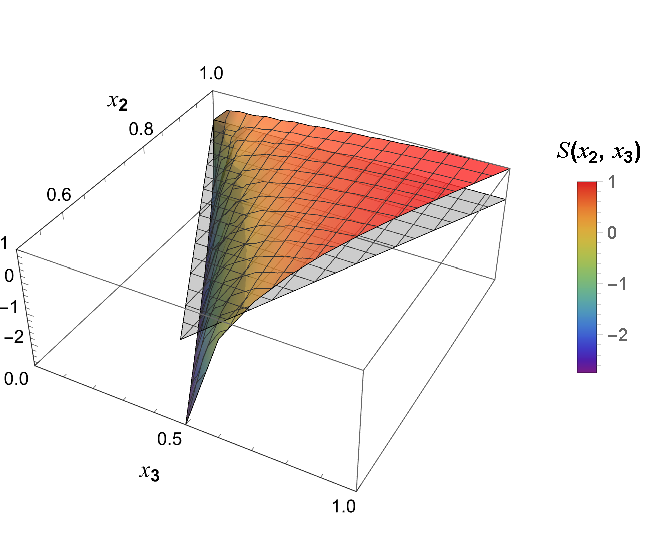
\includegraphics[width=0.4\textwidth]{figures/Shape1_low.pdf}\label{fig:cbis}}
\hfil
\sidesubfloat[]{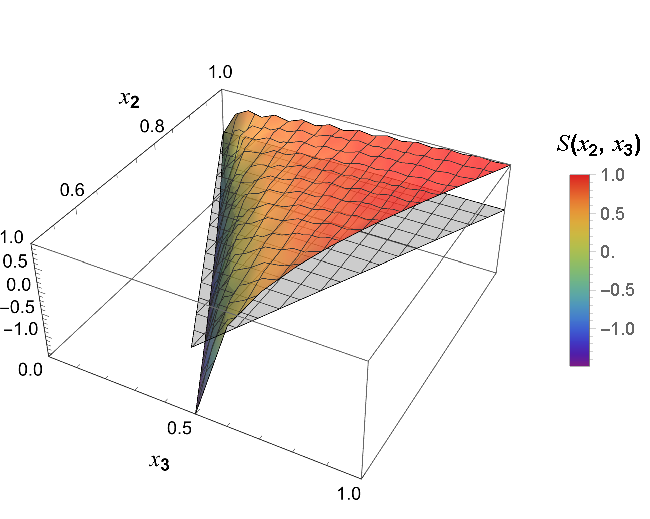
\includegraphics[width=0.4\textwidth]{figures/Shape2_low.pdf}\label{fig:dbis}}



\medskip
\sidesubfloat[]{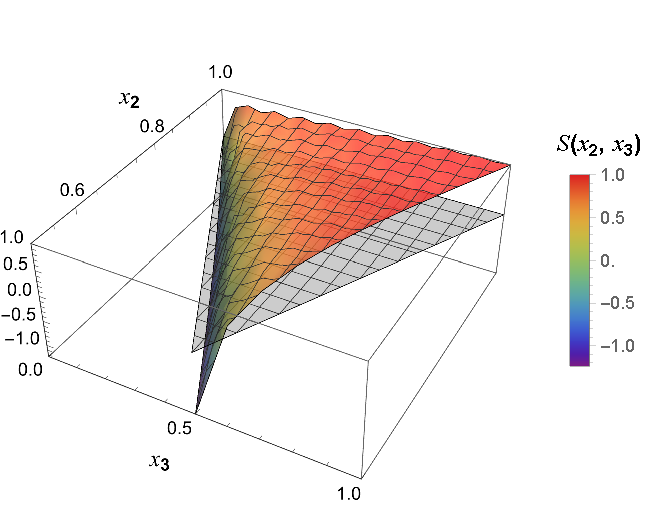
\includegraphics[width=0.4\textwidth]{figures/Shape8_low.pdf}\label{fig:ebis}}
\hfil
\sidesubfloat[]{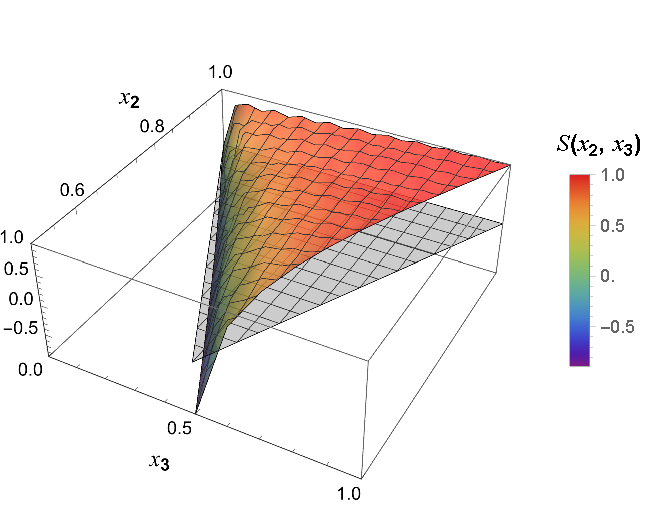
\includegraphics[width=0.4\textwidth]{figures/Shape4_low.pdf}\label{fig:fbis}}
\caption{弱い散逸$\gamma= 0.001H$の場合の、バイスペクトル形状の数値評価を示す（小さな振動は数値計算上の人工物である）。軸は外部運動量の比$  x_{2,3}:=k_{2,3}/k_{1} $である。\textbf{a.} $\left(\partial_i \pir \right)^2 \pia$演算子、\textbf{b.} $\dot{\pi}^2_{r} \pia$演算子、\textbf{c.} $\dot{\pi}_{r} \pia^2$演算子、\textbf{d.} $\pia^3$演算子。図は\cite{Salcedo:2024smn}から転載。}
\label{fig:shapes_low}
\end{figure}

    
    

\item
\(G_{aa}=0\)なので、\(a\)-\(a\)内線を含む図はすべてゼロとなる。より一般に、\(r/a\)基底は因果性を明示する。ゼロでない連結図には、それぞれの\(a\)場を図の残りに結びつけるだけの、十分な数の遅延・先進伝播子が必要である。実際、これにより、\(+\)／\(-\)基底と比べて、ゼロでない図の数が大きく減る。



\item
各頂点で運動量保存を課す。すべての頂点デルタ関数を用いると、連結相関関数に要求されるとおり、全体の因子
\begin{equation}
(2\pi)^3\delta\!\left(\sum_{a=1}^n \mathbf k_a\right)
\end{equation}
が一つ残る。



\item
図の適切な対称性因子で割る。\(+\)／\(-\)基底と同様、これにより同一の頂点と同一の内部縮約に伴う重複計数を取り除く。詳細は\cite{Goodhew:2023bcu,PajerFieldTheoryCosmologyNotes}を参照。



\item
最後に、相互作用頂点の展開から得られる伝播子への、互いに異なる、ゼロでないすべての\(r/a\)ラベル付けについて和を取る。
\end{enumerate}
ここからは、これらのFeynman規則を使い、インフレーションの開放EFTにおける原始非ガウス性を計算する。






\subsection{非ガウス性}



インフレーションの開放EFTの構築で得たすべての三次項を組み合わせ、正準基底へ再スケールすると、次の三次作用を得る。
\begin{align}\label{eq:canonormcub}
S_{\mathrm{eff}}^{(3)} =   \frac{1}{f_\pi^2} \int & \dd^4 x \Big\{\Big[4 \alpha_2 -  \frac{3}{2} (c^2_s-1) \Big]  a \pir^{\prime2} \pi'_{a} +\frac{1}{2} (c^2_s-1) a \left[\left(\partial_i \pir \right)^2 \pi'_a + 2 \pi'_{r}	\partial_i \pir  \partial^i \pia \right] \\
& \qquad \quad + \left(4 \gamma_2 - \frac{\gamma}{2}\right)  a^2\pir^{\prime2} \pia	+ \frac{\gamma}{2} a^2	\left(\partial_i \pir \right)^2 \pia \nonumber \Big. \\
&+ i \Big[\left(2\beta_7-\beta_3\right) a^2 \pi'_{r} \pi'_{a} \pia + \beta_3 a^2 \partial_i \pir  \partial^i \pia \pia + 2(\beta_4+ \beta_6 - \beta_8) a \pi'_{r} \pia^{\prime2} \Big. \nonumber \\
& \qquad \quad - 2 \beta_4  a \partial_i \pir  \partial^i \pia \pi'_{a} - 2\beta_5 a^3 \pir^{\prime} \pia^2  - 2 \beta_6 a \pir^{\prime} (\partial_i\pia)^2 \Big]  \Big. \nonumber\\
&+\delta_1 a^4 \pia^3 + (\delta_5- \delta_2) a^2 \pia^{\prime2} \pia  + \delta_2 a^2 (\partial_i \pia)^2 \pia - \delta_4 a  (\partial_i \pia)^2 \pi'_a + (\delta_4-\delta_6) a \pia^{\prime3} \Big\},  \nonumber
\end{align}


\begin{figure}[t!]
\centering
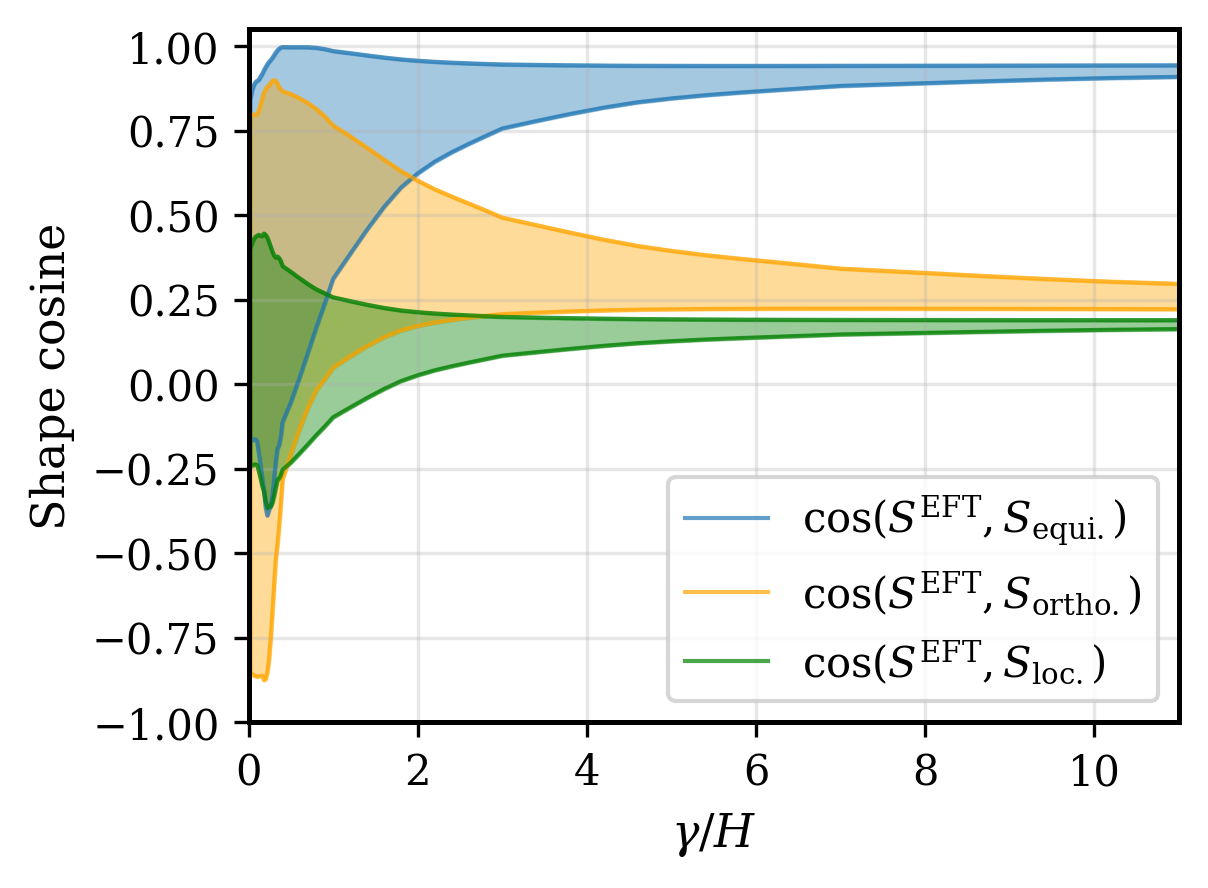
\includegraphics[width=0.6\linewidth]{figures/late_corrs.png}
\caption{Open EFToIのバイスペクトルと、\textit{Planck}の非ガウス性解析で用いられる標準的な\textit{正三角形型}、\textit{直交型}、\textit{局所型}テンプレートとの形状相関。網掛け領域は、$c_s$を$0.01$から$1$まで変化させて得られる包絡領域を示す。強散逸では、信号は$90\%$の水準で正三角形テンプレートと相関する。弱散逸では、信号は強く折り畳まれた配置でピークをもち、標準テンプレートとの相関は$c_s$に依存し、一般に直交するわけではない。図は\cite{Salcedo:2026sdn}から転載。}
\label{fig:shapecorrel}
\end{figure}



ここには明らかに、データによって制約すべき多数の新しい有効パラメータが含まれる。しかし、特に注目すべきなのは、これらの相互作用項の一部の大きさが、二次作用に現れる係数、すなわち音速$  c_{s} $と散逸$  \gamma $によって固定されることである\cite{LopezNacir:2011kk}。これらに注目すると、
\begin{align}
    S^{(3)}_{\mathrm{eff}} &= \int \dd^4 x \sqrt{-g} \bigg\{\frac{c_{s}^{2}-1}{2\fpi^{2}}\Big[\left(\partial_{i}\pir\right)^{2} \dpia +2\dpir\partial_{i}\pir\partial^{i}\pia    - 3 \dpir^{2} \dpia\Big] +\frac{\gamma}{2\fpi^{2}}\left[\left(\partial_{i}\pir\right)^{2}-\dpir^{2}\right] \pia \bigg\}\,, \nonumber
\end{align}
となる。この演算子の集合、あるいは上に書いた拡大された集合から、前小節のFeynman規則を使って木レベルのバイスペクトルを計算できる。残念ながら、解析的に計算できるのは先進場について三次の演算子だけであり、その他はすべて数値計算に頼る必要がある。代表的な数値結果を以下に示す。図\ref{fig:shapes_low}では、さまざまな三次結合についての数値結果を示す。これらの形状は、弱散逸領域で折り畳み配置に大きな信号をもつため、特に興味深い。そのため、Bunch--Davies状態でユニタリに発展するインフラトンの自己相互作用や重力相互作用から得られる非ガウス性とは、際立って異なる。この違いは、コサイン\cite{Babich:2004gb}を用いて定量化できる。正負を問わず絶対値が大きければ形状が非常によく似ていることを示し、小さければデータ上で非常に異なって見え、効果的に識別できる形状であることを意味する。最もよく研究されている、Bunch--Davies状態のユニタリな単一場スローロール・インフレーションから生じる形状とのコサインを、図\ref{fig:shapecorrel}に示す\cite{Salcedo:2026sdn}。





 

\section{確率的インフレーションとde Sitter時空の晩期の振る舞い}\label{sec:stochastic}



本節では、de Sitter空間の軽いスカラー場の長波長動力学の有効記述として、確率的インフレーションを導入する。中心的な考えは、Hubble半径程度の時間依存する粗視化尺度を使い、場を長波長モードと短波長モードに分けることである。宇宙の膨張とともにモードが絶えずこの尺度を横切るため、長波長セクターは開放系として振る舞う。その発展には、決定論的なドリフトと、粗視化したセクターへ入ってくる短波長モードが生む確率的な力の両方が含まれる。まず、質量ゼロの自由場と軽い質量をもつ自由場でこの機構を示す。これらでは、厳密なモード関数により、永年成長とその最終的な飽和が明瞭に見える。次に、対応するLangevin方程式とFokker--Planck方程式を導き、特に四次ポテンシャルに重点を置いて、相互作用する理論を調べる。これは、摂動的な永年成長、確率的再総和、非摂動的な晩期平衡分布を具体的に比較できる簡単な設定を与える。この概説は初歩的であり、最低次の確率的振る舞いだけを捉える。文献を網羅した、より詳しい議論については、例えば\cite{Woodard:2025cez,Cruces:2022imf,Vennin:2020kng}を参照されたい。ここで採る開放系の視点と、私自身がこの主題に入門したことは、C.~P.~Burgess、R.~Holmanとその共同研究者に特に多くを負っている。彼らの研究は、インフレーションのデコヒーレンスと確率的インフレーションを、マスター方程式、開放有効場理論、晩期の再総和へと結びつけた\cite{Burgess:2006jn,Burgess:2014eoa,Burgess:2015ajz}。





\subsection{系と環境の時間依存する分割}
\label{sec:stochastic-secular-growth}



固定された厳密なde Sitter背景上を伝播する、軽い傍観的スカラー場を考える。この場はエネルギー運動量テンソルに無視できない寄与をしないと仮定し、したがって幾何に影響を与えない。空間的に平坦な座標では、
\begin{equation}
ds^{2}
=
-dt^{2}
+
a^{2}(t)\,d\mathbf{x}^{2},
\qquad
a(t)
=
e^{Ht},
\end{equation}
となり、Hubbleパラメータ\(H\)は一定である。スカラー場の作用は
\begin{equation}
S
=
-\int d^{4}x\,\sqrt{-g}
\left[
\frac{1}{2}
g^{\mu\nu}
\partial_{\mu}\phi
\partial_{\nu}\phi
+
V(\phi)
\right].
\end{equation}
である。最終的には四次ポテンシャル
\begin{equation}
V(\phi)
=
\frac{\lambda}{4!}\phi^{4},
\end{equation}
に関心があるが、まず質量ゼロの自由理論を、次に小さな質量をもつ自由場を考えると有用である。後者は、永年項の起源と解釈を特に明瞭に見られる、厳密に解ける例となる。



このHamilton的な場の量子論を開放系の問題にするには、系と環境を分ける必要がある。本ノートではこれまで、系と環境の相互作用によって現れる開放系効果だけを考えてきた。しかし、開放系の動力学が現れる、概念的に異なる方法がある。鍵となる考えは、系と環境の分割を時間に依存させることである。実際、これは、StarobinskyとYokoyama\cite{Starobinsky:1986fx,Starobinsky:1994bd}が当初理解した確率的インフレーションの\textit{最低次}の記述を理解するうえで、唯一重要な要素である。実際の相互作用から追加の開放系効果も生じ、膨大な文献で研究されてきた。そこが、この問題の難しく活発に議論される部分であり、本ノートでは扱わない。



場を、次のように長波長成分と短波長成分に分ける。
\begin{align}
\phi(t,\bfx)
&=
\phi_{L}(t,\bfx)
+
\phi_{S}(t,\bfx), \\
\phi_{L}(t,\mathbf{x})
&=
\int\frac{d^{3}k}{(2\pi)^{3}}\,
W\left(\frac{k}{\epsilon aH}\right)
\phi_{\mathbf{k}}(t)
e^{i\mathbf{k}\cdot\mathbf{x}},
\end{align}
ここで\(W\)は窓関数で、\(\epsilon\lesssim 1\)である。主要な赤外の振る舞いには、窓の正確な定義は重要ではない。系を長波長モード$ \phi_{L}$、環境を短波長モード$ \phi_{S}$からなるものと定義する。この分離は、窓関数の引数$ W$によって時間に依存し、おおよそ長波長モード$ k_{L}<\epsilon aH$と短波長モード$ k_{S}>\epsilon aH$を分ける。各時刻では長短モードが相互作用していなくても、宇宙が膨張してスケール因子$ a$が増えるにつれ、短波長モードが系へ流れ込むことから、開放系効果が現れる。系と環境の相互作用を無視すると、この現象は十分簡単なので、非摂動的に記述し、摂動論が与える誤解を招く結果と比較できる。本節全体で、複雑さを段階的に増した一連の例を通じ、時間依存する分割の効果を調べる。





\paragraph{質量ゼロの自由スカラー場} 最初の例として、Bunch--Davies状態の質量ゼロの自由スカラー場を考える。厳密なモード関数は
\begin{equation}
\phi_{\mathbf{k}}(\eta)
=
\frac{H}{\sqrt{2k^{3}}}
\left(
1+ik\eta
\right)
e^{-ik\eta},
\qquad
\eta
=
-\frac{1}{aH}.
\end{equation}
である。したがって、その絶対値の二乗は
\begin{equation}
\left|
\phi_{\mathbf{k}}(\eta)
\right|^{2}
=
\frac{H^{2}}{2k^{3}}
\left(
1+k^{2}\eta^{2}
\right).
\end{equation}
となる。晩期に\(k\ll aH\)となると、これは
\begin{equation}\label{Pk}
\left|
\phi_{\mathbf{k}}(t)
\right|^{2}
\simeq
\frac{H^{2}}{2k^{3}}.
\end{equation}
に近づく。系は長波長モードからなる。重要な現象、すなわち系と環境の分割の時間依存性に集中するため、人為的な深い赤外（IR）カットオフ$ k_{\rm IR}$を導入し、これより長いモードをすべて系から取り除く。このとき、同一点での分散は積分
\begin{equation}
\left\langle
\phi_{L}^{2}(t,\mathbf{x})
\right\rangle
\simeq
\int_{k_{\mathrm{IR}}}^{\epsilon a(t)H}
\frac{d^{3}k}{(2\pi)^{3}}\,
\frac{H^{2}}{2k^{3}},
\end{equation}
で与えられ、したがって
\begin{equation}
\left\langle
\phi_{L}^{2}(t,\mathbf{x})
\right\rangle
\simeq
\frac{H^{2}}{4\pi^{2}}
\ln\left(
\frac{\epsilon a(t)H}{k_{\mathrm{IR}}}
\right).
\end{equation}
となる。等価に、ある初期時刻\(t_{0}\)に対する増加量を測れば、
\begin{equation}
\left\langle
\phi_{L}^{2}(t,\mathbf{x})
\right\rangle
-
\left\langle
\phi_{L}^{2}(t_{0},\mathbf{x})
\right\rangle
\simeq
\frac{H^{3}}{4\pi^{2}}
\left(
t-t_{0}
\right)
=
\frac{H^{2}}{4\pi^{2}}N,
\label{masslessvariancelinear}
\end{equation}
となる。ここで
\begin{equation}
N
=
\ln\left(
\frac{a(t)}{a(t_{0})}
\right)
=
H(t-t_{0})
\end{equation}
は経過したe-fold数である。この結果は、時間とともに二点関数が際限なく増大することを示し、永年効果の一例となる。



\eqref{masslessvariancelinear}の増大には簡単な物理的解釈がある。各Hubble時間の間に、Fourierモードの新たな殻が分割尺度$ \epsilon a H$を横切り、環境を離れて系の一部となる。各殻は、\eqref{Pk}から取り出される特徴的な大きさ
\begin{equation}
\delta\phi_{L}
\sim
\frac{H}{2\pi}.
\end{equation}
の、ほぼ独立した揺らぎを与える。したがって、\(N\)e-fold後には、系の長波長場$ \phi_{L}$は、およそ\(N\)回の独立したキックを受けている。通常のランダムウォークと同様、平均変位は\(
\left\langle
\phi_{L}
\right\rangle
=
0,
\)とゼロのままであり、分散はステップ数に比例して増大する。
\begin{equation}
\left\langle
\phi_{L}^{2}
\right\rangle
\sim
N
\left(
\frac{H}{2\pi}
\right)^{2}.
\end{equation}
これは\eqref{masslessvariancelinear}を再現する。したがって、長波長スカラー場は場の空間で拡散する。この質量ゼロの自由理論では、分散の線形成長は厳密な非摂動的結果である。それは、長波長セクターに独立なモードが絶えず蓄積することを反映する。一様背景上の自由理論なので、この効果は、長波長（系）モードと短波長（環境）モードの間に瞬間的な相互作用が全くなくても生じることを、再度強調しておく。





\subsection{軽い質量をもつスカラー場}
\label{sec:light-massive-scalar}



次に、小さな正の質量をもつ自由スカラー場を考える。
\begin{equation}
V(\phi)
=
\frac{1}{2}m^{2}\phi^{2},
\qquad
0<m^{2}\ll H^{2}.
\end{equation}
この理論も自由理論であるため、後期の振る舞いを厳密に決定し、摂動的な取り扱いと比較できる、とりわけ簡単な例を与える。後でこれは、それ自体では正則な結果を摂動展開したときに永年項がどのように現れるかを理解するための有用なトイモデルとなる。



共形時間を用い、\( -\infty<\eta<0\)に対して\(
\eta
=
-1/(aH)\)とする。場を次のように展開すると、
\begin{equation}
\phi(\eta,\mathbf{x})
=
\int\frac{d^{3}k}{(2\pi)^{3}}
\left[
a_{\mathbf{k}}
\phi_{k}(\eta)
e^{i\mathbf{k}\cdot\mathbf{x}}
+
a_{\mathbf{k}}^{\dagger}
\phi_{k}^{*}(\eta)
e^{-i\mathbf{k}\cdot\mathbf{x}}
\right],
\end{equation}
モード関数は次式に従う。
\begin{equation}
\phi_{k}''
-
\frac{2}{\eta}\phi_{k}'
+
\left(
k^{2}
+
\frac{m^{2}}{H^{2}\eta^{2}}
\right)
\phi_{k}
=
0.
\end{equation}
Bunch--Davies解は
\begin{equation}
\phi_{k}(\eta)
=
\frac{\sqrt{\pi}}{2}
e^{i\frac{\pi}{2}\left(\nu+\frac{1}{2}\right)}
H(-\eta)^{3/2}
H_{\nu}^{(1)}(-k\eta),
\qquad
\nu
=
\sqrt{
\frac{9}{4}
-
\frac{m^{2}}{H^{2}}
}.
\label{massiveBDmode}
\end{equation}
位相は、\(-k\eta\gg1\)となる初期時刻に、正準規格化された場が正振動数のMinkowskiモードに近づくように選んである。



軽いスカラー場に対しては、次を導入すると便利である。
\begin{equation}
\Delta
\equiv
\frac{3}{2}
-
\nu.
\end{equation}
\(m^{2}\ll H^{2}\)のとき、
\begin{equation}
\Delta
=
\frac{m^{2}}{3H^{2}}
+
\mathcal{O}\left(
\frac{m^{4}}{H^{4}}
\right).
\label{lightmassDelta}
\end{equation}
Hankel関数の引数が小さいときの振る舞いを用いると、Hubbleスケールを超えるモード関数は
\begin{equation}
\phi_{k}(\eta)
\simeq
-i\,
\frac{2^{\nu-1}\Gamma(\nu)}{\sqrt{\pi}}\,
\frac{H}{k^{3/2}}
\left(
\frac{k}{aH}
\right)^{\Delta},
\qquad
k\ll aH.
\end{equation}
したがって、その絶対値は
\begin{equation}
\left|
\phi_{k}(\eta)
\right|^{2}
\simeq
\frac{H^{2}}{2k^{3}}
\mathcal{C}(\nu)
\left(
\frac{k}{aH}
\right)^{2\Delta},
\label{massivesuperhorizonmode}
\end{equation}
ここで、
\begin{equation}
\mathcal{C}(\nu)
=
\frac{2^{2\nu-1}\Gamma^{2}(\nu)}{\pi}\overset{m\to0}{\longrightarrow} 1\,.
\end{equation}
以下では、主要な赤外の振る舞いを残し、\(\mathcal{C}(\nu)\simeq1\)とする。



質量ゼロの場合との重要な違いは、次の因子である。
\begin{equation}
\left(
\frac{k}{aH}
\right)^{2\Delta}.
\end{equation}
後期には、モード$ k$の振幅はもはや一定ではなく、$ a^{-\Delta}$としてゆっくり減衰する。したがって質量があると、我々の系に含まれる長波長モードの寄与は、時間とともに次第に小さくなる。これから見るように、これが復元力をもたらし、後期の振る舞いを有限にする。



系と環境の分割を再び考えよう。今回も\(
k_{\rm IR}
<
k
<
\epsilon a(t)H,
\)を満たす場のモードを系とし、\(k_{\rm IR}\)を固定された赤外カットオフ、\(\epsilon\lesssim1\)とする。\eqref{massivesuperhorizonmode}を用いると、系に含まれるモードの分散は
\begin{align}
\left\langle
\phi_{L}^{2}(t,\mathbf{x})
\right\rangle
&\simeq
\int_{k_{\rm IR}}^{\epsilon aH}
\frac{d^{3}k}{(2\pi)^{3}}\,
\frac{H^{2}}{2k^{3}}
\left(
\frac{k}{aH}
\right)^{2\Delta}=
\frac{H^{2}}{4\pi^{2}}
\int_{k_{\rm IR}}^{\epsilon aH}
\frac{dk}{k}
\left(
\frac{k}{aH}
\right)^{2\Delta}\\
&=
\frac{H^{2}}{8\pi^{2}\Delta}
\left[
\epsilon^{2\Delta}
-
\left(
\frac{k_{\rm IR}}{a(t)H}
\right)^{2\Delta}
\right]=\frac{H^{2}\epsilon^{2\Delta}}{8\pi^{2}\Delta}
\left[
1
-
e^{-2 N\Delta}
\right]
\label{massivevariancecutoff}
\end{align}
最後の段階では、十分早い時刻$ t_{0}$に対して\( k_{\rm IR}
=
\epsilon a(t_{0})H \)と選んだ。軽い質量の極限の主要次数では\(\epsilon^{2\Delta}\simeq 1\)と近似でき、次を得る。
\begin{equation}
\left\langle
\phi_{L}^{2}(t,\mathbf{x})
\right\rangle
\simeq
\frac{H^{2}}{8\pi^{2}\Delta}
\left[
1
-
e^{-2N\Delta }
\right].
\label{exactmassivevariance}
\end{equation}
\eqref{lightmassDelta}を用いれば、これは同値に次のようにも書ける。
\begin{equation}
\left\langle
\phi_{L}^{2}(t,\mathbf{x})
\right\rangle
\simeq
\frac{3H^{4}}{8\pi^{2}m^{2}}
\left[
1
-
\exp\left(
-\frac{2m^{2}}{3H}(t-t_{0})
\right)
\right].
\label{exactlightmassivevariance}
\end{equation}
鋭い窓関数に対してHubbleスケールを超える領域で成り立つこの非摂動的な結果は、質量ゼロの自由スカラー場で現れた後期の発散\eqref{masslessvariancelinear}が、小さいながらも有限の質量がある場合には存在しないことを示している。直観的には、各時間ステップで短波長の環境から長波長の系へ新しいモードが入ることによる広がりが、二次ポテンシャルの復元力と釣り合うのである。





\paragraph{摂動展開と永年成長} 次に、上の非摂動的な結果を、質量項を摂動的に扱ったなら得られる結果と比較する。最も簡単な方法は、非摂動的な結果を\(\Delta\)のべき、あるいは同値に\(m^{2}/H^{2}\)のべきで展開することである。見通しを得るため、これは$m = 0 $のまわりの展開であり、その場合には先ほど見たように後期に実際の発散があることに注意しよう。このことは、摂動論にもこれらの永年発散が現れるだろうと警告している。



\eqref{exactmassivevariance}を展開すると、次を得る。
\begin{align}
\left\langle
\phi_{L}^{2}(t,\mathbf{x})
\right\rangle
&=
\frac{H^{2}}{4\pi^{2}}
\left[
N
-
 N^{2}\Delta
+
\frac{2}{3}N^{3}\Delta^{2}
+
\cdots
\right]
\label{perturbativemassivevariance}\\
&\simeq 
\frac{H^{2}}{4\pi^{2}}
\left[
N
-
\frac{m^{2}}{3H^{2}}N^{2}
+
\frac{2m^{4}}{27H^{4}}N^{3}
+
\cdots
\right],
\end{align}
ここで\(\Delta\simeq m^{2}/(3H^{2})\)を用いた。\(
N\Delta 
\ll
1
\)となる初期には、この展開は非摂動的な結果と一致する。しかし後期には、\(N\)の永年的なべきが質量の小ささを補い、次の条件で摂動論が破綻する。
\begin{equation}
N\Delta 
\sim
1,
\qquad\text{または同値に}\qquad
N
\sim
\frac{H^{2}}{m^{2}}.
\end{equation}
したがって、最初から摂動的に計算したなら、質量ゼロの結果に対する補正が際限なく大きくなると予測するように見える。



非摂動解は、この見かけの破綻が物理的不安定性ではなく、摂動論に起因する人工的なものであることを示している。完全な分散\eqref{exactlightmassivevariance}は有限にとどまり、次の値に近づく。
\begin{equation}
\lim_{t\rightarrow\infty}
\left\langle
\phi_{L}^{2}(t,\mathbf{x})
\right\rangle
=
\frac{H^{2}}{8\pi^{2}\Delta}
\simeq
\frac{3H^{4}}{8\pi^{2}m^{2}}.
\end{equation}
永年項は、因子\(
e^{-2\Delta N}
\)を\(\Delta\)のべきで展開することから生じる。この指数関数を展開せずに保てば、\(N\Delta \)のべきで増強された項の級数全体が再総和され、後期の正しい正則な振る舞いが回復する。これは、永年成長が理論そのものの性質ではなく、厳密な摂動展開に起因する人工的なものである典型例を与える。\\



これまでのde Sitter時空における軽い場の議論は、Hilbert空間の分割という点で開放系と関係していたが、本講義で展開した手法は用いていなかった。それは、これまで調べたのが、非摂動解を容易に得られる三つの理論だけだったためである。



ここからは、完全な解が知られていない相互作用する理論へ進む。そのために、系と環境の時間依存する分割の効果を総和する手法を構築する。前述のように、系と環境の間の瞬間的な相互作用は主要次数に寄与しないので、すべて実質的に無視する。





\subsection{長波長場に対するLangevin方程式}
\label{sec:stochastic-langevin}



次に、質量ゼロの相互作用する理論を考える。
\begin{equation}
V(\phi)
=
\frac{\lambda}{4!}\phi^{4},
\qquad
\lambda>0.
\end{equation}
質量をもつ例と同様、厳密な摂動展開は、経過したe-fold数とともに永年的に成長する項を生む。例えば、同一点の二点関数における主要な赤外項は\cite{Cespedes:2023aal}
\begin{align}
\left\langle
\phi_{L}^{2}
\right\rangle
&=
\frac{H^{2}}{4\pi^{2}}
\left[
N
-
\frac{\lambda}{36\pi^{2}}N^{3}
+
\frac{\lambda^{2}}{720\pi^{4}}N^{5}
-
\frac{53\lambda^{3}}{544320\pi^{6}}N^{7}
+
\cdots
\right].
\label{quarticsecularseries}
\end{align}
第1項はツリーレベル、第2項は1ループであり、以下も同様である。より一般には、
\begin{equation}
\left\langle
\phi_{L}^{2}
\right\rangle_{n\text{ループ}}
\sim
H^{2}\lambda^{n}N^{2n+1}.
\end{equation}
したがって有効な展開パラメータは\(\lambda N^{2}\)であり、\(N\sim\lambda^{-1/2}\)になると摂動論は信頼できなくなる。時間発展を時間について摂動展開せずに、これらの主要な赤外効果を捉える発展方程式を導こう。





\paragraph{位相空間での粗視化}



系統的な導出では、粗視化した場とその速度の両方を位相空間変数として保持する\cite{Grain:2017dqa,Vennin:2020kng}。近年の開放系による定式化については\cite{Christie:2026qsi}も参照されたい。確率的近似の主要次数では、粗視化スケールを横切る短波長モードは、自由なBunch--Daviesモード関数を用いて評価できる。次のように定義する。
\begin{align}
\phi_{L}(t,\mathbf{x})
&=
\int\frac{d^{3}k}{(2\pi)^{3}}\,
W_{t}(k)
\left[
a_{\mathbf{k}}u_{k}(t)e^{i\mathbf{k}\cdot\mathbf{x}}
+
a_{\mathbf{k}}^{\dagger}u_{k}^{*}(t)e^{-i\mathbf{k}\cdot\mathbf{x}}
\right],
\label{longfieldmovingwindow}
\\
v_{L}(t,\mathbf{x})
&=
\int\frac{d^{3}k}{(2\pi)^{3}}\,
W_{t}(k)
\left[
a_{\mathbf{k}}\dot u_{k}(t)e^{i\mathbf{k}\cdot\mathbf{x}}
+
a_{\mathbf{k}}^{\dagger}\dot u_{k}^{*}(t)e^{-i\mathbf{k}\cdot\mathbf{x}}
\right],
\end{align}
ここで、
\begin{equation}
W_{t}(k)
=
W\left(\frac{k}{k_{c}(t)}\right),
\qquad
k_{c}(t)
=
\epsilon a(t)H.
\end{equation}
窓関数が時間に依存するため、\(v_{L}\)は\(\dot\phi_{L}\)と等しくない。微視的なHeisenberg場は次式に従う。
\begin{equation}
\ddot{\phi}(t,\mathbf{x})
+
3H\dot{\phi}(t,\mathbf{x})
-
\frac{1}{a^{2}(t)}
\nabla^{2}\phi(t,\mathbf{x})
+
V'\!\left(\phi(t,\mathbf{x})\right)
=
0.
\label{microscopic_field_equation}
\end{equation}
二つの定義を微分して微視的な場の方程式を用いると、空間勾配および瞬間的な長波長・短波長間相互作用の主要なゼロ次において、次を得る。
\begin{align}
\dot\phi_{L}
&=
v_{L}
+
\hat\xi_{\phi},
\label{phase_space_langevin_phi}
\\
\dot v_{L}
&=
-3Hv_{L}
-
V'(\phi_{L})
+
\hat\xi_{v},
\label{phase_space_langevin_v}
\end{align}
ここで二つのノイズ演算子は
\begin{align}
\hat\xi_{\phi}(t,\mathbf{x})
&=
\int\frac{d^{3}k}{(2\pi)^{3}}\,
\dot W_{t}(k)
\left[
a_{\mathbf{k}}u_{k}(t)e^{i\mathbf{k}\cdot\mathbf{x}}
+
a_{\mathbf{k}}^{\dagger}u_{k}^{*}(t)e^{-i\mathbf{k}\cdot\mathbf{x}}
\right],
\label{noiseoperator}
\\
\hat\xi_{v}(t,\mathbf{x})
&=
\int\frac{d^{3}k}{(2\pi)^{3}}\,
\dot W_{t}(k)
\left[
a_{\mathbf{k}}\dot u_{k}(t)e^{i\mathbf{k}\cdot\mathbf{x}}
+
a_{\mathbf{k}}^{\dagger}\dot u_{k}^{*}(t)e^{-i\mathbf{k}\cdot\mathbf{x}}
\right].
\label{velocitynoiseoperator}
\end{align}
したがって、ノイズは位相空間での発展の全体にわたって存在する。これは、短波長部門と長波長部門を隔てる移動する境界を、モードが横切ることから生じる。





\paragraph{ノイズ相関}



\(U_{\phi,k}=u_{k}\)および\(U_{v,k}=\dot u_{k}\)と書くと便利である。Bunch--Davies状態では、位相空間の完全なノイズ核は
\begin{equation}
\begin{aligned}
\frac{1}{2}
\left\langle
\left\{
\hat\xi_{A}(t,\mathbf{x}),
\hat\xi_{B}(t',\mathbf{x}')
\right\}
\right\rangle
&=
\operatorname{Re}
\int\frac{d^{3}k}{(2\pi)^{3}}\,
\dot W_{t}(k)\dot W_{t'}(k)
\\
&\quad\times
U_{A,k}(t)U_{B,k}^{*}(t')
e^{i\mathbf{k}\cdot(\mathbf{x}-\mathbf{x}')},
\qquad
A,B\in\{\phi,v\}.
\end{aligned}
\label{genericnoisekernel}
\end{equation}
また、\(\langle\hat\xi_{A}\rangle=0\)である。
具体的に、鋭い窓関数を考えよう。
\begin{equation}
W_{t}(k)
=
\Theta(k_{c}(t)-k),
\qquad
\dot W_{t}(k)
=
Hk_{c}(t)\delta(k-k_{c}(t)).
\end{equation}
\eqref{genericnoisekernel}に現れる二つのデルタ関数から、
\begin{equation}
\delta\left(k_{c}(t)-k_{c}(t')\right)
=
\frac{1}{Hk_{c}(t)}\delta(t-t'),
\end{equation}
したがってノイズは時間について局所的である。質量ゼロのBunch--Daviesモード関数に対しては、次を得る。
\begin{align}
\frac{1}{2}
\left\langle
\left\{
\hat\xi_{\phi}(t,\mathbf{x}),
\hat\xi_{\phi}(t',\mathbf{x}')
\right\}
\right\rangle
&=
\frac{H^{3}}{4\pi^{2}}
\left(1+\epsilon^{2}\right)
\frac{\sin\left(k_{c}(t)r\right)}{k_{c}(t)r}
\delta(t-t'),
\qquad
r=|\mathbf{x}-\mathbf{x}'|.
\label{spatialnoisecorrelator}
\end{align}
さらに、横切りのスケール\(k=\epsilon aH\)において、
\begin{equation}
\frac{\dot u_{k}}{Hu_{k}}
=
-\frac{\epsilon^{2}}{1-i\epsilon}.
\end{equation}
したがって、\(\hat\xi_{v}\)を含む相関関数は\(\epsilon^{2}\)のべきで抑制される。\(D_{AB}\)を局所的な位相空間ノイズ行列とすれば、
\begin{equation}
\frac{D_{\phi v}}{H D_{\phi\phi}}
=
\mathcal O(\epsilon^{2}),
\qquad
\frac{D_{vv}}{H^{2}D_{\phi\phi}}
=
\mathcal O(\epsilon^{4}).
\label{velocitynoisesuppression}
\end{equation}
同一点で、\(\epsilon\ll1\)に対する主要次数において、場のノイズはしたがって次式を満たす。
\begin{equation}
\left\langle
\xi_{\phi}(t,\mathbf{x})
\xi_{\phi}(t',\mathbf{x})
\right\rangle_{\xi}
=
\frac{H^{3}}{4\pi^{2}}
\delta(t-t'),
\label{classicalnoisecorrelator}
\end{equation}
ここでは、Hubbleスケールを超えるモードの古典化を用いて、演算子ノイズを古典的なガウス確率変数に置き換えた。





\paragraph{過減衰極限への縮約}



長波長の力学の適切な出発点は、式\eqref{phase_space_langevin_phi}と\eqref{phase_space_langevin_v}である。これらを一つの二階方程式にまとめると、代わりに次を得る。
\begin{equation}
\ddot\phi_{L}
+
3H\dot\phi_{L}
+
V'(\phi_{L})
=
\dot\xi_{\phi}
+
3H\xi_{\phi}
+
\xi_{v}.
\label{secondorderlangevin}
\end{equation}
鋭い窓関数では\(\xi_{\phi}\)は白色ノイズなので、\(\dot\xi_{\phi}\)を操作するよりも、位相空間で直接、過減衰極限への縮約を行う方がよい。



速度はHubble時間スケールで緩和する一方、\(|V''|\ll H^{2}\)を満たす軽い場はそれよりゆっくり変化する。\eqref{phase_space_langevin_v}から\(v_{L}\)を断熱的に消去すると、
\begin{equation}
v_{L}
\simeq
-\frac{V'(\phi_{L})}{3H}
+
\frac{\xi_{v}}{3H}.
\end{equation}
この結果を\eqref{phase_space_langevin_phi}に代入し、抑制\eqref{velocitynoisesuppression}を用いると、主要な確率的方程式を得る。
\begin{equation}
\dot{\phi}_{L}(t,\mathbf{x})
=
-\frac{V'(\phi_{L})}{3H}
+
\xi(t,\mathbf{x}),
\qquad
\xi\equiv\xi_{\phi},
\label{stochasticinflationlangevin}
\end{equation}
ここで、
\begin{equation}
\left\langle
\xi(t,\mathbf{x})
\right\rangle_{\xi}
=
0,
\qquad
\left\langle
\xi(t,\mathbf{x})
\xi(t',\mathbf{x})
\right\rangle_{\xi}
=
\frac{H^{3}}{4\pi^{2}}
\delta(t-t').
\label{stochasticinflationnoise}
\end{equation}
ドリフトはポテンシャル中のゆっくりした古典的運動を表し、ノイズは時間依存する系と環境の境界を越えてモードが絶えず加わることを表す。これが主要次数のStarobinskyのLangevin方程式である\cite{Starobinsky:1986fx,Starobinsky:1994bd}。

























































































































































































































































































































































\subsection{確率的インフレーションにおけるFokker--Planck発展}
\label{sec:stochastic-fokker-planck}



確率的近似の主要次数で、長波長場はガウス白色ノイズをもつ\eqref{stochasticinflationlangevin}のLangevin方程式に従うことを示した。以下では空間依存性を省略する。



\eqref{fokkerplanckgeneral}で導いた、加法的ノイズをもつ一階Langevin方程式と、それに対応するFokker--Planck方程式の一般的な関係を用いると、確率密度\(P(\phi,t)\)は次式に従う。
\begin{equation}
\frac{\partial P(\phi,t)}{\partial t}
=
\frac{1}{3H}
\frac{\partial}{\partial\phi}
\left[
V'(\phi)P(\phi,t)
\right]
+
\frac{H^{3}}{8\pi^{2}}
\frac{\partial^{2}P(\phi,t)}{\partial\phi^{2}}.
\label{stochasticinflationFP}
\end{equation}
第1項はポテンシャルが生む決定論的なドリフトを表し、第2項は長波長部門に絶えず入ってくるモードによる場の空間での拡散を表す。



直観を得るため、\eqref{stochasticinflationFP}を連続の式として書くことができる。このとき確率流は
\begin{equation}
J(\phi,t)
=
-
\frac{V'(\phi)}{3H}
P(\phi,t)
-
\frac{H^{3}}{8\pi^{2}}
\frac{\partial P(\phi,t)}{\partial\phi}.
\label{FPcurrent}
\end{equation}
第1の寄与は古典的なスローロールの流れに沿って確率を運び、第2の寄与は確率密度の高い領域から低い領域へ確率を運ぶ。



式\eqref{stochasticinflationFP}は、時間について一階の発展方程式である。
\begin{equation}
\frac{\partial P}{\partial t}
=
\mathcal{L}_{\rm FP}P,
\end{equation}
ここでFokker--Planck生成子は
\begin{equation}\label{FPeq}
\mathcal{L}_{\rm FP}
=
\frac{1}{3H}
\frac{\partial}{\partial\phi}
V'(\phi)
+
\frac{H^{3}}{8\pi^{2}}
\frac{\partial^{2}}{\partial\phi^{2}},
\end{equation}
第1項は積\(V'(\phi)P\)に作用するものと理解する。この生成子が得られれば、解を時間について摂動展開することなく、その時間発展を解ける。これこそがStarobinskyの重要な洞察であり、摂動論で現れる永年効果の本当の性質を理解することを可能にする。\eqref{FPeq}と第\ref{ssec:resummation}節の議論との類似性に注意されたい。これは量子マスター方程式の確率的な対応物とみなせる。





\paragraph{自由場}



最初の確認として、質量ゼロの自由理論\(
V(\phi)
=
0.
\)を考える。
Fokker--Planck方程式は通常の拡散方程式に帰着する。
\begin{equation}
\frac{\partial P}{\partial t}
=
\frac{H^{3}}{8\pi^{2}}
\frac{\partial^{2}P}{\partial\phi^{2}}.
\label{masslessdiffusionequation}
\end{equation}
鋭く局在した初期条件
\begin{equation}
P(\phi,t_{0})
=
\delta(\phi-\phi_{0}),
\end{equation}
に対する解は次である。\footnote{注意深い読者は、\eqref{masslessdiffusionequation}がSchr\"odinger方程式のWick回転であり、この解が量子調和振動子の基底状態であると気づくだろう。}
\begin{equation}
P(\phi,t)
=
\frac{1}{
\sqrt{
4\pi D(t-t_{0})
}
}
\exp\left[
-
\frac{
(\phi-\phi_{0})^{2}
}{
4D(t-t_{0})
}
\right],
\qquad
D
=
\frac{H^{3}}{8\pi^{2}}.
\label{masslessGaussianP}
\end{equation}
平均は一定にとどまり、
\begin{equation}
\left\langle
\phi
\right\rangle
=
\phi_{0},
\end{equation}
一方、分散は次のように増大する。
\begin{equation}
\left\langle
(\phi-\phi_{0})^{2}
\right\rangle
=
2D(t-t_{0})
=
\frac{H^{3}}{4\pi^{2}}
(t-t_{0}).
\label{masslessFPvariance}
\end{equation}
\(\phi_{0}=0\)に対して、これは\eqref{masslessvariancelinear}で非摂動的なモード関数から直接得た永年成長を再現する。したがってFokker--Planck方程式は、質量ゼロの自由場のランダムウォークという解釈を再現する。



次に、二次ポテンシャルをもつ質量のある自由場を考える。
\begin{equation}
V(\phi)
=
\frac{1}{2}m^{2}\phi^{2}.
\end{equation}
式\eqref{stochasticinflationFP}は次のようになる。
\begin{equation}
\frac{\partial P}{\partial t}
=
\frac{m^{2}}{3H}
\frac{\partial}{\partial\phi}
\left[
\phi P
\right]
+
\frac{H^{3}}{8\pi^{2}}
\frac{\partial^{2}P}{\partial\phi^{2}}.
\label{massiveOrnsteinUhlenbeck}
\end{equation}
これはOrnstein--Uhlenbeck過程のFokker--Planck方程式である。



確率分布全体を解く代わりに、二次モーメントの発展を直接導くこともできる。\eqref{massiveOrnsteinUhlenbeck}に\(\phi^{2}\)を掛け、\(\phi\)について積分し、境界項が消えると仮定すると、次を得る。
\begin{equation}
\frac{d}{dt}
\left\langle
\phi^{2}
\right\rangle
=
-
\frac{2m^{2}}{3H}
\left\langle
\phi^{2}
\right\rangle
+
\frac{H^{3}}{4\pi^{2}}.
\label{massivesecondmomentequation}
\end{equation}
初期条件
\begin{equation}
\left\langle
\phi^{2}(t_{0})
\right\rangle
=
0,
\end{equation}
に対する解は
\begin{equation}
\left\langle
\phi^{2}(t)
\right\rangle
=
\frac{3H^{4}}{8\pi^{2}m^{2}}
\left[
1
-
\exp\left(
-\frac{2m^{2}}{3H}
(t-t_{0})
\right)
\right].
\label{massiveFPvariance}
\end{equation}
これは\eqref{exactlightmassivevariance}で質量のある厳密なモード関数から直接得た結果と一致する。したがって確率的記述は、質量ゼロの場の際限のない拡散と、軽い質量をもつ場の後期の有限な分散の両方を再現する。Fokker--Planck方程式の優れた点は、時間依存する系と環境の分割の効果を再総和するこの能力を、相互作用する理論へ拡張できることである。





\paragraph{定常分布}



一般のポテンシャル\(V(\phi)\)に戻ろう。定常解は
\begin{equation}
\frac{\partial P_{\rm eq}}{\partial t}
=-\frac{\partial J_{\rm eq}}{\partial \phi} =0,
\end{equation}
を満たすので、その確率流は\(\phi\)によらない。実数直線全体で規格化可能な平衡分布では、流れはゼロでなければならず、\(
J_{\rm eq}(\phi)
=
0.
\)である。
\eqref{FPcurrent}を用いると、この条件は
\begin{equation}
\frac{H^{3}}{8\pi^{2}}
\frac{dP_{\rm eq}}{d\phi}
=
-
\frac{V'(\phi)}{3H}
P_{\rm eq}(\phi).
\end{equation}
これを解くと、
\begin{equation}
P_{\rm eq}(\phi)
=
\frac{1}{Z}
\exp\left[
-
\frac{8\pi^{2}}{3H^{4}}
V(\phi)
\right],
\label{StarobinskyYokoyamaDistribution}
\end{equation}
ここで、
\begin{equation}
Z
=
\int_{-\infty}^{+\infty}
d\phi\,
\exp\left[
-
\frac{8\pi^{2}}{3H^{4}}
V(\phi)
\right]
\end{equation}
は規格化によって定まる。



定常確率分布が存在するのは、この積分が収束する場合に限られる。したがって質量ゼロの自由理論には、規格化可能な平衡分布は存在せず、これはその際限のない拡散と整合する。これに対し、\(\lvert\phi\rvert\rightarrow\infty\)で十分速く増大するポテンシャルは、いずれも規格化可能な定常分布をもつ。このような場合、ポテンシャルの低い値に向かう決定論的なドリフトは、長波長部門に入るモードが引き起こす絶え間ない拡散と、最終的に釣り合う。




 

\subsection{四次ポテンシャル}



ここで四次ポテンシャルに注目しよう。
\begin{equation}
V(\phi)
=
\frac{\lambda}{4!}\phi^{4}.
\end{equation}
この場合、Fokker--Planck方程式は二つの相補的な領域で解ける。初期には$ \lambda N^{2}$の展開として、非常に遅い時刻には先ほど求めた平衡分布のまわりで解く。





\paragraph{摂動解} Fokker--Planck方程式\eqref{stochasticinflationFP}は、確率分布のモーメントに対する連立した方程式の階層を与える。\eqref{stochasticinflationFP}に\(\phi^{n}\)を掛け、\(\phi\)について積分し、境界項が消えると仮定すると、次を得る。
\begin{equation}\label{quarticmomenthierarchy}
\frac{d}{dN}
\left\langle
\phi^{n}
\right\rangle
=
-
\frac{n\lambda}{18H^{2}}
\left\langle
\phi^{n+2}
\right\rangle
+
\frac{n(n-1)H^{2}}{8\pi^{2}}
\left\langle
\phi^{n-2}
\right\rangle ,
\end{equation}
ここでは時間変数をe-fold数\(N=H(t-t_{0})\)に切り替えた。この方程式は閉じていない。二点関数は四点関数に依存し、その発展はさらに六点関数に依存する、という具合である。それでも、この階層は\(\lambda\)の展開として再帰的に解ける。



初めに\(\phi=0\)に局在した分布に対し、質量ゼロの自由理論では
\begin{equation}
\left\langle
\phi^{2n}
\right\rangle_{0}
=
(2n-1)!!
\left(
\frac{H^{2}N}{4\pi^{2}}
\right)^{n},
\qquad
\left\langle
\phi^{2n+1}
\right\rangle_{0}
=
0.
\end{equation}
これらのモーメントを$ n=2$の場合の\eqref{quarticmomenthierarchy}に代入すると最初の摂動補正が得られ、この手続きを次数ごとに繰り返せる。二点関数について、得られる展開は次の形をとる。
\begin{equation}
\left\langle
\phi^{2}(N)
\right\rangle
=
H^{2}
\sum_{p=0}^{\infty}
c_{p}\lambda^{p}N^{2p+1},
\label{quarticperturbativeseries}
\end{equation}
係数\(c_{p}\)はモーメントの階層によって再帰的に決定される。最初の数項は
\begin{equation}
\left\langle
\phi^{2}(N)
\right\rangle
=
\frac{H^{2}}{4\pi^{2}}
\left[
N
-
\frac{\lambda}{36\pi^{2}}N^{3}
+
\mathcal O\left(
\lambda^{2}N^{5}
\right)
\right].
\label{quarticfirstsecularterms}
\end{equation}


これらの項は、摂動的な場の量子論で得られる主要な赤外の永年寄与を再現する。より一般には、確率的な階層は\(\lambda^{p}\)次において、次に比例する主要な寄与を生む。
\begin{equation}
\lambda^{p}N^{2p+1}.
\end{equation}
予想したように、摂動展開を制御するのは\(\lambda\)だけではなく、組合せ\(
\lambda N^{2},
\)である。結合がどれほど小さくても、\(
N
\sim \lambda^{-1/2}
\)になると厳密な摂動展開はやがて破綻する。





\paragraph{非摂動的な平衡解}



モーメント展開は、\(\lambda\)の固定次数でFokker--Planck方程式の初期の解を記述するが、後期には破綻する。定常分布の非摂動的な導出から、これらの永年効果は摂動論に起因する人工的なものかもしれないと、すでに推測できる。したがって後期の振る舞いを決めるため、代わりに定常分布\eqref{StarobinskyYokoyamaDistribution}を調べる。四次ポテンシャルに対しては、
\begin{equation}
P_{\rm eq}(\phi)
=
\frac{1}{Z}
\exp\left[
-
\frac{\pi^{2}\lambda}{9H^{4}}
\phi^{4}
\right],
\label{quarticequilibriumdistribution}
\end{equation}
これは\(\lambda>0\)で規格化可能であり、四次相互作用が質量ゼロの自由場の際限のない拡散を食い止めることを示している。



これで、長波長場のすべての等時刻モーメントを、\(\lambda\)について展開せずに評価できる。平衡分布は偶関数なので、すべての奇数次モーメントは消える。
\begin{equation}
\left\langle
\phi^{2n+1}
\right\rangle_{\rm eq}
=
0.
\end{equation}
偶数次モーメントは
\begin{equation}
\left\langle
\phi^{2n}
\right\rangle_{\rm eq}
=
\left( \frac{\pi^{2}\lambda}{9H^{4}} \right)^{-n/2}
\frac{
\Gamma\left(
\frac{2n+1}{4}
\right)
}{
\Gamma\left(
\frac{1}{4}
\right)
}.
\label{quarticequilibriummoments}
\end{equation}
特に、
\begin{equation}
\left\langle
\phi^{2}
\right\rangle_{\rm eq}
=
\frac{3H^{2}}{\pi\sqrt{\lambda}}
\frac{
\Gamma\left(
\frac{3}{4}
\right)
}{
\Gamma\left(
\frac{1}{4}
\right)
},
\label{quarticequilibriumtwopoint} \qquad 
\left\langle
\phi^{4}
\right\rangle_{\rm eq}
=
\frac{9H^{4}}{4\pi^{2}\lambda}.
\end{equation}


平衡における二点関数は有限だが、結合について非解析的である。したがって、摂動論のいかなる有限次数でも再現できない。これはむしろ、モーメントの階層が生む永年項の級数全体を再総和した結果を表している。



摂動的記述と平衡での記述の関係は、次元解析によって明確にできる。時間に依存する完全な解は、次のスケーリング形式をとらなければならない。
\begin{equation}
\left\langle
\phi^{2}(N)
\right\rangle
=
\frac{H^{2}}{\sqrt{\lambda}}\,
F\left(
\sqrt{\lambda}\,N
\right),
\label{quarticscalingform}
\end{equation}
ここで\(F\)はある無次元関数である。初期の\(\sqrt{\lambda}\,N\ll1\)では、摂動的な階層がそのTaylor展開を定める。
\begin{equation}
F(z)
=
\frac{z}{4\pi^{2}}
-
\frac{z^{3}}{144\pi^{4}}
+
\cdots.
\end{equation}
後期には、平衡分布がその漸近値を定める。
\begin{equation}
F(z)
\xrightarrow{z\rightarrow\infty}
\frac{3}{\pi}
\frac{
\Gamma\left(
\frac{3}{4}
\right)
}{
\Gamma\left(
\frac{1}{4}
\right)
}.
\end{equation}
完全なFokker--Planck発展は、この二つの領域をつなぐ補間を与える。平衡分布の近傍での時間発展は、Fokker--Planck生成子の固有ベクトルを通じて調べられるが、ここではこの議論を省略する。関心のある読者は文献を参照されたい。





\section{結論と展望}




本講義では、開放量子系に対する二つの相補的な記述を展開した。演算子形式では、密度行列、部分トレース、完全正値な力学写像から出発し、Markov性と時間一様性の仮定のもとで、Gorini--Kossakowski--Sudarshan--Lindbladマスター方程式と、そのHamiltonianによる寄与および散逸的な寄与に到達した。



続いてSchwinger--Keldysh経路積分を導入した。二重化された場は時間順序積と反時間順序積を符号化し、\(r/a\)基底は応答と揺らぎを分離する。環境を積分消去すると、散逸、ノイズ、デコヒーレンスを記述するFeynman--Vernon影響汎関数が得られる。その二次の半古典極限はしばしばLangevin記述を許すが、完全な有効作用には、ガウス型の確率的力学を超える、本質的に量子的な相互作用が含まれうる。



これらの考え方をインフレーションに適用し、破れた時間並進に対応するGoldstoneボソンの開放有効場理論を構築した。この枠組みは環境による散逸と揺らぎを系統的に取り込み、純粋に古典的な確率的対応物をもたない相互作用も含めて、パワースペクトルと原始非ガウス性の計算に用いることができる。



最後に、de Sitter時空における長波長モードと短波長モードの時間依存する分割から、軽い場の確率的発展が導かれた。相互作用する場では、得られるFokker--Planck方程式が、時間とともに永年的に成長する摂動的寄与を再総和し、後期に正則な分布へ近づくことがある。このような永年成長は、必ずしも物理的不安定性を意味しない。むしろ、発展方程式を摂動論の有効範囲を超えて展開したことを示している場合がある。



\paragraph{演算子と経路積分の視点。}



演算子形式と経路積分形式を併せて提示した動機の一つは、それぞれが、他方では比較的見えにくい構造を明らかにすることである。密度行列の言語は、状態、エントロピー、量子チャネル、完全正値性に関する問題に特に適している。一方、Schwinger--Keldyshの言語は、局所性、対称性、有効場理論、および一般の多時刻相関関数の計算に自然に適している。原理的には、二つの記述は同じ物理を符号化しているが、関連する情報の整理の仕方は大きく異なる。



本講義のいくつかの例は、二つの視点を組み合わせることで何が学べるかを示している。生成汎関数の規格化や有効作用の虚部の正値性といった基本的なSchwinger--Keldysh条件だけでも、影響汎関数に重要な制限が課される。それでも、時間について局所的な影響汎関数がGKSL生成子で記述できる場合、完全正値性はさらに強い制約を課す。上で調べたガウス型の例では、Kossakowski行列の正値性が散逸係数とノイズ係数を関連づけ、ゼロでない摩擦には、それに伴う揺らぎの最低限の量が必要であることを示す。より一般には、影響汎関数を直接展開する代わりにジャンプ演算子を展開することで、打ち切り後も完全正値性が厳密に保たれうる、正値性を改善した有効理論を構成する方法が得られる。



逆に、Schwinger--Keldysh形式は、密度行列を時間発展させて等時刻期待値を評価することで最も直接的に得られるものよりも、はるかに広い種類の観測量を自然に生成する。二重化された源に関する汎関数微分は異なる時間順序をもつ相関関数を生み、$r/a$基底は応答関数と揺らぎの関数を効率よく整理する。主要な観測量が密度行列そのものではなく量子場の相関関数である宇宙論では、これは特に有用である。演算子形式は許容される発展に強力な構造的制約を与え、経路積分はそれらの制約を時空対称性や有効場理論と組み合わせるための言語を提供する。



ここで扱った応用は、ほぼすべて初期宇宙、より具体的にはインフレーションに限られている。したがって、これらは、開放系の手法が宇宙論で果たしうる、はるかに広い役割の最初の例示とみなすべきである。宇宙論の多くの問題では、観測されるのは限られた範囲のスケール、粒子種、あるいは集団変数だけであり、残りの自由度は環境として働く。そのとき粗視化は、一般に散逸項、揺らぎ、記憶効果を生み、保持された変数に制限した発展はユニタリであるとは限らない。



よく研究されている例として、大規模構造の有効場理論がある。長波長の物質分布の有効記述を得るため、短波長の非線形モードを積分消去する。その結果には有効応力と確率的寄与が含まれるため、この意味で開放統計理論である。従来は運動方程式とその相関関数によって直接定式化されてきたが、同値な経路積分形式を用いれば、対称性、応答場、確率的項、くりこみの性質を統一的に整理できるはずである。



宇宙論と宇宙素粒子物理には、さらに多くの応用の可能性がある。宇宙の熱的歴史には、再加熱、熱化、粒子生成、凍結をはじめ、進化する媒質と相互作用する部分系の例が繰り返し現れる。ニュートリノ振動と輸送、暗黒物質の運動論、バリオン数生成、物質中の重力波の伝播、追加の部門が存在する場合の宇宙論的摂動の発展は、いずれも適切な領域では開放系による記述の恩恵を受けうる。すべての問題で完全に量子的な取り扱いが必要なわけではないが、演算子法とSchwinger--Keldysh法は、量子的、統計的、半古典的な極限を区別できる共通の枠組みを与える。



\paragraph{開放量子場理論。}



より形式的な水準では、開放量子場理論の系統的理解を発展させることが、中心的な未解決問題である。有効場理論は、問題の自由度、対称性、べき勘定と整合する最も一般的な局所作用を書くことを教えてくれる。開放理論では、この処方に、規格化、Hermite性、正値性に関連するSchwinger--Keldysh制約を加え、さらにMarkov的記述が適切な場合には完全正値性の要請を補わなければならない。また、全体系の発展のユニタリ性、局所性、因果律といった基本的性質から、追加の制約が導かれるはずである。



特に、どのような局所Schwinger--Keldysh作用が許容される量子発展を定義するのかを特徴づけることは有用であろう。条件
\(
\operatorname{Im}S_{\mathrm{eff}}\geq 0
\)
は必要だが、一般には、対応する力学写像の完全正値性を保証するには十分でない。本講義で論じたジャンプ演算子による構成は一つの出発点を与えるが、いくつもの問題が残る。完全正値性は、微分展開、場の再定義、補助変数の積分消去、演算子基底の打ち切りによって見えにくくなる場合がある。場の理論に対して十分一般的であり、同時に有効作用に課せるほど実用的でもある基準を定式化することには価値がある。



一般の開放系は非Markov的でもある。環境を積分消去すると、通常は時間について非局所的で、系の過去の履歴に関する情報を保持する核が生じる。局所的なマスター方程式や局所的な影響汎関数が正当化されるのは、調べるスケールに比べて環境の相関時間が十分短い場合だけである。この極限のまわりの系統的展開を理解し、記憶効果に対する有効場理論のべき勘定を構築すれば、枠組みは大きく拡張される。宇宙論では背景が時間に依存し、明確な時間スケールの分離が発展の一部でしか成り立たないこともあるため、この問題は特に重要である。



関連する問題として、系と環境の分割の選び方に有効理論がどう依存するかがある。どの変数を残し、どの変数を積分消去するかは一意でない。確率的インフレーションでは、モードが粗視化スケールを横切るにつれて、長波長モードと短波長モードの分離が連続的に変化する。より一般には、この分割を変えると、有効な散逸係数、ノイズ係数、相互作用係数に変換が誘起されるはずである。この依存性を明らかにすることで、通常の結合だけでなく、縮約記述そのものの選択にも作用する、くりこみ群発展の概念へつながるかもしれない。



\paragraph{重力とゲージ理論。}



とりわけ重要な課題は、動的な重力を開放量子理論として系統的に定式化することである。Schwinger--Keldysh経路積分は、微分同相不変性と時空の局所性を二重化された作用の段階で直接実装できるため、自然な出発点に見える。それでも、演算子形式は、正値性や縮約された状態の構造に関連する追加の制約も存在しなければならないことを示唆している。



問題を定義する段階から、すでにいくつかの概念的困難が生じる。重力では、Hilbert空間を部分系と環境に分割することがゲージ制約によって複雑になり、局所領域は一般に単純なテンソル積分解を許さない。Hamiltonian制約と運動量制約は縮約された力学と整合していなければならず、系と環境の区別そのものが幾何に依存する場合もある。地平線はアクセス不能な自由度を自然にもたらすが、同時に観測者依存性、エントロピー、情報損失に関する問題も導入する。満足のいく重力の開放有効理論は、これらの特徴を、局所性、因果律、微分同相不変性、そして適切な場合には完全正値性と両立させなければならない。



このような枠組みは、半古典的重力、ブラックホール蒸発、宇宙論的地平線、および計量揺らぎの確率的記述に応用できる可能性がある。また、どのような場合に半古典的Einstein方程式にノイズと散逸を加えるべきか、それらの項が物質の量子状態によってどう制約されるかを明らかにする助けにもなるだろう。さらに野心的には、操作的にアクセスできる重力の観測量が限られた集合にとどまる状況を論じるための、有効な言語を提供するかもしれない。



\paragraph{熱的な系、流体力学、量子情報。}



ここで展開しなかったもう一つの主要な方向は、開放系と熱物理の関係である。環境が平衡にあるとき、Kubo--Martin--Schwinger条件は応答関数と揺らぎの関数の間に非自明な関係を課す。局所平衡では、Schwinger--Keldysh有効作用の水準で、これらの関係は動的KMS対称性として符号化される。その結果として生じる揺動散逸関係は、それがなければ独立に見える係数を結びつけ、開放有効理論に対する重要な追加の構成原理となる。



これらの考え方は、散逸的流体力学で中心的な役割を果たす。流体力学は、弱結合の微視的記述が得られない系も含め、局所熱平衡に近い系を普遍的に記述する有効理論である。そのSchwinger--Keldysh形式は、散逸、揺らぎ、保存則、動的KMS対称性を自然に取り込む。したがって、相互作用する開放有効場理論の、最も発展した例の一つを与える。流体力学は強結合の量子場理論も記述し、ホログラフィーを通じた重力的実現をもつため、開放系の手法はゲージ・重力双対性の研究でもますます重要になっている。



量子情報との関連も同じく重要である。デコヒーレンス、熱化、スクランブリング、量子カオスの成長は、もはや個別にはアクセスできないかもしれない自由度の間で、情報がどう再分配されるかに関わる。量子チャネルと縮約密度行列は、これらの過程を記述する自然な言語を与え、一方、一般化されたSchwinger--Keldysh経路は、非時間順序相関関数や、演算子の成長を調べるその他の診断量の計算に用いられる。開放量子場の有効記述が、エンタングルメントの生成、情報輸送、スクランブリングをどのように制約するかを、さらに系統的に理解することは興味深い。



量子から古典への移行は、宇宙論への応用では特に慎重に扱う必要があり、長年にわたって繰り返し研究されてきた。Langevin方程式やFokker--Planck方程式が現れるという事実だけでは、基礎にある揺らぎが古典的になったことは確立されない。スクイージング、デコヒーレンス、干渉の抑制、正の確率的記述の出現は、互いに関連するが異なる現象である。密度行列とSchwinger--Keldysh有効作用の両方を視野に入れた枠組みは、これらの概念を切り分け、半古典的な確率的近似でどの本質的に量子的な相関が捨てられるのかを特定する助けになるかもしれない。



\paragraph{くりこみと普遍性。}



最後に、開放量子場理論のくりこみについては、まだ理解すべきことが多く残されている。輻射補正は、一般に、対称性とSchwinger--Keldysh制約に整合するあらゆる演算子を生成する。したがって、物理的に興味深い開放理論の部分クラスが、くりこみのもとで閉じているかを判断することが重要である。例えば、Markov性、完全正値性、ある特定のジャンプ演算子の構造が、くりこみ群の流れに沿って保たれるのか、それとも追加のスケールを積分消去することが、非局所性や、複数の先進場を含むより一般的な相互作用を必然的に生むのかを問うことができる。



開放系のくりこみ群の流れの終点を特定することも興味深い。閉鎖系の量子場理論では、固定点と普遍性クラスが、長距離での振る舞いを強力に分類する。開放系には、熱的、駆動された、散逸的、そして真に非平衡の固定点を含む、より豊かな可能性があるかもしれない。どの量がこれらの終点を特徴づけるのか、単調性定理に相当するものが存在するのか、正値性、エントロピー生成、情報損失が流れをどう制約するのかを知りたい。これらの問題を理解することで、開放量子場理論は、いずれ通常の有効場理論に匹敵する基盤を得るかもしれない。



本講義の一般的な教訓は、開放系の効果を、本来は閉じている系の隔離が不完全なために生じる、小さな補正にすぎないとみなすべきではない、ということである。宇宙論を含む多くの状況では、関心のある観測量は、本質的に利用可能な自由度の一部だけを参照する。その有効な力学は、縮約状態、影響汎関数、あるいはその両方によって自然に記述される。演算子形式と経路積分形式は、この記述の異なる側面を強調しており、両者の組合せは、量子力学の基本原理との整合性を保ちながら、散逸、揺らぎ、量子相関を取り込む有効理論へ向かう強力な道筋を与える。ここで調べた例は、文献で研究されてきた内容のごく一部にすぎないが、開放量子系が、場の量子論、重力、宇宙論においてますます重要な言語となる可能性を示唆している。






\section*{謝辞} 数年前に共に歩み始めた科学の旅、そして開放量子系の手法が宇宙論の問題にどのような光を当てられるかを探る継続的な共同研究について、Santiago Agui Salcedo、Thomas Colas、Lennard Dufnerに深く感謝する。本講義を行う機会を与えてくださった、PadovaのScuola Galileiana di Studi Superioriにおける「基本相互作用の理論物理学」のScuola Tematica、2026年IHESサマースクール「宇宙論的相関関数」、およびLa Ricottaサマースクール「無秩序な宇宙」の主催者に感謝する。特に学生の皆さんの忍耐、熱意、鋭い質問には感謝している。それらは説明を磨くだけでなく、内容に対する私自身の理解を深める助けとなった。また、Cambridgeでの\href{https://indico.global/event/16432/}{Contours 2026: Effective Field Theories Meet the Schwinger--Keldysh Formalism}、MITPプログラム\href{https://indico.mitp.uni-mainz.de/event/436/}{「開放量子系：亜原子から宇宙スケールまでの散逸とデコヒーレンス」}、INTプログラム\href{https://www.int.washington.edu/programs-and-workshops/25-3b}{「開放量子系：クォークから宇宙までの散逸的力学」}での刺激的な講演と議論からも、大いに恩恵を受けた。最後に、有益な対話についてCliff Burgess、Simon Caron-Huot、Perseas Christodoulidis、Stefano Cusumano、Luca Delacr\'etaz、Felix Haehl、Amaury Jean、Austin Joyce、Greg Kaplanek、Enrica Lausdei、R.~Loganayagam、Scott Melville、Maria Mylova、Atsuhisa Ota、Riccardo Penco、Riccardo Rattazzi、Sarah Shandera、Andrew Tolley、Xi Tongに感謝する。




\appendix





\section{二次Schwinger--Keldysh核の逆行列}\label{appA}



本付録では、二次のSchwinger--Keldysh理論の伝播関数を、対応する核の逆行列からどのように得るかを、やや詳しく示す。並進不変性によって異なるFourierモードが独立になる運動量空間で計算する。簡単のため、混乱を生じない限り運動量の添字\((\omega,\mathbf k)\)を省略する。\\



実場\(\phi\)に対する一般のガウス型Schwinger--Keldysh作用を考え、\(r/a\)基底で次のように書く。
\begin{align}\label{AppQuadAction}
S_{\rm SK}
=
\int \frac{d\omega}{2\pi}\frac{d^d k}{(2\pi)^d}\,
\Bigg[
\phi_a(-\omega,-\mathbf k)\,\mathcal D_R(\omega,\mathbf k)\,\phi_r(\omega,\mathbf k)
+\phi_r(-\omega,-\mathbf k)\,\mathcal D_A(\omega,\mathbf k)\,\phi_a(\omega,\mathbf k)
\nonumber\\
\qquad\qquad
+\frac{i}{2}\,\phi_a(-\omega,-\mathbf k)\,\mathcal N(\omega,\mathbf k)\,\phi_a(\omega,\mathbf k)
\Bigg] .
\end{align}
ここで\(\mathcal D_R\)と\(\mathcal D_A\)は遅延核と先進核の逆であり、\(\mathcal N\)はKeldysh核、すなわちノイズ核である。実場に対しては、
\begin{equation}
\mathcal D_A(\omega,\mathbf k)=\mathcal D_R(\omega,\mathbf k)^* ,
\qquad
\mathcal N(\omega,\mathbf k)^*=\mathcal N(\omega,\mathbf k) .
\end{equation}


二つの場を列ベクトルにまとめると便利である。
\begin{equation}
\Phi(\omega,\mathbf k)
:=
\begin{pmatrix}
\phi_r(\omega,\mathbf k) \\[2mm]
\phi_a(\omega,\mathbf k)
\end{pmatrix} .
\end{equation}
すると作用は次のように書ける。
\begin{equation}\label{AppMatrixAction}
S_{\rm SK}
=
\frac12
\int \frac{d\omega}{2\pi}\frac{d^d k}{(2\pi)^d}\,
\Phi^\dagger(-\omega,-\mathbf k)\,
\mathbb K(\omega,\mathbf k)\,
\Phi(\omega,\mathbf k) ,
\end{equation}
ここで核の行列は
\begin{equation}\label{AppKmatrix}
\mathbb K(\omega,\mathbf k)
=
\begin{pmatrix}
0 & \mathcal D_A(\omega,\mathbf k) \\[2mm]
\mathcal D_R(\omega,\mathbf k) & i\,\mathcal N(\omega,\mathbf k)
\end{pmatrix} .
\end{equation}
\(rr\)成分がゼロであることは、$ S_{\rm SK}[\phi_{r},0]=0$という通常のSchwinger--Keldyshの規格化制約である。



\paragraph{伝播関数行列}



伝播関数は、二次の核の逆行列から得られる。次のようにおく。
\begin{equation}
\mathbb G(\omega,\mathbf k)
:=
\begin{pmatrix}
G_K(\omega,\mathbf k) & G_R(\omega,\mathbf k) \\[2mm]
G_A(\omega,\mathbf k) & G_{aa}(\omega,\mathbf k)
\end{pmatrix} ,
\end{equation}
ここで、
\begin{align}
G_K(\omega,\mathbf k)
&:=
\langle\!\langle \phi_r(\omega,\mathbf k)\phi_r(-\omega,-\mathbf k)\rangle\!\rangle ,
\\
G_R(\omega,\mathbf k)
&:=
\langle\!\langle \phi_r(\omega,\mathbf k)\phi_a(-\omega,-\mathbf k)\rangle\!\rangle ,
\\
G_A(\omega,\mathbf k)
&:=
\langle\!\langle \phi_a(\omega,\mathbf k)\phi_r(-\omega,-\mathbf k)\rangle\!\rangle ,
\\
G_{aa}(\omega,\mathbf k)
&:=
\langle\!\langle \phi_a(\omega,\mathbf k)\phi_a(-\omega,-\mathbf k)\rangle\!\rangle .
\end{align}
形式的なガウス理論の水準では、\(\mathbb G\)は\(\mathbb K\)の逆行列である。ただし、慣習的な\(i\)の因子はすでに定義に吸収してある。したがって、
\begin{equation}
\mathbb K(\omega,\mathbf k)\,\mathbb G(\omega,\mathbf k)=1 .
\end{equation}
これを具体的に書くと、
\begin{equation}
\begin{pmatrix}
0 & \mathcal D_A \\[1mm]
\mathcal D_R & i\mathcal N
\end{pmatrix}
\begin{pmatrix}
G_K & G_R \\[1mm]
G_A & G_{aa}
\end{pmatrix}
=
\begin{pmatrix}
1 & 0 \\[1mm]
0 & 1
\end{pmatrix} .
\end{equation}
行列を掛け合わせると、四つの方程式を得る。
\begin{align}
\mathcal D_A\,G_A &= 1 ,
\\
\mathcal D_A\,G_{aa} &= 0 ,
\\
\mathcal D_R\,G_K + i\mathcal N\,G_A &= 0 ,
\\
\mathcal D_R\,G_R + i\mathcal N\,G_{aa} &= 1 .
\end{align}
\(\mathcal D_R\)と\(\mathcal D_A\)が可逆であると仮定すれば、直ちに次を得る。
\begin{align}
G_R(\omega,\mathbf k)
&=
\frac{1}{\mathcal D_R(\omega,\mathbf k)} ,
\\
G_A(\omega,\mathbf k)
&=
\frac{1}{\mathcal D_A(\omega,\mathbf k)} ,
\\
G_{aa}(\omega,\mathbf k)
&=0 ,
\\
G_K(\omega,\mathbf k)
&=
-\,i\,\mathcal N(\omega,\mathbf k)\,
\frac{1}{\mathcal D_R(\omega,\mathbf k)\mathcal D_A(\omega,\mathbf k)} .
\end{align}
これが本文で引用した一般のガウス型の結果である。





\subsection{時間領域の遅延伝播関数}\label{app:GK}



次に、時間領域の遅延伝播関数を導こう。次式から出発し、
\begin{equation}
G_R(\omega,\mathbf k)
=
\frac{1}{-\omega^2-i\gamma\omega+\omega_{\mathbf k}^2},
\qquad
\omega_{\mathbf k}^2:=\mathbf k^2+m^2,
\end{equation}
次のように定義する。
\begin{equation}
G_R(t,\mathbf k)
=
\int \frac{d\omega}{2\pi}\,
e^{-i\omega t}\,
G_R(\omega,\mathbf k).
\end{equation}
極は次の位置にある。
\begin{equation}
\omega_\pm(\mathbf k)
=
-\frac{i\gamma}{2}
\pm
\sqrt{\omega_{\mathbf k}^2-\frac{\gamma^2}{4}},
\end{equation}
したがって、
\begin{equation}
G_R(\omega,\mathbf k)
=
-\frac{1}{(\omega-\omega_+)(\omega-\omega_-)}.
\end{equation}


$\gamma>0$に対して、両方の極は複素$\omega$平面の閉じた下半平面にある。したがって$t<0$のとき、積分路を上半平面で閉じることができ、その内部に極は含まれないので、
\begin{equation}
G_R(t,\mathbf k)=0,
\qquad
t<0.
\end{equation}
$t>0$に対しては、積分路を下半平面で閉じ、含まれる極の留数を足し合わせて遅延伝播関数を得る。その具体的な形は、モードが不足減衰か過減衰かに依存する。これを明らかにするため、異なる領域を分けて考える。



\paragraph{不足減衰の領域。}



まず、次を仮定する。
\begin{equation}
\omega_{\mathbf k}^2>\frac{\gamma^2}{4}.
\end{equation}
次のように定義すると便利である。
\begin{equation}
\Omega_{\mathbf k}
:=
\sqrt{
\omega_{\mathbf k}^2-\frac{\gamma^2}{4}
},
\end{equation}
すると、
\begin{equation}
\omega_\pm
=
-\frac{i\gamma}{2}
\pm
\Omega_{\mathbf k}.
\end{equation}
このとき伝播関数は次のように分解できる。
\begin{equation}
G_R(\omega,\mathbf k)
=
-\frac{1}{2\Omega_{\mathbf k}}
\left(
\frac{1}{\omega-\omega_+}
-
\frac{1}{\omega-\omega_-}
\right).
\end{equation}
$t>0$に対して、留数定理から
\begin{align}
G_R(t,\mathbf k)
&=
-i\,\theta(t)
\left[
-\frac{1}{2\Omega_{\mathbf k}}e^{-i\omega_+t}
+
\frac{1}{2\Omega_{\mathbf k}}e^{-i\omega_-t}
\right]=
\theta(t)\,
e^{-\gamma t/2}
\frac{\sin(\Omega_{\mathbf k}t)}{\Omega_{\mathbf k}}.
\end{align}
したがって不足減衰の領域では、応答は振動数$\Omega_{\mathbf k}$で振動し、その振幅は$e^{-\gamma t/2}$として減衰する。



\paragraph{過減衰の領域。}



代わりに、次を仮定する。
\begin{equation}
\omega_{\mathbf k}^2<\frac{\gamma^2}{4}.
\end{equation}
明確にするため、次を定義する。
\begin{equation}
\Lambda_{\mathbf k}
:=
\sqrt{
\frac{\gamma^2}{4}-\omega_{\mathbf k}^2
} \in \mathbb{R},
\end{equation}
すると、
\begin{equation}
\omega_\pm
=
-\frac{i\gamma}{2}
\pm
i\Lambda_{\mathbf k}
=
-i\left(
\frac{\gamma}{2}
\mp
\Lambda_{\mathbf k}
\right).
\end{equation}
今度は二つの極が純虚数で、下半平面に位置する。同じ積分路の議論を繰り返すと、
\begin{align}
G_R(t,\mathbf k)
&=
\theta(t)\,
e^{-\gamma t/2}
\frac{\sinh(\Lambda_{\mathbf k}t)}{\Lambda_{\mathbf k}}
\nonumber\\
&=
\theta(t)\,
\frac{
e^{-(\gamma/2-\Lambda_{\mathbf k})t}
-
e^{-(\gamma/2+\Lambda_{\mathbf k})t}
}{
2\Lambda_{\mathbf k}
}.
\end{align}
したがって応答は、二つの減衰する指数関数の和であり、その減衰率は
\begin{equation}
\Gamma_\pm
=
\frac{\gamma}{2}
\pm
\Lambda_{\mathbf k}.
\end{equation}
後期の振る舞いは、遅い方の減衰率
\begin{equation}
\Gamma_{\rm slow}
=
\frac{\gamma}{2}
-
\Lambda_{\mathbf k}.
\end{equation}
によって支配される。強い過減衰の領域$\omega_{\mathbf k}\ll\gamma$では、これは
\begin{equation}
\Gamma_{\rm slow}
=
\frac{\gamma}{2}
-
\sqrt{
\frac{\gamma^2}{4}-\omega_{\mathbf k}^2
}
\simeq
\frac{\omega_{\mathbf k}^2}{\gamma}.
\end{equation}
質量ゼロの場に対しては、次の拡散的なスケーリングを与える。
\begin{equation}
\Gamma_{\rm slow}
\simeq
\frac{\mathbf k^2}{\gamma}.
\end{equation}


臨界減衰の場合$\omega_{\mathbf k}^2=\gamma^2/4$は、不足減衰の式で$\Omega_{\mathbf k}\to0$、あるいは同値に過減衰の式で$\Lambda_{\mathbf k}\to0$とすることで、連続的に得られる。$\sin z/z\to1$または$\sinh z/z\to1$を用いると、次を得る。
\begin{equation}
G_R(t,\mathbf k)
=
\theta(t)\,t\,e^{-\gamma t/2}.
\end{equation}


これらの式では、因子$\theta(t)$によって因果律が明示されている。$\omega_{\mathbf k}^2>0$を満たすすべてのモードについて、遅延応答は後期に減衰する。ただし緩和時間スケールはモードに依存し、過減衰の領域ではパラメータ的に長くなりうる。例外的な質量ゼロの一様モードでは、
\begin{equation}
m=0,
\qquad
\mathbf k=0,
\qquad
\omega_{\mathbf k}=0,
\end{equation}
であり、この場合には
\begin{equation}
G_R(t,\mathbf 0)
=
\theta(t)\,
\frac{1-e^{-\gamma t}}{\gamma}.
\end{equation}
これは後期に消えるのではなく、一定値に近づく。



\bibliographystyle{JHEP}
\bibliography{OQS_bibliography}



\end{document}  
